\documentclass[12pt,twoside,letterpaper]{book}
%\usepackage{layout}
%\usepackage{makeidx}
\RequirePackage{verbatim}
%\RequirePackage{alltt}
\usepackage{ifpdf}
\usepackage{etoolbox}
\usepackage{multicol}
\usepackage{dsfont}
\usepackage{amsfonts}
\usepackage{amsmath}
\usepackage{array}
%\usepackage{wasysym}
\usepackage{qrcode}

\usepackage{amsmath, amssymb, array}
\usepackage{enumitem}
\usepackage{pgfplots}
\usepackage{graphicx}
\usepackage{lipsum}
\usepackage{stfloats}
\usepackage{multicol}
\setlength{\columnsep}{1cm}

\usepackage{minipage-marginpar}
\setlength{\columnsep}{1cm}
\usepackage{pinlabel} % for pin labels on figure


\newcommand{\boxcolor}{gray!30}
\usepackage{mdframed}
\newenvironment{boxme}{\begin{mdframed}[backgroundcolor=\boxcolor,linewidth=0pt,nobreak=true]}{\end{mdframed}}
\newenvironment{boxthm}{\begin{mdframed}[backgroundcolor=\boxcolor,nobreak=true]}{\end{mdframed}}
\newenvironment{boxdef}{\begin{mdframed}[backgroundcolor=\boxcolor,linewidth=0pt,nobreak=true]}{\end{mdframed}}


% Define a toggle that determines if a large or small print version
% will be printed.
\newtoggle{largePrint}
\toggletrue{largePrint}
\togglefalse{largePrint}

% Define a toggle that determines if solutions are printed. 
% (Not implemented yet)
\newtoggle{solutions}
\toggletrue{solutions}
\togglefalse{solutions}

\usepackage{graphicx}
\usepackage[pass]{geometry}
\usepackage{color}
\usepackage{hyperref}
\hypersetup{
  pdftitle={Recitation Activities for Math 1113, precalculus},
  pdfsubject={precalculus},
  pdfauthor={Toyin Alli and Kelly Black, UGA Mathematics Department},
  pdfkeywords={classroom activities, precalculus},
  anchorcolor = {blue},
  colorlinks = {true},
  runcolor = {black},
  linkcolor = {red},
  urlcolor = {black},
  % pdfpagemode={FullScreen}
}

\usepackage{tikz}
\usepackage{pgf}
\usetikzlibrary{calc,mindmap,backgrounds,arrows,shapes.geometric}
%\usepackage{pstricks}


\pagestyle{myheadings}

%\setlength{\basicoddside}{\oddsidemargin}
%\setlength{\basicevenside}{\evensidemargin}
%\setlength{\basicwidth}{\textwidth}
%\setlength{\basictop}{\topmargin}
%\setlength{\basicheight}{\textheight}


\newcommand{\introduction}[1]{}

\font\tenit=cmti10
\makeatletter

\renewcommand{\@evenfoot}{\tenit University of Georgia Department of
  Mathematics\hfill}
\renewcommand{\@oddfoot}{\tenit \hfill Math 1113 - Precalculus}

\renewcommand{\section}{\@startsection
  {section}
  {1}
  {0em}
  {\baselineskip}
  {-1em}
  {\normalfont\normalsize\bfseries}}

\renewcommand{\subsection}{\@startsection
  {subsection}
  {2}
  {0em}
  {\baselineskip}
  {-1em}
  {\normalfont\normalsize\bfseries}}

\renewcommand{\subsubsection}{\@startsection
  {subsubsection}
  {2}
  {0em}
  {\baselineskip}
  {-2em}
  {\normalfont\normalsize\itshape}}

\makeatother


\newlength{\basicoddside}
\newlength{\basicevenside}
\newlength{\basicwidth}
\newlength{\basictop}
\newlength{\basicheight}

\setlength{\oddsidemargin}{0.15in}
\setlength{\evensidemargin}{0.15in}
\setlength{\textwidth}{6.0in}
\setlength{\topmargin}{-0.5in}
\setlength{\textheight}{9in}
\setlength{\marginparwidth}{52pt}


\newcommand{\activityParams}{
  %\setlength{\hoffset}{0in}
  %\setlength{\oddsidemargin}{-0.5in}
  %\setlength{\evensidemargin}{-0.5in}
  %\setlength{\textwidth}{7.5in}
  \setlength{\topmargin}{-0.5in}
  \setlength{\textheight}{9in}
}

\newcommand{\textParams}{
  \setlength{\oddsidemargin}{\basicoddside}
  \setlength{\evensidemargin}{\basicevenside}
  \setlength{\textwidth}{\basicwidth}
  \setlength{\topmargin}{\basictop}
  \setlength{\textheight}{\basicheight}
}



\newcommand{\sideNote}[1]{\marginpar{\tenit \raggedright #1}}
\newcommand{\doNotPrint}[1]{}


\newtheorem{lemma}{Lemma}[subsection]
\newtheorem{theorem}{Theorem}[subsection]



\newcounter{activity}
\setcounter{activity}{1}

\newcommand{\actTitle}[1]{
  \cleardoublepage
  \activityParams
  \stepcounter{activity}
  \markboth
  {Name: \hspace*{2.5in} \hfil  In-Class Activity: \theactivity}
  {Name: \hspace*{2.5in} \hfil  In-Class Activity: \theactivity}
  \stepcounter{section}
  \addcontentsline{toc}{section}{
    \protect\numberline{\thesection}{#1}}
}

\newcounter{hw}
\setcounter{hw}{0}
\newcommand{\hwTitle}[1]{
  \cleardoublepage
  \activityParams
  \stepcounter{hw}
  \markboth
  {Name: \hspace*{2.5in} \hfil  Home Work: \thehw}
  {Name: \hspace*{2.5in} \hfil  Home Work: \thehw}
  \stepcounter{subsubsection}
  \addcontentsline{toc}{subsubsection}{
    \protect\numberline{\thesubsubsection}{#1}}
}

\newcommand{\preClass}[1]{
  \cleardoublepage
  \activityParams
  \markboth
  {Name: \hspace*{2in} \hfil Preclass Work - Finish Before Class Begins \hfil}
  {Name: \hspace*{2in} \hfil Preclass Work - Finish Before Class Begins \hfil}
  \stepcounter{subsubsection}
  \addcontentsline{toc}{subsubsection}{
    \protect\numberline{\thesubsubsection}{#1}}
}

\newcommand{\postClass}{

  \cleardoublepage
  \activityParams
  \markboth
  {Name: \hspace*{2in} \hfil Postclass Work - Finish After Class \hfil}
  {Name: \hspace*{2in} \hfil Postclass Work - Finish After Class \hfil}
%  \stepcounter{subsubsection}
%  \addcontentsline{toc}{subsubsection}{
%    \protect\numberline{\thesubsubsection}{#1}}
}


\newcounter{quiz}
\setcounter{quiz}{1}
\newcommand{\qzTitle}[1]{
  \cleardoublepage
  \activityParams
  \stepcounter{quiz}
  \markboth
  {Name: \hspace*{2.5in} \hfil  #1 Quiz: \thequiz ~~~ }
  {Name: \hspace*{2.5in} \hfil  #1 Quiz: \thequiz ~~~ }
  \stepcounter{subsubsection}
  \addcontentsline{toc}{subsubsection}{
    \protect\numberline{\thesubsubsection}{#1}}
}

\newcounter{properties}
\setcounter{properties}{1}
\newcommand{\propertiesTitle}[1]{
  \cleardoublepage
  \activityParams
  \stepcounter{properties}
  \markboth
  {Name: \hspace*{2.5in} \hfil  #1 (Properties: \theproperties) ~ }
  {Name: \hspace*{2.5in} \hfil  #1 (Properties: \theproperties) ~ }
  \stepcounter{subsubsection}
  \addcontentsline{toc}{subsubsection}{
    \protect\numberline{\thesubsubsection}{#1}}
}


\newcommand{\stateSummary}{\item State and summarize two ideas from today's
  class. 
  \vfill 
  \centerline{\textit{(Over)}}
  \clearpage }


\newcommand{\addTOC}[1]{
  \stepcounter{section}
  \addcontentsline{toc}{section}{
    \protect\numberline{\thesection}{#1}}
  }



\newenvironment{problem}
{\begin{list}
{\arabic{enumi}.}
{\usecounter{enumi}
\setlength{\rightmargin}{0pt}
%\setlength{\rightmargin}{-72pt}
\setlength{\parsep}{0em}
\setlength{\listparindent}{0pt}
}}
{\end{list}}

\newenvironment{subproblem}
{\begin{list}
{(\alph{enumii})}
{\usecounter{enumii}
\setlength{\rightmargin}{0pt}
\setlength{\parsep}{1em}
\setlength{\listparindent}{0pt}
}}
{\end{list}}

\newenvironment{subsubproblem}
{\begin{list}
{(\roman{enumiii})}
{\usecounter{enumiii}
\setlength{\rightmargin}{0pt}
\setlength{\parsep}{1em}
\setlength{\listparindent}{0pt}
}}
{\end{list}}

\newenvironment{multiEqn}
{\begin{eqnarray*} 
 \begin{array}{rclclclcl}}
{\end{array}
 \end{eqnarray*}}


\setcounter{activity}{0}


% %%%%%%%%%%%%%%%%%%%%%%%%%%%%%%%%%%%%%%%%%%%%%%%%%%%%%%%%%%%%%%%%%%%%%%%
% List of definitions that are used in the different pages for the
% notes

% %%%%%%%%%%%%%%%%%%%%%%%%%%%%%%%%%%%%%%%%%%%%%%%%%%%%%%%%%%%%%%%%%%%%%%%
% Basic latex commands used throughout the notes.

\newcommand{\videoLink}[2]{%

  \noindent
  Watch the Pre-Class videos for #1 and answer the following
  questions. Remember that in your written work you are graded on the
  correctness of your supporting work and not just your final
  answer. Always give an exact answer unless you are explicitly told
  to round; calculator approximations will not receive full credit.

  \qrcode[height=2.0cm,hyperlink,tight]{#2}

  \bigskip

}

% Basic mathematical definitions used throughout the notes

\newcommand{\change}[1]{\triangle #1}
\newcommand{\fortyFive}{\frac{\sqrt{2}}{2}}
\newcommand{\imag}{j}
\newcommand{\half}{\mbox{$\frac{1}{2}$}}
\newcommand{\deltat}{\mbox{$\triangle t$}}
\newcommand{\deltax}{\mbox{$\triangle x$}}
\newcommand{\deltay}{\mbox{$\triangle y$}}

\newcommand{\deriv}[2]{\frac{d}{d#2}#1}
\newcommand{\derivTwo}[2]{\frac{d^2}{d#2^2}#1}

\newcommand{\lp}{\left(}
\newcommand{\rp}{\right)}


% %%%%%%%%%%%%%%%%%%%%%%%%%%%%%%%%%%%%%%%%%%%%%%%%%%%%%%%%%%%%%%%%%%%%%%
% trigonometry definitions
\newcommand{\trigTriangle}[5]{%
	\begin{tikzpicture}[scale=2.5]
	\draw (0,0) -- (2,0) -- (2,1) -- (0,0);
	\draw (1.9,0) -- (1.9,0.1) -- (2,0.1);
	\draw (0.3,0) arc(0:40:0.2);
	\draw (0.5,0.1) node { #1 };
	\draw (1.8,0.7) node { #2 };
	\draw (1,-0.1) node { #3 };
	\draw (1,0.6) node { #4 };
	\draw (2,0.8) arc(270:210:0.2);
	\draw (2.1,0.5) node { #5 };
	\end{tikzpicture}
}


% %%%%%%%%%%%%%%%%%%%%%%%%%%%%%%%%%%%%%%%%%%%%%%%%%%%%%%%%%%%%%%%%%%%%%%
% Basic linear algebra commands

\newcommand{\arrayTwo}[4]{
  \left[
  \begin{array}{rr}
    #1 & #2 \\
    #3 & #4
  \end{array}
  \right]
}

\newcommand{\vecTwo}[2]{
  \left[
  \begin{array}{r}
    #1 \\  #2
  \end{array}
  \right]
}

\newcommand{\vecFour}[4]{
  \left[
  \begin{array}{r}
    #1 \\  #2 \\ #3 \\ #4
  \end{array}
  \right]
}


\newcommand{\stateTwo}[2]{
  \begin{array}{rr}
    \mbox{\fontsize{6}{6}\selectfont $#1$} \\  \mbox{\fontsize{6}{6}\selectfont $#2$}
  \end{array}
}


\newcommand{\arrayThree}[9]{
  \left[
    \begin{array}{rrr}
      #1 & #2 & #3 \\
      #4 & #5 & #6 \\
      #7 & #8 & #9
    \end{array}
  \right]
}

\newcommand{\startRowOps}{
  \left[
    \begin{array}{rrr|r}
}

\newcommand{\oneRowOps}[4] {
      #1 & #2 & #3 & #4 \\
}

\newcommand{\stopRowOps}{
    \end{array}
  \right]
}


\newcommand{\vecThree}[3]{
  \left[
  \begin{array}{r}
    #1 \\  #2 \\ #3
  \end{array}
  \right]
}


\newcommand{\stateThree}[3]{
  \begin{array}{r}
    \mbox{\fontsize{6}{6}\selectfont $#1$} \\  
    \mbox{\fontsize{6}{6}\selectfont $#2$} \\ 
    \mbox{\fontsize{6}{6}\selectfont $#3$}
  \end{array}
}





\newcommand{\detTwo}[4]{
  \left|
  \begin{array}{rr}
    #1 & #2 \\
    #3 & #4
  \end{array}
  \right|
}



\newcommand{\detThree}[9]{
  \left|
    \begin{array}{rrr}
      #1 & #2 & #3 \\
      #4 & #5 & #6 \\
      #7 & #8 & #9
    \end{array}
  \right|
}




\newcommand{\startRowFour}{
  \left[
    \begin{array}{rrrr}
}

\newcommand{\oneRowFour}[4] {
      #1 & #2 & #3 & #4 \\
}




\newcommand{\startRowOpsTwo}{
  \left[
    \begin{array}{rr|rr}
}

\newcommand{\oneRowOpsTwo}[4] {
      #1 & #2 & #3 & #4 \\
}


\newcommand{\startRowOpsThree}{
  \left[
    \begin{array}{rrr|rrr}
}

\newcommand{\oneRowOpsThree}[6] {
      #1 & #2 & #3 & #4 & #5 & #6 \\
}





%%% Local Variables: 
%%% mode: latex
%%% TeX-master: t
%%% End: 

\includeonly{
%  functions/Worksheet-1.1-new,
%  functions/Preclass-1.3,
%  functions/Worksheet-1.3,
%  functions/Preclass-1.4,
%  functions/Worksheet-1.4,
%  functions/Preclass-1.5,
%  functions/Worksheet-1.5,
%  functions/Preclass-1.6A,
%  functions/Worksheet-1.6a,
%  functions/Preclass-1.6B,
%  functions/Worksheet-1.6b,
%  functions/Preclass-1.7,
%  functions/Worksheet-1.7,
%  functions/Preclass-1.8,
%  functions/Worksheet-1.8,
%  functions/Preclass-2.1A,
%  functions/Worksheet-2.1a,
%  functions/Preclass-2.1B,
%  functions/Worksheet-2.1b,
%  functions/Worksheet-Problem-Solving,
%  exponentials/Preclass-3.1,
%  exponentials/Worksheet-3.1b,
%  exponentials/Preclass-3.2,
%  exponentials/Worksheet-3.2,
%  exponentials/Preclass-3.3,
%  exponentials/Worksheet-3.3,
%  exponentials/Preclass-3.4,
%  exponentials/Worksheet-3.4,
%  exponentials/Worksheet-3.2-3.4-Review,
%  exponentials/Preclass-3.5A,
%  exponentials/Worksheet-3.5a,
%  exponentials/Preclass-3.5B,
%  exponentials/Worksheet-3.5b,
%  exponentials/Preclass-3.6,
%  exponentials/Worksheet-3.6,
%  angles/Preclass-4.1,
%  angles/Worksheet-4.1,
  angles/Preclass-4.2A,
  angles/Worksheet-4.2a,
%  angles/Preclass-4.2B,
%  angles/Worksheet-4.2b,
}

\begin{document}

\iftoggle{largePrint}{\fontsize{2cm}{1cm}\selectfont}

\title{Classroom Activities \\
  Math 1113 - Precalculus
  \iftoggle{solutions}{%
    \\\textit{Solution Manual}
  }
}
\author{University of Georgia\\Department of Mathematics}

\date{}
\maketitle

\noindent
Copyright (C)  2017-2023 Toyin Alli and Kelly Black University of Georgia Department of Mathematics

\noindent
Permission is granted to copy, distribute and/or modify this document
under the terms of the GNU Free Documentation License, Version 1.3
or any later version published by the Free Software Foundation;
with no Invariant Sections, no Front-Cover Texts, and no Back-Cover Texts.
A copy of the license is included in the section entitled "GNU
Free Documentation License".

\vfill

\qrcode[height=3.0cm,hyperlink,tight]{https://github.com/KellyBlack/Precalculus}

\renewcommand{\baselinestretch}{0.9}\normalsize
\setcounter{tocdepth}{1}
\tableofcontents
\renewcommand{\baselinestretch}{1.0}\normalsize

\clearpage

\begin{figure}[!h]
    \centering
    \resizebox{!}{\textwidth}{
        \begin{tikzpicture}[mindmap,
        level 1 concept/.append style={level distance=130,sibling angle=120},
        ]
        \path[mindmap,concept color=black,text=white]
        node[concept] {Function}
        [clockwise from=-60]
        child[concept color=blue,text=black] {
            node[concept] (range) {Range and Domain}
            [clockwise from=-35]
            child { node[concept] (shift) {1-1} }
            child { node[concept] (scale) {Inverse} }
          }
        child[concept color=red,text=black]{
          node[concept] (problem) {Written Descriptions}
          [clockwise from=180]
          child[concept color=red] {
            node[concept] (lines) {Problem Solving}
          }
        }
        child[concept color=green!50!black,text=black] {
            node[concept] (change) {Change}
            [counterclockwise from=30]
            child {node[concept] (total) {Total Change}}
            child{node[concept] (avgRate) {Average Rate}}
        };

        \begin{scope}[every annotation/.style={fill=black!20}]
          \node [annotation, above] at (-5,-4) {Polynomials};
          \node [annotation, above] at (-5,-5) {Exponentials/Logarithms};
          \node [annotation, above] at (-5,-6) {Trigonometric};
        \end{scope}
%        \begin{scope}[concept color=green!50!black]
%        \node[extra concept,color=green!50!black,circle,font=\scriptsize,text=black,level distance=10]
%             (coord) at (4,0) {Coordinate System}
%             [clockwise from=0]
%             child[concept color=green!50!black,level distance=70] {
%                 node[concept] (distanceFormula) {Distance Formula}
%%                 [clockwise from=-90]
%%                 child {
%%                    node[concept,color=green!50!black,text=black] (circles) {Circles and Semi-Circles}
%%                    [clockwise from=-90,sibling angle=90]
%%                    child { node[concept] {Radius} }
%%                    child { node[concept] {Center} }
%%              }
%        };
%      \end{scope}


%        \begin{pgfonlayer}{background}
%        \draw [left color=black, right color=black, draw=white,
%               decorate,decoration=circle connection bar]
%               (rangeDomain) -- (composition);
%        \draw [left color=black, right color=green, draw=white,
%               decorate,decoration=circle connection bar]
%               (rangeDomain) -- (coord);
%        \draw [left color=black, right color=blue, draw=white,
%               decorate,decoration=circle connection bar]
%               (rangeDomain) -- (graphs);
%        \draw [left color=blue, right color=blue, draw=white,
%               decorate,decoration=circle connection bar]
%               (shift) -- (scale);
%        \draw [left color=red, right color=blue, draw=white,
%               decorate,decoration=circle connection bar]
%               (special) -- (graphs);
%        \draw [left color=blue, right color=green, draw=white,
%               decorate,decoration=circle connection bar]
%               (graphs) -- (coord);
%       \draw [left color=blue, right color=green, draw=white,
%              decorate,decoration=circle connection bar]
%              (intercepts) -- (coord);
%        \end{pgfonlayer}


        \end{tikzpicture}
      }
      \caption{Broad overview of the topics for the full course.}
\end{figure}


\chapter{Functions and Preliminaries}





%=========================================================================
% Start of
%=========================================================================
\preClass{Coordinate Systems}

\begin{problem}
\item Make a sketch of a number line with zero at the center.  Mark
  the locations of -2, -2.5, 1.1, and 2.3 on your number line.
  The relative distances between the points should be consistent.

  \vfill

\item Make a sketch of a number line with zero at the center.  Mark
  the locations of -2 and 2.15 on your number line. What is the
  distance between the two points?
  (The relative distances between the points should be consistent.)

  \vfill

\item Make a sketch of a number line with zero at the center.  Mark
  the locations of -1.54 and 2.07 on your number line. What is the
  distance between the two points?
  (The relative distances between the points should be consistent.)

  \vfill

\end{problem}


\actTitle{Coordinate Systems}
\begin{problem}
\item Mark the points $P_1(-2.1,-4.4)$ and $P_2(4.5,1.2)$ on the coordinate plane
  below. Determine the distance between the two points.  Include a
  sketch of a right triangle whose hypotenuse represents the distance
  between the two points.

  \begin{tikzpicture}[y=1cm, x=1cm,font=\sffamily]
    % bounds
    \def\lowX{-5.5}
    \pgfmathtruncatemacro\startX{round(0.5+\lowX)}
    \pgfmathsetmacro\nextXValue{int(\startX+1)}
    \def\highX{5.5}
    \def\lowY{-5.5}
    \def\highY{5.5}
    \pgfmathsetmacro\nextYValue{int(\lowY+1)}
    % ticks
    \draw[step = 1, gray, very thin,dashed,opacity=0.85] (\lowX, \lowY) grid ( \highX,\highY);
 	% axis
	\draw[thick,->] (\lowX,0) -- coordinate (x axis mid) (\highX,0) node[anchor = north west] {$x$};
    \draw[thick,->] (0,\lowY) -- coordinate (y axis mid) (0,\highY) node[anchor = south east] {$y$};
    \foreach \y in {-5,-4,...,-1,1,2,...,\highY} {
      \draw (1pt, \y) -- (-1pt, \y) node[yshift=-6,xshift=-1,anchor=east] {$\y$};
    }
    \foreach \x in {-5,-4,...,-1,1,2,...,\highX} {
      \draw (\x,1pt) -- (\x,-1pt) node[yshift=-5,xshift=-1,anchor=east] {$\x$};
    }
  \end{tikzpicture}

  \vfill

  \clearpage

\item Mark the point $P_3(1.3,-2.4)$ on the coordinate plane below. Determine the
  points on the $x$-axis that are a distance of 3 units from $P_3$.
  \sideNote{Write out the distance formula for the points on the
    $x$-axis and solve for the unknown variable.} Mark the points on
  the axes below.

  \begin{tikzpicture}[y=1cm, x=1cm,font=\sffamily]
    % bounds
    \def\lowX{-5.5}
    \pgfmathtruncatemacro\startX{round(0.5+\lowX)}
    \pgfmathsetmacro\nextXValue{int(\startX+1)}
    \def\highX{5.5}
    \def\lowY{-5.5}
    \def\highY{5.5}
    \pgfmathsetmacro\nextYValue{int(\lowY+1)}
    % ticks
    \draw[step = 1, gray, very thin,dashed,opacity=0.85] (\lowX, \lowY) grid ( \highX,\highY);
 	% axis
	\draw[thick,->] (\lowX,0) -- coordinate (x axis mid) (\highX,0) node[anchor = north west] {$x$};
    \draw[thick,->] (0,\lowY) -- coordinate (y axis mid) (0,\highY) node[anchor = south east] {$y$};
    \foreach \y in {-5,-4,...,-1,1,2,...,\highY} {
      \draw (1pt, \y) -- (-1pt, \y) node[yshift=-6,xshift=-1,anchor=east] {$\y$};
    }
    \foreach \x in {-5,-4,...,-1,1,2,...,\highX} {
      \draw (\x,1pt) -- (\x,-1pt) node[yshift=-5,xshift=-1,anchor=east] {$\x$};
    }
  \end{tikzpicture}

  \vfill


\clearpage

\item Mark the point $P_4(1,-2)$ on the coordinate plane below. Mark \textbf{all}
  of the points that are a distance of 2 units from $P_4$.

  \begin{tikzpicture}[y=1cm, x=1cm,font=\sffamily]
      % bounds
      \def\lowX{-5.5}
      \pgfmathtruncatemacro\startX{round(0.5+\lowX)}
      \pgfmathsetmacro\nextXValue{int(\startX+1)}
      \def\highX{5.5}
      \def\lowY{-5.5}
      \def\highY{5.5}
      \pgfmathsetmacro\nextYValue{int(\lowY+1)}
      % ticks
      \draw[step = 1, gray, very thin,dashed,opacity=0.85] (\lowX, \lowY) grid ( \highX,\highY);
   	% axis
  	\draw[thick,->] (\lowX,0) -- coordinate (x axis mid) (\highX,0) node[anchor = north west] {$x$};
      \draw[thick,->] (0,\lowY) -- coordinate (y axis mid) (0,\highY) node[anchor = south east] {$y$};
      \foreach \y in {-5,-4,...,-1,1,2,...,\highY} {
        \draw (1pt, \y) -- (-1pt, \y) node[yshift=-6,xshift=-1,anchor=east] {$\y$};
      }
      \foreach \x in {-5,-4,...,-1,1,2,...,\highX} {
        \draw (\x,1pt) -- (\x,-1pt) node[yshift=-5,xshift=-1,anchor=east] {$\x$};
      }
    \end{tikzpicture}

  \vfill


\clearpage

\item Suppose a point, $P(x,y)$ is a distance of 2 units from the
  point $P_4(1,-2)$.
  \begin{subproblem}
  \item Use the distance formula to express the distance relationship
    between $P$ and $P_4$.
    \vfill
  \item Square both sides of the previous equation.
    \vfill
  \end{subproblem}

\item Suppose a point, $P(x,y)$ is a distance of $R$ units from the
  point $P_4(1,-2)$.
  \begin{subproblem}
  \item Use the distance formula to express the distance relationship
    between $P$ and $P_4$.
    \vfill
  \item Square both sides of the previous equation.
    \vfill
  \end{subproblem}

\end{problem}


\postClass

\begin{problem}
\item Briefly state two ideas from today's class.
  \begin{itemize}
  \item
  \item
  \end{itemize}
\item For each equation below determine the values of $x$ that satisfy
  the equation. Express any approximations to at least two decimal
  places.
  \begin{subproblem}
    \item $2x^2 + 5x - 3 = 0$
    \item $5x-1=8x+7$
    \item $x^2 + 3x - 1 = 2x^2 + 2x + 6$
    \item $x^3 = 2$
  \end{subproblem}
\item Make a sketch of a number line with zero at the center.
  Indicate the set of numbers that satisfy $x^2>2$.
\item Make a sketch of a number line with zero at the center.
  Indicate the set of numbers that satisfy $x>2.2$ and $x<5.4$.
\item Make a sketch of a number line with zero at the center.
  Indicate the set of numbers that satisfy $|x|>1.5$.
\end{problem}



%=========================================================================
% Start of
%=========================================================================
\preClass{Graphs of Functions}

\begin{problem}
\item A tortoise and a hare move in a straight line, and the both
  start at $x=0$. The tortoise's position is given by
  \begin{eqnarray*}
    x_T & = & \frac{1}{2} t,
  \end{eqnarray*}
  where $t$ is in minutes and $x$ is in meters.  The hare's position
  is given by
  \begin{eqnarray*}
    x_H & = & 2 t,
  \end{eqnarray*}
  where $t$ is in minutes and $x$ is in meters.
  \begin{subproblem}
  \item Determine the positions of the tortoise at $t=0$, $t=1$, and
    $t=2$.
    \vfill
  \item Determine the positions of the hare at $t=0$, $t=1$, and
    $t=2$.
    \vfill

    \clearpage
  \item For each time, plot the coordinate of the relative positions
    on the set of axes below. Use the tortoise's position for the
    $x$-coordinate, and use the hare's position for the
    $y$-coordinate. For example, if the tortoise's position is 1m, and
    the hare's position is 4m, then the coordinate would be $P(1,4)$.

    \begin{tikzpicture}[y=1.1cm, x=1.1cm,font=\sffamily]
        % bounds
        \def\lowX{-5.5}
        \pgfmathtruncatemacro\startX{round(0.5+\lowX)}
        \pgfmathsetmacro\nextXValue{int(\startX+1)}
        \def\highX{5.5}
        \def\lowY{-5.5}
        \def\highY{5.5}
        \pgfmathsetmacro\nextYValue{int(\lowY+1)}
        % ticks
        \draw[step = 1, gray, very thin,dashed,opacity=0.85] (\lowX, \lowY) grid ( \highX,\highY);
     	% axis
    	\draw[thick,->] (\lowX,0) -- coordinate (x axis mid) (\highX,0) node[anchor = north west] {Hare};
        \draw[thick,->] (0,\lowY) -- coordinate (y axis mid) (0,\highY) node[anchor = north east] {Tortoise};
        \foreach \y in {-5,-4,...,-1,1,2,...,\highY} {
          \draw (1pt, \y) -- (-1pt, \y) node[yshift=-6,xshift=-1,anchor=east] {$\y$};
        }
        \foreach \x in {-5,-4,...,-1,1,2,...,\highX} {
          \draw (\x,1pt) -- (\x,-1pt) node[yshift=-5,xshift=-1,anchor=east] {$\x$};
        }
        \draw (0,5.5) node [anchor=south] {Hare vs. Tortoise};
      \end{tikzpicture}

  \end{subproblem}
\end{problem}


\actTitle{Graphs of Equations}
\begin{problem}
\item Sketch a graph of the relationship given by
  \begin{eqnarray*}
    x^2 + 2x + y^2 - 8y & = & 8.
  \end{eqnarray*}
  Determine the center and the radius of the circle.
  Make a sketch of the circle. (Label the axes.)
  \vfill

  \clearpage

\item Windows are constructed, and their width is proportional to
  their height. One window is measured, and its width is 100cm, and its
  height is 200cm. Make a sketch of the relationship of the height of
  a window given its width. Briefly discuss the relationship. How does
  the height change as the width changes?
  \sideNote{Annotate your plot and label your axes!}

  \vfill

\item The surface area of a sparrow's wing is proportional to the
  square of the length of its wing. A sparrow is measured, and it has
  a wing length of 9cm and an area of 45cm\textsuperscript{2}. Make a
  sketch of the relationship of the area of a sparrow's wing given the
  length. Briefly discuss the relationship. How does the area change
  as the length changes?
  \sideNote{Annotate your plot and label your axes!}

  \vfill

\clearpage

\item The mass of a sparrow is proportional to the cube of the length of its wing.
  \begin{subproblem}
    \item \label{sparrowMass} A sparrow is measured, and it has a wing length of 9cm and a mass of 30 grams.
    Determine the mass of a sparrow whose wing length is 10cm.
    \vfill

    \item It is estimated that the mass of a sparrow is 27 grams. Determine an estimate
    of its wing length.
    \vfill
  \end{subproblem}

\end{problem}

\postClass

\begin{problem}
\item Briefly state two ideas from today's class.
  \begin{itemize}
  \item
  \item
  \end{itemize}
\item A circle is circumscribed within a square so it just touches on
  each of the four edges of the square.
  \begin{subproblem}
    \item Make a sketch of the square and circle. Mark the length of
      the square and the radius of the circle.
    \item Determine the relationships between the length of the edge,
      the radius of the circle, the area of the square, and the area
      of the circle.
    \item Determine the area of the square not covered by the circle
      as a function of the length of one side of the square.
    \item Make a sketch of a graph of the area of the square not
      covered by the circle. The horizontal axis should be the length
      of one side of the square, and the vertical axis should be the
      area. Label your axes.
    \item How does the area change as the length of one side of the
      square increases? (Does it change linearly, does the rate of
      change increase or decrease?)
    \item Determine the proportion of the area not covered by the
      circle with respect to the area of the square. What percentage
      of the area of the square is not covered? How does this change
      as the length of one side of the square changes?
  \end{subproblem}
  \item You watch a video from your favourite conspiracy theorist.
    He says that scientists are supressing evidence about prehistoric sparrows.
    He says that giant sparrows once existed whose wing length was 10 meters.
    Use the results from exercise \ref{sparrowMass} to determine if this makes sense.
    Based on your result write out the comment that you will post in the comments
    section in response to the video.

\end{problem}



%%% Local Variables:
%%% mode: latex
%%% TeX-master: "functions"
%%% End:


%=========================================================================
% Start of
%=========================================================================
\preClass{Linear Functions}

\begin{problem}
\item A tortoise and a hare move in a straight line, and the both
  start at $x=0$. The tortoise's position is given by
  \begin{eqnarray*}
    x_T & = & \frac{1}{2} t,
  \end{eqnarray*}
  where $t$ is in minutes and $x$ is in meters.  The hare's position
  is given by
  \begin{eqnarray*}
    x_H & = & 2 t,
  \end{eqnarray*}
  where $t$ is in minutes and $x$ is in meters.

  Determine the relationship between the hare's and the tortoise's
  position. That is, given the hare's position determine the
  tortoise's position. Make a sketch of the graph of the relationship using the axes below.

  \begin{tikzpicture}[y=1.1cm, x=1.1cm,font=\sffamily]
      % bounds
      \def\lowX{-5.5}
      \pgfmathtruncatemacro\startX{round(0.5+\lowX)}
      \pgfmathsetmacro\nextXValue{int(\startX+1)}
      \def\highX{5.5}
      \def\lowY{-5.5}
      \def\highY{5.5}
      \pgfmathsetmacro\nextYValue{int(\lowY+1)}
      % ticks
      \draw[step = 1, gray, very thin,dashed,opacity=0.85] (\lowX, \lowY) grid ( \highX,\highY);
    % axis
    \draw[thick,->] (\lowX,0) -- coordinate (x axis mid) (\highX,0) node[anchor = north west] {Hare};
      \draw[thick,->] (0,\lowY) -- coordinate (y axis mid) (0,\highY) node[anchor = north east] {Tortoise};
      \foreach \y in {-5,-4,...,-1,1,2,...,\highY} {
        \draw (1pt, \y) -- (-1pt, \y) node[yshift=-6,xshift=-1,anchor=east] {$\y$};
      }
      \foreach \x in {-5,-4,...,-1,1,2,...,\highX} {
        \draw (\x,1pt) -- (\x,-1pt) node[yshift=-5,xshift=-1,anchor=east] {$\x$};
      }
      \draw (0,5.5) node [anchor=south] {Hare vs. Tortoise};
    \end{tikzpicture}


    What is the tortoise's position when the hare's position is 15
    meters? (Mark the associated coordinate on the plot above.)


\end{problem}


\actTitle{Linear Equations}
\begin{problem}
\item In each case below determine the formulas for the lines that
  satisfy the given requirements. In each case make a rough sketch of
  the line.

  \begin{subproblem}
  \item Goes through the point $P(-2,5)$ and has a slope of -3.
    \vfill
  \item Goes through the points $P_1(-3,-4)$ and $P_2(4,1)$.
    \vfill
  \end{subproblem}

  \clearpage

\item Birds near a park are studied by a group of researchers. The
  birds tend to use cigarette butts in their nests, and it is believed
  to help reduce the number of parasitic insects. It is estimated that
  the number of cigarette butts used for nesting materials varies
  linearly with the distance from the nest to a nearby open air
  theater. A nest that is a distance of 30 meters appears to have 10
  cigarette butts, and a nest that is a distance of 40 meters appears
  to have 8 cigarette butts.
  \begin{subproblem}
  \item Determine the relationship that will predict the number of
    cigarette butts in a nest given its distance from the theater.
    Use it to predict the number of cigarette butts in a nest 50
    meters from the theater. Also, make a sketch of the relationship.
    \sideNote{Be sure to label your axes and annotate your plot.}

    \vfill
    \vfill
    \vfill

  \item What is the domain for the relationship?
    \vfill
  \item A nest is found that has 4 cigarette butts. What is the
    prediction for the distance the nest is from the theater.
    \vfill
  \item If the conjecture for the reason why birds use cigarette butts
    in their nests is true what would you expect is the general
    relationship between the fledgling success rate for birds and the
    location of their nests?
  \end{subproblem}


\end{problem}

\postClass

\begin{problem}
\item Briefly state two ideas from today's class.
  \begin{itemize}
  \item
  \item
  \end{itemize}
\item The growth rate for a population is the change in the number of individuals
  in a unit time. The per-capita growth rate is the growth rate divided by
  the total number of individuals.
  The per-capita growth rate for a species is approximated as a
  linear function. It is estimated that when the population is near
  zero the per-capita growth rate is highest due to a lack of
  competition and approaches 0.5 (the time units are hours). When the
  population approaches 1,000 the per-capita growth rate is estimated
  to be zero.
  \begin{subproblem}
    \item What are the units for the per capita growth rate?
    \item Determine the relationship that gives the per-capita growth
      rate as a function of the population, $p$.
    \item Make a sketch of the graph of the per-capita growth
      rate. (Make sure to annotate your graph and label your axes.)
    \item What happens to the per-capita growth rate as the population
      increases? Why might this happen?
    \item Determine the values where the per-capita growth rate is
      negative. Why would the per-capita growth rate be negative?
  \end{subproblem}
\end{problem}


%%% Local Variables:
%%% mode: latex
%%% TeX-master: "../labManual"
%%% End:



%%% Local Variables:
%%% mode: latex
%%% TeX-master: "../labManual"
%%% End:


\chapter{Exponential and Logarithmic Functions}


%=========================================================================
% Start of
%=========================================================================
\preClass{Introduction to Exponential Functions}

\begin{problem}
\item Carbon-15 has a half life of about 2.5 seconds. If an object has
  2 grams of carbon-15 in it now, then in 2.5 seconds it will only
  have 1 gram due to its decay. An object has $8.0\times 10^-{6}$
  grams of carbon-15, and it is placed in a sealed
  container. Determine how much carbon-15 is contained in the object
  at the following times:
  \begin{subproblem}
  \item After 2.5 seconds.
    \vfill
  \item After 5.0 seconds.
    \vfill
  \item After 7.5 seconds.
    \vfill
  \item After 10.0 seconds.
    \vfill
  \end{subproblem}
\end{problem}


\actTitle{Introduction to Exponential Functions}
\begin{problem}
\item A species of bacteria is able to divide every three hours. That
  is every three hours each bacteria splits into two new
  individuals. A colony starts with 10,000 individuals. Determine the
  number of bacteria at the following times''
  \begin{subproblem}
  \item At $t=3$ hours.
    \vfill
  \item At $t=6$ hours.
    \vfill
  \item At $t=9$ hours.
    \vfill
  \item At $t=n\times 3$ hours where $n$ is an integer greater than or equal to zero.
    \vfill
  \item How many bacteria were in the colony 3 hours before the start
    of the experiment?
    \vfill
  \end{subproblem}

  \clearpage

\item A species of bacteria is able to divide every five hours. That
  is every three hours each bacteria splits into two new
  individuals. After each division, only 75\% of the remaining
  bacteria survive. A colony starts with 10,000 individuals. Determine
  the number of bacteria at the following times:
  \begin{subproblem}
  \item At $t=5$ hours.
    \vfill
  \item At $t=10$ hours.
    \vfill
  \item At $t=15$ hours.
    \vfill
  \item At $t=n\times 5$ hours where $n$ is an integer greater than zero.
    \vfill
  \item How many bacteria were in the colony 5 hours before the start
    of the experiment?
    \vfill
  \end{subproblem}

  \clearpage

\item A bank offers a savings account in which the interest is
  compounded 1.5\% annually, and the interest is accrued each
  month. If a person places \$1,000 in an account how much money is in
  the account after $n$ months?
  \textit{Determine the amount of money in the account after the
    first, second, and third months. Do not simplify your results, and
  try to find the pattern.}

  \vfill

  \clearpage

\item Simplify each expression below.
  \begin{subproblem}
  \item $\frac{3^5\cdot 3^2}{3^4}$
    \vfill
  \item $\frac{2^8}{2^5}$
    \vfill
  \item $\frac{4^2\cdot 2^2}{4^3}$
    \vfill
  \item $5^9\cdot 5^2\cdot 5^{-7}$
    \vfill
  \item $\left(\frac{1}{2}\right)^5 \cdot 2^9 \cdot 2^{-3}$
    \vfill
  \end{subproblem}

\end{problem}

\postClass

\begin{problem}
\item Briefly state two ideas from today's class.
  \begin{itemize}
  \item
  \item
  \end{itemize}
\item A bank offers 1.5\% annual interest compounded weekly (assume 52
  weeks in a year). You will deposit \$5,000 into the account. How
  much money will be in the account at any time?
\item A bank offers 1.5\% annual interest compounded monthly. You will
  deposit some money into an account and wish to have \$25,000 after
  two years. How much money should you deposit?
\item A compound is created that decays over time. It takes four years
  until half of the compound decays in a sample. You wish to store the
  compound for 5 years. How much should you store so that there will be
  4 kg of material at the end of the time period?
\end{problem}


\propertiesTitle{Properties of Exponential Functions}

Exponential functions are used whenever some quantity has a
proportional increase over fixed time spans. An example is a
bacteria population that increases by 100\% every six hours. That
means that every six hours the population doubles. In the diagram
below, a single bacteria starts in a sample. After the first time
period, six hours, there are two bacteria. After another six hours,
a total of 12 hours, there are four bacteria.
In each six hour time period that follows the population doubles.

\begin{minipage}{\linewidth}
\begin{tikzpicture}[
  scale=0.65,
  grow=down,
  level 1/.style={sibling distance=28em},
  level 2/.style={sibling distance=14em},
  level 3/.style={sibling distance=7em},
  level 4/.style={sibling distance=3.5em},
  level distance = 4em
]
  \draw (-2,0) node [red] {\scriptsize Time 0};
  \draw (-7,-1.6) node [red] {\scriptsize Time 1};
  \draw [->,red!10] (-6,-1.6) -- (5,-1.6);
  \draw (-10,-3.1) node [red] {\scriptsize Time 2};
  \draw [->,red!10] (-9,-3.3) -- (8,-3.3);
  \draw (-11.5,-5.0) node [red] {\scriptsize Time 3};
  \draw [->,red!10] (-10.0,-4.9) -- (9.5,-4.9);
  \draw (-12.0,-6.5) node [red] {\scriptsize Time 4};
  \draw [->,red!10] (-11.0,-6.6) -- (10.5,-6.6);

\node{Eve} %
   child{ node {1}
     child{ node {1}
       child{ node {1}
         child{ node {1}}
         child{ node {9}}
       }
       child{ node {5}
         child{ node {5}}
         child{ node {10}}
       }
     }
     child{ node {3}
       child{ node {3}
         child{ node {3}}
         child{ node {11}}
       }
       child{ node {6}
         child{ node {6}}
         child{ node {12}}
       }
     }
   }
   child{ node {2}
     child{ node {2}
       child{ node {2}
         child{ node {2}}
         child{ node {13}}
       }
       child{ node {7}
         child{ node {7}}
         child{ node {14}}
       }
     }
     child{ node {4}
       child{ node {4}
         child{ node {4}}
         child{ node {15}}
       }
       child{ node {8}
         child{ node {8}}
         child{ node {16}}
       }
     }
   };
\end{tikzpicture}
\end{minipage}

%\clearpage
\vfill

Exponential functions satisfy the algebraic properties given below. In
each example it is assumed that $a$, $b$, and $c$ are constants, and
$a>0$.
\begin{eqnarray}
  a^b \cdot a^c & = & a^{b+c}   \\ [10pt]
  \frac{a^b}{a^c} & = & a^{b-c} \\  [10pt]
  \left( a^b \right)^c & = & a^{b\cdot c}
\end{eqnarray}

Also, $e$ is a constant number, and we define the number $e$ to be
\begin{eqnarray*}
  e & \approx & 2.718.
\end{eqnarray*}

It is common to use the number $e$ as the base for exponentials. The
number $e$ plays the same role as the constant $a$ in the equations
above:
\begin{eqnarray}
  e^b \cdot e^c & = & e^{b+c}   \\ [10pt]
  \frac{e^b}{e^c} & = & e^{b-c} \\  [10pt]
  \left( e^b \right)^c & = & e^{b\cdot c}
\end{eqnarray}



%%% Local Variables:
%%% mode: latex
%%% TeX-master: "../labManual"
%%% End:


%%% Local Variables:
%%% mode: latex
%%% TeX-master: "../labManual"
%%% End:


\chapter{Angle Measurement}



\begin{figure}[!h]
    \centering
    \resizebox{0.87\textwidth}{!}{
        \begin{tikzpicture}[mindmap,
        level 1 concept/.append style={level distance=130,sibling angle=120},
        level 2/.append style={level distance=100,sibling angle=120},
        ]
        \path[mindmap,concept color=black,text=white]
        node[concept] {Angles}
        [clockwise from=0]
        child[concept color=green!50!black,sibling angle=180] {
            node[concept] (angleMeasurement) {Measurement}
            [clockwise from=90]
            child[concept color=green!50!black,sibling angle=180] {
              node[concept] (radians) {Radians}
            }
            child[concept color=green!50!black,sibling angle=180] {
              node[concept] (degrees) {Degrees}
            }
        }
        child[concept color=blue,sibling angle=120]{
          node[concept] (unitCircle) {Arcs}
          [clockwise from=0]
          child[concept color=blue] {
            node[concept] (arcLength) {Arc Length}
          }
          child[concept color=blue] {
            node[concept] (arcArea) {Arc Area}
          }
        }
        child[concept color=red,sibling angle=120]{
          node[concept] (unitCircle) {Unit Circle}
          [clockwise from=90]
          child[concept color=red] {
            node[concept] (trigFunctions) {Trigonometric Functions}
            [clockwise from=0]
            child { node[concept] (rangeDomain) {Range / Domain} }
          }
        };

        \begin{pgfonlayer}{background}
        \draw [left color=red, right color=green, draw=white,
               decorate,decoration=circle connection bar]
               (trigFunctions) -- (radians);
        %\draw [left color=blue, right color=green!50!black, draw=white,
        %       decorate,decoration=circle connection bar]
        %       (arcLength.east) -- (radians.east);
        \draw [color=blue,ultra thick,looseness=1.5,<-] (arcLength) [out=-22, in=-45] to (radians);
        %\draw [left color=blue, right color=green!50!black, draw=white,
        %       decorate,decoration=circle connection bar]
        %       (arcArea.east) -- (radians.east);
        \draw [color=blue,ultra thick,looseness=1.5,<-] (arcArea) [out=0, in=-45] to (radians);
        \end{pgfonlayer}


        \end{tikzpicture}
    }
\end{figure}




%=========================================================================
% Start of
%=========================================================================
\preClass{Angle Measurement}

\begin{problem}
\item A circle has a radius of $r$ meters. Answer each of the
  following questions:
  \begin{subproblem}
  \item Determine the lengths described below.
    \begin{subsubproblem}
    \item What is the circumference of the whole circle?
      \vfill
    \item What is the length around half of the circle?
      \vfill
    \item What is the length around one-fourth of the circle?
      \vfill
    \end{subsubproblem}
  \item Determine the areas of the circle described below.
    \begin{subsubproblem}
    \item What is the area of the whole circle?
      \vfill
    \item What is the area of half of the circle?
      \vfill
    \item What is the area of one-fourth of the circle?
      \vfill
    \end{subsubproblem}
  \item How many degrees are there in a full circle? Where did this
    number come from?
    \vfill
  \item Make a sketch of a circle centered at the origin. Include the
    $x$ and $y$-axes. Add the ray from the origin that forms a 45
    degree angle with the positive $x$ axis.
    \vfill
    \vfill
  \end{subproblem}
\end{problem}


\actTitle{Angle Measurement}
\begin{problem}
\item For each of the angles below, print the angles in order from
  smallest to largest. In each picture the solid line is the initial
  side, and the dotted line is the terminal side.

    \vspace{1em}

  \begin{tikzpicture}[y=3cm, x=3cm,font=\sffamily]
    % Rays
    \draw[black,thick,->] (0, 0) -- (1,0);
    \draw[black,thick,dotted,->] (0, 0) -- (140:1);
    \draw[black,thin] (0.2,0) arc (0:140:0.2);
    \node at (70:0.32) {$\alpha$};

    \begin{scope}[shift={(1.2,0)}]
      % Rays
      \draw[black,thick,->] (0, 0) -- (1,0);
      \draw[black,thick,dotted,->] (0, 0) -- (20:1);
      \draw[black,thin] (0.2,0) arc (0:20:0.2);
      \node at (8:0.32) {$\beta$};
    \end{scope}

    \begin{scope}[shift={(0,-1.2)}]
      % Rays
      \draw[black,thick,->] (0, 0) -- (1,0);
      \draw[black,thick,dotted,->] (0, 0) -- (70:1);
      \draw[black,thin] (0.2,0) arc (0:70:0.2);
      \node at (35:0.32) {$\gamma$};
    \end{scope}

    \begin{scope}[shift={(1.5,-0.2)}]
      % Rays
      \draw[black,thick,->] (0, 0) -- (1,0);
      \draw[black,thick,dotted,->] (0, 0) -- (-100:1);
      \draw[black,thin] (0.2,0) arc (0:-100:0.2);
      \node at (-50:0.32) {$\delta$};
    \end{scope}

  \end{tikzpicture}

\item Use the diagram below to make the points indicated in the
  descriptions below.

  \begin{tikzpicture}[y=2.7cm, x=2.7cm,font=\sffamily]
    % Rays
    \draw[black,thick,->] (-1.1, 0) -- (1.1, 0);
    \draw[black,thick,->] (0, -1.1) -- (0, 1.1);
    \draw[black,thin] (1,0) arc (0:360:1.0);
  \end{tikzpicture}

  \begin{subproblem}
  \item Mark and label a point, $P$, where the ray from the origin to
    the point form an angle of $\pi$ radians.
  \item Mark and label a point, $Q$, where the ray from the origin to
    the point form an angle of $2\pi$ radians.
  \item Mark and label a point, $R$, where the ray from the origin to
    the point form an angle of $\frac{\pi}{2}$ radians.
  \item Mark and label a point, $S$, where the ray from the origin to
    the point form an angle of $\frac{\pi}{4}$ radians.
  \item Mark and label a point, $T$, where the ray from the origin to
    the point form an angle of $0$ radians.
  \item Mark and label a point, $U$, where the ray from the origin to
    the point form an angle of $\frac{3\pi}{4}$ radians.
  \end{subproblem}

  \clearpage

\item Make a sketch of a circle of radius $r$, and mark the radius and
  circumference of the circle.
  \vfill

  \begin{subproblem}
  \item What is the general relationship between the radius and the
    circumference?
    \vspace{4em}

  \item Mark a sector on your circle above whose angle is one half of
    the angle needed to make one complete turn around the circle. What
    is the length of the sector of the circle?  \sideNote{This should
      be a function of $r$.}


    \vspace{4em}

  \item Mark a sector on your circle above whose angle is one third of
    the angle needed to make one complete turn around the circle. What
    is the length of the sector?  \sideNote{This should be a function
      of $r$.}


    \vspace{4em}

  \item If the angle of a sector is a fraction, $p$, of one whole turn around
    the circle, what is the length of the sector? (If $p=0.5$ then it represents
    one half of a full turn around the circle.)
    \sideNote{This should be a function of $r$ and $p$.}
    \vspace{4em}

  \end{subproblem}

\clearpage

\item From the previous problem you should have a general formula that
  relates the length of the sector with radius $r$ given the
  fraction, $p$, that its angle is of one complete turn around a
  circle.

  \begin{subproblem}
  \item Rewrite your expression, and label the distance along the
    sector as $s$.
    \vfill
  \item Divide both sides of your formula by the radius, and you
    should have an expression for
    \begin{eqnarray*}
    \frac{s}{r} & = &
    \end{eqnarray*}

  \item The value on the right side of your expression is the
    definition of radian measure for an angle. In one sentence explain
    the meaning of the value on the ride side of the expression.

    \vfill

  \end{subproblem}

  \clearpage

\item A hare is placed on a track that is a circle with radius
  10m. The hare moves around the track in the counter-clockwise
  direction.
  \begin{subproblem}
  \item Make a sketch of the track below.
    \vfill

  \item Determine the angle that the hare moves around after moving
    1m.  \sideNote{All angle measures should be in radians.}
    \vfill

  \item Determine the angle that the hare moves around after moving 10m.
    \vfill

  \item Mark and annotate the sector formed after the hare moves
    10m. What is the angle of the sector, and what is the area of the
    sector?
    \vfill

  \item Mark and annotate the sector formed after the hare moves
    2m. What is the angle of the sector, and what is the area of the
    sector?
    \vfill
  \item Mark and annotate the sector formed after the hare moves
    15m. What is the angle of the sector, and what is the area of the
    sector?
    \vfill
  \end{subproblem}

\clearpage

\item A turtle and a hare are placed at the same start point, and they
  move around a circle of radius 10m. The hare moves around the circle
  counter-clockwise at 1m per minute. The turtle moves around the
  circle counter-clockwise at 0.1m per minute.
  \begin{subproblem}
  \item After one hour where is the hare on the circle?
    \vfill

  \item After one hour what angle has the hare moved around the circle?
    \vfill

  \item After one hour where is the turtle on the circle?
    \vfill

  \item After one hour what angle has the turtle moved around the circle?
    \vfill

  \item How long will it take until the hare and the turtle are at the
    start point at the same time?
    \vfill
  \end{subproblem}


\end{problem}

\postClass

\begin{problem}
\item Briefly state two ideas from today's class.
  \begin{itemize}
  \item
  \item
  \end{itemize}
\item The following questions refer to the measure of an angle in
  radians.
  \begin{subproblem}
  \item How many radians are there in one complete turn around a
    circle?
    \vfill
  \item How many radians are there in one half of one complete turn
    around a circle?
    \vfill
  \item How many radians are there in one fourth of one complete turn
    around a circle?
    \vfill
  \item How many radians are there in one third  of one complete turn
    around a circle?
    \vfill
  \item If an angle is measured as being 45 degrees, how many radians
    is it?
    \vfill
  \item If an angle is measured as being 120 degrees, how many radians
    is it?
    \vfill
  \end{subproblem}
\end{problem}


%%% Local Variables:
%%% mode: latex
%%% TeX-master: "../labManual"
%%% End:


%=========================================================================
% Start of 
%=========================================================================
\preClass{Motion Around a Circle}

\begin{problem}
\item When viewed above the north pole of the Sun, the earth appears
  to move around the sun in a counter-clockwise direction. The path
  can be roughly approximated as a circle. It takes
  one year to make one revolution, and assume that the distance from
  the center of the sun to the earth is one solar unit.

  \begin{center}
    \includegraphics[width=20em]{angles/img/simpleSolarSystem}
  \end{center}

  \begin{subproblem}
  \item What distance does the earth traverse in one year?
    \vfill
  \item What distance does the earth traverse in two years?
    \vfill
  \item What distance does the earth traverse in ten years?
    \vfill
  \item What is the largest value that the $x$-coordinate obtains?
    What is the smallest value that the $x$-coordinate obtains?
    What is the largest value that the $y$-coordinate obtains?
    What is the smallest value that the $y$-coordinate obtains?
    \vfill
  \end{subproblem}

\end{problem}


\actTitle{Motion Around a Circle}
\begin{problem}
\item When viewed above the north pole of the Sun, the earth appears
  to move around the sun in a counter-clockwise direction. The path
  can be roughly approximated as a circle. It takes
  one year to make one revolution, and assume that the distance from
  the center of the sun to the earth is one solar unit. (See the image
  in the preclass activity.)
  \begin{subproblem}
    \item What angle (in radians) does the earth make from the $x$-axis after 3
      months?
      %\vspace{1em}
      \vfill
    \item What angle (in radians) does the earth make from the $x$-axis after 6
      months?
      %\vspace{1em}
      \vfill
    \item Make a rough sketch of the earth's $y$ position as a
      function of the angle.

      \hspace{-4em}
      \scalebox{0.65}{\input{angles/img/emptyAxesEarthY.pgf}}

    \item Make a rough sketch of the earth's $x$ position as a
      function of the angle.

      \hspace{-4em}
      \scalebox{0.65}{\input{angles/img/emptyAxesEarthX.pgf}}

  \end{subproblem}

  \clearpage

\item At the annual Plainfield $500\pi$ race a car will make 250 laps
  around a circular track. The track has a radius of 1 km. A single
  car will make a trial run by going around the track at 1 km per
  hour. (It is not a very fast race.) The car starts on the point
  furthest East and is initially moving to the North.

      \scalebox{0.3}{%% Creator: Matplotlib, PGF backend
%%
%% To include the figure in your LaTeX document, write
%%   \input{<filename>.pgf}
%%
%% Make sure the required packages are loaded in your preamble
%%   \usepackage{pgf}
%%
%% Figures using additional raster images can only be included by \input if
%% they are in the same directory as the main LaTeX file. For loading figures
%% from other directories you can use the `import` package
%%   \usepackage{import}
%% and then include the figures with
%%   \import{<path to file>}{<filename>.pgf}
%%
%% Matplotlib used the following preamble
%%   \usepackage{fontspec}
%%   \setmainfont{Bitstream Vera Serif}
%%   \setsansfont{Bitstream Vera Sans}
%%   \setmonofont{Bitstream Vera Sans Mono}
%%
\begingroup%
\makeatletter%
\begin{pgfpicture}%
\pgfpathrectangle{\pgfpointorigin}{\pgfqpoint{8.000000in}{6.000000in}}%
\pgfusepath{use as bounding box, clip}%
\begin{pgfscope}%
\pgfsetbuttcap%
\pgfsetmiterjoin%
\definecolor{currentfill}{rgb}{1.000000,1.000000,1.000000}%
\pgfsetfillcolor{currentfill}%
\pgfsetlinewidth{0.000000pt}%
\definecolor{currentstroke}{rgb}{1.000000,1.000000,1.000000}%
\pgfsetstrokecolor{currentstroke}%
\pgfsetdash{}{0pt}%
\pgfpathmoveto{\pgfqpoint{0.000000in}{0.000000in}}%
\pgfpathlineto{\pgfqpoint{8.000000in}{0.000000in}}%
\pgfpathlineto{\pgfqpoint{8.000000in}{6.000000in}}%
\pgfpathlineto{\pgfqpoint{0.000000in}{6.000000in}}%
\pgfpathclose%
\pgfusepath{fill}%
\end{pgfscope}%
\begin{pgfscope}%
\pgfsetbuttcap%
\pgfsetmiterjoin%
\definecolor{currentfill}{rgb}{1.000000,1.000000,1.000000}%
\pgfsetfillcolor{currentfill}%
\pgfsetlinewidth{0.000000pt}%
\definecolor{currentstroke}{rgb}{0.000000,0.000000,0.000000}%
\pgfsetstrokecolor{currentstroke}%
\pgfsetstrokeopacity{0.000000}%
\pgfsetdash{}{0pt}%
\pgfpathmoveto{\pgfqpoint{1.000000in}{0.600000in}}%
\pgfpathlineto{\pgfqpoint{7.200000in}{0.600000in}}%
\pgfpathlineto{\pgfqpoint{7.200000in}{5.400000in}}%
\pgfpathlineto{\pgfqpoint{1.000000in}{5.400000in}}%
\pgfpathclose%
\pgfusepath{fill}%
\end{pgfscope}%
\begin{pgfscope}%
\pgfpathrectangle{\pgfqpoint{1.000000in}{0.600000in}}{\pgfqpoint{6.200000in}{4.800000in}} %
\pgfusepath{clip}%
\pgfsetbuttcap%
\pgfsetmiterjoin%
\definecolor{currentfill}{rgb}{0.000000,0.000000,0.000000}%
\pgfsetfillcolor{currentfill}%
\pgfsetlinewidth{1.003750pt}%
\definecolor{currentstroke}{rgb}{0.000000,0.000000,0.000000}%
\pgfsetstrokecolor{currentstroke}%
\pgfsetdash{}{0pt}%
\pgfpathmoveto{\pgfqpoint{5.797056in}{4.649056in}}%
\pgfpathcurveto{\pgfqpoint{5.809786in}{4.649056in}}{\pgfqpoint{5.821996in}{4.654114in}}{\pgfqpoint{5.830997in}{4.663115in}}%
\pgfpathcurveto{\pgfqpoint{5.839999in}{4.672116in}}{\pgfqpoint{5.845056in}{4.684327in}}{\pgfqpoint{5.845056in}{4.697056in}}%
\pgfpathcurveto{\pgfqpoint{5.845056in}{4.709786in}}{\pgfqpoint{5.839999in}{4.721996in}}{\pgfqpoint{5.830997in}{4.730997in}}%
\pgfpathcurveto{\pgfqpoint{5.821996in}{4.739999in}}{\pgfqpoint{5.809786in}{4.745056in}}{\pgfqpoint{5.797056in}{4.745056in}}%
\pgfpathcurveto{\pgfqpoint{5.784327in}{4.745056in}}{\pgfqpoint{5.772116in}{4.739999in}}{\pgfqpoint{5.763115in}{4.730997in}}%
\pgfpathcurveto{\pgfqpoint{5.754114in}{4.721996in}}{\pgfqpoint{5.749056in}{4.709786in}}{\pgfqpoint{5.749056in}{4.697056in}}%
\pgfpathcurveto{\pgfqpoint{5.749056in}{4.684327in}}{\pgfqpoint{5.754114in}{4.672116in}}{\pgfqpoint{5.763115in}{4.663115in}}%
\pgfpathcurveto{\pgfqpoint{5.772116in}{4.654114in}}{\pgfqpoint{5.784327in}{4.649056in}}{\pgfqpoint{5.797056in}{4.649056in}}%
\pgfpathlineto{\pgfqpoint{5.797056in}{4.649056in}}%
\pgfusepath{stroke,fill}%
\end{pgfscope}%
\begin{pgfscope}%
\pgfpathrectangle{\pgfqpoint{1.000000in}{0.600000in}}{\pgfqpoint{6.200000in}{4.800000in}} %
\pgfusepath{clip}%
\pgfsetrectcap%
\pgfsetroundjoin%
\pgfsetlinewidth{2.007500pt}%
\definecolor{currentstroke}{rgb}{0.000000,0.000000,0.000000}%
\pgfsetstrokecolor{currentstroke}%
\pgfsetdash{}{0pt}%
\pgfpathmoveto{\pgfqpoint{6.500000in}{3.000000in}}%
\pgfpathlineto{\pgfqpoint{6.498816in}{3.075386in}}%
\pgfpathlineto{\pgfqpoint{6.495264in}{3.150697in}}%
\pgfpathlineto{\pgfqpoint{6.489349in}{3.225860in}}%
\pgfpathlineto{\pgfqpoint{6.481075in}{3.300800in}}%
\pgfpathlineto{\pgfqpoint{6.470452in}{3.375443in}}%
\pgfpathlineto{\pgfqpoint{6.457489in}{3.449715in}}%
\pgfpathlineto{\pgfqpoint{6.442200in}{3.523544in}}%
\pgfpathlineto{\pgfqpoint{6.424600in}{3.596856in}}%
\pgfpathlineto{\pgfqpoint{6.404705in}{3.669579in}}%
\pgfpathlineto{\pgfqpoint{6.382536in}{3.741641in}}%
\pgfpathlineto{\pgfqpoint{6.358114in}{3.812971in}}%
\pgfpathlineto{\pgfqpoint{6.331464in}{3.883499in}}%
\pgfpathlineto{\pgfqpoint{6.302611in}{3.953155in}}%
\pgfpathlineto{\pgfqpoint{6.271585in}{4.021870in}}%
\pgfpathlineto{\pgfqpoint{6.238416in}{4.089577in}}%
\pgfpathlineto{\pgfqpoint{6.203136in}{4.156209in}}%
\pgfpathlineto{\pgfqpoint{6.165781in}{4.221699in}}%
\pgfpathlineto{\pgfqpoint{6.126387in}{4.285984in}}%
\pgfpathlineto{\pgfqpoint{6.084993in}{4.349000in}}%
\pgfpathlineto{\pgfqpoint{6.041641in}{4.410685in}}%
\pgfpathlineto{\pgfqpoint{5.996372in}{4.470977in}}%
\pgfpathlineto{\pgfqpoint{5.949232in}{4.529818in}}%
\pgfpathlineto{\pgfqpoint{5.900267in}{4.587148in}}%
\pgfpathlineto{\pgfqpoint{5.849525in}{4.642913in}}%
\pgfpathlineto{\pgfqpoint{5.797056in}{4.697056in}}%
\pgfpathlineto{\pgfqpoint{5.742913in}{4.749525in}}%
\pgfpathlineto{\pgfqpoint{5.687148in}{4.800267in}}%
\pgfpathlineto{\pgfqpoint{5.629818in}{4.849232in}}%
\pgfpathlineto{\pgfqpoint{5.570977in}{4.896372in}}%
\pgfpathlineto{\pgfqpoint{5.510685in}{4.941641in}}%
\pgfpathlineto{\pgfqpoint{5.449000in}{4.984993in}}%
\pgfpathlineto{\pgfqpoint{5.385984in}{5.026387in}}%
\pgfpathlineto{\pgfqpoint{5.321699in}{5.065781in}}%
\pgfpathlineto{\pgfqpoint{5.256209in}{5.103136in}}%
\pgfpathlineto{\pgfqpoint{5.189577in}{5.138416in}}%
\pgfpathlineto{\pgfqpoint{5.121870in}{5.171585in}}%
\pgfpathlineto{\pgfqpoint{5.053155in}{5.202611in}}%
\pgfpathlineto{\pgfqpoint{4.983499in}{5.231464in}}%
\pgfpathlineto{\pgfqpoint{4.912971in}{5.258114in}}%
\pgfpathlineto{\pgfqpoint{4.841641in}{5.282536in}}%
\pgfpathlineto{\pgfqpoint{4.769579in}{5.304705in}}%
\pgfpathlineto{\pgfqpoint{4.696856in}{5.324600in}}%
\pgfpathlineto{\pgfqpoint{4.623544in}{5.342200in}}%
\pgfpathlineto{\pgfqpoint{4.549715in}{5.357489in}}%
\pgfpathlineto{\pgfqpoint{4.475443in}{5.370452in}}%
\pgfpathlineto{\pgfqpoint{4.400800in}{5.381075in}}%
\pgfpathlineto{\pgfqpoint{4.325860in}{5.389349in}}%
\pgfpathlineto{\pgfqpoint{4.250697in}{5.395264in}}%
\pgfpathlineto{\pgfqpoint{4.175386in}{5.398816in}}%
\pgfpathlineto{\pgfqpoint{4.100000in}{5.400000in}}%
\pgfpathlineto{\pgfqpoint{4.024614in}{5.398816in}}%
\pgfpathlineto{\pgfqpoint{3.949303in}{5.395264in}}%
\pgfpathlineto{\pgfqpoint{3.874140in}{5.389349in}}%
\pgfpathlineto{\pgfqpoint{3.799200in}{5.381075in}}%
\pgfpathlineto{\pgfqpoint{3.724557in}{5.370452in}}%
\pgfpathlineto{\pgfqpoint{3.650285in}{5.357489in}}%
\pgfpathlineto{\pgfqpoint{3.576456in}{5.342200in}}%
\pgfpathlineto{\pgfqpoint{3.503144in}{5.324600in}}%
\pgfpathlineto{\pgfqpoint{3.430421in}{5.304705in}}%
\pgfpathlineto{\pgfqpoint{3.358359in}{5.282536in}}%
\pgfpathlineto{\pgfqpoint{3.287029in}{5.258114in}}%
\pgfpathlineto{\pgfqpoint{3.216501in}{5.231464in}}%
\pgfpathlineto{\pgfqpoint{3.146845in}{5.202611in}}%
\pgfpathlineto{\pgfqpoint{3.078130in}{5.171585in}}%
\pgfpathlineto{\pgfqpoint{3.010423in}{5.138416in}}%
\pgfpathlineto{\pgfqpoint{2.943791in}{5.103136in}}%
\pgfpathlineto{\pgfqpoint{2.878301in}{5.065781in}}%
\pgfpathlineto{\pgfqpoint{2.814016in}{5.026387in}}%
\pgfpathlineto{\pgfqpoint{2.751000in}{4.984993in}}%
\pgfpathlineto{\pgfqpoint{2.689315in}{4.941641in}}%
\pgfpathlineto{\pgfqpoint{2.629023in}{4.896372in}}%
\pgfpathlineto{\pgfqpoint{2.570182in}{4.849232in}}%
\pgfpathlineto{\pgfqpoint{2.512852in}{4.800267in}}%
\pgfpathlineto{\pgfqpoint{2.457087in}{4.749525in}}%
\pgfpathlineto{\pgfqpoint{2.402944in}{4.697056in}}%
\pgfpathlineto{\pgfqpoint{2.350475in}{4.642913in}}%
\pgfpathlineto{\pgfqpoint{2.299733in}{4.587148in}}%
\pgfpathlineto{\pgfqpoint{2.250768in}{4.529818in}}%
\pgfpathlineto{\pgfqpoint{2.203628in}{4.470977in}}%
\pgfpathlineto{\pgfqpoint{2.158359in}{4.410685in}}%
\pgfpathlineto{\pgfqpoint{2.115007in}{4.349000in}}%
\pgfpathlineto{\pgfqpoint{2.073613in}{4.285984in}}%
\pgfpathlineto{\pgfqpoint{2.034219in}{4.221699in}}%
\pgfpathlineto{\pgfqpoint{1.996864in}{4.156209in}}%
\pgfpathlineto{\pgfqpoint{1.961584in}{4.089577in}}%
\pgfpathlineto{\pgfqpoint{1.928415in}{4.021870in}}%
\pgfpathlineto{\pgfqpoint{1.897389in}{3.953155in}}%
\pgfpathlineto{\pgfqpoint{1.868536in}{3.883499in}}%
\pgfpathlineto{\pgfqpoint{1.841886in}{3.812971in}}%
\pgfpathlineto{\pgfqpoint{1.817464in}{3.741641in}}%
\pgfpathlineto{\pgfqpoint{1.795295in}{3.669579in}}%
\pgfpathlineto{\pgfqpoint{1.775400in}{3.596856in}}%
\pgfpathlineto{\pgfqpoint{1.757800in}{3.523544in}}%
\pgfpathlineto{\pgfqpoint{1.742511in}{3.449715in}}%
\pgfpathlineto{\pgfqpoint{1.729548in}{3.375443in}}%
\pgfpathlineto{\pgfqpoint{1.718925in}{3.300800in}}%
\pgfpathlineto{\pgfqpoint{1.710651in}{3.225860in}}%
\pgfpathlineto{\pgfqpoint{1.704736in}{3.150697in}}%
\pgfpathlineto{\pgfqpoint{1.701184in}{3.075386in}}%
\pgfpathlineto{\pgfqpoint{1.700000in}{3.000000in}}%
\pgfpathlineto{\pgfqpoint{1.701184in}{2.924614in}}%
\pgfpathlineto{\pgfqpoint{1.704736in}{2.849303in}}%
\pgfpathlineto{\pgfqpoint{1.710651in}{2.774140in}}%
\pgfpathlineto{\pgfqpoint{1.718925in}{2.699200in}}%
\pgfpathlineto{\pgfqpoint{1.729548in}{2.624557in}}%
\pgfpathlineto{\pgfqpoint{1.742511in}{2.550285in}}%
\pgfpathlineto{\pgfqpoint{1.757800in}{2.476456in}}%
\pgfpathlineto{\pgfqpoint{1.775400in}{2.403144in}}%
\pgfpathlineto{\pgfqpoint{1.795295in}{2.330421in}}%
\pgfpathlineto{\pgfqpoint{1.817464in}{2.258359in}}%
\pgfpathlineto{\pgfqpoint{1.841886in}{2.187029in}}%
\pgfpathlineto{\pgfqpoint{1.868536in}{2.116501in}}%
\pgfpathlineto{\pgfqpoint{1.897389in}{2.046845in}}%
\pgfpathlineto{\pgfqpoint{1.928415in}{1.978130in}}%
\pgfpathlineto{\pgfqpoint{1.961584in}{1.910423in}}%
\pgfpathlineto{\pgfqpoint{1.996864in}{1.843791in}}%
\pgfpathlineto{\pgfqpoint{2.034219in}{1.778301in}}%
\pgfpathlineto{\pgfqpoint{2.073613in}{1.714016in}}%
\pgfpathlineto{\pgfqpoint{2.115007in}{1.651000in}}%
\pgfpathlineto{\pgfqpoint{2.158359in}{1.589315in}}%
\pgfpathlineto{\pgfqpoint{2.203628in}{1.529023in}}%
\pgfpathlineto{\pgfqpoint{2.250768in}{1.470182in}}%
\pgfpathlineto{\pgfqpoint{2.299733in}{1.412852in}}%
\pgfpathlineto{\pgfqpoint{2.350475in}{1.357087in}}%
\pgfpathlineto{\pgfqpoint{2.402944in}{1.302944in}}%
\pgfpathlineto{\pgfqpoint{2.457087in}{1.250475in}}%
\pgfpathlineto{\pgfqpoint{2.512852in}{1.199733in}}%
\pgfpathlineto{\pgfqpoint{2.570182in}{1.150768in}}%
\pgfpathlineto{\pgfqpoint{2.629023in}{1.103628in}}%
\pgfpathlineto{\pgfqpoint{2.689315in}{1.058359in}}%
\pgfpathlineto{\pgfqpoint{2.751000in}{1.015007in}}%
\pgfpathlineto{\pgfqpoint{2.814016in}{0.973613in}}%
\pgfpathlineto{\pgfqpoint{2.878301in}{0.934219in}}%
\pgfpathlineto{\pgfqpoint{2.943791in}{0.896864in}}%
\pgfpathlineto{\pgfqpoint{3.010423in}{0.861584in}}%
\pgfpathlineto{\pgfqpoint{3.078130in}{0.828415in}}%
\pgfpathlineto{\pgfqpoint{3.146845in}{0.797389in}}%
\pgfpathlineto{\pgfqpoint{3.216501in}{0.768536in}}%
\pgfpathlineto{\pgfqpoint{3.287029in}{0.741886in}}%
\pgfpathlineto{\pgfqpoint{3.358359in}{0.717464in}}%
\pgfpathlineto{\pgfqpoint{3.430421in}{0.695295in}}%
\pgfpathlineto{\pgfqpoint{3.503144in}{0.675400in}}%
\pgfpathlineto{\pgfqpoint{3.576456in}{0.657800in}}%
\pgfpathlineto{\pgfqpoint{3.650285in}{0.642511in}}%
\pgfpathlineto{\pgfqpoint{3.724557in}{0.629548in}}%
\pgfpathlineto{\pgfqpoint{3.799200in}{0.618925in}}%
\pgfpathlineto{\pgfqpoint{3.874140in}{0.610651in}}%
\pgfpathlineto{\pgfqpoint{3.949303in}{0.604736in}}%
\pgfpathlineto{\pgfqpoint{4.024614in}{0.601184in}}%
\pgfpathlineto{\pgfqpoint{4.100000in}{0.600000in}}%
\pgfpathlineto{\pgfqpoint{4.175386in}{0.601184in}}%
\pgfpathlineto{\pgfqpoint{4.250697in}{0.604736in}}%
\pgfpathlineto{\pgfqpoint{4.325860in}{0.610651in}}%
\pgfpathlineto{\pgfqpoint{4.400800in}{0.618925in}}%
\pgfpathlineto{\pgfqpoint{4.475443in}{0.629548in}}%
\pgfpathlineto{\pgfqpoint{4.549715in}{0.642511in}}%
\pgfpathlineto{\pgfqpoint{4.623544in}{0.657800in}}%
\pgfpathlineto{\pgfqpoint{4.696856in}{0.675400in}}%
\pgfpathlineto{\pgfqpoint{4.769579in}{0.695295in}}%
\pgfpathlineto{\pgfqpoint{4.841641in}{0.717464in}}%
\pgfpathlineto{\pgfqpoint{4.912971in}{0.741886in}}%
\pgfpathlineto{\pgfqpoint{4.983499in}{0.768536in}}%
\pgfpathlineto{\pgfqpoint{5.053155in}{0.797389in}}%
\pgfpathlineto{\pgfqpoint{5.121870in}{0.828415in}}%
\pgfpathlineto{\pgfqpoint{5.189577in}{0.861584in}}%
\pgfpathlineto{\pgfqpoint{5.256209in}{0.896864in}}%
\pgfpathlineto{\pgfqpoint{5.321699in}{0.934219in}}%
\pgfpathlineto{\pgfqpoint{5.385984in}{0.973613in}}%
\pgfpathlineto{\pgfqpoint{5.449000in}{1.015007in}}%
\pgfpathlineto{\pgfqpoint{5.510685in}{1.058359in}}%
\pgfpathlineto{\pgfqpoint{5.570977in}{1.103628in}}%
\pgfpathlineto{\pgfqpoint{5.629818in}{1.150768in}}%
\pgfpathlineto{\pgfqpoint{5.687148in}{1.199733in}}%
\pgfpathlineto{\pgfqpoint{5.742913in}{1.250475in}}%
\pgfpathlineto{\pgfqpoint{5.797056in}{1.302944in}}%
\pgfpathlineto{\pgfqpoint{5.849525in}{1.357087in}}%
\pgfpathlineto{\pgfqpoint{5.900267in}{1.412852in}}%
\pgfpathlineto{\pgfqpoint{5.949232in}{1.470182in}}%
\pgfpathlineto{\pgfqpoint{5.996372in}{1.529023in}}%
\pgfpathlineto{\pgfqpoint{6.041641in}{1.589315in}}%
\pgfpathlineto{\pgfqpoint{6.084993in}{1.651000in}}%
\pgfpathlineto{\pgfqpoint{6.126387in}{1.714016in}}%
\pgfpathlineto{\pgfqpoint{6.165781in}{1.778301in}}%
\pgfpathlineto{\pgfqpoint{6.203136in}{1.843791in}}%
\pgfpathlineto{\pgfqpoint{6.238416in}{1.910423in}}%
\pgfpathlineto{\pgfqpoint{6.271585in}{1.978130in}}%
\pgfpathlineto{\pgfqpoint{6.302611in}{2.046845in}}%
\pgfpathlineto{\pgfqpoint{6.331464in}{2.116501in}}%
\pgfpathlineto{\pgfqpoint{6.358114in}{2.187029in}}%
\pgfpathlineto{\pgfqpoint{6.382536in}{2.258359in}}%
\pgfpathlineto{\pgfqpoint{6.404705in}{2.330421in}}%
\pgfpathlineto{\pgfqpoint{6.424600in}{2.403144in}}%
\pgfpathlineto{\pgfqpoint{6.442200in}{2.476456in}}%
\pgfpathlineto{\pgfqpoint{6.457489in}{2.550285in}}%
\pgfpathlineto{\pgfqpoint{6.470452in}{2.624557in}}%
\pgfpathlineto{\pgfqpoint{6.481075in}{2.699200in}}%
\pgfpathlineto{\pgfqpoint{6.489349in}{2.774140in}}%
\pgfpathlineto{\pgfqpoint{6.495264in}{2.849303in}}%
\pgfpathlineto{\pgfqpoint{6.498816in}{2.924614in}}%
\pgfpathlineto{\pgfqpoint{6.498816in}{2.924614in}}%
\pgfusepath{stroke}%
\end{pgfscope}%
\begin{pgfscope}%
\pgfpathrectangle{\pgfqpoint{1.000000in}{0.600000in}}{\pgfqpoint{6.200000in}{4.800000in}} %
\pgfusepath{clip}%
\pgfsetrectcap%
\pgfsetroundjoin%
\pgfsetlinewidth{2.007500pt}%
\definecolor{currentstroke}{rgb}{0.000000,0.000000,0.000000}%
\pgfsetstrokecolor{currentstroke}%
\pgfsetdash{}{0pt}%
\pgfpathmoveto{\pgfqpoint{4.100000in}{3.000000in}}%
\pgfpathlineto{\pgfqpoint{5.797056in}{4.697056in}}%
\pgfusepath{stroke}%
\end{pgfscope}%
\begin{pgfscope}%
\pgfsetrectcap%
\pgfsetmiterjoin%
\pgfsetlinewidth{0.000000pt}%
\definecolor{currentstroke}{rgb}{0.000000,0.000000,0.000000}%
\pgfsetstrokecolor{currentstroke}%
\pgfsetstrokeopacity{0.000000}%
\pgfsetdash{}{0pt}%
\pgfpathmoveto{\pgfqpoint{1.000000in}{5.400000in}}%
\pgfpathlineto{\pgfqpoint{7.200000in}{5.400000in}}%
\pgfusepath{}%
\end{pgfscope}%
\begin{pgfscope}%
\pgfsetrectcap%
\pgfsetmiterjoin%
\pgfsetlinewidth{0.000000pt}%
\definecolor{currentstroke}{rgb}{0.000000,0.000000,0.000000}%
\pgfsetstrokecolor{currentstroke}%
\pgfsetstrokeopacity{0.000000}%
\pgfsetdash{}{0pt}%
\pgfpathmoveto{\pgfqpoint{7.200000in}{0.600000in}}%
\pgfpathlineto{\pgfqpoint{7.200000in}{5.400000in}}%
\pgfusepath{}%
\end{pgfscope}%
\begin{pgfscope}%
\pgfsetrectcap%
\pgfsetmiterjoin%
\pgfsetlinewidth{1.003750pt}%
\definecolor{currentstroke}{rgb}{0.000000,0.000000,0.000000}%
\pgfsetstrokecolor{currentstroke}%
\pgfsetdash{}{0pt}%
\pgfpathmoveto{\pgfqpoint{1.000000in}{3.000000in}}%
\pgfpathlineto{\pgfqpoint{7.200000in}{3.000000in}}%
\pgfusepath{stroke}%
\end{pgfscope}%
\begin{pgfscope}%
\pgfsetrectcap%
\pgfsetmiterjoin%
\pgfsetlinewidth{1.003750pt}%
\definecolor{currentstroke}{rgb}{0.000000,0.000000,0.000000}%
\pgfsetstrokecolor{currentstroke}%
\pgfsetdash{}{0pt}%
\pgfpathmoveto{\pgfqpoint{4.100000in}{0.600000in}}%
\pgfpathlineto{\pgfqpoint{4.100000in}{5.400000in}}%
\pgfusepath{stroke}%
\end{pgfscope}%
\begin{pgfscope}%
\pgfsetbuttcap%
\pgfsetroundjoin%
\pgfsetlinewidth{0.501875pt}%
\definecolor{currentstroke}{rgb}{0.000000,0.000000,0.000000}%
\pgfsetstrokecolor{currentstroke}%
\pgfsetdash{{1.000000pt}{3.000000pt}}{0.000000pt}%
\pgfpathmoveto{\pgfqpoint{1.700000in}{0.600000in}}%
\pgfpathlineto{\pgfqpoint{1.700000in}{5.400000in}}%
\pgfusepath{stroke}%
\end{pgfscope}%
\begin{pgfscope}%
\pgfsetbuttcap%
\pgfsetroundjoin%
\definecolor{currentfill}{rgb}{0.000000,0.000000,0.000000}%
\pgfsetfillcolor{currentfill}%
\pgfsetlinewidth{0.501875pt}%
\definecolor{currentstroke}{rgb}{0.000000,0.000000,0.000000}%
\pgfsetstrokecolor{currentstroke}%
\pgfsetdash{}{0pt}%
\pgfsys@defobject{currentmarker}{\pgfqpoint{0.000000in}{0.000000in}}{\pgfqpoint{0.000000in}{0.055556in}}{%
\pgfpathmoveto{\pgfqpoint{0.000000in}{0.000000in}}%
\pgfpathlineto{\pgfqpoint{0.000000in}{0.055556in}}%
\pgfusepath{stroke,fill}%
}%
\begin{pgfscope}%
\pgfsys@transformshift{1.700000in}{3.000000in}%
\pgfsys@useobject{currentmarker}{}%
\end{pgfscope}%
\end{pgfscope}%
\begin{pgfscope}%
\pgftext[x=1.700000in,y=2.944444in,,top]{\sffamily\fontsize{12.000000}{14.400000}\selectfont \(\displaystyle -1.0\)}%
\end{pgfscope}%
\begin{pgfscope}%
\pgfsetbuttcap%
\pgfsetroundjoin%
\pgfsetlinewidth{0.501875pt}%
\definecolor{currentstroke}{rgb}{0.000000,0.000000,0.000000}%
\pgfsetstrokecolor{currentstroke}%
\pgfsetdash{{1.000000pt}{3.000000pt}}{0.000000pt}%
\pgfpathmoveto{\pgfqpoint{2.900000in}{0.600000in}}%
\pgfpathlineto{\pgfqpoint{2.900000in}{5.400000in}}%
\pgfusepath{stroke}%
\end{pgfscope}%
\begin{pgfscope}%
\pgfsetbuttcap%
\pgfsetroundjoin%
\definecolor{currentfill}{rgb}{0.000000,0.000000,0.000000}%
\pgfsetfillcolor{currentfill}%
\pgfsetlinewidth{0.501875pt}%
\definecolor{currentstroke}{rgb}{0.000000,0.000000,0.000000}%
\pgfsetstrokecolor{currentstroke}%
\pgfsetdash{}{0pt}%
\pgfsys@defobject{currentmarker}{\pgfqpoint{0.000000in}{0.000000in}}{\pgfqpoint{0.000000in}{0.055556in}}{%
\pgfpathmoveto{\pgfqpoint{0.000000in}{0.000000in}}%
\pgfpathlineto{\pgfqpoint{0.000000in}{0.055556in}}%
\pgfusepath{stroke,fill}%
}%
\begin{pgfscope}%
\pgfsys@transformshift{2.900000in}{3.000000in}%
\pgfsys@useobject{currentmarker}{}%
\end{pgfscope}%
\end{pgfscope}%
\begin{pgfscope}%
\pgftext[x=2.900000in,y=2.944444in,,top]{\sffamily\fontsize{12.000000}{14.400000}\selectfont \(\displaystyle -0.5\)}%
\end{pgfscope}%
\begin{pgfscope}%
\pgfsetbuttcap%
\pgfsetroundjoin%
\pgfsetlinewidth{0.501875pt}%
\definecolor{currentstroke}{rgb}{0.000000,0.000000,0.000000}%
\pgfsetstrokecolor{currentstroke}%
\pgfsetdash{{1.000000pt}{3.000000pt}}{0.000000pt}%
\pgfpathmoveto{\pgfqpoint{4.100000in}{0.600000in}}%
\pgfpathlineto{\pgfqpoint{4.100000in}{5.400000in}}%
\pgfusepath{stroke}%
\end{pgfscope}%
\begin{pgfscope}%
\pgfsetbuttcap%
\pgfsetroundjoin%
\definecolor{currentfill}{rgb}{0.000000,0.000000,0.000000}%
\pgfsetfillcolor{currentfill}%
\pgfsetlinewidth{0.501875pt}%
\definecolor{currentstroke}{rgb}{0.000000,0.000000,0.000000}%
\pgfsetstrokecolor{currentstroke}%
\pgfsetdash{}{0pt}%
\pgfsys@defobject{currentmarker}{\pgfqpoint{0.000000in}{0.000000in}}{\pgfqpoint{0.000000in}{0.055556in}}{%
\pgfpathmoveto{\pgfqpoint{0.000000in}{0.000000in}}%
\pgfpathlineto{\pgfqpoint{0.000000in}{0.055556in}}%
\pgfusepath{stroke,fill}%
}%
\begin{pgfscope}%
\pgfsys@transformshift{4.100000in}{3.000000in}%
\pgfsys@useobject{currentmarker}{}%
\end{pgfscope}%
\end{pgfscope}%
\begin{pgfscope}%
\pgftext[x=4.100000in,y=2.944444in,,top]{\sffamily\fontsize{12.000000}{14.400000}\selectfont \(\displaystyle 0.0\)}%
\end{pgfscope}%
\begin{pgfscope}%
\pgfsetbuttcap%
\pgfsetroundjoin%
\pgfsetlinewidth{0.501875pt}%
\definecolor{currentstroke}{rgb}{0.000000,0.000000,0.000000}%
\pgfsetstrokecolor{currentstroke}%
\pgfsetdash{{1.000000pt}{3.000000pt}}{0.000000pt}%
\pgfpathmoveto{\pgfqpoint{5.300000in}{0.600000in}}%
\pgfpathlineto{\pgfqpoint{5.300000in}{5.400000in}}%
\pgfusepath{stroke}%
\end{pgfscope}%
\begin{pgfscope}%
\pgfsetbuttcap%
\pgfsetroundjoin%
\definecolor{currentfill}{rgb}{0.000000,0.000000,0.000000}%
\pgfsetfillcolor{currentfill}%
\pgfsetlinewidth{0.501875pt}%
\definecolor{currentstroke}{rgb}{0.000000,0.000000,0.000000}%
\pgfsetstrokecolor{currentstroke}%
\pgfsetdash{}{0pt}%
\pgfsys@defobject{currentmarker}{\pgfqpoint{0.000000in}{0.000000in}}{\pgfqpoint{0.000000in}{0.055556in}}{%
\pgfpathmoveto{\pgfqpoint{0.000000in}{0.000000in}}%
\pgfpathlineto{\pgfqpoint{0.000000in}{0.055556in}}%
\pgfusepath{stroke,fill}%
}%
\begin{pgfscope}%
\pgfsys@transformshift{5.300000in}{3.000000in}%
\pgfsys@useobject{currentmarker}{}%
\end{pgfscope}%
\end{pgfscope}%
\begin{pgfscope}%
\pgftext[x=5.300000in,y=2.944444in,,top]{\sffamily\fontsize{12.000000}{14.400000}\selectfont \(\displaystyle 0.5\)}%
\end{pgfscope}%
\begin{pgfscope}%
\pgfsetbuttcap%
\pgfsetroundjoin%
\pgfsetlinewidth{0.501875pt}%
\definecolor{currentstroke}{rgb}{0.000000,0.000000,0.000000}%
\pgfsetstrokecolor{currentstroke}%
\pgfsetdash{{1.000000pt}{3.000000pt}}{0.000000pt}%
\pgfpathmoveto{\pgfqpoint{6.500000in}{0.600000in}}%
\pgfpathlineto{\pgfqpoint{6.500000in}{5.400000in}}%
\pgfusepath{stroke}%
\end{pgfscope}%
\begin{pgfscope}%
\pgfsetbuttcap%
\pgfsetroundjoin%
\definecolor{currentfill}{rgb}{0.000000,0.000000,0.000000}%
\pgfsetfillcolor{currentfill}%
\pgfsetlinewidth{0.501875pt}%
\definecolor{currentstroke}{rgb}{0.000000,0.000000,0.000000}%
\pgfsetstrokecolor{currentstroke}%
\pgfsetdash{}{0pt}%
\pgfsys@defobject{currentmarker}{\pgfqpoint{0.000000in}{0.000000in}}{\pgfqpoint{0.000000in}{0.055556in}}{%
\pgfpathmoveto{\pgfqpoint{0.000000in}{0.000000in}}%
\pgfpathlineto{\pgfqpoint{0.000000in}{0.055556in}}%
\pgfusepath{stroke,fill}%
}%
\begin{pgfscope}%
\pgfsys@transformshift{6.500000in}{3.000000in}%
\pgfsys@useobject{currentmarker}{}%
\end{pgfscope}%
\end{pgfscope}%
\begin{pgfscope}%
\pgftext[x=6.500000in,y=2.944444in,,top]{\sffamily\fontsize{12.000000}{14.400000}\selectfont \(\displaystyle 1.0\)}%
\end{pgfscope}%
\begin{pgfscope}%
\pgftext[x=7.014000in,y=2.760000in,,top]{\sffamily\fontsize{12.000000}{14.400000}\selectfont x}%
\end{pgfscope}%
\begin{pgfscope}%
\pgfsetbuttcap%
\pgfsetroundjoin%
\pgfsetlinewidth{0.501875pt}%
\definecolor{currentstroke}{rgb}{0.000000,0.000000,0.000000}%
\pgfsetstrokecolor{currentstroke}%
\pgfsetdash{{1.000000pt}{3.000000pt}}{0.000000pt}%
\pgfpathmoveto{\pgfqpoint{1.000000in}{0.600000in}}%
\pgfpathlineto{\pgfqpoint{7.200000in}{0.600000in}}%
\pgfusepath{stroke}%
\end{pgfscope}%
\begin{pgfscope}%
\pgfsetbuttcap%
\pgfsetroundjoin%
\definecolor{currentfill}{rgb}{0.000000,0.000000,0.000000}%
\pgfsetfillcolor{currentfill}%
\pgfsetlinewidth{0.501875pt}%
\definecolor{currentstroke}{rgb}{0.000000,0.000000,0.000000}%
\pgfsetstrokecolor{currentstroke}%
\pgfsetdash{}{0pt}%
\pgfsys@defobject{currentmarker}{\pgfqpoint{0.000000in}{0.000000in}}{\pgfqpoint{0.055556in}{0.000000in}}{%
\pgfpathmoveto{\pgfqpoint{0.000000in}{0.000000in}}%
\pgfpathlineto{\pgfqpoint{0.055556in}{0.000000in}}%
\pgfusepath{stroke,fill}%
}%
\begin{pgfscope}%
\pgfsys@transformshift{4.100000in}{0.600000in}%
\pgfsys@useobject{currentmarker}{}%
\end{pgfscope}%
\end{pgfscope}%
\begin{pgfscope}%
\pgftext[x=4.044444in,y=0.600000in,right,]{\sffamily\fontsize{12.000000}{14.400000}\selectfont \(\displaystyle -1.0\)}%
\end{pgfscope}%
\begin{pgfscope}%
\pgfsetbuttcap%
\pgfsetroundjoin%
\pgfsetlinewidth{0.501875pt}%
\definecolor{currentstroke}{rgb}{0.000000,0.000000,0.000000}%
\pgfsetstrokecolor{currentstroke}%
\pgfsetdash{{1.000000pt}{3.000000pt}}{0.000000pt}%
\pgfpathmoveto{\pgfqpoint{1.000000in}{1.800000in}}%
\pgfpathlineto{\pgfqpoint{7.200000in}{1.800000in}}%
\pgfusepath{stroke}%
\end{pgfscope}%
\begin{pgfscope}%
\pgfsetbuttcap%
\pgfsetroundjoin%
\definecolor{currentfill}{rgb}{0.000000,0.000000,0.000000}%
\pgfsetfillcolor{currentfill}%
\pgfsetlinewidth{0.501875pt}%
\definecolor{currentstroke}{rgb}{0.000000,0.000000,0.000000}%
\pgfsetstrokecolor{currentstroke}%
\pgfsetdash{}{0pt}%
\pgfsys@defobject{currentmarker}{\pgfqpoint{0.000000in}{0.000000in}}{\pgfqpoint{0.055556in}{0.000000in}}{%
\pgfpathmoveto{\pgfqpoint{0.000000in}{0.000000in}}%
\pgfpathlineto{\pgfqpoint{0.055556in}{0.000000in}}%
\pgfusepath{stroke,fill}%
}%
\begin{pgfscope}%
\pgfsys@transformshift{4.100000in}{1.800000in}%
\pgfsys@useobject{currentmarker}{}%
\end{pgfscope}%
\end{pgfscope}%
\begin{pgfscope}%
\pgftext[x=4.044444in,y=1.800000in,right,]{\sffamily\fontsize{12.000000}{14.400000}\selectfont \(\displaystyle -0.5\)}%
\end{pgfscope}%
\begin{pgfscope}%
\pgfsetbuttcap%
\pgfsetroundjoin%
\pgfsetlinewidth{0.501875pt}%
\definecolor{currentstroke}{rgb}{0.000000,0.000000,0.000000}%
\pgfsetstrokecolor{currentstroke}%
\pgfsetdash{{1.000000pt}{3.000000pt}}{0.000000pt}%
\pgfpathmoveto{\pgfqpoint{1.000000in}{3.000000in}}%
\pgfpathlineto{\pgfqpoint{7.200000in}{3.000000in}}%
\pgfusepath{stroke}%
\end{pgfscope}%
\begin{pgfscope}%
\pgfsetbuttcap%
\pgfsetroundjoin%
\definecolor{currentfill}{rgb}{0.000000,0.000000,0.000000}%
\pgfsetfillcolor{currentfill}%
\pgfsetlinewidth{0.501875pt}%
\definecolor{currentstroke}{rgb}{0.000000,0.000000,0.000000}%
\pgfsetstrokecolor{currentstroke}%
\pgfsetdash{}{0pt}%
\pgfsys@defobject{currentmarker}{\pgfqpoint{0.000000in}{0.000000in}}{\pgfqpoint{0.055556in}{0.000000in}}{%
\pgfpathmoveto{\pgfqpoint{0.000000in}{0.000000in}}%
\pgfpathlineto{\pgfqpoint{0.055556in}{0.000000in}}%
\pgfusepath{stroke,fill}%
}%
\begin{pgfscope}%
\pgfsys@transformshift{4.100000in}{3.000000in}%
\pgfsys@useobject{currentmarker}{}%
\end{pgfscope}%
\end{pgfscope}%
\begin{pgfscope}%
\pgftext[x=4.044444in,y=3.000000in,right,]{\sffamily\fontsize{12.000000}{14.400000}\selectfont \(\displaystyle 0.0\)}%
\end{pgfscope}%
\begin{pgfscope}%
\pgfsetbuttcap%
\pgfsetroundjoin%
\pgfsetlinewidth{0.501875pt}%
\definecolor{currentstroke}{rgb}{0.000000,0.000000,0.000000}%
\pgfsetstrokecolor{currentstroke}%
\pgfsetdash{{1.000000pt}{3.000000pt}}{0.000000pt}%
\pgfpathmoveto{\pgfqpoint{1.000000in}{4.200000in}}%
\pgfpathlineto{\pgfqpoint{7.200000in}{4.200000in}}%
\pgfusepath{stroke}%
\end{pgfscope}%
\begin{pgfscope}%
\pgfsetbuttcap%
\pgfsetroundjoin%
\definecolor{currentfill}{rgb}{0.000000,0.000000,0.000000}%
\pgfsetfillcolor{currentfill}%
\pgfsetlinewidth{0.501875pt}%
\definecolor{currentstroke}{rgb}{0.000000,0.000000,0.000000}%
\pgfsetstrokecolor{currentstroke}%
\pgfsetdash{}{0pt}%
\pgfsys@defobject{currentmarker}{\pgfqpoint{0.000000in}{0.000000in}}{\pgfqpoint{0.055556in}{0.000000in}}{%
\pgfpathmoveto{\pgfqpoint{0.000000in}{0.000000in}}%
\pgfpathlineto{\pgfqpoint{0.055556in}{0.000000in}}%
\pgfusepath{stroke,fill}%
}%
\begin{pgfscope}%
\pgfsys@transformshift{4.100000in}{4.200000in}%
\pgfsys@useobject{currentmarker}{}%
\end{pgfscope}%
\end{pgfscope}%
\begin{pgfscope}%
\pgftext[x=4.044444in,y=4.200000in,right,]{\sffamily\fontsize{12.000000}{14.400000}\selectfont \(\displaystyle 0.5\)}%
\end{pgfscope}%
\begin{pgfscope}%
\pgfsetbuttcap%
\pgfsetroundjoin%
\pgfsetlinewidth{0.501875pt}%
\definecolor{currentstroke}{rgb}{0.000000,0.000000,0.000000}%
\pgfsetstrokecolor{currentstroke}%
\pgfsetdash{{1.000000pt}{3.000000pt}}{0.000000pt}%
\pgfpathmoveto{\pgfqpoint{1.000000in}{5.400000in}}%
\pgfpathlineto{\pgfqpoint{7.200000in}{5.400000in}}%
\pgfusepath{stroke}%
\end{pgfscope}%
\begin{pgfscope}%
\pgfsetbuttcap%
\pgfsetroundjoin%
\definecolor{currentfill}{rgb}{0.000000,0.000000,0.000000}%
\pgfsetfillcolor{currentfill}%
\pgfsetlinewidth{0.501875pt}%
\definecolor{currentstroke}{rgb}{0.000000,0.000000,0.000000}%
\pgfsetstrokecolor{currentstroke}%
\pgfsetdash{}{0pt}%
\pgfsys@defobject{currentmarker}{\pgfqpoint{0.000000in}{0.000000in}}{\pgfqpoint{0.055556in}{0.000000in}}{%
\pgfpathmoveto{\pgfqpoint{0.000000in}{0.000000in}}%
\pgfpathlineto{\pgfqpoint{0.055556in}{0.000000in}}%
\pgfusepath{stroke,fill}%
}%
\begin{pgfscope}%
\pgfsys@transformshift{4.100000in}{5.400000in}%
\pgfsys@useobject{currentmarker}{}%
\end{pgfscope}%
\end{pgfscope}%
\begin{pgfscope}%
\pgftext[x=4.044444in,y=5.400000in,right,]{\sffamily\fontsize{12.000000}{14.400000}\selectfont \(\displaystyle 1.0\)}%
\end{pgfscope}%
\begin{pgfscope}%
\pgftext[x=3.790000in,y=5.160000in,,bottom,rotate=90.000000]{\sffamily\fontsize{12.000000}{14.400000}\selectfont y}%
\end{pgfscope}%
\begin{pgfscope}%
\pgftext[x=4.373904in,y=3.088997in,left,base]{\sffamily\fontsize{22.000000}{26.400000}\selectfont \(\displaystyle \theta\)}%
\end{pgfscope}%
\begin{pgfscope}%
\pgftext[x=4.100000in,y=5.469444in,,base]{\sffamily\fontsize{14.400000}{17.280000}\selectfont The Plainfield 500\(\displaystyle \pi\)}%
\end{pgfscope}%
\end{pgfpicture}%
\makeatother%
\endgroup%
}


  \begin{subproblem}
  \item How far will the car travel in all? Determine the distance
    traveled as a function of time, and then determine the angle,
    $\theta$, at any time.
    \vfill
  \item Assuming that the origin is the center of the track, sketch a
    plot of the car's $y$ position as a function of time for the
    first two laps.
    \sideNote{Label the axes and annotate the intercepts.}
    \vfill
  \item Assuming that the origin is the center of the track, sketch a
    plot of the car's $x$ position as a function of time for the
    first two laps.
    \sideNote{Label the axes and annotate the intercepts.}
    \vfill
  \end{subproblem}
\end{problem}

\postClass

\begin{problem}
\item Briefly state two ideas from today's class.
  \begin{itemize}
  \item 
  \item 
  \end{itemize}
\item Make a sketch of the sine function. Annotate the graph to show
  the amplitude and period of the function.
\item Make a sketch of the cosine function. Annotate the graph to show
  the amplitude and period of the function.
\item Make a sketch of the function $f(x)=\sin(\pi x)$. Annotate the
  graph to show the amplitude and period of the function.
\item Make a sketch of the function $f(x)=\cos(\pi x)$. Annotate the
  graph to show the amplitude and period of the function.
\item Make a sketch of the function $f(x)=\sin(x)+2$. Annotate the
  graph to show the amplitude and period of the function.
\item Make a sketch of the function $f(x)=\cos(x)+2$. Annotate the
  graph to show the amplitude and period of the function.
\item Make a sketch of the function $f(x)=3\sin(x)+1$. Annotate the
  graph to show the amplitude and period of the function.
\item Make a sketch of the function $f(x)=3\cos(x)+1$. Annotate the
  graph to show the amplitude and period of the function.
\end{problem}


\propertiesTitle{The Unit Circle}

\newcommand{\unitcircleAxes}[1]{
  \draw[step=0.5cm,black, dotted] (-1.1,-1.1) grid (1.1,1.1); % very thin,
  \draw (-1.1,0) -- (1.1,0);
  \draw (0,-1.1) -- (0,1.1); 
  \draw (0,0) circle [radius=1cm];
  \filldraw [black] ({#1}:1cm) circle [radius=0.025cm];
  \draw (0,1.2cm) node {$y$};
  \draw (1.2cm,0) node {$x$};
}

\newcommand{\triangleUnitCircle}[2]{
    \draw[green,thick] (.2cm,0cm) arc [start angle=0, end angle={#1},radius=.2cm]; 
    \draw[red!80,thick] ({#1}:1cm) -- ++(0,{#2}); 
    \draw[blue!80,thick] (0,0) -- ({#1}:1cm); 
}

\newcommand{\labelXAxis}[1]{
    \foreach \x in {-1,-0.5,0.5,1} {
      \draw (\x cm,1pt) -- (\x cm,-1pt);
      \draw (\x cm,#1) node[anchor=north,fill=white] {$\x$};
    }
}

\newcommand{\labelYAxis}[1]{
    \foreach \y in {-1,-0.5,0.5,1}{
      \draw (-1pt,\y cm) -- (1pt,\y cm);
      \draw (#1,\y cm) node[anchor=east,fill=white] {$\y$};
    }
}


Angles that are a multiple of $\frac{\pi}{2}$ are aligned with the $x$
and $y$ axis. For each plot below determine and label the sine and
cosine of the angle based on the $x$ and $y$ position of the point on
the unit circle.

\begin{minipage}{0.5\linewidth}
\begin{tikzpicture}[scale=2.8]
    \unitcircleAxes{0}
    \labelXAxis{-1pt}
    \labelYAxis{-1pt}
    \triangleUnitCircle{0}{0}
    \draw (20:0.35cm) node {$0$};
\end{tikzpicture}
\end{minipage}
\begin{minipage}{0.5\linewidth}
\begin{tikzpicture}[scale=2.8]
    \unitcircleAxes{90}
    \labelXAxis{-1pt}
    \labelYAxis{-1pt}
    \triangleUnitCircle{90}{-1}
    \draw (45:0.35cm) node {$\pi/2$};
\end{tikzpicture}
\end{minipage}

%\vspace{3em}

\begin{minipage}{0.5\linewidth}
\begin{tikzpicture}[scale=2.8]
    \unitcircleAxes{180}
    \labelXAxis{-1pt}
    \labelYAxis{-1pt}
    \triangleUnitCircle{180}{0}
    \draw (135:0.35cm) node {$\pi$};
\end{tikzpicture}
\end{minipage}
\begin{minipage}{0.5\linewidth}
\begin{tikzpicture}[scale=2.8]
    \unitcircleAxes{270}
    \triangleUnitCircle{270}{1}
    \draw (135:0.35cm) node {$3\pi/2$};
    \labelXAxis{-1pt}
    \labelYAxis{-1pt}
\end{tikzpicture}
\end{minipage}


\begin{minipage}{0.5\linewidth}
\begin{tikzpicture}[scale=2.8]
    \unitcircleAxes{360}
    \labelXAxis{-1pt}
    \labelYAxis{-1pt}
    \triangleUnitCircle{360}{0}
    \draw (135:0.35cm) node {$2\pi$};
\end{tikzpicture}
\end{minipage}


\clearpage

Angles whose reference angles are $\frac{\pi}{4}$ are aligned with the
diagonal lines from the origin. In each plot below label and define
the reference angle. Also, determine and label the sine and cosine of
the angle based on the $x$ and $y$ position of the point on the unit
circle.

\begin{minipage}{0.5\linewidth}
\begin{tikzpicture}[scale=3]
    \unitcircleAxes{45}
    \labelXAxis{-1pt}
    \labelYAxis{-1pt}
    \triangleUnitCircle{45}{-sqrt(2)/2}
    \draw (20:0.35cm) node {$\pi/4$};
\end{tikzpicture}
\end{minipage}
\begin{minipage}{0.5\linewidth}
\begin{tikzpicture}[scale=3]
    \unitcircleAxes{135}
    \labelXAxis{-1pt}
    \labelYAxis{-1pt}
    \triangleUnitCircle{135}{-sqrt(2)/2}
    \draw (45:0.35cm) node {$3\pi/4$};
\end{tikzpicture}
\end{minipage}

\vspace{3em}

\begin{minipage}{0.5\linewidth}
\begin{tikzpicture}[scale=3]
    \unitcircleAxes{225}
    \labelXAxis{-1pt}
    \labelYAxis{-1pt}
    \triangleUnitCircle{225}{sqrt(2)/2}
    \draw (135:0.35cm) node {$5\pi/4$};
\end{tikzpicture}
\end{minipage}
\begin{minipage}{0.5\linewidth}
\begin{tikzpicture}[scale=3]
    \unitcircleAxes{315}
    \triangleUnitCircle{315}{sqrt(2)/2}
    \draw (135:0.35cm) node {$7\pi/4$};
    \labelXAxis{-1pt}
    \labelYAxis{-1pt}
\end{tikzpicture}
\end{minipage}

\vfill

\clearpage

Angles whose reference angles are $\frac{\pi}{6}$ have $y$ values that
are $\pm\half$. In each plot below label and define the reference
angle. Also, determine and label the sine and cosine of the angle
based on the $x$ and $y$ position of the point on the unit circle.


\begin{minipage}{0.5\linewidth}
  \begin{tikzpicture}[scale=3]
    \unitcircleAxes{30}
    \labelXAxis{-1pt}
    \labelYAxis{-1pt}
    \triangleUnitCircle{30}{-0.5}
    \draw (10:0.36cm) node {$\pi/6$};
  \end{tikzpicture}
\end{minipage}
\begin{minipage}{0.5\linewidth}
  \begin{tikzpicture}[scale=3]
    \unitcircleAxes{150}
    \labelXAxis{-1pt}
    \labelYAxis{-1pt}
    \triangleUnitCircle{150}{-0.5}
    \draw (45:0.35cm) node {$5\pi/6$};
  \end{tikzpicture}
\end{minipage}


\vspace{3em}

\begin{minipage}{0.5\linewidth}
  \begin{tikzpicture}[scale=3]
    \unitcircleAxes{210}
    \labelXAxis{-1pt}
    \labelYAxis{-1pt}
    \triangleUnitCircle{210}{0.5}
    \draw (45:0.35cm) node {$7\pi/6$};
  \end{tikzpicture}
\end{minipage}
\begin{minipage}{0.5\linewidth}
  \begin{tikzpicture}[scale=3]
    \unitcircleAxes{330}
    \labelXAxis{-1pt}
    \labelYAxis{-1pt}
    \triangleUnitCircle{330}{0.5}
    \draw (45:0.35cm) node {$11\pi/6$};
  \end{tikzpicture}
\end{minipage}

\vfill

\clearpage

Angles whose reference angles are $\frac{\pi}{3}$ have $x$ values that
are $\pm\half$. In each plot below label and define the reference
angle. Also, determine and label the sine and cosine of the angle
based on the $x$ and $y$ position of the point on the unit circle.


\begin{minipage}{0.5\linewidth}
\begin{tikzpicture}[scale=3]
    \unitcircleAxes{60}
    \labelXAxis{-1pt}
    \labelYAxis{-1pt}
    \triangleUnitCircle{60}{-sqrt(3)/2}
    \draw (20:0.35cm) node {$\pi/3$};
\end{tikzpicture}
\end{minipage}
\begin{minipage}{0.5\linewidth}
\begin{tikzpicture}[scale=3]
    \unitcircleAxes{120}
    \labelXAxis{-1pt}
    \labelYAxis{-1pt}
    \triangleUnitCircle{120}{-sqrt(3)/2}
    \draw (45:0.35cm) node {$2\pi/3$};
\end{tikzpicture}
\end{minipage}

\vspace{3em}

\begin{minipage}{0.5\linewidth}
\begin{tikzpicture}[scale=3]
    \unitcircleAxes{240}
    \labelXAxis{6pt}
    \labelYAxis{12pt}
    \triangleUnitCircle{240}{sqrt(3)/2}
    \draw (210:0.35cm) node {$4\pi/3$};
\end{tikzpicture}
\end{minipage}
\begin{minipage}{0.5\linewidth}
\begin{tikzpicture}[scale=3]
    \unitcircleAxes{300}
    \triangleUnitCircle{300}{sqrt(3)/2}
    \draw (210:0.35cm) node {$5\pi/3$};
    \labelXAxis{6pt}
    \labelYAxis{-1pt}
\end{tikzpicture}
\end{minipage}

\vfill

%%% Local Variables:
%%% mode: latex
%%% TeX-master: "../labManual"
%%% End:



%%% Local Variables:
%%% mode: latex
%%% TeX-master: "../labManual"
%%% End:


\chapter{Trigonometric Functions}


%=========================================================================
% Start of 
%=========================================================================
\preClass{Basic Trigonometry}

\begin{problem}
\item A circle of radius $r$ is centered at the origin, and a ray
  originates from the origin at a given angle, $\theta$. The ray
  passes through the circle at the coordinate $(x,y)$. A function of
  $\theta$ can be defined in terms of the coordinate.

  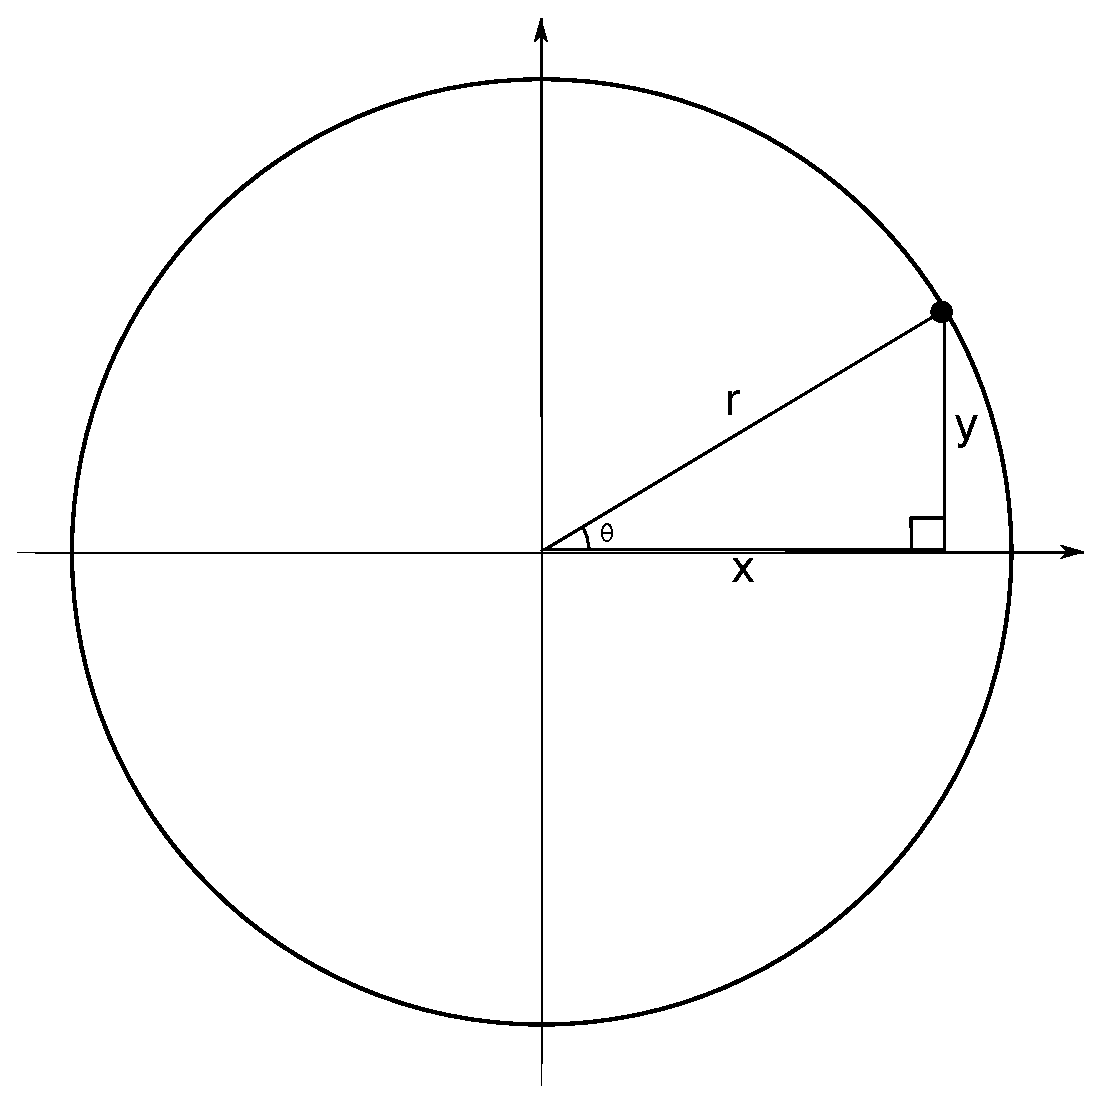
\includegraphics[width=8cm]{trig/img/circleTrig}

  \begin{subproblem}
  \item A function, sine, is defined to be
    \begin{eqnarray*}
      \sin(\theta) & = & \frac{y}{r}.
    \end{eqnarray*}
    Determine the formula for the value of $y$ given $r$ and $\theta$
    in terms of the sine function.
    \vfill
  \item A function, cosine, is defined to be
    \begin{eqnarray*}
      \cos(\theta) & = & \frac{x}{r}.
    \end{eqnarray*}
    Determine the formula for the value of $x$ given $r$ and $\theta$
    in terms of the cosine function.
    \vfill
  \end{subproblem}

\end{problem}


\actTitle{Basic Trigonomety}
\begin{problem}
\item Answer each of the following questions where the given point is $P(2,4)$.
  \begin{subproblem}
  \item Make a sketch of the coordinate plane and include the point
    $P(2,4)$. Draw the ray from the origin to the point. (Label your
    axes!)  \vfill
  \item Add a circle to your sketch show center is the origin and goes
    through the point. Label the angle $\theta$ as the angle between
    the ray and the $x$-axis.
  \item What is the radius of the circle?  
    \vspace{2em}
  \item Determine the values of the sine and cosine for the angle.
    \begin{eqnarray*}
      \sin(\theta) & = & \\ [10pt]
      \cos(\theta) & = & 
    \end{eqnarray*}
  \end{subproblem}

\clearpage

\item For each point below determine the radius and the value of the
  sine and cosine of the angle associated with each point.
  \begin{subproblem}
  \item $P(1,0)$
    \vfill
  \item $P(0,1)$
    \vfill
  \item $P(-1,0)$
    \vfill
  \item $P(0,-1)$
    \vfill
  \item $P\left(\frac{\sqrt{2}}{2},\frac{\sqrt{2}}{2}\right)$
    \vfill
  \end{subproblem}

\clearpage

\item The circle below is centered at the origin and has a radius of
  one.

  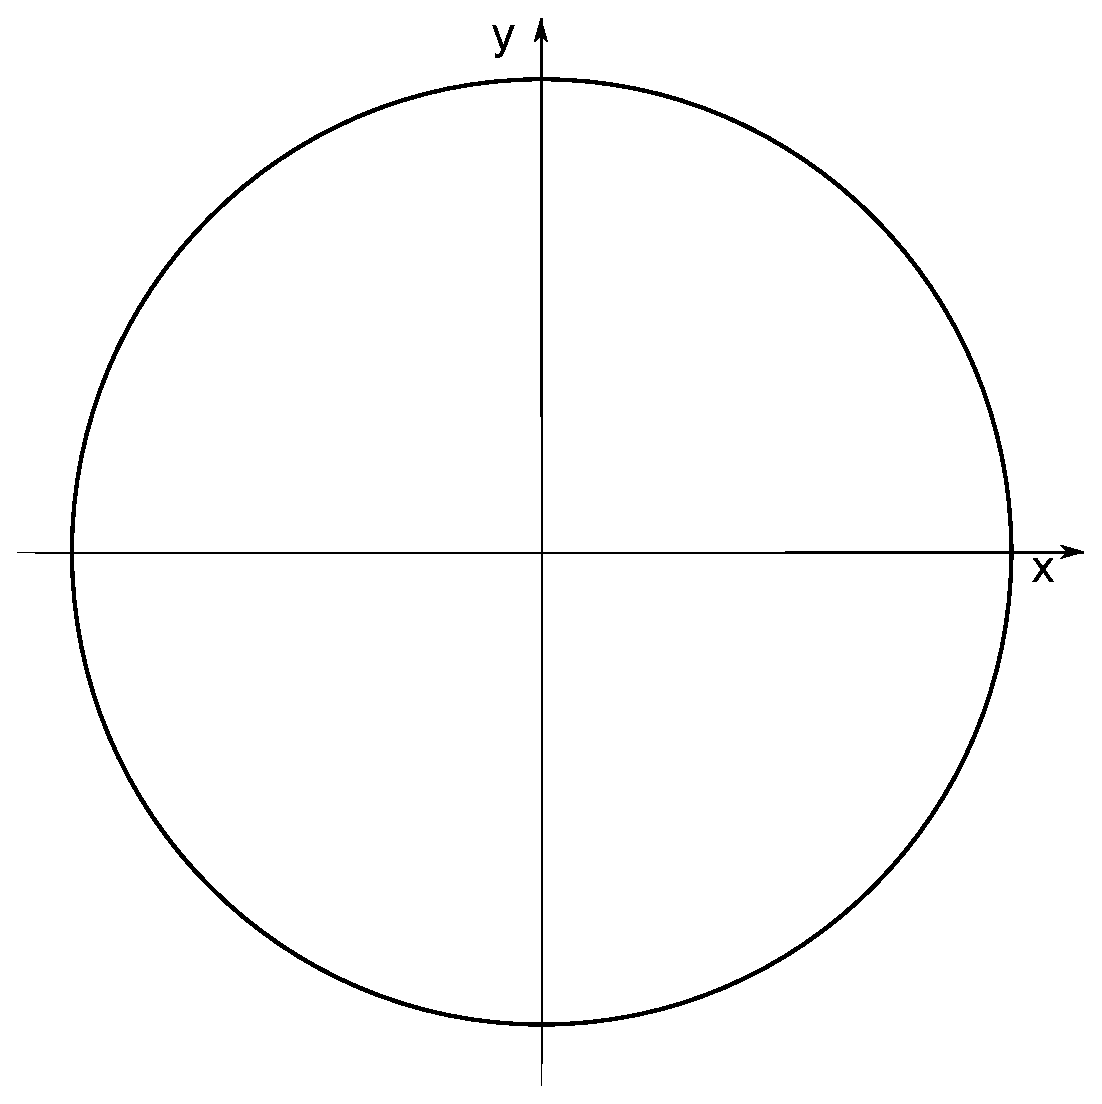
\includegraphics[width=16cm]{trig/img/blankCircle}

  \begin{subproblem}
  \item Mark the locations on the circle whose associated angles are
    0, $\pi/4$, $\pi/2$, $3\pi/4$, $\pi$, $5\pi/4$, $3\pi/2$, and
    $7\pi/4$.
    \clearpage

  \item Determine the $(x,y)$ coordinates for each angle.
    \vfill
  \item Determine the cosine and sine of each angle.
    \vfill
  \end{subproblem}

\end{problem}

\postClass

\begin{problem}
\item Briefly state two ideas from today's class.
  \begin{itemize}
  \item 
  \item 
  \end{itemize}
\item 
  \begin{subproblem}
    \item
  \end{subproblem}
\end{problem}


\propertiesTitle{The Unit Circle}

\begin{minipage}{0.5\linewidth}
  \begin{tikzpicture}[scale=3]
    \draw[step=0.5cm,gray!30,very thin] (-1.1,-1.1) grid (1.1,1.1);
    \draw (-1.1,0) -- (1.1,0); \draw (0,-1.1) -- (0,1.1); 
    \draw (0,0) circle [radius=1cm];

    \draw[black!80,thin] (.1cm,0cm) arc [start angle=0, end angle=30,radius=.1cm]; 
    \draw[red!80,thin] (30:1cm) -- ++(0,-0.5cm); 
    \draw[blue!80,thin] (0,0) -- (30:1cm); 
    \draw (10:0.35cm) node {$\pi/6$};
    \draw (0,1.2cm) node {$y$};
    \draw (1.2cm,0) node {$x$};

    \foreach \x in {-1,-0.5,0.5,1} 
       \draw (\x cm,1pt) -- (\x cm,-1pt) node[anchor=north,fill=white] {$\x$}; 
    \foreach \y in {-1,-0.5,0.5,1} 
       \draw (1pt,\y cm) -- (-1pt,\y cm) node[anchor=east,fill=white] {$\y$};
  \end{tikzpicture}
\end{minipage}
\begin{minipage}{0.5\linewidth}
\begin{tikzpicture}[scale=3]
\draw[step=0.5cm,gray!30,very thin] (-1.1,-1.1) grid (1.1,1.1);
\draw (-1.1,0) -- (1.1,0);
\draw (0,-1.1) -- (0,1.1);
\draw (0,0) circle [radius=1cm];

\draw[black!80,thin] (.1cm,0cm) arc [start angle=0, end angle=60,radius=.1cm];
\draw[red!80,thin] (0.5,0) -- (60:1cm);
\draw[blue!80,thin] (0,0) -- (60:1cm);
\draw (15:0.25cm) node {$\pi/3$};
\draw (0,1.2cm) node {$y$};
\draw (1.2cm,0) node {$x$};

\foreach \x in {-1,-0.5,0.5,1}
   \draw (\x cm,1pt) -- (\x cm,-1pt) node[anchor=north,fill=white] {$\x$};
\foreach \y in {-1,-0.5,0.5,1}
   \draw (1pt,\y cm) -- (-1pt,\y cm) node[anchor=east,fill=white] {$\y$};
\end{tikzpicture}
\end{minipage}

\begin{minipage}{0.5\linewidth}
  \begin{tikzpicture}[scale=3]
    \draw[step=0.5cm,gray!30,very thin] (-1.1,-1.1) grid (1.1,1.1);
    \draw (-1.1,0) -- (1.1,0); 
    \draw (0,-1.1) -- (0,1.1); \draw (0,0) circle [radius=1cm];

    \draw[black!80,thin] (.1cm,0cm) arc [start angle=0, end angle=150,radius=.1cm]; 
    \draw[red!80,thin] (150:1cm) -- ++(0,-0.5cm); 
    \draw[blue!80,thin] (0,0) -- (150:1cm); 
    \draw (25:0.25cm) node {$5\pi/6$};
    \draw (0,1.2cm) node {$y$};
    \draw (1.2cm,0) node {$x$};

    \foreach \x in {-1,-0.5,0.5,1} 
       \draw (\x cm,1pt) -- (\x cm,-1pt) node[anchor=north,fill=white] {$\x$}; 
    \foreach \y in {-1,-0.5,0.5,1} 
    \draw (1pt,\y cm) -- (-1pt,\y cm) node[anchor=east,fill=white] {$\y$};
  \end{tikzpicture}
\end{minipage}
\begin{minipage}{0.5\linewidth}
\begin{tikzpicture}[scale=3]
\draw[step=0.5cm,gray!30,very thin] (-1.1,-1.1) grid (1.1,1.1);
\draw (-1.1,0) -- (1.1,0);
\draw (0,-1.1) -- (0,1.1);
\draw (0,0) circle [radius=1cm];

\draw[black!80,thin] (.1cm,0cm) arc [start angle=0, end angle=120,radius=.1cm];
\draw[red!80,thin] (-0.5,0) -- (120:1cm);
\draw[blue!80,thin] (0,0) -- (120:1cm);
\draw (15:0.25cm) node {$2\pi/3$};
\draw (0,1.2cm) node {$y$};
\draw (1.2cm,0) node {$x$};

\foreach \x in {-1,-0.5,0.5,1}
   \draw (\x cm,1pt) -- (\x cm,-1pt) node[anchor=north,fill=white] {$\x$};
\foreach \y in {-1,-0.5,0.5,1}{
   \draw (-1pt,\y cm) -- (1pt,\y cm);
   \draw (12pt,\y cm) node[anchor=east,fill=white] {$\y$};
 }
\end{tikzpicture}
\end{minipage}

\clearpage

\begin{minipage}{0.5\linewidth}
  \begin{tikzpicture}[scale=3]
    \draw[step=0.5cm,gray!30,very thin] (-1.1,-1.1) grid (1.1,1.1);
    \draw (-1.1,0) -- (1.1,0); 
    \draw (0,-1.1) -- (0,1.1); \draw (0,0) circle [radius=1cm];

    \draw[black!80,thin] (.1cm,0cm) arc [start angle=0, end angle=210,radius=.1cm]; 
    \draw[red!80,thin] (210:1cm) -- ++(0,0.5cm); 
    \draw[blue!80,thin] (0,0) -- (210:1cm); 
    \draw (25:0.25cm) node {$7\pi/6$};
    \draw (0,1.2cm) node {$y$};
    \draw (1.2cm,0) node {$x$};

    \foreach \x in {-1,-0.5,0.5,1} 
       \draw (\x cm,1pt) -- (\x cm,-1pt) node[anchor=north,fill=white] {$\x$}; 
    \foreach \y in {-1,-0.5,0.5,1} 
    \draw (1pt,\y cm) -- (-1pt,\y cm) node[anchor=east,fill=white] {$\y$};
  \end{tikzpicture}
\end{minipage}
\begin{minipage}{0.5\linewidth}
\begin{tikzpicture}[scale=3]
\draw[step=0.5cm,gray!30,very thin] (-1.1,-1.1) grid (1.1,1.1);
\draw (-1.1,0) -- (1.1,0);
\draw (0,-1.1) -- (0,1.1);
\draw (0,0) circle [radius=1cm];

\draw[black!80,thin] (.1cm,0cm) arc [start angle=0, end angle=240,radius=.1cm];
\draw[red!80,thin] (-0.5,0) -- (240:1cm);
\draw[blue!80,thin] (0,0) -- (240:1cm);
\draw (15:0.25cm) node {$4\pi/3$};
\draw (0,1.2cm) node {$y$};
\draw (1.2cm,0) node {$x$};

\foreach \x in {-1,-0.5,0.5,1}
   \draw (\x cm,1pt) -- (\x cm,-1pt) node[anchor=north,fill=white] {$\x$};
\foreach \y in {-1,-0.5,0.5,1}{
   \draw (-1pt,\y cm) -- (1pt,\y cm);
   \draw (12pt,\y cm) node[anchor=east,fill=white] {$\y$};
 }
\end{tikzpicture}
\end{minipage}


\begin{minipage}{0.5\linewidth}
  \begin{tikzpicture}[scale=3]
    \draw[step=0.5cm,gray!30,very thin] (-1.1,-1.1) grid (1.1,1.1);
    \draw (-1.1,0) -- (1.1,0); 
    \draw (0,-1.1) -- (0,1.1); \draw (0,0) circle [radius=1cm];

    \draw[black!80,thin] (.1cm,0cm) arc [start angle=0, end angle=330,radius=.1cm]; 
    \draw[red!80,thin] (330:1cm) -- ++(0,0.5cm); 
    \draw[blue!80,thin] (0,0) -- (330:1cm); 
    \draw (25:0.25cm) node {$11\pi/6$};
    \draw (0,1.2cm) node {$y$};
    \draw (1.2cm,0) node {$x$};

    \foreach \x in {-1,-0.5,0.5,1} 
       \draw (\x cm,1pt) -- (\x cm,-1pt) node[anchor=north,fill=white] {$\x$}; 
    \foreach \y in {-1,-0.5,0.5,1} 
    \draw (1pt,\y cm) -- (-1pt,\y cm) node[anchor=east,fill=white] {$\y$};
  \end{tikzpicture}
\end{minipage}
\begin{minipage}{0.5\linewidth}
\begin{tikzpicture}[scale=3]
  \draw[step=0.5cm,gray!30,very thin] (-1.1,-1.1) grid (1.1,1.1);
  \draw (-1.1,0) -- (1.1,0);
  \draw (0,-1.1) -- (0,1.1);
  \draw (0,0) circle [radius=1cm];

  \draw[black!80,thin] (.1cm,0cm) arc [start angle=0, end angle=300,radius=.1cm];
  \draw[red!80,thin] (0.5,0) -- (300:1cm);
  \draw[blue!80,thin] (0,0) -- (300:1cm);
  \draw (15:0.25cm) node {$4\pi/3$};
  \draw (0,1.2cm) node {$y$};
  \draw (1.2cm,0) node {$x$};

  \foreach \x in {-1,-0.5,0.5,1}
    \draw (\x cm,1pt) -- (\x cm,-1pt) node[anchor=north,fill=white] {$\x$};
  \foreach \y in {-1,-0.5,0.5,1}{
      \draw (-1pt,\y cm) -- (1pt,\y cm);
      \draw (12pt,\y cm) node[anchor=east,fill=white] {$\y$};
  }
\end{tikzpicture}
\end{minipage}


%%% Local Variables:
%%% mode: latex
%%% TeX-master: "../labManual"
%%% End:



%=========================================================================
% Start of 
%=========================================================================
\preClass{Trigonometric Functions}

\begin{problem}
\item An ant starts at the coordinate $P(1,0)$, and it moves
  counter-clockwise around a circle of radius one centered at the
  origin. It moves at a constant 1 meter per minute.
  \begin{subproblem}
  \item Sketch a plot of the ant's path.
    \vfill
  \item Sketch a plot of the ant's $x$-coordinate as a function of
    time. 
    \vfill
  \item Sketch a plot of the ant's $y$-coordinate as a function of
    time.
    \vfill
  \end{subproblem}
\end{problem}


\actTitle{Trigonometric Functions}
\begin{problem}
\item 
  \begin{subproblem}
    \item Make a sketch of the sine function.

      \hspace*{-6em}
      \scalebox{0.7}{%% Creator: Matplotlib, PGF backend
%%
%% To include the figure in your LaTeX document, write
%%   \input{<filename>.pgf}
%%
%% Make sure the required packages are loaded in your preamble
%%   \usepackage{pgf}
%%
%% Figures using additional raster images can only be included by \input if
%% they are in the same directory as the main LaTeX file. For loading figures
%% from other directories you can use the `import` package
%%   \usepackage{import}
%% and then include the figures with
%%   \import{<path to file>}{<filename>.pgf}
%%
%% Matplotlib used the following preamble
%%   \usepackage{fontspec}
%%   \setmainfont{Bitstream Vera Serif}
%%   \setsansfont{Bitstream Vera Sans}
%%   \setmonofont{Bitstream Vera Sans Mono}
%%
\begingroup%
\makeatletter%
\begin{pgfpicture}%
\pgfpathrectangle{\pgfpointorigin}{\pgfqpoint{8.000000in}{6.000000in}}%
\pgfusepath{use as bounding box, clip}%
\begin{pgfscope}%
\pgfsetbuttcap%
\pgfsetmiterjoin%
\definecolor{currentfill}{rgb}{1.000000,1.000000,1.000000}%
\pgfsetfillcolor{currentfill}%
\pgfsetlinewidth{0.000000pt}%
\definecolor{currentstroke}{rgb}{1.000000,1.000000,1.000000}%
\pgfsetstrokecolor{currentstroke}%
\pgfsetdash{}{0pt}%
\pgfpathmoveto{\pgfqpoint{0.000000in}{0.000000in}}%
\pgfpathlineto{\pgfqpoint{8.000000in}{0.000000in}}%
\pgfpathlineto{\pgfqpoint{8.000000in}{6.000000in}}%
\pgfpathlineto{\pgfqpoint{0.000000in}{6.000000in}}%
\pgfpathclose%
\pgfusepath{fill}%
\end{pgfscope}%
\begin{pgfscope}%
\pgfsetbuttcap%
\pgfsetmiterjoin%
\definecolor{currentfill}{rgb}{1.000000,1.000000,1.000000}%
\pgfsetfillcolor{currentfill}%
\pgfsetlinewidth{0.000000pt}%
\definecolor{currentstroke}{rgb}{0.000000,0.000000,0.000000}%
\pgfsetstrokecolor{currentstroke}%
\pgfsetstrokeopacity{0.000000}%
\pgfsetdash{}{0pt}%
\pgfpathmoveto{\pgfqpoint{1.000000in}{0.600000in}}%
\pgfpathlineto{\pgfqpoint{7.200000in}{0.600000in}}%
\pgfpathlineto{\pgfqpoint{7.200000in}{5.400000in}}%
\pgfpathlineto{\pgfqpoint{1.000000in}{5.400000in}}%
\pgfpathclose%
\pgfusepath{fill}%
\end{pgfscope}%
\begin{pgfscope}%
\pgfsetrectcap%
\pgfsetmiterjoin%
\pgfsetlinewidth{0.000000pt}%
\definecolor{currentstroke}{rgb}{0.000000,0.000000,0.000000}%
\pgfsetstrokecolor{currentstroke}%
\pgfsetstrokeopacity{0.000000}%
\pgfsetdash{}{0pt}%
\pgfpathmoveto{\pgfqpoint{1.000000in}{5.400000in}}%
\pgfpathlineto{\pgfqpoint{7.200000in}{5.400000in}}%
\pgfusepath{}%
\end{pgfscope}%
\begin{pgfscope}%
\pgfsetrectcap%
\pgfsetmiterjoin%
\pgfsetlinewidth{0.000000pt}%
\definecolor{currentstroke}{rgb}{0.000000,0.000000,0.000000}%
\pgfsetstrokecolor{currentstroke}%
\pgfsetstrokeopacity{0.000000}%
\pgfsetdash{}{0pt}%
\pgfpathmoveto{\pgfqpoint{7.200000in}{0.600000in}}%
\pgfpathlineto{\pgfqpoint{7.200000in}{5.400000in}}%
\pgfusepath{}%
\end{pgfscope}%
\begin{pgfscope}%
\pgfsetrectcap%
\pgfsetmiterjoin%
\pgfsetlinewidth{1.003750pt}%
\definecolor{currentstroke}{rgb}{0.000000,0.000000,0.000000}%
\pgfsetstrokecolor{currentstroke}%
\pgfsetdash{}{0pt}%
\pgfpathmoveto{\pgfqpoint{1.000000in}{3.000000in}}%
\pgfpathlineto{\pgfqpoint{7.200000in}{3.000000in}}%
\pgfusepath{stroke}%
\end{pgfscope}%
\begin{pgfscope}%
\pgfsetrectcap%
\pgfsetmiterjoin%
\pgfsetlinewidth{1.003750pt}%
\definecolor{currentstroke}{rgb}{0.000000,0.000000,0.000000}%
\pgfsetstrokecolor{currentstroke}%
\pgfsetdash{}{0pt}%
\pgfpathmoveto{\pgfqpoint{1.000000in}{0.600000in}}%
\pgfpathlineto{\pgfqpoint{1.000000in}{5.400000in}}%
\pgfusepath{stroke}%
\end{pgfscope}%
\begin{pgfscope}%
\pgfsetbuttcap%
\pgfsetroundjoin%
\pgfsetlinewidth{0.501875pt}%
\definecolor{currentstroke}{rgb}{0.000000,0.000000,0.000000}%
\pgfsetstrokecolor{currentstroke}%
\pgfsetdash{{1.000000pt}{3.000000pt}}{0.000000pt}%
\pgfpathmoveto{\pgfqpoint{1.000000in}{0.600000in}}%
\pgfpathlineto{\pgfqpoint{1.000000in}{5.400000in}}%
\pgfusepath{stroke}%
\end{pgfscope}%
\begin{pgfscope}%
\pgfsetbuttcap%
\pgfsetroundjoin%
\definecolor{currentfill}{rgb}{0.000000,0.000000,0.000000}%
\pgfsetfillcolor{currentfill}%
\pgfsetlinewidth{0.501875pt}%
\definecolor{currentstroke}{rgb}{0.000000,0.000000,0.000000}%
\pgfsetstrokecolor{currentstroke}%
\pgfsetdash{}{0pt}%
\pgfsys@defobject{currentmarker}{\pgfqpoint{0.000000in}{0.000000in}}{\pgfqpoint{0.000000in}{0.055556in}}{%
\pgfpathmoveto{\pgfqpoint{0.000000in}{0.000000in}}%
\pgfpathlineto{\pgfqpoint{0.000000in}{0.055556in}}%
\pgfusepath{stroke,fill}%
}%
\begin{pgfscope}%
\pgfsys@transformshift{1.000000in}{3.000000in}%
\pgfsys@useobject{currentmarker}{}%
\end{pgfscope}%
\end{pgfscope}%
\begin{pgfscope}%
\pgftext[x=1.000000in,y=2.944444in,,top]{\sffamily\fontsize{12.000000}{14.400000}\selectfont 0}%
\end{pgfscope}%
\begin{pgfscope}%
\pgfsetbuttcap%
\pgfsetroundjoin%
\pgfsetlinewidth{0.501875pt}%
\definecolor{currentstroke}{rgb}{0.000000,0.000000,0.000000}%
\pgfsetstrokecolor{currentstroke}%
\pgfsetdash{{1.000000pt}{3.000000pt}}{0.000000pt}%
\pgfpathmoveto{\pgfqpoint{2.202338in}{0.600000in}}%
\pgfpathlineto{\pgfqpoint{2.202338in}{5.400000in}}%
\pgfusepath{stroke}%
\end{pgfscope}%
\begin{pgfscope}%
\pgfsetbuttcap%
\pgfsetroundjoin%
\definecolor{currentfill}{rgb}{0.000000,0.000000,0.000000}%
\pgfsetfillcolor{currentfill}%
\pgfsetlinewidth{0.501875pt}%
\definecolor{currentstroke}{rgb}{0.000000,0.000000,0.000000}%
\pgfsetstrokecolor{currentstroke}%
\pgfsetdash{}{0pt}%
\pgfsys@defobject{currentmarker}{\pgfqpoint{0.000000in}{0.000000in}}{\pgfqpoint{0.000000in}{0.055556in}}{%
\pgfpathmoveto{\pgfqpoint{0.000000in}{0.000000in}}%
\pgfpathlineto{\pgfqpoint{0.000000in}{0.055556in}}%
\pgfusepath{stroke,fill}%
}%
\begin{pgfscope}%
\pgfsys@transformshift{2.202338in}{3.000000in}%
\pgfsys@useobject{currentmarker}{}%
\end{pgfscope}%
\end{pgfscope}%
\begin{pgfscope}%
\pgftext[x=2.202338in,y=2.944444in,,top]{\sffamily\fontsize{12.000000}{14.400000}\selectfont \(\displaystyle \frac{\pi}{2}\)}%
\end{pgfscope}%
\begin{pgfscope}%
\pgfsetbuttcap%
\pgfsetroundjoin%
\pgfsetlinewidth{0.501875pt}%
\definecolor{currentstroke}{rgb}{0.000000,0.000000,0.000000}%
\pgfsetstrokecolor{currentstroke}%
\pgfsetdash{{1.000000pt}{3.000000pt}}{0.000000pt}%
\pgfpathmoveto{\pgfqpoint{3.404676in}{0.600000in}}%
\pgfpathlineto{\pgfqpoint{3.404676in}{5.400000in}}%
\pgfusepath{stroke}%
\end{pgfscope}%
\begin{pgfscope}%
\pgfsetbuttcap%
\pgfsetroundjoin%
\definecolor{currentfill}{rgb}{0.000000,0.000000,0.000000}%
\pgfsetfillcolor{currentfill}%
\pgfsetlinewidth{0.501875pt}%
\definecolor{currentstroke}{rgb}{0.000000,0.000000,0.000000}%
\pgfsetstrokecolor{currentstroke}%
\pgfsetdash{}{0pt}%
\pgfsys@defobject{currentmarker}{\pgfqpoint{0.000000in}{0.000000in}}{\pgfqpoint{0.000000in}{0.055556in}}{%
\pgfpathmoveto{\pgfqpoint{0.000000in}{0.000000in}}%
\pgfpathlineto{\pgfqpoint{0.000000in}{0.055556in}}%
\pgfusepath{stroke,fill}%
}%
\begin{pgfscope}%
\pgfsys@transformshift{3.404676in}{3.000000in}%
\pgfsys@useobject{currentmarker}{}%
\end{pgfscope}%
\end{pgfscope}%
\begin{pgfscope}%
\pgftext[x=3.404676in,y=2.944444in,,top]{\sffamily\fontsize{12.000000}{14.400000}\selectfont \(\displaystyle \pi\)}%
\end{pgfscope}%
\begin{pgfscope}%
\pgfsetbuttcap%
\pgfsetroundjoin%
\pgfsetlinewidth{0.501875pt}%
\definecolor{currentstroke}{rgb}{0.000000,0.000000,0.000000}%
\pgfsetstrokecolor{currentstroke}%
\pgfsetdash{{1.000000pt}{3.000000pt}}{0.000000pt}%
\pgfpathmoveto{\pgfqpoint{4.607014in}{0.600000in}}%
\pgfpathlineto{\pgfqpoint{4.607014in}{5.400000in}}%
\pgfusepath{stroke}%
\end{pgfscope}%
\begin{pgfscope}%
\pgfsetbuttcap%
\pgfsetroundjoin%
\definecolor{currentfill}{rgb}{0.000000,0.000000,0.000000}%
\pgfsetfillcolor{currentfill}%
\pgfsetlinewidth{0.501875pt}%
\definecolor{currentstroke}{rgb}{0.000000,0.000000,0.000000}%
\pgfsetstrokecolor{currentstroke}%
\pgfsetdash{}{0pt}%
\pgfsys@defobject{currentmarker}{\pgfqpoint{0.000000in}{0.000000in}}{\pgfqpoint{0.000000in}{0.055556in}}{%
\pgfpathmoveto{\pgfqpoint{0.000000in}{0.000000in}}%
\pgfpathlineto{\pgfqpoint{0.000000in}{0.055556in}}%
\pgfusepath{stroke,fill}%
}%
\begin{pgfscope}%
\pgfsys@transformshift{4.607014in}{3.000000in}%
\pgfsys@useobject{currentmarker}{}%
\end{pgfscope}%
\end{pgfscope}%
\begin{pgfscope}%
\pgftext[x=4.607014in,y=2.944444in,,top]{\sffamily\fontsize{12.000000}{14.400000}\selectfont \(\displaystyle \frac{3\pi}{2}\)}%
\end{pgfscope}%
\begin{pgfscope}%
\pgfsetbuttcap%
\pgfsetroundjoin%
\pgfsetlinewidth{0.501875pt}%
\definecolor{currentstroke}{rgb}{0.000000,0.000000,0.000000}%
\pgfsetstrokecolor{currentstroke}%
\pgfsetdash{{1.000000pt}{3.000000pt}}{0.000000pt}%
\pgfpathmoveto{\pgfqpoint{5.809352in}{0.600000in}}%
\pgfpathlineto{\pgfqpoint{5.809352in}{5.400000in}}%
\pgfusepath{stroke}%
\end{pgfscope}%
\begin{pgfscope}%
\pgfsetbuttcap%
\pgfsetroundjoin%
\definecolor{currentfill}{rgb}{0.000000,0.000000,0.000000}%
\pgfsetfillcolor{currentfill}%
\pgfsetlinewidth{0.501875pt}%
\definecolor{currentstroke}{rgb}{0.000000,0.000000,0.000000}%
\pgfsetstrokecolor{currentstroke}%
\pgfsetdash{}{0pt}%
\pgfsys@defobject{currentmarker}{\pgfqpoint{0.000000in}{0.000000in}}{\pgfqpoint{0.000000in}{0.055556in}}{%
\pgfpathmoveto{\pgfqpoint{0.000000in}{0.000000in}}%
\pgfpathlineto{\pgfqpoint{0.000000in}{0.055556in}}%
\pgfusepath{stroke,fill}%
}%
\begin{pgfscope}%
\pgfsys@transformshift{5.809352in}{3.000000in}%
\pgfsys@useobject{currentmarker}{}%
\end{pgfscope}%
\end{pgfscope}%
\begin{pgfscope}%
\pgftext[x=5.809352in,y=2.944444in,,top]{\sffamily\fontsize{12.000000}{14.400000}\selectfont \(\displaystyle 2\pi\)}%
\end{pgfscope}%
\begin{pgfscope}%
\pgfsetbuttcap%
\pgfsetroundjoin%
\pgfsetlinewidth{0.501875pt}%
\definecolor{currentstroke}{rgb}{0.000000,0.000000,0.000000}%
\pgfsetstrokecolor{currentstroke}%
\pgfsetdash{{1.000000pt}{3.000000pt}}{0.000000pt}%
\pgfpathmoveto{\pgfqpoint{7.011690in}{0.600000in}}%
\pgfpathlineto{\pgfqpoint{7.011690in}{5.400000in}}%
\pgfusepath{stroke}%
\end{pgfscope}%
\begin{pgfscope}%
\pgfsetbuttcap%
\pgfsetroundjoin%
\definecolor{currentfill}{rgb}{0.000000,0.000000,0.000000}%
\pgfsetfillcolor{currentfill}%
\pgfsetlinewidth{0.501875pt}%
\definecolor{currentstroke}{rgb}{0.000000,0.000000,0.000000}%
\pgfsetstrokecolor{currentstroke}%
\pgfsetdash{}{0pt}%
\pgfsys@defobject{currentmarker}{\pgfqpoint{0.000000in}{0.000000in}}{\pgfqpoint{0.000000in}{0.055556in}}{%
\pgfpathmoveto{\pgfqpoint{0.000000in}{0.000000in}}%
\pgfpathlineto{\pgfqpoint{0.000000in}{0.055556in}}%
\pgfusepath{stroke,fill}%
}%
\begin{pgfscope}%
\pgfsys@transformshift{7.011690in}{3.000000in}%
\pgfsys@useobject{currentmarker}{}%
\end{pgfscope}%
\end{pgfscope}%
\begin{pgfscope}%
\pgftext[x=7.011690in,y=2.944444in,,top]{\sffamily\fontsize{12.000000}{14.400000}\selectfont \(\displaystyle \frac{5\pi}{2}\)}%
\end{pgfscope}%
\begin{pgfscope}%
\pgftext[x=6.890000in,y=2.760000in,,top]{\sffamily\fontsize{12.000000}{14.400000}\selectfont \(\displaystyle \theta\)}%
\end{pgfscope}%
\begin{pgfscope}%
\pgfsetbuttcap%
\pgfsetroundjoin%
\pgfsetlinewidth{0.501875pt}%
\definecolor{currentstroke}{rgb}{0.000000,0.000000,0.000000}%
\pgfsetstrokecolor{currentstroke}%
\pgfsetdash{{1.000000pt}{3.000000pt}}{0.000000pt}%
\pgfpathmoveto{\pgfqpoint{1.000000in}{0.818182in}}%
\pgfpathlineto{\pgfqpoint{7.200000in}{0.818182in}}%
\pgfusepath{stroke}%
\end{pgfscope}%
\begin{pgfscope}%
\pgfsetbuttcap%
\pgfsetroundjoin%
\definecolor{currentfill}{rgb}{0.000000,0.000000,0.000000}%
\pgfsetfillcolor{currentfill}%
\pgfsetlinewidth{0.501875pt}%
\definecolor{currentstroke}{rgb}{0.000000,0.000000,0.000000}%
\pgfsetstrokecolor{currentstroke}%
\pgfsetdash{}{0pt}%
\pgfsys@defobject{currentmarker}{\pgfqpoint{0.000000in}{0.000000in}}{\pgfqpoint{0.055556in}{0.000000in}}{%
\pgfpathmoveto{\pgfqpoint{0.000000in}{0.000000in}}%
\pgfpathlineto{\pgfqpoint{0.055556in}{0.000000in}}%
\pgfusepath{stroke,fill}%
}%
\begin{pgfscope}%
\pgfsys@transformshift{1.000000in}{0.818182in}%
\pgfsys@useobject{currentmarker}{}%
\end{pgfscope}%
\end{pgfscope}%
\begin{pgfscope}%
\pgftext[x=0.944444in,y=0.818182in,right,]{\sffamily\fontsize{12.000000}{14.400000}\selectfont \(\displaystyle -1\)}%
\end{pgfscope}%
\begin{pgfscope}%
\pgfsetbuttcap%
\pgfsetroundjoin%
\pgfsetlinewidth{0.501875pt}%
\definecolor{currentstroke}{rgb}{0.000000,0.000000,0.000000}%
\pgfsetstrokecolor{currentstroke}%
\pgfsetdash{{1.000000pt}{3.000000pt}}{0.000000pt}%
\pgfpathmoveto{\pgfqpoint{1.000000in}{3.000000in}}%
\pgfpathlineto{\pgfqpoint{7.200000in}{3.000000in}}%
\pgfusepath{stroke}%
\end{pgfscope}%
\begin{pgfscope}%
\pgfsetbuttcap%
\pgfsetroundjoin%
\definecolor{currentfill}{rgb}{0.000000,0.000000,0.000000}%
\pgfsetfillcolor{currentfill}%
\pgfsetlinewidth{0.501875pt}%
\definecolor{currentstroke}{rgb}{0.000000,0.000000,0.000000}%
\pgfsetstrokecolor{currentstroke}%
\pgfsetdash{}{0pt}%
\pgfsys@defobject{currentmarker}{\pgfqpoint{0.000000in}{0.000000in}}{\pgfqpoint{0.055556in}{0.000000in}}{%
\pgfpathmoveto{\pgfqpoint{0.000000in}{0.000000in}}%
\pgfpathlineto{\pgfqpoint{0.055556in}{0.000000in}}%
\pgfusepath{stroke,fill}%
}%
\begin{pgfscope}%
\pgfsys@transformshift{1.000000in}{3.000000in}%
\pgfsys@useobject{currentmarker}{}%
\end{pgfscope}%
\end{pgfscope}%
\begin{pgfscope}%
\pgftext[x=0.944444in,y=3.000000in,right,]{\sffamily\fontsize{12.000000}{14.400000}\selectfont \(\displaystyle 0\)}%
\end{pgfscope}%
\begin{pgfscope}%
\pgfsetbuttcap%
\pgfsetroundjoin%
\pgfsetlinewidth{0.501875pt}%
\definecolor{currentstroke}{rgb}{0.000000,0.000000,0.000000}%
\pgfsetstrokecolor{currentstroke}%
\pgfsetdash{{1.000000pt}{3.000000pt}}{0.000000pt}%
\pgfpathmoveto{\pgfqpoint{1.000000in}{5.181818in}}%
\pgfpathlineto{\pgfqpoint{7.200000in}{5.181818in}}%
\pgfusepath{stroke}%
\end{pgfscope}%
\begin{pgfscope}%
\pgfsetbuttcap%
\pgfsetroundjoin%
\definecolor{currentfill}{rgb}{0.000000,0.000000,0.000000}%
\pgfsetfillcolor{currentfill}%
\pgfsetlinewidth{0.501875pt}%
\definecolor{currentstroke}{rgb}{0.000000,0.000000,0.000000}%
\pgfsetstrokecolor{currentstroke}%
\pgfsetdash{}{0pt}%
\pgfsys@defobject{currentmarker}{\pgfqpoint{0.000000in}{0.000000in}}{\pgfqpoint{0.055556in}{0.000000in}}{%
\pgfpathmoveto{\pgfqpoint{0.000000in}{0.000000in}}%
\pgfpathlineto{\pgfqpoint{0.055556in}{0.000000in}}%
\pgfusepath{stroke,fill}%
}%
\begin{pgfscope}%
\pgfsys@transformshift{1.000000in}{5.181818in}%
\pgfsys@useobject{currentmarker}{}%
\end{pgfscope}%
\end{pgfscope}%
\begin{pgfscope}%
\pgftext[x=0.944444in,y=5.181818in,right,]{\sffamily\fontsize{12.000000}{14.400000}\selectfont \(\displaystyle 1\)}%
\end{pgfscope}%
\begin{pgfscope}%
\pgftext[x=0.690000in,y=5.160000in,,bottom,rotate=90.000000]{\sffamily\fontsize{12.000000}{14.400000}\selectfont sin}%
\end{pgfscope}%
\begin{pgfscope}%
\pgftext[x=4.100000in,y=5.469444in,,base]{\sffamily\fontsize{14.400000}{17.280000}\selectfont Sine}%
\end{pgfscope}%
\end{pgfpicture}%
\makeatother%
\endgroup%
}

    \item Over what values of $\theta$ does the sine function repeat
      itself?
      \vfill

    \item For what value of $a$ is 
      \begin{eqnarray*}
        \sin(\theta) & = & \sin(\theta-a)?
      \end{eqnarray*}

    \item Is the sine function an invertible function?

      \clearpage
    \item Make a sketch of the cosine function.

      \hspace*{-6em}
      \scalebox{0.7}{%% Creator: Matplotlib, PGF backend
%%
%% To include the figure in your LaTeX document, write
%%   \input{<filename>.pgf}
%%
%% Make sure the required packages are loaded in your preamble
%%   \usepackage{pgf}
%%
%% Figures using additional raster images can only be included by \input if
%% they are in the same directory as the main LaTeX file. For loading figures
%% from other directories you can use the `import` package
%%   \usepackage{import}
%% and then include the figures with
%%   \import{<path to file>}{<filename>.pgf}
%%
%% Matplotlib used the following preamble
%%   \usepackage{fontspec}
%%   \setmainfont{Bitstream Vera Serif}
%%   \setsansfont{Bitstream Vera Sans}
%%   \setmonofont{Bitstream Vera Sans Mono}
%%
\begingroup%
\makeatletter%
\begin{pgfpicture}%
\pgfpathrectangle{\pgfpointorigin}{\pgfqpoint{10.000000in}{3.500000in}}%
\pgfusepath{use as bounding box, clip}%
\begin{pgfscope}%
\pgfsetbuttcap%
\pgfsetmiterjoin%
\definecolor{currentfill}{rgb}{1.000000,1.000000,1.000000}%
\pgfsetfillcolor{currentfill}%
\pgfsetlinewidth{0.000000pt}%
\definecolor{currentstroke}{rgb}{1.000000,1.000000,1.000000}%
\pgfsetstrokecolor{currentstroke}%
\pgfsetdash{}{0pt}%
\pgfpathmoveto{\pgfqpoint{0.000000in}{0.000000in}}%
\pgfpathlineto{\pgfqpoint{10.000000in}{0.000000in}}%
\pgfpathlineto{\pgfqpoint{10.000000in}{3.500000in}}%
\pgfpathlineto{\pgfqpoint{0.000000in}{3.500000in}}%
\pgfpathclose%
\pgfusepath{fill}%
\end{pgfscope}%
\begin{pgfscope}%
\pgfsetbuttcap%
\pgfsetmiterjoin%
\definecolor{currentfill}{rgb}{1.000000,1.000000,1.000000}%
\pgfsetfillcolor{currentfill}%
\pgfsetlinewidth{0.000000pt}%
\definecolor{currentstroke}{rgb}{0.000000,0.000000,0.000000}%
\pgfsetstrokecolor{currentstroke}%
\pgfsetstrokeopacity{0.000000}%
\pgfsetdash{}{0pt}%
\pgfpathmoveto{\pgfqpoint{1.250000in}{0.350000in}}%
\pgfpathlineto{\pgfqpoint{9.000000in}{0.350000in}}%
\pgfpathlineto{\pgfqpoint{9.000000in}{3.150000in}}%
\pgfpathlineto{\pgfqpoint{1.250000in}{3.150000in}}%
\pgfpathclose%
\pgfusepath{fill}%
\end{pgfscope}%
\begin{pgfscope}%
\pgfsetrectcap%
\pgfsetmiterjoin%
\pgfsetlinewidth{0.000000pt}%
\definecolor{currentstroke}{rgb}{0.000000,0.000000,0.000000}%
\pgfsetstrokecolor{currentstroke}%
\pgfsetstrokeopacity{0.000000}%
\pgfsetdash{}{0pt}%
\pgfpathmoveto{\pgfqpoint{1.250000in}{3.150000in}}%
\pgfpathlineto{\pgfqpoint{9.000000in}{3.150000in}}%
\pgfusepath{}%
\end{pgfscope}%
\begin{pgfscope}%
\pgfsetrectcap%
\pgfsetmiterjoin%
\pgfsetlinewidth{0.000000pt}%
\definecolor{currentstroke}{rgb}{0.000000,0.000000,0.000000}%
\pgfsetstrokecolor{currentstroke}%
\pgfsetstrokeopacity{0.000000}%
\pgfsetdash{}{0pt}%
\pgfpathmoveto{\pgfqpoint{9.000000in}{0.350000in}}%
\pgfpathlineto{\pgfqpoint{9.000000in}{3.150000in}}%
\pgfusepath{}%
\end{pgfscope}%
\begin{pgfscope}%
\pgfsetrectcap%
\pgfsetmiterjoin%
\pgfsetlinewidth{1.003750pt}%
\definecolor{currentstroke}{rgb}{0.000000,0.000000,0.000000}%
\pgfsetstrokecolor{currentstroke}%
\pgfsetdash{}{0pt}%
\pgfpathmoveto{\pgfqpoint{1.250000in}{1.750000in}}%
\pgfpathlineto{\pgfqpoint{9.000000in}{1.750000in}}%
\pgfusepath{stroke}%
\end{pgfscope}%
\begin{pgfscope}%
\pgfsetrectcap%
\pgfsetmiterjoin%
\pgfsetlinewidth{1.003750pt}%
\definecolor{currentstroke}{rgb}{0.000000,0.000000,0.000000}%
\pgfsetstrokecolor{currentstroke}%
\pgfsetdash{}{0pt}%
\pgfpathmoveto{\pgfqpoint{1.250000in}{0.350000in}}%
\pgfpathlineto{\pgfqpoint{1.250000in}{3.150000in}}%
\pgfusepath{stroke}%
\end{pgfscope}%
\begin{pgfscope}%
\pgfsetbuttcap%
\pgfsetroundjoin%
\pgfsetlinewidth{0.501875pt}%
\definecolor{currentstroke}{rgb}{0.000000,0.000000,0.000000}%
\pgfsetstrokecolor{currentstroke}%
\pgfsetdash{{1.000000pt}{3.000000pt}}{0.000000pt}%
\pgfpathmoveto{\pgfqpoint{1.250000in}{0.350000in}}%
\pgfpathlineto{\pgfqpoint{1.250000in}{3.150000in}}%
\pgfusepath{stroke}%
\end{pgfscope}%
\begin{pgfscope}%
\pgfsetbuttcap%
\pgfsetroundjoin%
\definecolor{currentfill}{rgb}{0.000000,0.000000,0.000000}%
\pgfsetfillcolor{currentfill}%
\pgfsetlinewidth{0.501875pt}%
\definecolor{currentstroke}{rgb}{0.000000,0.000000,0.000000}%
\pgfsetstrokecolor{currentstroke}%
\pgfsetdash{}{0pt}%
\pgfsys@defobject{currentmarker}{\pgfqpoint{0.000000in}{0.000000in}}{\pgfqpoint{0.000000in}{0.055556in}}{%
\pgfpathmoveto{\pgfqpoint{0.000000in}{0.000000in}}%
\pgfpathlineto{\pgfqpoint{0.000000in}{0.055556in}}%
\pgfusepath{stroke,fill}%
}%
\begin{pgfscope}%
\pgfsys@transformshift{1.250000in}{1.750000in}%
\pgfsys@useobject{currentmarker}{}%
\end{pgfscope}%
\end{pgfscope}%
\begin{pgfscope}%
\pgftext[x=1.250000in,y=1.694444in,,top]{\sffamily\fontsize{12.000000}{14.400000}\selectfont 0}%
\end{pgfscope}%
\begin{pgfscope}%
\pgfsetbuttcap%
\pgfsetroundjoin%
\pgfsetlinewidth{0.501875pt}%
\definecolor{currentstroke}{rgb}{0.000000,0.000000,0.000000}%
\pgfsetstrokecolor{currentstroke}%
\pgfsetdash{{1.000000pt}{3.000000pt}}{0.000000pt}%
\pgfpathmoveto{\pgfqpoint{1.887365in}{0.350000in}}%
\pgfpathlineto{\pgfqpoint{1.887365in}{3.150000in}}%
\pgfusepath{stroke}%
\end{pgfscope}%
\begin{pgfscope}%
\pgfsetbuttcap%
\pgfsetroundjoin%
\definecolor{currentfill}{rgb}{0.000000,0.000000,0.000000}%
\pgfsetfillcolor{currentfill}%
\pgfsetlinewidth{0.501875pt}%
\definecolor{currentstroke}{rgb}{0.000000,0.000000,0.000000}%
\pgfsetstrokecolor{currentstroke}%
\pgfsetdash{}{0pt}%
\pgfsys@defobject{currentmarker}{\pgfqpoint{0.000000in}{0.000000in}}{\pgfqpoint{0.000000in}{0.055556in}}{%
\pgfpathmoveto{\pgfqpoint{0.000000in}{0.000000in}}%
\pgfpathlineto{\pgfqpoint{0.000000in}{0.055556in}}%
\pgfusepath{stroke,fill}%
}%
\begin{pgfscope}%
\pgfsys@transformshift{1.887365in}{1.750000in}%
\pgfsys@useobject{currentmarker}{}%
\end{pgfscope}%
\end{pgfscope}%
\begin{pgfscope}%
\pgftext[x=1.887365in,y=1.694444in,,top]{\sffamily\fontsize{12.000000}{14.400000}\selectfont \(\displaystyle \frac{\pi}{2}\)}%
\end{pgfscope}%
\begin{pgfscope}%
\pgfsetbuttcap%
\pgfsetroundjoin%
\pgfsetlinewidth{0.501875pt}%
\definecolor{currentstroke}{rgb}{0.000000,0.000000,0.000000}%
\pgfsetstrokecolor{currentstroke}%
\pgfsetdash{{1.000000pt}{3.000000pt}}{0.000000pt}%
\pgfpathmoveto{\pgfqpoint{2.524730in}{0.350000in}}%
\pgfpathlineto{\pgfqpoint{2.524730in}{3.150000in}}%
\pgfusepath{stroke}%
\end{pgfscope}%
\begin{pgfscope}%
\pgfsetbuttcap%
\pgfsetroundjoin%
\definecolor{currentfill}{rgb}{0.000000,0.000000,0.000000}%
\pgfsetfillcolor{currentfill}%
\pgfsetlinewidth{0.501875pt}%
\definecolor{currentstroke}{rgb}{0.000000,0.000000,0.000000}%
\pgfsetstrokecolor{currentstroke}%
\pgfsetdash{}{0pt}%
\pgfsys@defobject{currentmarker}{\pgfqpoint{0.000000in}{0.000000in}}{\pgfqpoint{0.000000in}{0.055556in}}{%
\pgfpathmoveto{\pgfqpoint{0.000000in}{0.000000in}}%
\pgfpathlineto{\pgfqpoint{0.000000in}{0.055556in}}%
\pgfusepath{stroke,fill}%
}%
\begin{pgfscope}%
\pgfsys@transformshift{2.524730in}{1.750000in}%
\pgfsys@useobject{currentmarker}{}%
\end{pgfscope}%
\end{pgfscope}%
\begin{pgfscope}%
\pgftext[x=2.524730in,y=1.694444in,,top]{\sffamily\fontsize{12.000000}{14.400000}\selectfont \(\displaystyle \pi\)}%
\end{pgfscope}%
\begin{pgfscope}%
\pgfsetbuttcap%
\pgfsetroundjoin%
\pgfsetlinewidth{0.501875pt}%
\definecolor{currentstroke}{rgb}{0.000000,0.000000,0.000000}%
\pgfsetstrokecolor{currentstroke}%
\pgfsetdash{{1.000000pt}{3.000000pt}}{0.000000pt}%
\pgfpathmoveto{\pgfqpoint{3.162095in}{0.350000in}}%
\pgfpathlineto{\pgfqpoint{3.162095in}{3.150000in}}%
\pgfusepath{stroke}%
\end{pgfscope}%
\begin{pgfscope}%
\pgfsetbuttcap%
\pgfsetroundjoin%
\definecolor{currentfill}{rgb}{0.000000,0.000000,0.000000}%
\pgfsetfillcolor{currentfill}%
\pgfsetlinewidth{0.501875pt}%
\definecolor{currentstroke}{rgb}{0.000000,0.000000,0.000000}%
\pgfsetstrokecolor{currentstroke}%
\pgfsetdash{}{0pt}%
\pgfsys@defobject{currentmarker}{\pgfqpoint{0.000000in}{0.000000in}}{\pgfqpoint{0.000000in}{0.055556in}}{%
\pgfpathmoveto{\pgfqpoint{0.000000in}{0.000000in}}%
\pgfpathlineto{\pgfqpoint{0.000000in}{0.055556in}}%
\pgfusepath{stroke,fill}%
}%
\begin{pgfscope}%
\pgfsys@transformshift{3.162095in}{1.750000in}%
\pgfsys@useobject{currentmarker}{}%
\end{pgfscope}%
\end{pgfscope}%
\begin{pgfscope}%
\pgftext[x=3.162095in,y=1.694444in,,top]{\sffamily\fontsize{12.000000}{14.400000}\selectfont \(\displaystyle \frac{3\pi}{2}\)}%
\end{pgfscope}%
\begin{pgfscope}%
\pgfsetbuttcap%
\pgfsetroundjoin%
\pgfsetlinewidth{0.501875pt}%
\definecolor{currentstroke}{rgb}{0.000000,0.000000,0.000000}%
\pgfsetstrokecolor{currentstroke}%
\pgfsetdash{{1.000000pt}{3.000000pt}}{0.000000pt}%
\pgfpathmoveto{\pgfqpoint{3.799460in}{0.350000in}}%
\pgfpathlineto{\pgfqpoint{3.799460in}{3.150000in}}%
\pgfusepath{stroke}%
\end{pgfscope}%
\begin{pgfscope}%
\pgfsetbuttcap%
\pgfsetroundjoin%
\definecolor{currentfill}{rgb}{0.000000,0.000000,0.000000}%
\pgfsetfillcolor{currentfill}%
\pgfsetlinewidth{0.501875pt}%
\definecolor{currentstroke}{rgb}{0.000000,0.000000,0.000000}%
\pgfsetstrokecolor{currentstroke}%
\pgfsetdash{}{0pt}%
\pgfsys@defobject{currentmarker}{\pgfqpoint{0.000000in}{0.000000in}}{\pgfqpoint{0.000000in}{0.055556in}}{%
\pgfpathmoveto{\pgfqpoint{0.000000in}{0.000000in}}%
\pgfpathlineto{\pgfqpoint{0.000000in}{0.055556in}}%
\pgfusepath{stroke,fill}%
}%
\begin{pgfscope}%
\pgfsys@transformshift{3.799460in}{1.750000in}%
\pgfsys@useobject{currentmarker}{}%
\end{pgfscope}%
\end{pgfscope}%
\begin{pgfscope}%
\pgftext[x=3.799460in,y=1.694444in,,top]{\sffamily\fontsize{12.000000}{14.400000}\selectfont \(\displaystyle 2\pi\)}%
\end{pgfscope}%
\begin{pgfscope}%
\pgfsetbuttcap%
\pgfsetroundjoin%
\pgfsetlinewidth{0.501875pt}%
\definecolor{currentstroke}{rgb}{0.000000,0.000000,0.000000}%
\pgfsetstrokecolor{currentstroke}%
\pgfsetdash{{1.000000pt}{3.000000pt}}{0.000000pt}%
\pgfpathmoveto{\pgfqpoint{4.436825in}{0.350000in}}%
\pgfpathlineto{\pgfqpoint{4.436825in}{3.150000in}}%
\pgfusepath{stroke}%
\end{pgfscope}%
\begin{pgfscope}%
\pgfsetbuttcap%
\pgfsetroundjoin%
\definecolor{currentfill}{rgb}{0.000000,0.000000,0.000000}%
\pgfsetfillcolor{currentfill}%
\pgfsetlinewidth{0.501875pt}%
\definecolor{currentstroke}{rgb}{0.000000,0.000000,0.000000}%
\pgfsetstrokecolor{currentstroke}%
\pgfsetdash{}{0pt}%
\pgfsys@defobject{currentmarker}{\pgfqpoint{0.000000in}{0.000000in}}{\pgfqpoint{0.000000in}{0.055556in}}{%
\pgfpathmoveto{\pgfqpoint{0.000000in}{0.000000in}}%
\pgfpathlineto{\pgfqpoint{0.000000in}{0.055556in}}%
\pgfusepath{stroke,fill}%
}%
\begin{pgfscope}%
\pgfsys@transformshift{4.436825in}{1.750000in}%
\pgfsys@useobject{currentmarker}{}%
\end{pgfscope}%
\end{pgfscope}%
\begin{pgfscope}%
\pgftext[x=4.436825in,y=1.694444in,,top]{\sffamily\fontsize{12.000000}{14.400000}\selectfont \(\displaystyle \frac{5\pi}{2}\)}%
\end{pgfscope}%
\begin{pgfscope}%
\pgfsetbuttcap%
\pgfsetroundjoin%
\pgfsetlinewidth{0.501875pt}%
\definecolor{currentstroke}{rgb}{0.000000,0.000000,0.000000}%
\pgfsetstrokecolor{currentstroke}%
\pgfsetdash{{1.000000pt}{3.000000pt}}{0.000000pt}%
\pgfpathmoveto{\pgfqpoint{5.074190in}{0.350000in}}%
\pgfpathlineto{\pgfqpoint{5.074190in}{3.150000in}}%
\pgfusepath{stroke}%
\end{pgfscope}%
\begin{pgfscope}%
\pgfsetbuttcap%
\pgfsetroundjoin%
\definecolor{currentfill}{rgb}{0.000000,0.000000,0.000000}%
\pgfsetfillcolor{currentfill}%
\pgfsetlinewidth{0.501875pt}%
\definecolor{currentstroke}{rgb}{0.000000,0.000000,0.000000}%
\pgfsetstrokecolor{currentstroke}%
\pgfsetdash{}{0pt}%
\pgfsys@defobject{currentmarker}{\pgfqpoint{0.000000in}{0.000000in}}{\pgfqpoint{0.000000in}{0.055556in}}{%
\pgfpathmoveto{\pgfqpoint{0.000000in}{0.000000in}}%
\pgfpathlineto{\pgfqpoint{0.000000in}{0.055556in}}%
\pgfusepath{stroke,fill}%
}%
\begin{pgfscope}%
\pgfsys@transformshift{5.074190in}{1.750000in}%
\pgfsys@useobject{currentmarker}{}%
\end{pgfscope}%
\end{pgfscope}%
\begin{pgfscope}%
\pgftext[x=5.074190in,y=1.694444in,,top]{\sffamily\fontsize{12.000000}{14.400000}\selectfont \(\displaystyle 3\pi\)}%
\end{pgfscope}%
\begin{pgfscope}%
\pgfsetbuttcap%
\pgfsetroundjoin%
\pgfsetlinewidth{0.501875pt}%
\definecolor{currentstroke}{rgb}{0.000000,0.000000,0.000000}%
\pgfsetstrokecolor{currentstroke}%
\pgfsetdash{{1.000000pt}{3.000000pt}}{0.000000pt}%
\pgfpathmoveto{\pgfqpoint{5.711555in}{0.350000in}}%
\pgfpathlineto{\pgfqpoint{5.711555in}{3.150000in}}%
\pgfusepath{stroke}%
\end{pgfscope}%
\begin{pgfscope}%
\pgfsetbuttcap%
\pgfsetroundjoin%
\definecolor{currentfill}{rgb}{0.000000,0.000000,0.000000}%
\pgfsetfillcolor{currentfill}%
\pgfsetlinewidth{0.501875pt}%
\definecolor{currentstroke}{rgb}{0.000000,0.000000,0.000000}%
\pgfsetstrokecolor{currentstroke}%
\pgfsetdash{}{0pt}%
\pgfsys@defobject{currentmarker}{\pgfqpoint{0.000000in}{0.000000in}}{\pgfqpoint{0.000000in}{0.055556in}}{%
\pgfpathmoveto{\pgfqpoint{0.000000in}{0.000000in}}%
\pgfpathlineto{\pgfqpoint{0.000000in}{0.055556in}}%
\pgfusepath{stroke,fill}%
}%
\begin{pgfscope}%
\pgfsys@transformshift{5.711555in}{1.750000in}%
\pgfsys@useobject{currentmarker}{}%
\end{pgfscope}%
\end{pgfscope}%
\begin{pgfscope}%
\pgftext[x=5.711555in,y=1.694444in,,top]{\sffamily\fontsize{12.000000}{14.400000}\selectfont \(\displaystyle \frac{7\pi}{2}\)}%
\end{pgfscope}%
\begin{pgfscope}%
\pgfsetbuttcap%
\pgfsetroundjoin%
\pgfsetlinewidth{0.501875pt}%
\definecolor{currentstroke}{rgb}{0.000000,0.000000,0.000000}%
\pgfsetstrokecolor{currentstroke}%
\pgfsetdash{{1.000000pt}{3.000000pt}}{0.000000pt}%
\pgfpathmoveto{\pgfqpoint{6.348920in}{0.350000in}}%
\pgfpathlineto{\pgfqpoint{6.348920in}{3.150000in}}%
\pgfusepath{stroke}%
\end{pgfscope}%
\begin{pgfscope}%
\pgfsetbuttcap%
\pgfsetroundjoin%
\definecolor{currentfill}{rgb}{0.000000,0.000000,0.000000}%
\pgfsetfillcolor{currentfill}%
\pgfsetlinewidth{0.501875pt}%
\definecolor{currentstroke}{rgb}{0.000000,0.000000,0.000000}%
\pgfsetstrokecolor{currentstroke}%
\pgfsetdash{}{0pt}%
\pgfsys@defobject{currentmarker}{\pgfqpoint{0.000000in}{0.000000in}}{\pgfqpoint{0.000000in}{0.055556in}}{%
\pgfpathmoveto{\pgfqpoint{0.000000in}{0.000000in}}%
\pgfpathlineto{\pgfqpoint{0.000000in}{0.055556in}}%
\pgfusepath{stroke,fill}%
}%
\begin{pgfscope}%
\pgfsys@transformshift{6.348920in}{1.750000in}%
\pgfsys@useobject{currentmarker}{}%
\end{pgfscope}%
\end{pgfscope}%
\begin{pgfscope}%
\pgftext[x=6.348920in,y=1.694444in,,top]{\sffamily\fontsize{12.000000}{14.400000}\selectfont \(\displaystyle 4\pi\)}%
\end{pgfscope}%
\begin{pgfscope}%
\pgfsetbuttcap%
\pgfsetroundjoin%
\pgfsetlinewidth{0.501875pt}%
\definecolor{currentstroke}{rgb}{0.000000,0.000000,0.000000}%
\pgfsetstrokecolor{currentstroke}%
\pgfsetdash{{1.000000pt}{3.000000pt}}{0.000000pt}%
\pgfpathmoveto{\pgfqpoint{6.986285in}{0.350000in}}%
\pgfpathlineto{\pgfqpoint{6.986285in}{3.150000in}}%
\pgfusepath{stroke}%
\end{pgfscope}%
\begin{pgfscope}%
\pgfsetbuttcap%
\pgfsetroundjoin%
\definecolor{currentfill}{rgb}{0.000000,0.000000,0.000000}%
\pgfsetfillcolor{currentfill}%
\pgfsetlinewidth{0.501875pt}%
\definecolor{currentstroke}{rgb}{0.000000,0.000000,0.000000}%
\pgfsetstrokecolor{currentstroke}%
\pgfsetdash{}{0pt}%
\pgfsys@defobject{currentmarker}{\pgfqpoint{0.000000in}{0.000000in}}{\pgfqpoint{0.000000in}{0.055556in}}{%
\pgfpathmoveto{\pgfqpoint{0.000000in}{0.000000in}}%
\pgfpathlineto{\pgfqpoint{0.000000in}{0.055556in}}%
\pgfusepath{stroke,fill}%
}%
\begin{pgfscope}%
\pgfsys@transformshift{6.986285in}{1.750000in}%
\pgfsys@useobject{currentmarker}{}%
\end{pgfscope}%
\end{pgfscope}%
\begin{pgfscope}%
\pgftext[x=6.986285in,y=1.694444in,,top]{\sffamily\fontsize{12.000000}{14.400000}\selectfont \(\displaystyle \frac{9\pi}{2}\)}%
\end{pgfscope}%
\begin{pgfscope}%
\pgfsetbuttcap%
\pgfsetroundjoin%
\pgfsetlinewidth{0.501875pt}%
\definecolor{currentstroke}{rgb}{0.000000,0.000000,0.000000}%
\pgfsetstrokecolor{currentstroke}%
\pgfsetdash{{1.000000pt}{3.000000pt}}{0.000000pt}%
\pgfpathmoveto{\pgfqpoint{7.623650in}{0.350000in}}%
\pgfpathlineto{\pgfqpoint{7.623650in}{3.150000in}}%
\pgfusepath{stroke}%
\end{pgfscope}%
\begin{pgfscope}%
\pgfsetbuttcap%
\pgfsetroundjoin%
\definecolor{currentfill}{rgb}{0.000000,0.000000,0.000000}%
\pgfsetfillcolor{currentfill}%
\pgfsetlinewidth{0.501875pt}%
\definecolor{currentstroke}{rgb}{0.000000,0.000000,0.000000}%
\pgfsetstrokecolor{currentstroke}%
\pgfsetdash{}{0pt}%
\pgfsys@defobject{currentmarker}{\pgfqpoint{0.000000in}{0.000000in}}{\pgfqpoint{0.000000in}{0.055556in}}{%
\pgfpathmoveto{\pgfqpoint{0.000000in}{0.000000in}}%
\pgfpathlineto{\pgfqpoint{0.000000in}{0.055556in}}%
\pgfusepath{stroke,fill}%
}%
\begin{pgfscope}%
\pgfsys@transformshift{7.623650in}{1.750000in}%
\pgfsys@useobject{currentmarker}{}%
\end{pgfscope}%
\end{pgfscope}%
\begin{pgfscope}%
\pgftext[x=7.623650in,y=1.694444in,,top]{\sffamily\fontsize{12.000000}{14.400000}\selectfont \(\displaystyle 5\pi\)}%
\end{pgfscope}%
\begin{pgfscope}%
\pgfsetbuttcap%
\pgfsetroundjoin%
\pgfsetlinewidth{0.501875pt}%
\definecolor{currentstroke}{rgb}{0.000000,0.000000,0.000000}%
\pgfsetstrokecolor{currentstroke}%
\pgfsetdash{{1.000000pt}{3.000000pt}}{0.000000pt}%
\pgfpathmoveto{\pgfqpoint{8.261015in}{0.350000in}}%
\pgfpathlineto{\pgfqpoint{8.261015in}{3.150000in}}%
\pgfusepath{stroke}%
\end{pgfscope}%
\begin{pgfscope}%
\pgfsetbuttcap%
\pgfsetroundjoin%
\definecolor{currentfill}{rgb}{0.000000,0.000000,0.000000}%
\pgfsetfillcolor{currentfill}%
\pgfsetlinewidth{0.501875pt}%
\definecolor{currentstroke}{rgb}{0.000000,0.000000,0.000000}%
\pgfsetstrokecolor{currentstroke}%
\pgfsetdash{}{0pt}%
\pgfsys@defobject{currentmarker}{\pgfqpoint{0.000000in}{0.000000in}}{\pgfqpoint{0.000000in}{0.055556in}}{%
\pgfpathmoveto{\pgfqpoint{0.000000in}{0.000000in}}%
\pgfpathlineto{\pgfqpoint{0.000000in}{0.055556in}}%
\pgfusepath{stroke,fill}%
}%
\begin{pgfscope}%
\pgfsys@transformshift{8.261015in}{1.750000in}%
\pgfsys@useobject{currentmarker}{}%
\end{pgfscope}%
\end{pgfscope}%
\begin{pgfscope}%
\pgftext[x=8.261015in,y=1.694444in,,top]{\sffamily\fontsize{12.000000}{14.400000}\selectfont \(\displaystyle \frac{11\pi}{2}\)}%
\end{pgfscope}%
\begin{pgfscope}%
\pgfsetbuttcap%
\pgfsetroundjoin%
\pgfsetlinewidth{0.501875pt}%
\definecolor{currentstroke}{rgb}{0.000000,0.000000,0.000000}%
\pgfsetstrokecolor{currentstroke}%
\pgfsetdash{{1.000000pt}{3.000000pt}}{0.000000pt}%
\pgfpathmoveto{\pgfqpoint{8.898380in}{0.350000in}}%
\pgfpathlineto{\pgfqpoint{8.898380in}{3.150000in}}%
\pgfusepath{stroke}%
\end{pgfscope}%
\begin{pgfscope}%
\pgfsetbuttcap%
\pgfsetroundjoin%
\definecolor{currentfill}{rgb}{0.000000,0.000000,0.000000}%
\pgfsetfillcolor{currentfill}%
\pgfsetlinewidth{0.501875pt}%
\definecolor{currentstroke}{rgb}{0.000000,0.000000,0.000000}%
\pgfsetstrokecolor{currentstroke}%
\pgfsetdash{}{0pt}%
\pgfsys@defobject{currentmarker}{\pgfqpoint{0.000000in}{0.000000in}}{\pgfqpoint{0.000000in}{0.055556in}}{%
\pgfpathmoveto{\pgfqpoint{0.000000in}{0.000000in}}%
\pgfpathlineto{\pgfqpoint{0.000000in}{0.055556in}}%
\pgfusepath{stroke,fill}%
}%
\begin{pgfscope}%
\pgfsys@transformshift{8.898380in}{1.750000in}%
\pgfsys@useobject{currentmarker}{}%
\end{pgfscope}%
\end{pgfscope}%
\begin{pgfscope}%
\pgftext[x=8.898380in,y=1.694444in,,top]{\sffamily\fontsize{12.000000}{14.400000}\selectfont \(\displaystyle 6\pi\)}%
\end{pgfscope}%
\begin{pgfscope}%
\pgftext[x=8.612500in,y=1.890000in,,top]{\sffamily\fontsize{12.000000}{14.400000}\selectfont \(\displaystyle \theta\)}%
\end{pgfscope}%
\begin{pgfscope}%
\pgfsetbuttcap%
\pgfsetroundjoin%
\pgfsetlinewidth{0.501875pt}%
\definecolor{currentstroke}{rgb}{0.000000,0.000000,0.000000}%
\pgfsetstrokecolor{currentstroke}%
\pgfsetdash{{1.000000pt}{3.000000pt}}{0.000000pt}%
\pgfpathmoveto{\pgfqpoint{1.250000in}{0.477273in}}%
\pgfpathlineto{\pgfqpoint{9.000000in}{0.477273in}}%
\pgfusepath{stroke}%
\end{pgfscope}%
\begin{pgfscope}%
\pgfsetbuttcap%
\pgfsetroundjoin%
\definecolor{currentfill}{rgb}{0.000000,0.000000,0.000000}%
\pgfsetfillcolor{currentfill}%
\pgfsetlinewidth{0.501875pt}%
\definecolor{currentstroke}{rgb}{0.000000,0.000000,0.000000}%
\pgfsetstrokecolor{currentstroke}%
\pgfsetdash{}{0pt}%
\pgfsys@defobject{currentmarker}{\pgfqpoint{0.000000in}{0.000000in}}{\pgfqpoint{0.055556in}{0.000000in}}{%
\pgfpathmoveto{\pgfqpoint{0.000000in}{0.000000in}}%
\pgfpathlineto{\pgfqpoint{0.055556in}{0.000000in}}%
\pgfusepath{stroke,fill}%
}%
\begin{pgfscope}%
\pgfsys@transformshift{1.250000in}{0.477273in}%
\pgfsys@useobject{currentmarker}{}%
\end{pgfscope}%
\end{pgfscope}%
\begin{pgfscope}%
\pgftext[x=1.194444in,y=0.477273in,right,]{\sffamily\fontsize{12.000000}{14.400000}\selectfont \(\displaystyle -1\)}%
\end{pgfscope}%
\begin{pgfscope}%
\pgfsetbuttcap%
\pgfsetroundjoin%
\pgfsetlinewidth{0.501875pt}%
\definecolor{currentstroke}{rgb}{0.000000,0.000000,0.000000}%
\pgfsetstrokecolor{currentstroke}%
\pgfsetdash{{1.000000pt}{3.000000pt}}{0.000000pt}%
\pgfpathmoveto{\pgfqpoint{1.250000in}{1.750000in}}%
\pgfpathlineto{\pgfqpoint{9.000000in}{1.750000in}}%
\pgfusepath{stroke}%
\end{pgfscope}%
\begin{pgfscope}%
\pgfsetbuttcap%
\pgfsetroundjoin%
\definecolor{currentfill}{rgb}{0.000000,0.000000,0.000000}%
\pgfsetfillcolor{currentfill}%
\pgfsetlinewidth{0.501875pt}%
\definecolor{currentstroke}{rgb}{0.000000,0.000000,0.000000}%
\pgfsetstrokecolor{currentstroke}%
\pgfsetdash{}{0pt}%
\pgfsys@defobject{currentmarker}{\pgfqpoint{0.000000in}{0.000000in}}{\pgfqpoint{0.055556in}{0.000000in}}{%
\pgfpathmoveto{\pgfqpoint{0.000000in}{0.000000in}}%
\pgfpathlineto{\pgfqpoint{0.055556in}{0.000000in}}%
\pgfusepath{stroke,fill}%
}%
\begin{pgfscope}%
\pgfsys@transformshift{1.250000in}{1.750000in}%
\pgfsys@useobject{currentmarker}{}%
\end{pgfscope}%
\end{pgfscope}%
\begin{pgfscope}%
\pgftext[x=1.194444in,y=1.750000in,right,]{\sffamily\fontsize{12.000000}{14.400000}\selectfont \(\displaystyle 0\)}%
\end{pgfscope}%
\begin{pgfscope}%
\pgfsetbuttcap%
\pgfsetroundjoin%
\pgfsetlinewidth{0.501875pt}%
\definecolor{currentstroke}{rgb}{0.000000,0.000000,0.000000}%
\pgfsetstrokecolor{currentstroke}%
\pgfsetdash{{1.000000pt}{3.000000pt}}{0.000000pt}%
\pgfpathmoveto{\pgfqpoint{1.250000in}{3.022727in}}%
\pgfpathlineto{\pgfqpoint{9.000000in}{3.022727in}}%
\pgfusepath{stroke}%
\end{pgfscope}%
\begin{pgfscope}%
\pgfsetbuttcap%
\pgfsetroundjoin%
\definecolor{currentfill}{rgb}{0.000000,0.000000,0.000000}%
\pgfsetfillcolor{currentfill}%
\pgfsetlinewidth{0.501875pt}%
\definecolor{currentstroke}{rgb}{0.000000,0.000000,0.000000}%
\pgfsetstrokecolor{currentstroke}%
\pgfsetdash{}{0pt}%
\pgfsys@defobject{currentmarker}{\pgfqpoint{0.000000in}{0.000000in}}{\pgfqpoint{0.055556in}{0.000000in}}{%
\pgfpathmoveto{\pgfqpoint{0.000000in}{0.000000in}}%
\pgfpathlineto{\pgfqpoint{0.055556in}{0.000000in}}%
\pgfusepath{stroke,fill}%
}%
\begin{pgfscope}%
\pgfsys@transformshift{1.250000in}{3.022727in}%
\pgfsys@useobject{currentmarker}{}%
\end{pgfscope}%
\end{pgfscope}%
\begin{pgfscope}%
\pgftext[x=1.194444in,y=3.022727in,right,]{\sffamily\fontsize{12.000000}{14.400000}\selectfont \(\displaystyle 1\)}%
\end{pgfscope}%
\begin{pgfscope}%
\pgftext[x=1.017500in,y=3.010000in,,bottom,rotate=90.000000]{\sffamily\fontsize{12.000000}{14.400000}\selectfont cos}%
\end{pgfscope}%
\begin{pgfscope}%
\pgftext[x=5.125000in,y=3.219444in,,base]{\sffamily\fontsize{14.400000}{17.280000}\selectfont Cosine}%
\end{pgfscope}%
\end{pgfpicture}%
\makeatother%
\endgroup%
}

    \item Over what values of $\theta$ does the cosine function repeat
      itself?
      \vfill

    \item For what value of $a$ is 
      \begin{eqnarray*}
        \cos(\theta) & = & \cos(\theta-a)?
      \end{eqnarray*}

    \item Is the cosine function an invertible function?

  \end{subproblem}

  \clearpage

\item What is the relationship between the sine and cosine functions?
  For each relationship below determine the value and use the unit
  circle to explain why these relationships should be expected.
  \begin{subproblem}
  \item Determine a value of $a$ where
    \begin{eqnarray*}
      \cos(\theta) & = & \sin(\theta+a).
    \end{eqnarray*}
    \vfill
  \item Determine a value of $a$ where
    \begin{eqnarray*}
      \cos(\theta) & = & -\sin(\theta+a).
    \end{eqnarray*}
    \vfill

    \clearpage

  \item Determine values of $a$, and $b$ so that the function
    \begin{eqnarray*}
      f(\theta) & = & a\sin(\theta)+b
    \end{eqnarray*}
    oscillates between 2 and 6.
    \vfill

  \item Determine values of $a$, and $b$ so that the function
    \begin{eqnarray*}
      f(\theta) & = & a\sin(\theta)+b
    \end{eqnarray*}
    oscillates between -5 and -3.
    \vfill


  \item Determine values of $a$, and $b$ so that the function
    \begin{eqnarray*}
      f(\theta) & = & a\sin(\theta)+b
    \end{eqnarray*}
    oscillates between -1 and 4.
    \vfill
  \end{subproblem}

\end{problem}

\postClass

\begin{problem}
\item Briefly state two ideas from today's class.
  \begin{itemize}
  \item 
  \item 
  \end{itemize}
\item 
  \begin{subproblem}
    \item
  \end{subproblem}
\end{problem}


%%% Local Variables:
%%% mode: latex
%%% TeX-master: "../labManual"
%%% End:



%=========================================================================
% Start of
%=========================================================================
\preClass{Graphs of Trigonometric Functions}

\begin{problem}
\item Make a sketch of the sine function.

  \hspace*{-3em}
  \begin{tikzpicture}[y=2cm, x=1.2cm,font=\sffamily]
      % bounds
      \def\lowX{0.0}
      \pgfmathtruncatemacro\startX{round(0.5+\lowX)}
      \pgfmathsetmacro\nextXValue{int(\startX+1)}
      \def\highX{12}
      \def\lowY{-1.25}
      \def\highY{1.25}
      \pgfmathsetmacro\nextYValue{int(\lowY+1)}
      % ticks
      \draw[step = 1, gray, very thin,dashed,opacity=0.85] (0, \lowY) grid ( \highX,\highY);
      % axis
      \draw[thick,->] (0,0) -- coordinate (x axis mid) (\highX,0) node[anchor = south west] {$\theta$};
      \draw[thick,->] (0,\lowY) -- coordinate (y axis mid) (0,\highY) node[anchor = north east] {Sine};

      \draw (1pt, 1) -- (-1pt, 1) node[yshift=-6,xshift=-1,anchor=east] { 1};
      \draw (1pt,-1) -- (-1pt,-1) node[yshift=-6,xshift=-1,anchor=east] {-1};

      \draw (1,1pt) -- (1,-1pt) node[yshift=-1,xshift=0,anchor=north east] {$\frac{ \pi}{2}$};
      \foreach \x in {3,5,...,\highX} {
        \draw (\x,1pt) -- (\x,-1pt) node[yshift=-8,xshift=1,anchor=east] {$\frac{\x\pi}{2}$};
      }
      \draw (2,1pt) -- (2,-1pt) node[yshift=-1,xshift=-1,anchor=north east] {$\pi$};
      \foreach \x in {2,3,...,6} {
        \draw (2*\x,1pt) -- (2*\x,-1pt) node[yshift=-7,xshift=3,anchor=east] {$\x\pi$};
      }
      \draw (6,1.3) node [anchor=south] {The Sine Function};
    \end{tikzpicture}

\item Make a sketch of the sine function shifted left $\frac{\pi}{2}$ units.

  \hspace*{-3em}
  \begin{tikzpicture}[y=2cm, x=1.2cm,font=\sffamily]
      % bounds
      \def\lowX{0.0}
      \pgfmathtruncatemacro\startX{round(0.5+\lowX)}
      \pgfmathsetmacro\nextXValue{int(\startX+1)}
      \def\highX{12}
      \def\lowY{-1.25}
      \def\highY{1.25}
      \pgfmathsetmacro\nextYValue{int(\lowY+1)}
      % ticks
      \draw[step = 1, gray, very thin,dashed,opacity=0.85] (0, \lowY) grid ( \highX,\highY);
      % axis
      \draw[thick,->] (0,0) -- coordinate (x axis mid) (\highX,0) node[anchor = south west] {$\theta$};
      \draw[thick,->] (0,\lowY) -- coordinate (y axis mid) (0,\highY) node[anchor = north east] {Sine};

      \draw (1pt, 1) -- (-1pt, 1) node[yshift=-6,xshift=-1,anchor=east] { 1};
      \draw (1pt,-1) -- (-1pt,-1) node[yshift=-6,xshift=-1,anchor=east] {-1};

      \draw (1,1pt) -- (1,-1pt) node[yshift=-1,xshift=0,anchor=north east] {$\frac{ \pi}{2}$};
      \foreach \x in {3,5,...,\highX} {
        \draw (\x,1pt) -- (\x,-1pt) node[yshift=-8,xshift=1,anchor=east] {$\frac{\x\pi}{2}$};
      }
      \draw (2,1pt) -- (2,-1pt) node[yshift=-1,xshift=-1,anchor=north east] {$\pi$};
      \foreach \x in {2,3,...,6} {
        \draw (2*\x,1pt) -- (2*\x,-1pt) node[yshift=-7,xshift=3,anchor=east] {$\x\pi$};
      }
      \draw (6,1.3) node [anchor=south] {The Sine Function};
    \end{tikzpicture}

  \clearpage

\item Make a sketch of the cosine function.

  \hspace*{-5em}
  \begin{tikzpicture}[y=2cm, x=1.2cm,font=\sffamily]
      % bounds
      \def\lowX{0.0}
      \pgfmathtruncatemacro\startX{round(0.5+\lowX)}
      \pgfmathsetmacro\nextXValue{int(\startX+1)}
      \def\highX{12}
      \def\lowY{-1.25}
      \def\highY{1.25}
      \pgfmathsetmacro\nextYValue{int(\lowY+1)}
      % ticks
      \draw[step = 1, gray, very thin,dashed,opacity=0.85] (0, \lowY) grid ( \highX,\highY);
      % axis
      \draw[thick,->] (0,0) -- coordinate (x axis mid) (\highX,0) node[anchor = south west] {$\theta$};
      \draw[thick,->] (0,\lowY) -- coordinate (y axis mid) (0,\highY) node[anchor = north east] {Cosine};

      \draw (1pt, 1) -- (-1pt, 1) node[yshift=-6,xshift=-1,anchor=east] { 1};
      \draw (1pt,-1) -- (-1pt,-1) node[yshift=-6,xshift=-1,anchor=east] {-1};

      \draw (1,1pt) -- (1,-1pt) node[yshift=-1,xshift=0,anchor=north east] {$\frac{ \pi}{2}$};
      \foreach \x in {3,5,...,\highX} {
        \draw (\x,1pt) -- (\x,-1pt) node[yshift=-8,xshift=1,anchor=east] {$\frac{\x\pi}{2}$};
      }
      \draw (2,1pt) -- (2,-1pt) node[yshift=-1,xshift=-1,anchor=north east] {$\pi$};
      \foreach \x in {2,3,...,6} {
        \draw (2*\x,1pt) -- (2*\x,-1pt) node[yshift=-7,xshift=3,anchor=east] {$\x\pi$};
      }
      \draw (6,1.3) node [anchor=south] {The Cosine Function};
    \end{tikzpicture}


\item Make a sketch of the cosine function shifted left $\frac{\pi}{2}$ units.

  \hspace*{-5em}
  \begin{tikzpicture}[y=2cm, x=1.2cm,font=\sffamily]
      % bounds
      \def\lowX{0.0}
      \pgfmathtruncatemacro\startX{round(0.5+\lowX)}
      \pgfmathsetmacro\nextXValue{int(\startX+1)}
      \def\highX{12}
      \def\lowY{-1.25}
      \def\highY{1.25}
      \pgfmathsetmacro\nextYValue{int(\lowY+1)}
      % ticks
      \draw[step = 1, gray, very thin,dashed,opacity=0.85] (0, \lowY) grid ( \highX,\highY);
      % axis
      \draw[thick,->] (0,0) -- coordinate (x axis mid) (\highX,0) node[anchor = south west] {$\theta$};
      \draw[thick,->] (0,\lowY) -- coordinate (y axis mid) (0,\highY) node[anchor = north east] {Cosine};

      \draw (1pt, 1) -- (-1pt, 1) node[yshift=-6,xshift=-1,anchor=east] { 1};
      \draw (1pt,-1) -- (-1pt,-1) node[yshift=-6,xshift=-1,anchor=east] {-1};

      \draw (1,1pt) -- (1,-1pt) node[yshift=-1,xshift=0,anchor=north east] {$\frac{ \pi}{2}$};
      \foreach \x in {3,5,...,\highX} {
        \draw (\x,1pt) -- (\x,-1pt) node[yshift=-8,xshift=1,anchor=east] {$\frac{\x\pi}{2}$};
      }
      \draw (2,1pt) -- (2,-1pt) node[yshift=-1,xshift=-1,anchor=north east] {$\pi$};
      \foreach \x in {2,3,...,6} {
        \draw (2*\x,1pt) -- (2*\x,-1pt) node[yshift=-7,xshift=3,anchor=east] {$\x\pi$};
      }
      \draw (6,1.3) node [anchor=south] {The Cosine Function};
    \end{tikzpicture}


\end{problem}


\actTitle{Graphs of Trigonometric Functions}
\begin{problem}
\item A sine function is shifted and scaled as described
  below. Make a sketch of its graph first, and then determine the
  formula for the new function.
  \begin{subproblem}
  \item Make a sketch of a sine function that is shifted left
    $\frac{\pi}{2}$ units, oscillates between 2 and -2, and has a
    period of $2\pi$.

    \vspace{-0.5em}
    \hspace{-7em}\scalebox{0.72}{\input{trig/img/trigGraphs_1.pgf}}

    \item Determine the formula for the new function
      \begin{eqnarray*}
        f(x) & = &
      \end{eqnarray*}
  \end{subproblem}

\item A sine function is shifted and scaled as described
  below. Make a sketch of its graph first, and then determine the
  formula for the new function.
  \begin{subproblem}
  \item Make a sketch of a sine function that is shifted left
    $\frac{\pi}{2}$ units, oscillates between 3 and -1, and has a
    period of $2\pi$.

    \vspace{-0.5em}
    \hspace{-7em}\scalebox{0.72}{\input{trig/img/trigGraphs_1.pgf}}

    \item Determine the formula for the new function
      \begin{eqnarray*}
        g(x) & = &
      \end{eqnarray*}
  \end{subproblem}

\clearpage

\item A cosine function is shifted and scaled as described
  below. Make a sketch of its graph first, and then determine the
  formula for the new function.
  \begin{subproblem}
  \item Make a sketch of a cosine function that is shifted right
    $\frac{\pi}{2}$ units, oscillates between 3 and -3, and has a
    period of $2\pi$.

    \vspace{-0.5em}
    \hspace{-7em}\scalebox{0.72}{%% Creator: Matplotlib, PGF backend
%%
%% To include the figure in your LaTeX document, write
%%   \input{<filename>.pgf}
%%
%% Make sure the required packages are loaded in your preamble
%%   \usepackage{pgf}
%%
%% Figures using additional raster images can only be included by \input if
%% they are in the same directory as the main LaTeX file. For loading figures
%% from other directories you can use the `import` package
%%   \usepackage{import}
%% and then include the figures with
%%   \import{<path to file>}{<filename>.pgf}
%%
%% Matplotlib used the following preamble
%%   \usepackage{fontspec}
%%   \setmainfont{Bitstream Vera Serif}
%%   \setsansfont{Bitstream Vera Sans}
%%   \setmonofont{Bitstream Vera Sans Mono}
%%
\begingroup%
\makeatletter%
\begin{pgfpicture}%
\pgfpathrectangle{\pgfpointorigin}{\pgfqpoint{10.000000in}{3.500000in}}%
\pgfusepath{use as bounding box, clip}%
\begin{pgfscope}%
\pgfsetbuttcap%
\pgfsetmiterjoin%
\definecolor{currentfill}{rgb}{1.000000,1.000000,1.000000}%
\pgfsetfillcolor{currentfill}%
\pgfsetlinewidth{0.000000pt}%
\definecolor{currentstroke}{rgb}{1.000000,1.000000,1.000000}%
\pgfsetstrokecolor{currentstroke}%
\pgfsetdash{}{0pt}%
\pgfpathmoveto{\pgfqpoint{0.000000in}{0.000000in}}%
\pgfpathlineto{\pgfqpoint{10.000000in}{0.000000in}}%
\pgfpathlineto{\pgfqpoint{10.000000in}{3.500000in}}%
\pgfpathlineto{\pgfqpoint{0.000000in}{3.500000in}}%
\pgfpathclose%
\pgfusepath{fill}%
\end{pgfscope}%
\begin{pgfscope}%
\pgfsetbuttcap%
\pgfsetmiterjoin%
\definecolor{currentfill}{rgb}{1.000000,1.000000,1.000000}%
\pgfsetfillcolor{currentfill}%
\pgfsetlinewidth{0.000000pt}%
\definecolor{currentstroke}{rgb}{0.000000,0.000000,0.000000}%
\pgfsetstrokecolor{currentstroke}%
\pgfsetstrokeopacity{0.000000}%
\pgfsetdash{}{0pt}%
\pgfpathmoveto{\pgfqpoint{1.250000in}{0.350000in}}%
\pgfpathlineto{\pgfqpoint{9.000000in}{0.350000in}}%
\pgfpathlineto{\pgfqpoint{9.000000in}{3.150000in}}%
\pgfpathlineto{\pgfqpoint{1.250000in}{3.150000in}}%
\pgfpathclose%
\pgfusepath{fill}%
\end{pgfscope}%
\begin{pgfscope}%
\pgfsetrectcap%
\pgfsetmiterjoin%
\pgfsetlinewidth{0.000000pt}%
\definecolor{currentstroke}{rgb}{0.000000,0.000000,0.000000}%
\pgfsetstrokecolor{currentstroke}%
\pgfsetstrokeopacity{0.000000}%
\pgfsetdash{}{0pt}%
\pgfpathmoveto{\pgfqpoint{1.250000in}{3.150000in}}%
\pgfpathlineto{\pgfqpoint{9.000000in}{3.150000in}}%
\pgfusepath{}%
\end{pgfscope}%
\begin{pgfscope}%
\pgfsetrectcap%
\pgfsetmiterjoin%
\pgfsetlinewidth{0.000000pt}%
\definecolor{currentstroke}{rgb}{0.000000,0.000000,0.000000}%
\pgfsetstrokecolor{currentstroke}%
\pgfsetstrokeopacity{0.000000}%
\pgfsetdash{}{0pt}%
\pgfpathmoveto{\pgfqpoint{9.000000in}{0.350000in}}%
\pgfpathlineto{\pgfqpoint{9.000000in}{3.150000in}}%
\pgfusepath{}%
\end{pgfscope}%
\begin{pgfscope}%
\pgfsetrectcap%
\pgfsetmiterjoin%
\pgfsetlinewidth{1.003750pt}%
\definecolor{currentstroke}{rgb}{0.000000,0.000000,0.000000}%
\pgfsetstrokecolor{currentstroke}%
\pgfsetdash{}{0pt}%
\pgfpathmoveto{\pgfqpoint{1.250000in}{1.408537in}}%
\pgfpathlineto{\pgfqpoint{9.000000in}{1.408537in}}%
\pgfusepath{stroke}%
\end{pgfscope}%
\begin{pgfscope}%
\pgfsetrectcap%
\pgfsetmiterjoin%
\pgfsetlinewidth{1.003750pt}%
\definecolor{currentstroke}{rgb}{0.000000,0.000000,0.000000}%
\pgfsetstrokecolor{currentstroke}%
\pgfsetdash{}{0pt}%
\pgfpathmoveto{\pgfqpoint{5.125000in}{0.350000in}}%
\pgfpathlineto{\pgfqpoint{5.125000in}{3.150000in}}%
\pgfusepath{stroke}%
\end{pgfscope}%
\begin{pgfscope}%
\pgfsetbuttcap%
\pgfsetroundjoin%
\pgfsetlinewidth{0.501875pt}%
\definecolor{currentstroke}{rgb}{0.000000,0.000000,0.000000}%
\pgfsetstrokecolor{currentstroke}%
\pgfsetdash{{1.000000pt}{3.000000pt}}{0.000000pt}%
\pgfpathmoveto{\pgfqpoint{1.280683in}{0.350000in}}%
\pgfpathlineto{\pgfqpoint{1.280683in}{3.150000in}}%
\pgfusepath{stroke}%
\end{pgfscope}%
\begin{pgfscope}%
\pgfsetbuttcap%
\pgfsetroundjoin%
\definecolor{currentfill}{rgb}{0.000000,0.000000,0.000000}%
\pgfsetfillcolor{currentfill}%
\pgfsetlinewidth{0.501875pt}%
\definecolor{currentstroke}{rgb}{0.000000,0.000000,0.000000}%
\pgfsetstrokecolor{currentstroke}%
\pgfsetdash{}{0pt}%
\pgfsys@defobject{currentmarker}{\pgfqpoint{0.000000in}{0.000000in}}{\pgfqpoint{0.000000in}{0.055556in}}{%
\pgfpathmoveto{\pgfqpoint{0.000000in}{0.000000in}}%
\pgfpathlineto{\pgfqpoint{0.000000in}{0.055556in}}%
\pgfusepath{stroke,fill}%
}%
\begin{pgfscope}%
\pgfsys@transformshift{1.280683in}{1.408537in}%
\pgfsys@useobject{currentmarker}{}%
\end{pgfscope}%
\end{pgfscope}%
\begin{pgfscope}%
\pgftext[x=1.280683in,y=1.352981in,,top]{\sffamily\fontsize{12.000000}{14.400000}\selectfont \(\displaystyle -3\pi\)}%
\end{pgfscope}%
\begin{pgfscope}%
\pgfsetbuttcap%
\pgfsetroundjoin%
\pgfsetlinewidth{0.501875pt}%
\definecolor{currentstroke}{rgb}{0.000000,0.000000,0.000000}%
\pgfsetstrokecolor{currentstroke}%
\pgfsetdash{{1.000000pt}{3.000000pt}}{0.000000pt}%
\pgfpathmoveto{\pgfqpoint{1.921402in}{0.350000in}}%
\pgfpathlineto{\pgfqpoint{1.921402in}{3.150000in}}%
\pgfusepath{stroke}%
\end{pgfscope}%
\begin{pgfscope}%
\pgfsetbuttcap%
\pgfsetroundjoin%
\definecolor{currentfill}{rgb}{0.000000,0.000000,0.000000}%
\pgfsetfillcolor{currentfill}%
\pgfsetlinewidth{0.501875pt}%
\definecolor{currentstroke}{rgb}{0.000000,0.000000,0.000000}%
\pgfsetstrokecolor{currentstroke}%
\pgfsetdash{}{0pt}%
\pgfsys@defobject{currentmarker}{\pgfqpoint{0.000000in}{0.000000in}}{\pgfqpoint{0.000000in}{0.055556in}}{%
\pgfpathmoveto{\pgfqpoint{0.000000in}{0.000000in}}%
\pgfpathlineto{\pgfqpoint{0.000000in}{0.055556in}}%
\pgfusepath{stroke,fill}%
}%
\begin{pgfscope}%
\pgfsys@transformshift{1.921402in}{1.408537in}%
\pgfsys@useobject{currentmarker}{}%
\end{pgfscope}%
\end{pgfscope}%
\begin{pgfscope}%
\pgftext[x=1.921402in,y=1.352981in,,top]{\sffamily\fontsize{12.000000}{14.400000}\selectfont \(\displaystyle -\frac{5\pi}{2}\)}%
\end{pgfscope}%
\begin{pgfscope}%
\pgfsetbuttcap%
\pgfsetroundjoin%
\pgfsetlinewidth{0.501875pt}%
\definecolor{currentstroke}{rgb}{0.000000,0.000000,0.000000}%
\pgfsetstrokecolor{currentstroke}%
\pgfsetdash{{1.000000pt}{3.000000pt}}{0.000000pt}%
\pgfpathmoveto{\pgfqpoint{2.562122in}{0.350000in}}%
\pgfpathlineto{\pgfqpoint{2.562122in}{3.150000in}}%
\pgfusepath{stroke}%
\end{pgfscope}%
\begin{pgfscope}%
\pgfsetbuttcap%
\pgfsetroundjoin%
\definecolor{currentfill}{rgb}{0.000000,0.000000,0.000000}%
\pgfsetfillcolor{currentfill}%
\pgfsetlinewidth{0.501875pt}%
\definecolor{currentstroke}{rgb}{0.000000,0.000000,0.000000}%
\pgfsetstrokecolor{currentstroke}%
\pgfsetdash{}{0pt}%
\pgfsys@defobject{currentmarker}{\pgfqpoint{0.000000in}{0.000000in}}{\pgfqpoint{0.000000in}{0.055556in}}{%
\pgfpathmoveto{\pgfqpoint{0.000000in}{0.000000in}}%
\pgfpathlineto{\pgfqpoint{0.000000in}{0.055556in}}%
\pgfusepath{stroke,fill}%
}%
\begin{pgfscope}%
\pgfsys@transformshift{2.562122in}{1.408537in}%
\pgfsys@useobject{currentmarker}{}%
\end{pgfscope}%
\end{pgfscope}%
\begin{pgfscope}%
\pgftext[x=2.562122in,y=1.352981in,,top]{\sffamily\fontsize{12.000000}{14.400000}\selectfont \(\displaystyle -2\pi\)}%
\end{pgfscope}%
\begin{pgfscope}%
\pgfsetbuttcap%
\pgfsetroundjoin%
\pgfsetlinewidth{0.501875pt}%
\definecolor{currentstroke}{rgb}{0.000000,0.000000,0.000000}%
\pgfsetstrokecolor{currentstroke}%
\pgfsetdash{{1.000000pt}{3.000000pt}}{0.000000pt}%
\pgfpathmoveto{\pgfqpoint{3.202841in}{0.350000in}}%
\pgfpathlineto{\pgfqpoint{3.202841in}{3.150000in}}%
\pgfusepath{stroke}%
\end{pgfscope}%
\begin{pgfscope}%
\pgfsetbuttcap%
\pgfsetroundjoin%
\definecolor{currentfill}{rgb}{0.000000,0.000000,0.000000}%
\pgfsetfillcolor{currentfill}%
\pgfsetlinewidth{0.501875pt}%
\definecolor{currentstroke}{rgb}{0.000000,0.000000,0.000000}%
\pgfsetstrokecolor{currentstroke}%
\pgfsetdash{}{0pt}%
\pgfsys@defobject{currentmarker}{\pgfqpoint{0.000000in}{0.000000in}}{\pgfqpoint{0.000000in}{0.055556in}}{%
\pgfpathmoveto{\pgfqpoint{0.000000in}{0.000000in}}%
\pgfpathlineto{\pgfqpoint{0.000000in}{0.055556in}}%
\pgfusepath{stroke,fill}%
}%
\begin{pgfscope}%
\pgfsys@transformshift{3.202841in}{1.408537in}%
\pgfsys@useobject{currentmarker}{}%
\end{pgfscope}%
\end{pgfscope}%
\begin{pgfscope}%
\pgftext[x=3.202841in,y=1.352981in,,top]{\sffamily\fontsize{12.000000}{14.400000}\selectfont \(\displaystyle -\frac{3\pi}{2}\)}%
\end{pgfscope}%
\begin{pgfscope}%
\pgfsetbuttcap%
\pgfsetroundjoin%
\pgfsetlinewidth{0.501875pt}%
\definecolor{currentstroke}{rgb}{0.000000,0.000000,0.000000}%
\pgfsetstrokecolor{currentstroke}%
\pgfsetdash{{1.000000pt}{3.000000pt}}{0.000000pt}%
\pgfpathmoveto{\pgfqpoint{3.843561in}{0.350000in}}%
\pgfpathlineto{\pgfqpoint{3.843561in}{3.150000in}}%
\pgfusepath{stroke}%
\end{pgfscope}%
\begin{pgfscope}%
\pgfsetbuttcap%
\pgfsetroundjoin%
\definecolor{currentfill}{rgb}{0.000000,0.000000,0.000000}%
\pgfsetfillcolor{currentfill}%
\pgfsetlinewidth{0.501875pt}%
\definecolor{currentstroke}{rgb}{0.000000,0.000000,0.000000}%
\pgfsetstrokecolor{currentstroke}%
\pgfsetdash{}{0pt}%
\pgfsys@defobject{currentmarker}{\pgfqpoint{0.000000in}{0.000000in}}{\pgfqpoint{0.000000in}{0.055556in}}{%
\pgfpathmoveto{\pgfqpoint{0.000000in}{0.000000in}}%
\pgfpathlineto{\pgfqpoint{0.000000in}{0.055556in}}%
\pgfusepath{stroke,fill}%
}%
\begin{pgfscope}%
\pgfsys@transformshift{3.843561in}{1.408537in}%
\pgfsys@useobject{currentmarker}{}%
\end{pgfscope}%
\end{pgfscope}%
\begin{pgfscope}%
\pgftext[x=3.843561in,y=1.352981in,,top]{\sffamily\fontsize{12.000000}{14.400000}\selectfont \(\displaystyle -\pi\)}%
\end{pgfscope}%
\begin{pgfscope}%
\pgfsetbuttcap%
\pgfsetroundjoin%
\pgfsetlinewidth{0.501875pt}%
\definecolor{currentstroke}{rgb}{0.000000,0.000000,0.000000}%
\pgfsetstrokecolor{currentstroke}%
\pgfsetdash{{1.000000pt}{3.000000pt}}{0.000000pt}%
\pgfpathmoveto{\pgfqpoint{4.484280in}{0.350000in}}%
\pgfpathlineto{\pgfqpoint{4.484280in}{3.150000in}}%
\pgfusepath{stroke}%
\end{pgfscope}%
\begin{pgfscope}%
\pgfsetbuttcap%
\pgfsetroundjoin%
\definecolor{currentfill}{rgb}{0.000000,0.000000,0.000000}%
\pgfsetfillcolor{currentfill}%
\pgfsetlinewidth{0.501875pt}%
\definecolor{currentstroke}{rgb}{0.000000,0.000000,0.000000}%
\pgfsetstrokecolor{currentstroke}%
\pgfsetdash{}{0pt}%
\pgfsys@defobject{currentmarker}{\pgfqpoint{0.000000in}{0.000000in}}{\pgfqpoint{0.000000in}{0.055556in}}{%
\pgfpathmoveto{\pgfqpoint{0.000000in}{0.000000in}}%
\pgfpathlineto{\pgfqpoint{0.000000in}{0.055556in}}%
\pgfusepath{stroke,fill}%
}%
\begin{pgfscope}%
\pgfsys@transformshift{4.484280in}{1.408537in}%
\pgfsys@useobject{currentmarker}{}%
\end{pgfscope}%
\end{pgfscope}%
\begin{pgfscope}%
\pgftext[x=4.484280in,y=1.352981in,,top]{\sffamily\fontsize{12.000000}{14.400000}\selectfont \(\displaystyle -\frac{\pi}{2}\)}%
\end{pgfscope}%
\begin{pgfscope}%
\pgfsetbuttcap%
\pgfsetroundjoin%
\pgfsetlinewidth{0.501875pt}%
\definecolor{currentstroke}{rgb}{0.000000,0.000000,0.000000}%
\pgfsetstrokecolor{currentstroke}%
\pgfsetdash{{1.000000pt}{3.000000pt}}{0.000000pt}%
\pgfpathmoveto{\pgfqpoint{5.125000in}{0.350000in}}%
\pgfpathlineto{\pgfqpoint{5.125000in}{3.150000in}}%
\pgfusepath{stroke}%
\end{pgfscope}%
\begin{pgfscope}%
\pgfsetbuttcap%
\pgfsetroundjoin%
\definecolor{currentfill}{rgb}{0.000000,0.000000,0.000000}%
\pgfsetfillcolor{currentfill}%
\pgfsetlinewidth{0.501875pt}%
\definecolor{currentstroke}{rgb}{0.000000,0.000000,0.000000}%
\pgfsetstrokecolor{currentstroke}%
\pgfsetdash{}{0pt}%
\pgfsys@defobject{currentmarker}{\pgfqpoint{0.000000in}{0.000000in}}{\pgfqpoint{0.000000in}{0.055556in}}{%
\pgfpathmoveto{\pgfqpoint{0.000000in}{0.000000in}}%
\pgfpathlineto{\pgfqpoint{0.000000in}{0.055556in}}%
\pgfusepath{stroke,fill}%
}%
\begin{pgfscope}%
\pgfsys@transformshift{5.125000in}{1.408537in}%
\pgfsys@useobject{currentmarker}{}%
\end{pgfscope}%
\end{pgfscope}%
\begin{pgfscope}%
\pgftext[x=5.125000in,y=1.352981in,,top]{\sffamily\fontsize{12.000000}{14.400000}\selectfont 0}%
\end{pgfscope}%
\begin{pgfscope}%
\pgfsetbuttcap%
\pgfsetroundjoin%
\pgfsetlinewidth{0.501875pt}%
\definecolor{currentstroke}{rgb}{0.000000,0.000000,0.000000}%
\pgfsetstrokecolor{currentstroke}%
\pgfsetdash{{1.000000pt}{3.000000pt}}{0.000000pt}%
\pgfpathmoveto{\pgfqpoint{5.765720in}{0.350000in}}%
\pgfpathlineto{\pgfqpoint{5.765720in}{3.150000in}}%
\pgfusepath{stroke}%
\end{pgfscope}%
\begin{pgfscope}%
\pgfsetbuttcap%
\pgfsetroundjoin%
\definecolor{currentfill}{rgb}{0.000000,0.000000,0.000000}%
\pgfsetfillcolor{currentfill}%
\pgfsetlinewidth{0.501875pt}%
\definecolor{currentstroke}{rgb}{0.000000,0.000000,0.000000}%
\pgfsetstrokecolor{currentstroke}%
\pgfsetdash{}{0pt}%
\pgfsys@defobject{currentmarker}{\pgfqpoint{0.000000in}{0.000000in}}{\pgfqpoint{0.000000in}{0.055556in}}{%
\pgfpathmoveto{\pgfqpoint{0.000000in}{0.000000in}}%
\pgfpathlineto{\pgfqpoint{0.000000in}{0.055556in}}%
\pgfusepath{stroke,fill}%
}%
\begin{pgfscope}%
\pgfsys@transformshift{5.765720in}{1.408537in}%
\pgfsys@useobject{currentmarker}{}%
\end{pgfscope}%
\end{pgfscope}%
\begin{pgfscope}%
\pgftext[x=5.765720in,y=1.352981in,,top]{\sffamily\fontsize{12.000000}{14.400000}\selectfont \(\displaystyle \frac{\pi}{2}\)}%
\end{pgfscope}%
\begin{pgfscope}%
\pgfsetbuttcap%
\pgfsetroundjoin%
\pgfsetlinewidth{0.501875pt}%
\definecolor{currentstroke}{rgb}{0.000000,0.000000,0.000000}%
\pgfsetstrokecolor{currentstroke}%
\pgfsetdash{{1.000000pt}{3.000000pt}}{0.000000pt}%
\pgfpathmoveto{\pgfqpoint{6.406439in}{0.350000in}}%
\pgfpathlineto{\pgfqpoint{6.406439in}{3.150000in}}%
\pgfusepath{stroke}%
\end{pgfscope}%
\begin{pgfscope}%
\pgfsetbuttcap%
\pgfsetroundjoin%
\definecolor{currentfill}{rgb}{0.000000,0.000000,0.000000}%
\pgfsetfillcolor{currentfill}%
\pgfsetlinewidth{0.501875pt}%
\definecolor{currentstroke}{rgb}{0.000000,0.000000,0.000000}%
\pgfsetstrokecolor{currentstroke}%
\pgfsetdash{}{0pt}%
\pgfsys@defobject{currentmarker}{\pgfqpoint{0.000000in}{0.000000in}}{\pgfqpoint{0.000000in}{0.055556in}}{%
\pgfpathmoveto{\pgfqpoint{0.000000in}{0.000000in}}%
\pgfpathlineto{\pgfqpoint{0.000000in}{0.055556in}}%
\pgfusepath{stroke,fill}%
}%
\begin{pgfscope}%
\pgfsys@transformshift{6.406439in}{1.408537in}%
\pgfsys@useobject{currentmarker}{}%
\end{pgfscope}%
\end{pgfscope}%
\begin{pgfscope}%
\pgftext[x=6.406439in,y=1.352981in,,top]{\sffamily\fontsize{12.000000}{14.400000}\selectfont \(\displaystyle \pi\)}%
\end{pgfscope}%
\begin{pgfscope}%
\pgfsetbuttcap%
\pgfsetroundjoin%
\pgfsetlinewidth{0.501875pt}%
\definecolor{currentstroke}{rgb}{0.000000,0.000000,0.000000}%
\pgfsetstrokecolor{currentstroke}%
\pgfsetdash{{1.000000pt}{3.000000pt}}{0.000000pt}%
\pgfpathmoveto{\pgfqpoint{7.047159in}{0.350000in}}%
\pgfpathlineto{\pgfqpoint{7.047159in}{3.150000in}}%
\pgfusepath{stroke}%
\end{pgfscope}%
\begin{pgfscope}%
\pgfsetbuttcap%
\pgfsetroundjoin%
\definecolor{currentfill}{rgb}{0.000000,0.000000,0.000000}%
\pgfsetfillcolor{currentfill}%
\pgfsetlinewidth{0.501875pt}%
\definecolor{currentstroke}{rgb}{0.000000,0.000000,0.000000}%
\pgfsetstrokecolor{currentstroke}%
\pgfsetdash{}{0pt}%
\pgfsys@defobject{currentmarker}{\pgfqpoint{0.000000in}{0.000000in}}{\pgfqpoint{0.000000in}{0.055556in}}{%
\pgfpathmoveto{\pgfqpoint{0.000000in}{0.000000in}}%
\pgfpathlineto{\pgfqpoint{0.000000in}{0.055556in}}%
\pgfusepath{stroke,fill}%
}%
\begin{pgfscope}%
\pgfsys@transformshift{7.047159in}{1.408537in}%
\pgfsys@useobject{currentmarker}{}%
\end{pgfscope}%
\end{pgfscope}%
\begin{pgfscope}%
\pgftext[x=7.047159in,y=1.352981in,,top]{\sffamily\fontsize{12.000000}{14.400000}\selectfont \(\displaystyle \frac{3\pi}{2}\)}%
\end{pgfscope}%
\begin{pgfscope}%
\pgfsetbuttcap%
\pgfsetroundjoin%
\pgfsetlinewidth{0.501875pt}%
\definecolor{currentstroke}{rgb}{0.000000,0.000000,0.000000}%
\pgfsetstrokecolor{currentstroke}%
\pgfsetdash{{1.000000pt}{3.000000pt}}{0.000000pt}%
\pgfpathmoveto{\pgfqpoint{7.687878in}{0.350000in}}%
\pgfpathlineto{\pgfqpoint{7.687878in}{3.150000in}}%
\pgfusepath{stroke}%
\end{pgfscope}%
\begin{pgfscope}%
\pgfsetbuttcap%
\pgfsetroundjoin%
\definecolor{currentfill}{rgb}{0.000000,0.000000,0.000000}%
\pgfsetfillcolor{currentfill}%
\pgfsetlinewidth{0.501875pt}%
\definecolor{currentstroke}{rgb}{0.000000,0.000000,0.000000}%
\pgfsetstrokecolor{currentstroke}%
\pgfsetdash{}{0pt}%
\pgfsys@defobject{currentmarker}{\pgfqpoint{0.000000in}{0.000000in}}{\pgfqpoint{0.000000in}{0.055556in}}{%
\pgfpathmoveto{\pgfqpoint{0.000000in}{0.000000in}}%
\pgfpathlineto{\pgfqpoint{0.000000in}{0.055556in}}%
\pgfusepath{stroke,fill}%
}%
\begin{pgfscope}%
\pgfsys@transformshift{7.687878in}{1.408537in}%
\pgfsys@useobject{currentmarker}{}%
\end{pgfscope}%
\end{pgfscope}%
\begin{pgfscope}%
\pgftext[x=7.687878in,y=1.352981in,,top]{\sffamily\fontsize{12.000000}{14.400000}\selectfont \(\displaystyle 2\pi\)}%
\end{pgfscope}%
\begin{pgfscope}%
\pgfsetbuttcap%
\pgfsetroundjoin%
\pgfsetlinewidth{0.501875pt}%
\definecolor{currentstroke}{rgb}{0.000000,0.000000,0.000000}%
\pgfsetstrokecolor{currentstroke}%
\pgfsetdash{{1.000000pt}{3.000000pt}}{0.000000pt}%
\pgfpathmoveto{\pgfqpoint{8.328598in}{0.350000in}}%
\pgfpathlineto{\pgfqpoint{8.328598in}{3.150000in}}%
\pgfusepath{stroke}%
\end{pgfscope}%
\begin{pgfscope}%
\pgfsetbuttcap%
\pgfsetroundjoin%
\definecolor{currentfill}{rgb}{0.000000,0.000000,0.000000}%
\pgfsetfillcolor{currentfill}%
\pgfsetlinewidth{0.501875pt}%
\definecolor{currentstroke}{rgb}{0.000000,0.000000,0.000000}%
\pgfsetstrokecolor{currentstroke}%
\pgfsetdash{}{0pt}%
\pgfsys@defobject{currentmarker}{\pgfqpoint{0.000000in}{0.000000in}}{\pgfqpoint{0.000000in}{0.055556in}}{%
\pgfpathmoveto{\pgfqpoint{0.000000in}{0.000000in}}%
\pgfpathlineto{\pgfqpoint{0.000000in}{0.055556in}}%
\pgfusepath{stroke,fill}%
}%
\begin{pgfscope}%
\pgfsys@transformshift{8.328598in}{1.408537in}%
\pgfsys@useobject{currentmarker}{}%
\end{pgfscope}%
\end{pgfscope}%
\begin{pgfscope}%
\pgftext[x=8.328598in,y=1.352981in,,top]{\sffamily\fontsize{12.000000}{14.400000}\selectfont \(\displaystyle \frac{5\pi}{2}\)}%
\end{pgfscope}%
\begin{pgfscope}%
\pgfsetbuttcap%
\pgfsetroundjoin%
\pgfsetlinewidth{0.501875pt}%
\definecolor{currentstroke}{rgb}{0.000000,0.000000,0.000000}%
\pgfsetstrokecolor{currentstroke}%
\pgfsetdash{{1.000000pt}{3.000000pt}}{0.000000pt}%
\pgfpathmoveto{\pgfqpoint{8.969317in}{0.350000in}}%
\pgfpathlineto{\pgfqpoint{8.969317in}{3.150000in}}%
\pgfusepath{stroke}%
\end{pgfscope}%
\begin{pgfscope}%
\pgfsetbuttcap%
\pgfsetroundjoin%
\definecolor{currentfill}{rgb}{0.000000,0.000000,0.000000}%
\pgfsetfillcolor{currentfill}%
\pgfsetlinewidth{0.501875pt}%
\definecolor{currentstroke}{rgb}{0.000000,0.000000,0.000000}%
\pgfsetstrokecolor{currentstroke}%
\pgfsetdash{}{0pt}%
\pgfsys@defobject{currentmarker}{\pgfqpoint{0.000000in}{0.000000in}}{\pgfqpoint{0.000000in}{0.055556in}}{%
\pgfpathmoveto{\pgfqpoint{0.000000in}{0.000000in}}%
\pgfpathlineto{\pgfqpoint{0.000000in}{0.055556in}}%
\pgfusepath{stroke,fill}%
}%
\begin{pgfscope}%
\pgfsys@transformshift{8.969317in}{1.408537in}%
\pgfsys@useobject{currentmarker}{}%
\end{pgfscope}%
\end{pgfscope}%
\begin{pgfscope}%
\pgftext[x=8.969317in,y=1.352981in,,top]{\sffamily\fontsize{12.000000}{14.400000}\selectfont \(\displaystyle 3\pi\)}%
\end{pgfscope}%
\begin{pgfscope}%
\pgftext[x=8.612500in,y=1.610000in,,top]{\sffamily\fontsize{12.000000}{14.400000}\selectfont \(\displaystyle x\)}%
\end{pgfscope}%
\begin{pgfscope}%
\pgfsetbuttcap%
\pgfsetroundjoin%
\pgfsetlinewidth{0.501875pt}%
\definecolor{currentstroke}{rgb}{0.000000,0.000000,0.000000}%
\pgfsetstrokecolor{currentstroke}%
\pgfsetdash{{1.000000pt}{3.000000pt}}{0.000000pt}%
\pgfpathmoveto{\pgfqpoint{1.250000in}{0.384146in}}%
\pgfpathlineto{\pgfqpoint{9.000000in}{0.384146in}}%
\pgfusepath{stroke}%
\end{pgfscope}%
\begin{pgfscope}%
\pgfsetbuttcap%
\pgfsetroundjoin%
\definecolor{currentfill}{rgb}{0.000000,0.000000,0.000000}%
\pgfsetfillcolor{currentfill}%
\pgfsetlinewidth{0.501875pt}%
\definecolor{currentstroke}{rgb}{0.000000,0.000000,0.000000}%
\pgfsetstrokecolor{currentstroke}%
\pgfsetdash{}{0pt}%
\pgfsys@defobject{currentmarker}{\pgfqpoint{0.000000in}{0.000000in}}{\pgfqpoint{0.055556in}{0.000000in}}{%
\pgfpathmoveto{\pgfqpoint{0.000000in}{0.000000in}}%
\pgfpathlineto{\pgfqpoint{0.055556in}{0.000000in}}%
\pgfusepath{stroke,fill}%
}%
\begin{pgfscope}%
\pgfsys@transformshift{5.125000in}{0.384146in}%
\pgfsys@useobject{currentmarker}{}%
\end{pgfscope}%
\end{pgfscope}%
\begin{pgfscope}%
\pgftext[x=5.069444in,y=0.384146in,right,]{\sffamily\fontsize{12.000000}{14.400000}\selectfont \(\displaystyle -3\)}%
\end{pgfscope}%
\begin{pgfscope}%
\pgfsetbuttcap%
\pgfsetroundjoin%
\pgfsetlinewidth{0.501875pt}%
\definecolor{currentstroke}{rgb}{0.000000,0.000000,0.000000}%
\pgfsetstrokecolor{currentstroke}%
\pgfsetdash{{1.000000pt}{3.000000pt}}{0.000000pt}%
\pgfpathmoveto{\pgfqpoint{1.250000in}{0.725610in}}%
\pgfpathlineto{\pgfqpoint{9.000000in}{0.725610in}}%
\pgfusepath{stroke}%
\end{pgfscope}%
\begin{pgfscope}%
\pgfsetbuttcap%
\pgfsetroundjoin%
\definecolor{currentfill}{rgb}{0.000000,0.000000,0.000000}%
\pgfsetfillcolor{currentfill}%
\pgfsetlinewidth{0.501875pt}%
\definecolor{currentstroke}{rgb}{0.000000,0.000000,0.000000}%
\pgfsetstrokecolor{currentstroke}%
\pgfsetdash{}{0pt}%
\pgfsys@defobject{currentmarker}{\pgfqpoint{0.000000in}{0.000000in}}{\pgfqpoint{0.055556in}{0.000000in}}{%
\pgfpathmoveto{\pgfqpoint{0.000000in}{0.000000in}}%
\pgfpathlineto{\pgfqpoint{0.055556in}{0.000000in}}%
\pgfusepath{stroke,fill}%
}%
\begin{pgfscope}%
\pgfsys@transformshift{5.125000in}{0.725610in}%
\pgfsys@useobject{currentmarker}{}%
\end{pgfscope}%
\end{pgfscope}%
\begin{pgfscope}%
\pgftext[x=5.069444in,y=0.725610in,right,]{\sffamily\fontsize{12.000000}{14.400000}\selectfont \(\displaystyle -2\)}%
\end{pgfscope}%
\begin{pgfscope}%
\pgfsetbuttcap%
\pgfsetroundjoin%
\pgfsetlinewidth{0.501875pt}%
\definecolor{currentstroke}{rgb}{0.000000,0.000000,0.000000}%
\pgfsetstrokecolor{currentstroke}%
\pgfsetdash{{1.000000pt}{3.000000pt}}{0.000000pt}%
\pgfpathmoveto{\pgfqpoint{1.250000in}{1.067073in}}%
\pgfpathlineto{\pgfqpoint{9.000000in}{1.067073in}}%
\pgfusepath{stroke}%
\end{pgfscope}%
\begin{pgfscope}%
\pgfsetbuttcap%
\pgfsetroundjoin%
\definecolor{currentfill}{rgb}{0.000000,0.000000,0.000000}%
\pgfsetfillcolor{currentfill}%
\pgfsetlinewidth{0.501875pt}%
\definecolor{currentstroke}{rgb}{0.000000,0.000000,0.000000}%
\pgfsetstrokecolor{currentstroke}%
\pgfsetdash{}{0pt}%
\pgfsys@defobject{currentmarker}{\pgfqpoint{0.000000in}{0.000000in}}{\pgfqpoint{0.055556in}{0.000000in}}{%
\pgfpathmoveto{\pgfqpoint{0.000000in}{0.000000in}}%
\pgfpathlineto{\pgfqpoint{0.055556in}{0.000000in}}%
\pgfusepath{stroke,fill}%
}%
\begin{pgfscope}%
\pgfsys@transformshift{5.125000in}{1.067073in}%
\pgfsys@useobject{currentmarker}{}%
\end{pgfscope}%
\end{pgfscope}%
\begin{pgfscope}%
\pgftext[x=5.069444in,y=1.067073in,right,]{\sffamily\fontsize{12.000000}{14.400000}\selectfont \(\displaystyle -1\)}%
\end{pgfscope}%
\begin{pgfscope}%
\pgfsetbuttcap%
\pgfsetroundjoin%
\pgfsetlinewidth{0.501875pt}%
\definecolor{currentstroke}{rgb}{0.000000,0.000000,0.000000}%
\pgfsetstrokecolor{currentstroke}%
\pgfsetdash{{1.000000pt}{3.000000pt}}{0.000000pt}%
\pgfpathmoveto{\pgfqpoint{1.250000in}{1.408537in}}%
\pgfpathlineto{\pgfqpoint{9.000000in}{1.408537in}}%
\pgfusepath{stroke}%
\end{pgfscope}%
\begin{pgfscope}%
\pgfsetbuttcap%
\pgfsetroundjoin%
\definecolor{currentfill}{rgb}{0.000000,0.000000,0.000000}%
\pgfsetfillcolor{currentfill}%
\pgfsetlinewidth{0.501875pt}%
\definecolor{currentstroke}{rgb}{0.000000,0.000000,0.000000}%
\pgfsetstrokecolor{currentstroke}%
\pgfsetdash{}{0pt}%
\pgfsys@defobject{currentmarker}{\pgfqpoint{0.000000in}{0.000000in}}{\pgfqpoint{0.055556in}{0.000000in}}{%
\pgfpathmoveto{\pgfqpoint{0.000000in}{0.000000in}}%
\pgfpathlineto{\pgfqpoint{0.055556in}{0.000000in}}%
\pgfusepath{stroke,fill}%
}%
\begin{pgfscope}%
\pgfsys@transformshift{5.125000in}{1.408537in}%
\pgfsys@useobject{currentmarker}{}%
\end{pgfscope}%
\end{pgfscope}%
\begin{pgfscope}%
\pgftext[x=5.069444in,y=1.408537in,right,]{\sffamily\fontsize{12.000000}{14.400000}\selectfont \(\displaystyle 0\)}%
\end{pgfscope}%
\begin{pgfscope}%
\pgfsetbuttcap%
\pgfsetroundjoin%
\pgfsetlinewidth{0.501875pt}%
\definecolor{currentstroke}{rgb}{0.000000,0.000000,0.000000}%
\pgfsetstrokecolor{currentstroke}%
\pgfsetdash{{1.000000pt}{3.000000pt}}{0.000000pt}%
\pgfpathmoveto{\pgfqpoint{1.250000in}{1.750000in}}%
\pgfpathlineto{\pgfqpoint{9.000000in}{1.750000in}}%
\pgfusepath{stroke}%
\end{pgfscope}%
\begin{pgfscope}%
\pgfsetbuttcap%
\pgfsetroundjoin%
\definecolor{currentfill}{rgb}{0.000000,0.000000,0.000000}%
\pgfsetfillcolor{currentfill}%
\pgfsetlinewidth{0.501875pt}%
\definecolor{currentstroke}{rgb}{0.000000,0.000000,0.000000}%
\pgfsetstrokecolor{currentstroke}%
\pgfsetdash{}{0pt}%
\pgfsys@defobject{currentmarker}{\pgfqpoint{0.000000in}{0.000000in}}{\pgfqpoint{0.055556in}{0.000000in}}{%
\pgfpathmoveto{\pgfqpoint{0.000000in}{0.000000in}}%
\pgfpathlineto{\pgfqpoint{0.055556in}{0.000000in}}%
\pgfusepath{stroke,fill}%
}%
\begin{pgfscope}%
\pgfsys@transformshift{5.125000in}{1.750000in}%
\pgfsys@useobject{currentmarker}{}%
\end{pgfscope}%
\end{pgfscope}%
\begin{pgfscope}%
\pgftext[x=5.069444in,y=1.750000in,right,]{\sffamily\fontsize{12.000000}{14.400000}\selectfont \(\displaystyle 1\)}%
\end{pgfscope}%
\begin{pgfscope}%
\pgfsetbuttcap%
\pgfsetroundjoin%
\pgfsetlinewidth{0.501875pt}%
\definecolor{currentstroke}{rgb}{0.000000,0.000000,0.000000}%
\pgfsetstrokecolor{currentstroke}%
\pgfsetdash{{1.000000pt}{3.000000pt}}{0.000000pt}%
\pgfpathmoveto{\pgfqpoint{1.250000in}{2.091463in}}%
\pgfpathlineto{\pgfqpoint{9.000000in}{2.091463in}}%
\pgfusepath{stroke}%
\end{pgfscope}%
\begin{pgfscope}%
\pgfsetbuttcap%
\pgfsetroundjoin%
\definecolor{currentfill}{rgb}{0.000000,0.000000,0.000000}%
\pgfsetfillcolor{currentfill}%
\pgfsetlinewidth{0.501875pt}%
\definecolor{currentstroke}{rgb}{0.000000,0.000000,0.000000}%
\pgfsetstrokecolor{currentstroke}%
\pgfsetdash{}{0pt}%
\pgfsys@defobject{currentmarker}{\pgfqpoint{0.000000in}{0.000000in}}{\pgfqpoint{0.055556in}{0.000000in}}{%
\pgfpathmoveto{\pgfqpoint{0.000000in}{0.000000in}}%
\pgfpathlineto{\pgfqpoint{0.055556in}{0.000000in}}%
\pgfusepath{stroke,fill}%
}%
\begin{pgfscope}%
\pgfsys@transformshift{5.125000in}{2.091463in}%
\pgfsys@useobject{currentmarker}{}%
\end{pgfscope}%
\end{pgfscope}%
\begin{pgfscope}%
\pgftext[x=5.069444in,y=2.091463in,right,]{\sffamily\fontsize{12.000000}{14.400000}\selectfont \(\displaystyle 2\)}%
\end{pgfscope}%
\begin{pgfscope}%
\pgfsetbuttcap%
\pgfsetroundjoin%
\pgfsetlinewidth{0.501875pt}%
\definecolor{currentstroke}{rgb}{0.000000,0.000000,0.000000}%
\pgfsetstrokecolor{currentstroke}%
\pgfsetdash{{1.000000pt}{3.000000pt}}{0.000000pt}%
\pgfpathmoveto{\pgfqpoint{1.250000in}{2.432927in}}%
\pgfpathlineto{\pgfqpoint{9.000000in}{2.432927in}}%
\pgfusepath{stroke}%
\end{pgfscope}%
\begin{pgfscope}%
\pgfsetbuttcap%
\pgfsetroundjoin%
\definecolor{currentfill}{rgb}{0.000000,0.000000,0.000000}%
\pgfsetfillcolor{currentfill}%
\pgfsetlinewidth{0.501875pt}%
\definecolor{currentstroke}{rgb}{0.000000,0.000000,0.000000}%
\pgfsetstrokecolor{currentstroke}%
\pgfsetdash{}{0pt}%
\pgfsys@defobject{currentmarker}{\pgfqpoint{0.000000in}{0.000000in}}{\pgfqpoint{0.055556in}{0.000000in}}{%
\pgfpathmoveto{\pgfqpoint{0.000000in}{0.000000in}}%
\pgfpathlineto{\pgfqpoint{0.055556in}{0.000000in}}%
\pgfusepath{stroke,fill}%
}%
\begin{pgfscope}%
\pgfsys@transformshift{5.125000in}{2.432927in}%
\pgfsys@useobject{currentmarker}{}%
\end{pgfscope}%
\end{pgfscope}%
\begin{pgfscope}%
\pgftext[x=5.069444in,y=2.432927in,right,]{\sffamily\fontsize{12.000000}{14.400000}\selectfont \(\displaystyle 3\)}%
\end{pgfscope}%
\begin{pgfscope}%
\pgfsetbuttcap%
\pgfsetroundjoin%
\pgfsetlinewidth{0.501875pt}%
\definecolor{currentstroke}{rgb}{0.000000,0.000000,0.000000}%
\pgfsetstrokecolor{currentstroke}%
\pgfsetdash{{1.000000pt}{3.000000pt}}{0.000000pt}%
\pgfpathmoveto{\pgfqpoint{1.250000in}{2.774390in}}%
\pgfpathlineto{\pgfqpoint{9.000000in}{2.774390in}}%
\pgfusepath{stroke}%
\end{pgfscope}%
\begin{pgfscope}%
\pgfsetbuttcap%
\pgfsetroundjoin%
\definecolor{currentfill}{rgb}{0.000000,0.000000,0.000000}%
\pgfsetfillcolor{currentfill}%
\pgfsetlinewidth{0.501875pt}%
\definecolor{currentstroke}{rgb}{0.000000,0.000000,0.000000}%
\pgfsetstrokecolor{currentstroke}%
\pgfsetdash{}{0pt}%
\pgfsys@defobject{currentmarker}{\pgfqpoint{0.000000in}{0.000000in}}{\pgfqpoint{0.055556in}{0.000000in}}{%
\pgfpathmoveto{\pgfqpoint{0.000000in}{0.000000in}}%
\pgfpathlineto{\pgfqpoint{0.055556in}{0.000000in}}%
\pgfusepath{stroke,fill}%
}%
\begin{pgfscope}%
\pgfsys@transformshift{5.125000in}{2.774390in}%
\pgfsys@useobject{currentmarker}{}%
\end{pgfscope}%
\end{pgfscope}%
\begin{pgfscope}%
\pgftext[x=5.069444in,y=2.774390in,right,]{\sffamily\fontsize{12.000000}{14.400000}\selectfont \(\displaystyle 4\)}%
\end{pgfscope}%
\begin{pgfscope}%
\pgfsetbuttcap%
\pgfsetroundjoin%
\pgfsetlinewidth{0.501875pt}%
\definecolor{currentstroke}{rgb}{0.000000,0.000000,0.000000}%
\pgfsetstrokecolor{currentstroke}%
\pgfsetdash{{1.000000pt}{3.000000pt}}{0.000000pt}%
\pgfpathmoveto{\pgfqpoint{1.250000in}{3.115854in}}%
\pgfpathlineto{\pgfqpoint{9.000000in}{3.115854in}}%
\pgfusepath{stroke}%
\end{pgfscope}%
\begin{pgfscope}%
\pgfsetbuttcap%
\pgfsetroundjoin%
\definecolor{currentfill}{rgb}{0.000000,0.000000,0.000000}%
\pgfsetfillcolor{currentfill}%
\pgfsetlinewidth{0.501875pt}%
\definecolor{currentstroke}{rgb}{0.000000,0.000000,0.000000}%
\pgfsetstrokecolor{currentstroke}%
\pgfsetdash{}{0pt}%
\pgfsys@defobject{currentmarker}{\pgfqpoint{0.000000in}{0.000000in}}{\pgfqpoint{0.055556in}{0.000000in}}{%
\pgfpathmoveto{\pgfqpoint{0.000000in}{0.000000in}}%
\pgfpathlineto{\pgfqpoint{0.055556in}{0.000000in}}%
\pgfusepath{stroke,fill}%
}%
\begin{pgfscope}%
\pgfsys@transformshift{5.125000in}{3.115854in}%
\pgfsys@useobject{currentmarker}{}%
\end{pgfscope}%
\end{pgfscope}%
\begin{pgfscope}%
\pgftext[x=5.069444in,y=3.115854in,right,]{\sffamily\fontsize{12.000000}{14.400000}\selectfont \(\displaystyle 5\)}%
\end{pgfscope}%
\begin{pgfscope}%
\pgftext[x=4.737500in,y=3.010000in,,bottom,rotate=90.000000]{\sffamily\fontsize{12.000000}{14.400000}\selectfont h,p}%
\end{pgfscope}%
\begin{pgfscope}%
\pgftext[x=5.125000in,y=3.219444in,,base]{\sffamily\fontsize{14.400000}{17.280000}\selectfont Shifted Sine}%
\end{pgfscope}%
\end{pgfpicture}%
\makeatother%
\endgroup%
}

    \item Determine the formula for the new function
      \begin{eqnarray*}
        h(x) & = &
      \end{eqnarray*}
  \end{subproblem}

\item A cosine function is shifted and scaled as described
  below. Make a sketch of its graph first, and then determine the
  formula for the new function.
  \begin{subproblem}
  \item Make a sketch of a cosine function that is shifted right
    $\frac{\pi}{2}$ units, oscillates between 5 and -1, and has a
    period of $2\pi$.

    \vspace{-0.5em}
    \hspace{-7em}\scalebox{0.72}{%% Creator: Matplotlib, PGF backend
%%
%% To include the figure in your LaTeX document, write
%%   \input{<filename>.pgf}
%%
%% Make sure the required packages are loaded in your preamble
%%   \usepackage{pgf}
%%
%% Figures using additional raster images can only be included by \input if
%% they are in the same directory as the main LaTeX file. For loading figures
%% from other directories you can use the `import` package
%%   \usepackage{import}
%% and then include the figures with
%%   \import{<path to file>}{<filename>.pgf}
%%
%% Matplotlib used the following preamble
%%   \usepackage{fontspec}
%%   \setmainfont{Bitstream Vera Serif}
%%   \setsansfont{Bitstream Vera Sans}
%%   \setmonofont{Bitstream Vera Sans Mono}
%%
\begingroup%
\makeatletter%
\begin{pgfpicture}%
\pgfpathrectangle{\pgfpointorigin}{\pgfqpoint{10.000000in}{3.500000in}}%
\pgfusepath{use as bounding box, clip}%
\begin{pgfscope}%
\pgfsetbuttcap%
\pgfsetmiterjoin%
\definecolor{currentfill}{rgb}{1.000000,1.000000,1.000000}%
\pgfsetfillcolor{currentfill}%
\pgfsetlinewidth{0.000000pt}%
\definecolor{currentstroke}{rgb}{1.000000,1.000000,1.000000}%
\pgfsetstrokecolor{currentstroke}%
\pgfsetdash{}{0pt}%
\pgfpathmoveto{\pgfqpoint{0.000000in}{0.000000in}}%
\pgfpathlineto{\pgfqpoint{10.000000in}{0.000000in}}%
\pgfpathlineto{\pgfqpoint{10.000000in}{3.500000in}}%
\pgfpathlineto{\pgfqpoint{0.000000in}{3.500000in}}%
\pgfpathclose%
\pgfusepath{fill}%
\end{pgfscope}%
\begin{pgfscope}%
\pgfsetbuttcap%
\pgfsetmiterjoin%
\definecolor{currentfill}{rgb}{1.000000,1.000000,1.000000}%
\pgfsetfillcolor{currentfill}%
\pgfsetlinewidth{0.000000pt}%
\definecolor{currentstroke}{rgb}{0.000000,0.000000,0.000000}%
\pgfsetstrokecolor{currentstroke}%
\pgfsetstrokeopacity{0.000000}%
\pgfsetdash{}{0pt}%
\pgfpathmoveto{\pgfqpoint{1.250000in}{0.350000in}}%
\pgfpathlineto{\pgfqpoint{9.000000in}{0.350000in}}%
\pgfpathlineto{\pgfqpoint{9.000000in}{3.150000in}}%
\pgfpathlineto{\pgfqpoint{1.250000in}{3.150000in}}%
\pgfpathclose%
\pgfusepath{fill}%
\end{pgfscope}%
\begin{pgfscope}%
\pgfsetrectcap%
\pgfsetmiterjoin%
\pgfsetlinewidth{0.000000pt}%
\definecolor{currentstroke}{rgb}{0.000000,0.000000,0.000000}%
\pgfsetstrokecolor{currentstroke}%
\pgfsetstrokeopacity{0.000000}%
\pgfsetdash{}{0pt}%
\pgfpathmoveto{\pgfqpoint{1.250000in}{3.150000in}}%
\pgfpathlineto{\pgfqpoint{9.000000in}{3.150000in}}%
\pgfusepath{}%
\end{pgfscope}%
\begin{pgfscope}%
\pgfsetrectcap%
\pgfsetmiterjoin%
\pgfsetlinewidth{0.000000pt}%
\definecolor{currentstroke}{rgb}{0.000000,0.000000,0.000000}%
\pgfsetstrokecolor{currentstroke}%
\pgfsetstrokeopacity{0.000000}%
\pgfsetdash{}{0pt}%
\pgfpathmoveto{\pgfqpoint{9.000000in}{0.350000in}}%
\pgfpathlineto{\pgfqpoint{9.000000in}{3.150000in}}%
\pgfusepath{}%
\end{pgfscope}%
\begin{pgfscope}%
\pgfsetrectcap%
\pgfsetmiterjoin%
\pgfsetlinewidth{1.003750pt}%
\definecolor{currentstroke}{rgb}{0.000000,0.000000,0.000000}%
\pgfsetstrokecolor{currentstroke}%
\pgfsetdash{}{0pt}%
\pgfpathmoveto{\pgfqpoint{1.250000in}{1.408537in}}%
\pgfpathlineto{\pgfqpoint{9.000000in}{1.408537in}}%
\pgfusepath{stroke}%
\end{pgfscope}%
\begin{pgfscope}%
\pgfsetrectcap%
\pgfsetmiterjoin%
\pgfsetlinewidth{1.003750pt}%
\definecolor{currentstroke}{rgb}{0.000000,0.000000,0.000000}%
\pgfsetstrokecolor{currentstroke}%
\pgfsetdash{}{0pt}%
\pgfpathmoveto{\pgfqpoint{5.125000in}{0.350000in}}%
\pgfpathlineto{\pgfqpoint{5.125000in}{3.150000in}}%
\pgfusepath{stroke}%
\end{pgfscope}%
\begin{pgfscope}%
\pgfsetbuttcap%
\pgfsetroundjoin%
\pgfsetlinewidth{0.501875pt}%
\definecolor{currentstroke}{rgb}{0.000000,0.000000,0.000000}%
\pgfsetstrokecolor{currentstroke}%
\pgfsetdash{{1.000000pt}{3.000000pt}}{0.000000pt}%
\pgfpathmoveto{\pgfqpoint{1.280683in}{0.350000in}}%
\pgfpathlineto{\pgfqpoint{1.280683in}{3.150000in}}%
\pgfusepath{stroke}%
\end{pgfscope}%
\begin{pgfscope}%
\pgfsetbuttcap%
\pgfsetroundjoin%
\definecolor{currentfill}{rgb}{0.000000,0.000000,0.000000}%
\pgfsetfillcolor{currentfill}%
\pgfsetlinewidth{0.501875pt}%
\definecolor{currentstroke}{rgb}{0.000000,0.000000,0.000000}%
\pgfsetstrokecolor{currentstroke}%
\pgfsetdash{}{0pt}%
\pgfsys@defobject{currentmarker}{\pgfqpoint{0.000000in}{0.000000in}}{\pgfqpoint{0.000000in}{0.055556in}}{%
\pgfpathmoveto{\pgfqpoint{0.000000in}{0.000000in}}%
\pgfpathlineto{\pgfqpoint{0.000000in}{0.055556in}}%
\pgfusepath{stroke,fill}%
}%
\begin{pgfscope}%
\pgfsys@transformshift{1.280683in}{1.408537in}%
\pgfsys@useobject{currentmarker}{}%
\end{pgfscope}%
\end{pgfscope}%
\begin{pgfscope}%
\pgftext[x=1.280683in,y=1.352981in,,top]{\sffamily\fontsize{12.000000}{14.400000}\selectfont \(\displaystyle -3\pi\)}%
\end{pgfscope}%
\begin{pgfscope}%
\pgfsetbuttcap%
\pgfsetroundjoin%
\pgfsetlinewidth{0.501875pt}%
\definecolor{currentstroke}{rgb}{0.000000,0.000000,0.000000}%
\pgfsetstrokecolor{currentstroke}%
\pgfsetdash{{1.000000pt}{3.000000pt}}{0.000000pt}%
\pgfpathmoveto{\pgfqpoint{1.921402in}{0.350000in}}%
\pgfpathlineto{\pgfqpoint{1.921402in}{3.150000in}}%
\pgfusepath{stroke}%
\end{pgfscope}%
\begin{pgfscope}%
\pgfsetbuttcap%
\pgfsetroundjoin%
\definecolor{currentfill}{rgb}{0.000000,0.000000,0.000000}%
\pgfsetfillcolor{currentfill}%
\pgfsetlinewidth{0.501875pt}%
\definecolor{currentstroke}{rgb}{0.000000,0.000000,0.000000}%
\pgfsetstrokecolor{currentstroke}%
\pgfsetdash{}{0pt}%
\pgfsys@defobject{currentmarker}{\pgfqpoint{0.000000in}{0.000000in}}{\pgfqpoint{0.000000in}{0.055556in}}{%
\pgfpathmoveto{\pgfqpoint{0.000000in}{0.000000in}}%
\pgfpathlineto{\pgfqpoint{0.000000in}{0.055556in}}%
\pgfusepath{stroke,fill}%
}%
\begin{pgfscope}%
\pgfsys@transformshift{1.921402in}{1.408537in}%
\pgfsys@useobject{currentmarker}{}%
\end{pgfscope}%
\end{pgfscope}%
\begin{pgfscope}%
\pgftext[x=1.921402in,y=1.352981in,,top]{\sffamily\fontsize{12.000000}{14.400000}\selectfont \(\displaystyle -\frac{5\pi}{2}\)}%
\end{pgfscope}%
\begin{pgfscope}%
\pgfsetbuttcap%
\pgfsetroundjoin%
\pgfsetlinewidth{0.501875pt}%
\definecolor{currentstroke}{rgb}{0.000000,0.000000,0.000000}%
\pgfsetstrokecolor{currentstroke}%
\pgfsetdash{{1.000000pt}{3.000000pt}}{0.000000pt}%
\pgfpathmoveto{\pgfqpoint{2.562122in}{0.350000in}}%
\pgfpathlineto{\pgfqpoint{2.562122in}{3.150000in}}%
\pgfusepath{stroke}%
\end{pgfscope}%
\begin{pgfscope}%
\pgfsetbuttcap%
\pgfsetroundjoin%
\definecolor{currentfill}{rgb}{0.000000,0.000000,0.000000}%
\pgfsetfillcolor{currentfill}%
\pgfsetlinewidth{0.501875pt}%
\definecolor{currentstroke}{rgb}{0.000000,0.000000,0.000000}%
\pgfsetstrokecolor{currentstroke}%
\pgfsetdash{}{0pt}%
\pgfsys@defobject{currentmarker}{\pgfqpoint{0.000000in}{0.000000in}}{\pgfqpoint{0.000000in}{0.055556in}}{%
\pgfpathmoveto{\pgfqpoint{0.000000in}{0.000000in}}%
\pgfpathlineto{\pgfqpoint{0.000000in}{0.055556in}}%
\pgfusepath{stroke,fill}%
}%
\begin{pgfscope}%
\pgfsys@transformshift{2.562122in}{1.408537in}%
\pgfsys@useobject{currentmarker}{}%
\end{pgfscope}%
\end{pgfscope}%
\begin{pgfscope}%
\pgftext[x=2.562122in,y=1.352981in,,top]{\sffamily\fontsize{12.000000}{14.400000}\selectfont \(\displaystyle -2\pi\)}%
\end{pgfscope}%
\begin{pgfscope}%
\pgfsetbuttcap%
\pgfsetroundjoin%
\pgfsetlinewidth{0.501875pt}%
\definecolor{currentstroke}{rgb}{0.000000,0.000000,0.000000}%
\pgfsetstrokecolor{currentstroke}%
\pgfsetdash{{1.000000pt}{3.000000pt}}{0.000000pt}%
\pgfpathmoveto{\pgfqpoint{3.202841in}{0.350000in}}%
\pgfpathlineto{\pgfqpoint{3.202841in}{3.150000in}}%
\pgfusepath{stroke}%
\end{pgfscope}%
\begin{pgfscope}%
\pgfsetbuttcap%
\pgfsetroundjoin%
\definecolor{currentfill}{rgb}{0.000000,0.000000,0.000000}%
\pgfsetfillcolor{currentfill}%
\pgfsetlinewidth{0.501875pt}%
\definecolor{currentstroke}{rgb}{0.000000,0.000000,0.000000}%
\pgfsetstrokecolor{currentstroke}%
\pgfsetdash{}{0pt}%
\pgfsys@defobject{currentmarker}{\pgfqpoint{0.000000in}{0.000000in}}{\pgfqpoint{0.000000in}{0.055556in}}{%
\pgfpathmoveto{\pgfqpoint{0.000000in}{0.000000in}}%
\pgfpathlineto{\pgfqpoint{0.000000in}{0.055556in}}%
\pgfusepath{stroke,fill}%
}%
\begin{pgfscope}%
\pgfsys@transformshift{3.202841in}{1.408537in}%
\pgfsys@useobject{currentmarker}{}%
\end{pgfscope}%
\end{pgfscope}%
\begin{pgfscope}%
\pgftext[x=3.202841in,y=1.352981in,,top]{\sffamily\fontsize{12.000000}{14.400000}\selectfont \(\displaystyle -\frac{3\pi}{2}\)}%
\end{pgfscope}%
\begin{pgfscope}%
\pgfsetbuttcap%
\pgfsetroundjoin%
\pgfsetlinewidth{0.501875pt}%
\definecolor{currentstroke}{rgb}{0.000000,0.000000,0.000000}%
\pgfsetstrokecolor{currentstroke}%
\pgfsetdash{{1.000000pt}{3.000000pt}}{0.000000pt}%
\pgfpathmoveto{\pgfqpoint{3.843561in}{0.350000in}}%
\pgfpathlineto{\pgfqpoint{3.843561in}{3.150000in}}%
\pgfusepath{stroke}%
\end{pgfscope}%
\begin{pgfscope}%
\pgfsetbuttcap%
\pgfsetroundjoin%
\definecolor{currentfill}{rgb}{0.000000,0.000000,0.000000}%
\pgfsetfillcolor{currentfill}%
\pgfsetlinewidth{0.501875pt}%
\definecolor{currentstroke}{rgb}{0.000000,0.000000,0.000000}%
\pgfsetstrokecolor{currentstroke}%
\pgfsetdash{}{0pt}%
\pgfsys@defobject{currentmarker}{\pgfqpoint{0.000000in}{0.000000in}}{\pgfqpoint{0.000000in}{0.055556in}}{%
\pgfpathmoveto{\pgfqpoint{0.000000in}{0.000000in}}%
\pgfpathlineto{\pgfqpoint{0.000000in}{0.055556in}}%
\pgfusepath{stroke,fill}%
}%
\begin{pgfscope}%
\pgfsys@transformshift{3.843561in}{1.408537in}%
\pgfsys@useobject{currentmarker}{}%
\end{pgfscope}%
\end{pgfscope}%
\begin{pgfscope}%
\pgftext[x=3.843561in,y=1.352981in,,top]{\sffamily\fontsize{12.000000}{14.400000}\selectfont \(\displaystyle -\pi\)}%
\end{pgfscope}%
\begin{pgfscope}%
\pgfsetbuttcap%
\pgfsetroundjoin%
\pgfsetlinewidth{0.501875pt}%
\definecolor{currentstroke}{rgb}{0.000000,0.000000,0.000000}%
\pgfsetstrokecolor{currentstroke}%
\pgfsetdash{{1.000000pt}{3.000000pt}}{0.000000pt}%
\pgfpathmoveto{\pgfqpoint{4.484280in}{0.350000in}}%
\pgfpathlineto{\pgfqpoint{4.484280in}{3.150000in}}%
\pgfusepath{stroke}%
\end{pgfscope}%
\begin{pgfscope}%
\pgfsetbuttcap%
\pgfsetroundjoin%
\definecolor{currentfill}{rgb}{0.000000,0.000000,0.000000}%
\pgfsetfillcolor{currentfill}%
\pgfsetlinewidth{0.501875pt}%
\definecolor{currentstroke}{rgb}{0.000000,0.000000,0.000000}%
\pgfsetstrokecolor{currentstroke}%
\pgfsetdash{}{0pt}%
\pgfsys@defobject{currentmarker}{\pgfqpoint{0.000000in}{0.000000in}}{\pgfqpoint{0.000000in}{0.055556in}}{%
\pgfpathmoveto{\pgfqpoint{0.000000in}{0.000000in}}%
\pgfpathlineto{\pgfqpoint{0.000000in}{0.055556in}}%
\pgfusepath{stroke,fill}%
}%
\begin{pgfscope}%
\pgfsys@transformshift{4.484280in}{1.408537in}%
\pgfsys@useobject{currentmarker}{}%
\end{pgfscope}%
\end{pgfscope}%
\begin{pgfscope}%
\pgftext[x=4.484280in,y=1.352981in,,top]{\sffamily\fontsize{12.000000}{14.400000}\selectfont \(\displaystyle -\frac{\pi}{2}\)}%
\end{pgfscope}%
\begin{pgfscope}%
\pgfsetbuttcap%
\pgfsetroundjoin%
\pgfsetlinewidth{0.501875pt}%
\definecolor{currentstroke}{rgb}{0.000000,0.000000,0.000000}%
\pgfsetstrokecolor{currentstroke}%
\pgfsetdash{{1.000000pt}{3.000000pt}}{0.000000pt}%
\pgfpathmoveto{\pgfqpoint{5.125000in}{0.350000in}}%
\pgfpathlineto{\pgfqpoint{5.125000in}{3.150000in}}%
\pgfusepath{stroke}%
\end{pgfscope}%
\begin{pgfscope}%
\pgfsetbuttcap%
\pgfsetroundjoin%
\definecolor{currentfill}{rgb}{0.000000,0.000000,0.000000}%
\pgfsetfillcolor{currentfill}%
\pgfsetlinewidth{0.501875pt}%
\definecolor{currentstroke}{rgb}{0.000000,0.000000,0.000000}%
\pgfsetstrokecolor{currentstroke}%
\pgfsetdash{}{0pt}%
\pgfsys@defobject{currentmarker}{\pgfqpoint{0.000000in}{0.000000in}}{\pgfqpoint{0.000000in}{0.055556in}}{%
\pgfpathmoveto{\pgfqpoint{0.000000in}{0.000000in}}%
\pgfpathlineto{\pgfqpoint{0.000000in}{0.055556in}}%
\pgfusepath{stroke,fill}%
}%
\begin{pgfscope}%
\pgfsys@transformshift{5.125000in}{1.408537in}%
\pgfsys@useobject{currentmarker}{}%
\end{pgfscope}%
\end{pgfscope}%
\begin{pgfscope}%
\pgftext[x=5.125000in,y=1.352981in,,top]{\sffamily\fontsize{12.000000}{14.400000}\selectfont 0}%
\end{pgfscope}%
\begin{pgfscope}%
\pgfsetbuttcap%
\pgfsetroundjoin%
\pgfsetlinewidth{0.501875pt}%
\definecolor{currentstroke}{rgb}{0.000000,0.000000,0.000000}%
\pgfsetstrokecolor{currentstroke}%
\pgfsetdash{{1.000000pt}{3.000000pt}}{0.000000pt}%
\pgfpathmoveto{\pgfqpoint{5.765720in}{0.350000in}}%
\pgfpathlineto{\pgfqpoint{5.765720in}{3.150000in}}%
\pgfusepath{stroke}%
\end{pgfscope}%
\begin{pgfscope}%
\pgfsetbuttcap%
\pgfsetroundjoin%
\definecolor{currentfill}{rgb}{0.000000,0.000000,0.000000}%
\pgfsetfillcolor{currentfill}%
\pgfsetlinewidth{0.501875pt}%
\definecolor{currentstroke}{rgb}{0.000000,0.000000,0.000000}%
\pgfsetstrokecolor{currentstroke}%
\pgfsetdash{}{0pt}%
\pgfsys@defobject{currentmarker}{\pgfqpoint{0.000000in}{0.000000in}}{\pgfqpoint{0.000000in}{0.055556in}}{%
\pgfpathmoveto{\pgfqpoint{0.000000in}{0.000000in}}%
\pgfpathlineto{\pgfqpoint{0.000000in}{0.055556in}}%
\pgfusepath{stroke,fill}%
}%
\begin{pgfscope}%
\pgfsys@transformshift{5.765720in}{1.408537in}%
\pgfsys@useobject{currentmarker}{}%
\end{pgfscope}%
\end{pgfscope}%
\begin{pgfscope}%
\pgftext[x=5.765720in,y=1.352981in,,top]{\sffamily\fontsize{12.000000}{14.400000}\selectfont \(\displaystyle \frac{\pi}{2}\)}%
\end{pgfscope}%
\begin{pgfscope}%
\pgfsetbuttcap%
\pgfsetroundjoin%
\pgfsetlinewidth{0.501875pt}%
\definecolor{currentstroke}{rgb}{0.000000,0.000000,0.000000}%
\pgfsetstrokecolor{currentstroke}%
\pgfsetdash{{1.000000pt}{3.000000pt}}{0.000000pt}%
\pgfpathmoveto{\pgfqpoint{6.406439in}{0.350000in}}%
\pgfpathlineto{\pgfqpoint{6.406439in}{3.150000in}}%
\pgfusepath{stroke}%
\end{pgfscope}%
\begin{pgfscope}%
\pgfsetbuttcap%
\pgfsetroundjoin%
\definecolor{currentfill}{rgb}{0.000000,0.000000,0.000000}%
\pgfsetfillcolor{currentfill}%
\pgfsetlinewidth{0.501875pt}%
\definecolor{currentstroke}{rgb}{0.000000,0.000000,0.000000}%
\pgfsetstrokecolor{currentstroke}%
\pgfsetdash{}{0pt}%
\pgfsys@defobject{currentmarker}{\pgfqpoint{0.000000in}{0.000000in}}{\pgfqpoint{0.000000in}{0.055556in}}{%
\pgfpathmoveto{\pgfqpoint{0.000000in}{0.000000in}}%
\pgfpathlineto{\pgfqpoint{0.000000in}{0.055556in}}%
\pgfusepath{stroke,fill}%
}%
\begin{pgfscope}%
\pgfsys@transformshift{6.406439in}{1.408537in}%
\pgfsys@useobject{currentmarker}{}%
\end{pgfscope}%
\end{pgfscope}%
\begin{pgfscope}%
\pgftext[x=6.406439in,y=1.352981in,,top]{\sffamily\fontsize{12.000000}{14.400000}\selectfont \(\displaystyle \pi\)}%
\end{pgfscope}%
\begin{pgfscope}%
\pgfsetbuttcap%
\pgfsetroundjoin%
\pgfsetlinewidth{0.501875pt}%
\definecolor{currentstroke}{rgb}{0.000000,0.000000,0.000000}%
\pgfsetstrokecolor{currentstroke}%
\pgfsetdash{{1.000000pt}{3.000000pt}}{0.000000pt}%
\pgfpathmoveto{\pgfqpoint{7.047159in}{0.350000in}}%
\pgfpathlineto{\pgfqpoint{7.047159in}{3.150000in}}%
\pgfusepath{stroke}%
\end{pgfscope}%
\begin{pgfscope}%
\pgfsetbuttcap%
\pgfsetroundjoin%
\definecolor{currentfill}{rgb}{0.000000,0.000000,0.000000}%
\pgfsetfillcolor{currentfill}%
\pgfsetlinewidth{0.501875pt}%
\definecolor{currentstroke}{rgb}{0.000000,0.000000,0.000000}%
\pgfsetstrokecolor{currentstroke}%
\pgfsetdash{}{0pt}%
\pgfsys@defobject{currentmarker}{\pgfqpoint{0.000000in}{0.000000in}}{\pgfqpoint{0.000000in}{0.055556in}}{%
\pgfpathmoveto{\pgfqpoint{0.000000in}{0.000000in}}%
\pgfpathlineto{\pgfqpoint{0.000000in}{0.055556in}}%
\pgfusepath{stroke,fill}%
}%
\begin{pgfscope}%
\pgfsys@transformshift{7.047159in}{1.408537in}%
\pgfsys@useobject{currentmarker}{}%
\end{pgfscope}%
\end{pgfscope}%
\begin{pgfscope}%
\pgftext[x=7.047159in,y=1.352981in,,top]{\sffamily\fontsize{12.000000}{14.400000}\selectfont \(\displaystyle \frac{3\pi}{2}\)}%
\end{pgfscope}%
\begin{pgfscope}%
\pgfsetbuttcap%
\pgfsetroundjoin%
\pgfsetlinewidth{0.501875pt}%
\definecolor{currentstroke}{rgb}{0.000000,0.000000,0.000000}%
\pgfsetstrokecolor{currentstroke}%
\pgfsetdash{{1.000000pt}{3.000000pt}}{0.000000pt}%
\pgfpathmoveto{\pgfqpoint{7.687878in}{0.350000in}}%
\pgfpathlineto{\pgfqpoint{7.687878in}{3.150000in}}%
\pgfusepath{stroke}%
\end{pgfscope}%
\begin{pgfscope}%
\pgfsetbuttcap%
\pgfsetroundjoin%
\definecolor{currentfill}{rgb}{0.000000,0.000000,0.000000}%
\pgfsetfillcolor{currentfill}%
\pgfsetlinewidth{0.501875pt}%
\definecolor{currentstroke}{rgb}{0.000000,0.000000,0.000000}%
\pgfsetstrokecolor{currentstroke}%
\pgfsetdash{}{0pt}%
\pgfsys@defobject{currentmarker}{\pgfqpoint{0.000000in}{0.000000in}}{\pgfqpoint{0.000000in}{0.055556in}}{%
\pgfpathmoveto{\pgfqpoint{0.000000in}{0.000000in}}%
\pgfpathlineto{\pgfqpoint{0.000000in}{0.055556in}}%
\pgfusepath{stroke,fill}%
}%
\begin{pgfscope}%
\pgfsys@transformshift{7.687878in}{1.408537in}%
\pgfsys@useobject{currentmarker}{}%
\end{pgfscope}%
\end{pgfscope}%
\begin{pgfscope}%
\pgftext[x=7.687878in,y=1.352981in,,top]{\sffamily\fontsize{12.000000}{14.400000}\selectfont \(\displaystyle 2\pi\)}%
\end{pgfscope}%
\begin{pgfscope}%
\pgfsetbuttcap%
\pgfsetroundjoin%
\pgfsetlinewidth{0.501875pt}%
\definecolor{currentstroke}{rgb}{0.000000,0.000000,0.000000}%
\pgfsetstrokecolor{currentstroke}%
\pgfsetdash{{1.000000pt}{3.000000pt}}{0.000000pt}%
\pgfpathmoveto{\pgfqpoint{8.328598in}{0.350000in}}%
\pgfpathlineto{\pgfqpoint{8.328598in}{3.150000in}}%
\pgfusepath{stroke}%
\end{pgfscope}%
\begin{pgfscope}%
\pgfsetbuttcap%
\pgfsetroundjoin%
\definecolor{currentfill}{rgb}{0.000000,0.000000,0.000000}%
\pgfsetfillcolor{currentfill}%
\pgfsetlinewidth{0.501875pt}%
\definecolor{currentstroke}{rgb}{0.000000,0.000000,0.000000}%
\pgfsetstrokecolor{currentstroke}%
\pgfsetdash{}{0pt}%
\pgfsys@defobject{currentmarker}{\pgfqpoint{0.000000in}{0.000000in}}{\pgfqpoint{0.000000in}{0.055556in}}{%
\pgfpathmoveto{\pgfqpoint{0.000000in}{0.000000in}}%
\pgfpathlineto{\pgfqpoint{0.000000in}{0.055556in}}%
\pgfusepath{stroke,fill}%
}%
\begin{pgfscope}%
\pgfsys@transformshift{8.328598in}{1.408537in}%
\pgfsys@useobject{currentmarker}{}%
\end{pgfscope}%
\end{pgfscope}%
\begin{pgfscope}%
\pgftext[x=8.328598in,y=1.352981in,,top]{\sffamily\fontsize{12.000000}{14.400000}\selectfont \(\displaystyle \frac{5\pi}{2}\)}%
\end{pgfscope}%
\begin{pgfscope}%
\pgfsetbuttcap%
\pgfsetroundjoin%
\pgfsetlinewidth{0.501875pt}%
\definecolor{currentstroke}{rgb}{0.000000,0.000000,0.000000}%
\pgfsetstrokecolor{currentstroke}%
\pgfsetdash{{1.000000pt}{3.000000pt}}{0.000000pt}%
\pgfpathmoveto{\pgfqpoint{8.969317in}{0.350000in}}%
\pgfpathlineto{\pgfqpoint{8.969317in}{3.150000in}}%
\pgfusepath{stroke}%
\end{pgfscope}%
\begin{pgfscope}%
\pgfsetbuttcap%
\pgfsetroundjoin%
\definecolor{currentfill}{rgb}{0.000000,0.000000,0.000000}%
\pgfsetfillcolor{currentfill}%
\pgfsetlinewidth{0.501875pt}%
\definecolor{currentstroke}{rgb}{0.000000,0.000000,0.000000}%
\pgfsetstrokecolor{currentstroke}%
\pgfsetdash{}{0pt}%
\pgfsys@defobject{currentmarker}{\pgfqpoint{0.000000in}{0.000000in}}{\pgfqpoint{0.000000in}{0.055556in}}{%
\pgfpathmoveto{\pgfqpoint{0.000000in}{0.000000in}}%
\pgfpathlineto{\pgfqpoint{0.000000in}{0.055556in}}%
\pgfusepath{stroke,fill}%
}%
\begin{pgfscope}%
\pgfsys@transformshift{8.969317in}{1.408537in}%
\pgfsys@useobject{currentmarker}{}%
\end{pgfscope}%
\end{pgfscope}%
\begin{pgfscope}%
\pgftext[x=8.969317in,y=1.352981in,,top]{\sffamily\fontsize{12.000000}{14.400000}\selectfont \(\displaystyle 3\pi\)}%
\end{pgfscope}%
\begin{pgfscope}%
\pgftext[x=8.612500in,y=1.610000in,,top]{\sffamily\fontsize{12.000000}{14.400000}\selectfont \(\displaystyle x\)}%
\end{pgfscope}%
\begin{pgfscope}%
\pgfsetbuttcap%
\pgfsetroundjoin%
\pgfsetlinewidth{0.501875pt}%
\definecolor{currentstroke}{rgb}{0.000000,0.000000,0.000000}%
\pgfsetstrokecolor{currentstroke}%
\pgfsetdash{{1.000000pt}{3.000000pt}}{0.000000pt}%
\pgfpathmoveto{\pgfqpoint{1.250000in}{0.384146in}}%
\pgfpathlineto{\pgfqpoint{9.000000in}{0.384146in}}%
\pgfusepath{stroke}%
\end{pgfscope}%
\begin{pgfscope}%
\pgfsetbuttcap%
\pgfsetroundjoin%
\definecolor{currentfill}{rgb}{0.000000,0.000000,0.000000}%
\pgfsetfillcolor{currentfill}%
\pgfsetlinewidth{0.501875pt}%
\definecolor{currentstroke}{rgb}{0.000000,0.000000,0.000000}%
\pgfsetstrokecolor{currentstroke}%
\pgfsetdash{}{0pt}%
\pgfsys@defobject{currentmarker}{\pgfqpoint{0.000000in}{0.000000in}}{\pgfqpoint{0.055556in}{0.000000in}}{%
\pgfpathmoveto{\pgfqpoint{0.000000in}{0.000000in}}%
\pgfpathlineto{\pgfqpoint{0.055556in}{0.000000in}}%
\pgfusepath{stroke,fill}%
}%
\begin{pgfscope}%
\pgfsys@transformshift{5.125000in}{0.384146in}%
\pgfsys@useobject{currentmarker}{}%
\end{pgfscope}%
\end{pgfscope}%
\begin{pgfscope}%
\pgftext[x=5.069444in,y=0.384146in,right,]{\sffamily\fontsize{12.000000}{14.400000}\selectfont \(\displaystyle -3\)}%
\end{pgfscope}%
\begin{pgfscope}%
\pgfsetbuttcap%
\pgfsetroundjoin%
\pgfsetlinewidth{0.501875pt}%
\definecolor{currentstroke}{rgb}{0.000000,0.000000,0.000000}%
\pgfsetstrokecolor{currentstroke}%
\pgfsetdash{{1.000000pt}{3.000000pt}}{0.000000pt}%
\pgfpathmoveto{\pgfqpoint{1.250000in}{0.725610in}}%
\pgfpathlineto{\pgfqpoint{9.000000in}{0.725610in}}%
\pgfusepath{stroke}%
\end{pgfscope}%
\begin{pgfscope}%
\pgfsetbuttcap%
\pgfsetroundjoin%
\definecolor{currentfill}{rgb}{0.000000,0.000000,0.000000}%
\pgfsetfillcolor{currentfill}%
\pgfsetlinewidth{0.501875pt}%
\definecolor{currentstroke}{rgb}{0.000000,0.000000,0.000000}%
\pgfsetstrokecolor{currentstroke}%
\pgfsetdash{}{0pt}%
\pgfsys@defobject{currentmarker}{\pgfqpoint{0.000000in}{0.000000in}}{\pgfqpoint{0.055556in}{0.000000in}}{%
\pgfpathmoveto{\pgfqpoint{0.000000in}{0.000000in}}%
\pgfpathlineto{\pgfqpoint{0.055556in}{0.000000in}}%
\pgfusepath{stroke,fill}%
}%
\begin{pgfscope}%
\pgfsys@transformshift{5.125000in}{0.725610in}%
\pgfsys@useobject{currentmarker}{}%
\end{pgfscope}%
\end{pgfscope}%
\begin{pgfscope}%
\pgftext[x=5.069444in,y=0.725610in,right,]{\sffamily\fontsize{12.000000}{14.400000}\selectfont \(\displaystyle -2\)}%
\end{pgfscope}%
\begin{pgfscope}%
\pgfsetbuttcap%
\pgfsetroundjoin%
\pgfsetlinewidth{0.501875pt}%
\definecolor{currentstroke}{rgb}{0.000000,0.000000,0.000000}%
\pgfsetstrokecolor{currentstroke}%
\pgfsetdash{{1.000000pt}{3.000000pt}}{0.000000pt}%
\pgfpathmoveto{\pgfqpoint{1.250000in}{1.067073in}}%
\pgfpathlineto{\pgfqpoint{9.000000in}{1.067073in}}%
\pgfusepath{stroke}%
\end{pgfscope}%
\begin{pgfscope}%
\pgfsetbuttcap%
\pgfsetroundjoin%
\definecolor{currentfill}{rgb}{0.000000,0.000000,0.000000}%
\pgfsetfillcolor{currentfill}%
\pgfsetlinewidth{0.501875pt}%
\definecolor{currentstroke}{rgb}{0.000000,0.000000,0.000000}%
\pgfsetstrokecolor{currentstroke}%
\pgfsetdash{}{0pt}%
\pgfsys@defobject{currentmarker}{\pgfqpoint{0.000000in}{0.000000in}}{\pgfqpoint{0.055556in}{0.000000in}}{%
\pgfpathmoveto{\pgfqpoint{0.000000in}{0.000000in}}%
\pgfpathlineto{\pgfqpoint{0.055556in}{0.000000in}}%
\pgfusepath{stroke,fill}%
}%
\begin{pgfscope}%
\pgfsys@transformshift{5.125000in}{1.067073in}%
\pgfsys@useobject{currentmarker}{}%
\end{pgfscope}%
\end{pgfscope}%
\begin{pgfscope}%
\pgftext[x=5.069444in,y=1.067073in,right,]{\sffamily\fontsize{12.000000}{14.400000}\selectfont \(\displaystyle -1\)}%
\end{pgfscope}%
\begin{pgfscope}%
\pgfsetbuttcap%
\pgfsetroundjoin%
\pgfsetlinewidth{0.501875pt}%
\definecolor{currentstroke}{rgb}{0.000000,0.000000,0.000000}%
\pgfsetstrokecolor{currentstroke}%
\pgfsetdash{{1.000000pt}{3.000000pt}}{0.000000pt}%
\pgfpathmoveto{\pgfqpoint{1.250000in}{1.408537in}}%
\pgfpathlineto{\pgfqpoint{9.000000in}{1.408537in}}%
\pgfusepath{stroke}%
\end{pgfscope}%
\begin{pgfscope}%
\pgfsetbuttcap%
\pgfsetroundjoin%
\definecolor{currentfill}{rgb}{0.000000,0.000000,0.000000}%
\pgfsetfillcolor{currentfill}%
\pgfsetlinewidth{0.501875pt}%
\definecolor{currentstroke}{rgb}{0.000000,0.000000,0.000000}%
\pgfsetstrokecolor{currentstroke}%
\pgfsetdash{}{0pt}%
\pgfsys@defobject{currentmarker}{\pgfqpoint{0.000000in}{0.000000in}}{\pgfqpoint{0.055556in}{0.000000in}}{%
\pgfpathmoveto{\pgfqpoint{0.000000in}{0.000000in}}%
\pgfpathlineto{\pgfqpoint{0.055556in}{0.000000in}}%
\pgfusepath{stroke,fill}%
}%
\begin{pgfscope}%
\pgfsys@transformshift{5.125000in}{1.408537in}%
\pgfsys@useobject{currentmarker}{}%
\end{pgfscope}%
\end{pgfscope}%
\begin{pgfscope}%
\pgftext[x=5.069444in,y=1.408537in,right,]{\sffamily\fontsize{12.000000}{14.400000}\selectfont \(\displaystyle 0\)}%
\end{pgfscope}%
\begin{pgfscope}%
\pgfsetbuttcap%
\pgfsetroundjoin%
\pgfsetlinewidth{0.501875pt}%
\definecolor{currentstroke}{rgb}{0.000000,0.000000,0.000000}%
\pgfsetstrokecolor{currentstroke}%
\pgfsetdash{{1.000000pt}{3.000000pt}}{0.000000pt}%
\pgfpathmoveto{\pgfqpoint{1.250000in}{1.750000in}}%
\pgfpathlineto{\pgfqpoint{9.000000in}{1.750000in}}%
\pgfusepath{stroke}%
\end{pgfscope}%
\begin{pgfscope}%
\pgfsetbuttcap%
\pgfsetroundjoin%
\definecolor{currentfill}{rgb}{0.000000,0.000000,0.000000}%
\pgfsetfillcolor{currentfill}%
\pgfsetlinewidth{0.501875pt}%
\definecolor{currentstroke}{rgb}{0.000000,0.000000,0.000000}%
\pgfsetstrokecolor{currentstroke}%
\pgfsetdash{}{0pt}%
\pgfsys@defobject{currentmarker}{\pgfqpoint{0.000000in}{0.000000in}}{\pgfqpoint{0.055556in}{0.000000in}}{%
\pgfpathmoveto{\pgfqpoint{0.000000in}{0.000000in}}%
\pgfpathlineto{\pgfqpoint{0.055556in}{0.000000in}}%
\pgfusepath{stroke,fill}%
}%
\begin{pgfscope}%
\pgfsys@transformshift{5.125000in}{1.750000in}%
\pgfsys@useobject{currentmarker}{}%
\end{pgfscope}%
\end{pgfscope}%
\begin{pgfscope}%
\pgftext[x=5.069444in,y=1.750000in,right,]{\sffamily\fontsize{12.000000}{14.400000}\selectfont \(\displaystyle 1\)}%
\end{pgfscope}%
\begin{pgfscope}%
\pgfsetbuttcap%
\pgfsetroundjoin%
\pgfsetlinewidth{0.501875pt}%
\definecolor{currentstroke}{rgb}{0.000000,0.000000,0.000000}%
\pgfsetstrokecolor{currentstroke}%
\pgfsetdash{{1.000000pt}{3.000000pt}}{0.000000pt}%
\pgfpathmoveto{\pgfqpoint{1.250000in}{2.091463in}}%
\pgfpathlineto{\pgfqpoint{9.000000in}{2.091463in}}%
\pgfusepath{stroke}%
\end{pgfscope}%
\begin{pgfscope}%
\pgfsetbuttcap%
\pgfsetroundjoin%
\definecolor{currentfill}{rgb}{0.000000,0.000000,0.000000}%
\pgfsetfillcolor{currentfill}%
\pgfsetlinewidth{0.501875pt}%
\definecolor{currentstroke}{rgb}{0.000000,0.000000,0.000000}%
\pgfsetstrokecolor{currentstroke}%
\pgfsetdash{}{0pt}%
\pgfsys@defobject{currentmarker}{\pgfqpoint{0.000000in}{0.000000in}}{\pgfqpoint{0.055556in}{0.000000in}}{%
\pgfpathmoveto{\pgfqpoint{0.000000in}{0.000000in}}%
\pgfpathlineto{\pgfqpoint{0.055556in}{0.000000in}}%
\pgfusepath{stroke,fill}%
}%
\begin{pgfscope}%
\pgfsys@transformshift{5.125000in}{2.091463in}%
\pgfsys@useobject{currentmarker}{}%
\end{pgfscope}%
\end{pgfscope}%
\begin{pgfscope}%
\pgftext[x=5.069444in,y=2.091463in,right,]{\sffamily\fontsize{12.000000}{14.400000}\selectfont \(\displaystyle 2\)}%
\end{pgfscope}%
\begin{pgfscope}%
\pgfsetbuttcap%
\pgfsetroundjoin%
\pgfsetlinewidth{0.501875pt}%
\definecolor{currentstroke}{rgb}{0.000000,0.000000,0.000000}%
\pgfsetstrokecolor{currentstroke}%
\pgfsetdash{{1.000000pt}{3.000000pt}}{0.000000pt}%
\pgfpathmoveto{\pgfqpoint{1.250000in}{2.432927in}}%
\pgfpathlineto{\pgfqpoint{9.000000in}{2.432927in}}%
\pgfusepath{stroke}%
\end{pgfscope}%
\begin{pgfscope}%
\pgfsetbuttcap%
\pgfsetroundjoin%
\definecolor{currentfill}{rgb}{0.000000,0.000000,0.000000}%
\pgfsetfillcolor{currentfill}%
\pgfsetlinewidth{0.501875pt}%
\definecolor{currentstroke}{rgb}{0.000000,0.000000,0.000000}%
\pgfsetstrokecolor{currentstroke}%
\pgfsetdash{}{0pt}%
\pgfsys@defobject{currentmarker}{\pgfqpoint{0.000000in}{0.000000in}}{\pgfqpoint{0.055556in}{0.000000in}}{%
\pgfpathmoveto{\pgfqpoint{0.000000in}{0.000000in}}%
\pgfpathlineto{\pgfqpoint{0.055556in}{0.000000in}}%
\pgfusepath{stroke,fill}%
}%
\begin{pgfscope}%
\pgfsys@transformshift{5.125000in}{2.432927in}%
\pgfsys@useobject{currentmarker}{}%
\end{pgfscope}%
\end{pgfscope}%
\begin{pgfscope}%
\pgftext[x=5.069444in,y=2.432927in,right,]{\sffamily\fontsize{12.000000}{14.400000}\selectfont \(\displaystyle 3\)}%
\end{pgfscope}%
\begin{pgfscope}%
\pgfsetbuttcap%
\pgfsetroundjoin%
\pgfsetlinewidth{0.501875pt}%
\definecolor{currentstroke}{rgb}{0.000000,0.000000,0.000000}%
\pgfsetstrokecolor{currentstroke}%
\pgfsetdash{{1.000000pt}{3.000000pt}}{0.000000pt}%
\pgfpathmoveto{\pgfqpoint{1.250000in}{2.774390in}}%
\pgfpathlineto{\pgfqpoint{9.000000in}{2.774390in}}%
\pgfusepath{stroke}%
\end{pgfscope}%
\begin{pgfscope}%
\pgfsetbuttcap%
\pgfsetroundjoin%
\definecolor{currentfill}{rgb}{0.000000,0.000000,0.000000}%
\pgfsetfillcolor{currentfill}%
\pgfsetlinewidth{0.501875pt}%
\definecolor{currentstroke}{rgb}{0.000000,0.000000,0.000000}%
\pgfsetstrokecolor{currentstroke}%
\pgfsetdash{}{0pt}%
\pgfsys@defobject{currentmarker}{\pgfqpoint{0.000000in}{0.000000in}}{\pgfqpoint{0.055556in}{0.000000in}}{%
\pgfpathmoveto{\pgfqpoint{0.000000in}{0.000000in}}%
\pgfpathlineto{\pgfqpoint{0.055556in}{0.000000in}}%
\pgfusepath{stroke,fill}%
}%
\begin{pgfscope}%
\pgfsys@transformshift{5.125000in}{2.774390in}%
\pgfsys@useobject{currentmarker}{}%
\end{pgfscope}%
\end{pgfscope}%
\begin{pgfscope}%
\pgftext[x=5.069444in,y=2.774390in,right,]{\sffamily\fontsize{12.000000}{14.400000}\selectfont \(\displaystyle 4\)}%
\end{pgfscope}%
\begin{pgfscope}%
\pgfsetbuttcap%
\pgfsetroundjoin%
\pgfsetlinewidth{0.501875pt}%
\definecolor{currentstroke}{rgb}{0.000000,0.000000,0.000000}%
\pgfsetstrokecolor{currentstroke}%
\pgfsetdash{{1.000000pt}{3.000000pt}}{0.000000pt}%
\pgfpathmoveto{\pgfqpoint{1.250000in}{3.115854in}}%
\pgfpathlineto{\pgfqpoint{9.000000in}{3.115854in}}%
\pgfusepath{stroke}%
\end{pgfscope}%
\begin{pgfscope}%
\pgfsetbuttcap%
\pgfsetroundjoin%
\definecolor{currentfill}{rgb}{0.000000,0.000000,0.000000}%
\pgfsetfillcolor{currentfill}%
\pgfsetlinewidth{0.501875pt}%
\definecolor{currentstroke}{rgb}{0.000000,0.000000,0.000000}%
\pgfsetstrokecolor{currentstroke}%
\pgfsetdash{}{0pt}%
\pgfsys@defobject{currentmarker}{\pgfqpoint{0.000000in}{0.000000in}}{\pgfqpoint{0.055556in}{0.000000in}}{%
\pgfpathmoveto{\pgfqpoint{0.000000in}{0.000000in}}%
\pgfpathlineto{\pgfqpoint{0.055556in}{0.000000in}}%
\pgfusepath{stroke,fill}%
}%
\begin{pgfscope}%
\pgfsys@transformshift{5.125000in}{3.115854in}%
\pgfsys@useobject{currentmarker}{}%
\end{pgfscope}%
\end{pgfscope}%
\begin{pgfscope}%
\pgftext[x=5.069444in,y=3.115854in,right,]{\sffamily\fontsize{12.000000}{14.400000}\selectfont \(\displaystyle 5\)}%
\end{pgfscope}%
\begin{pgfscope}%
\pgftext[x=4.737500in,y=3.010000in,,bottom,rotate=90.000000]{\sffamily\fontsize{12.000000}{14.400000}\selectfont h,p}%
\end{pgfscope}%
\begin{pgfscope}%
\pgftext[x=5.125000in,y=3.219444in,,base]{\sffamily\fontsize{14.400000}{17.280000}\selectfont Shifted Sine}%
\end{pgfscope}%
\end{pgfpicture}%
\makeatother%
\endgroup%
}

    \item Determine the formula for the new function
      \begin{eqnarray*}
        p(x) & = &
      \end{eqnarray*}
  \end{subproblem}

\clearpage

\item A sine function is scaled as described below. Make a sketch of
  its graph first, and then determine the formula for the new
  function.
  \begin{subproblem}
  \item Make a sketch of a sine function that has a period of 1 and an
    amplitude of 1.

    \vspace{-0.5em}
    \hspace{-7em}\scalebox{0.72}{%% Creator: Matplotlib, PGF backend
%%
%% To include the figure in your LaTeX document, write
%%   \input{<filename>.pgf}
%%
%% Make sure the required packages are loaded in your preamble
%%   \usepackage{pgf}
%%
%% Figures using additional raster images can only be included by \input if
%% they are in the same directory as the main LaTeX file. For loading figures
%% from other directories you can use the `import` package
%%   \usepackage{import}
%% and then include the figures with
%%   \import{<path to file>}{<filename>.pgf}
%%
%% Matplotlib used the following preamble
%%   \usepackage{fontspec}
%%   \setmainfont{Bitstream Vera Serif}
%%   \setsansfont{Bitstream Vera Sans}
%%   \setmonofont{Bitstream Vera Sans Mono}
%%
\begingroup%
\makeatletter%
\begin{pgfpicture}%
\pgfpathrectangle{\pgfpointorigin}{\pgfqpoint{10.000000in}{3.500000in}}%
\pgfusepath{use as bounding box, clip}%
\begin{pgfscope}%
\pgfsetbuttcap%
\pgfsetmiterjoin%
\definecolor{currentfill}{rgb}{1.000000,1.000000,1.000000}%
\pgfsetfillcolor{currentfill}%
\pgfsetlinewidth{0.000000pt}%
\definecolor{currentstroke}{rgb}{1.000000,1.000000,1.000000}%
\pgfsetstrokecolor{currentstroke}%
\pgfsetdash{}{0pt}%
\pgfpathmoveto{\pgfqpoint{0.000000in}{0.000000in}}%
\pgfpathlineto{\pgfqpoint{10.000000in}{0.000000in}}%
\pgfpathlineto{\pgfqpoint{10.000000in}{3.500000in}}%
\pgfpathlineto{\pgfqpoint{0.000000in}{3.500000in}}%
\pgfpathclose%
\pgfusepath{fill}%
\end{pgfscope}%
\begin{pgfscope}%
\pgfsetbuttcap%
\pgfsetmiterjoin%
\definecolor{currentfill}{rgb}{1.000000,1.000000,1.000000}%
\pgfsetfillcolor{currentfill}%
\pgfsetlinewidth{0.000000pt}%
\definecolor{currentstroke}{rgb}{0.000000,0.000000,0.000000}%
\pgfsetstrokecolor{currentstroke}%
\pgfsetstrokeopacity{0.000000}%
\pgfsetdash{}{0pt}%
\pgfpathmoveto{\pgfqpoint{1.250000in}{0.350000in}}%
\pgfpathlineto{\pgfqpoint{9.000000in}{0.350000in}}%
\pgfpathlineto{\pgfqpoint{9.000000in}{3.150000in}}%
\pgfpathlineto{\pgfqpoint{1.250000in}{3.150000in}}%
\pgfpathclose%
\pgfusepath{fill}%
\end{pgfscope}%
\begin{pgfscope}%
\pgfsetrectcap%
\pgfsetmiterjoin%
\pgfsetlinewidth{0.000000pt}%
\definecolor{currentstroke}{rgb}{0.000000,0.000000,0.000000}%
\pgfsetstrokecolor{currentstroke}%
\pgfsetstrokeopacity{0.000000}%
\pgfsetdash{}{0pt}%
\pgfpathmoveto{\pgfqpoint{1.250000in}{3.150000in}}%
\pgfpathlineto{\pgfqpoint{9.000000in}{3.150000in}}%
\pgfusepath{}%
\end{pgfscope}%
\begin{pgfscope}%
\pgfsetrectcap%
\pgfsetmiterjoin%
\pgfsetlinewidth{0.000000pt}%
\definecolor{currentstroke}{rgb}{0.000000,0.000000,0.000000}%
\pgfsetstrokecolor{currentstroke}%
\pgfsetstrokeopacity{0.000000}%
\pgfsetdash{}{0pt}%
\pgfpathmoveto{\pgfqpoint{9.000000in}{0.350000in}}%
\pgfpathlineto{\pgfqpoint{9.000000in}{3.150000in}}%
\pgfusepath{}%
\end{pgfscope}%
\begin{pgfscope}%
\pgfsetrectcap%
\pgfsetmiterjoin%
\pgfsetlinewidth{1.003750pt}%
\definecolor{currentstroke}{rgb}{0.000000,0.000000,0.000000}%
\pgfsetstrokecolor{currentstroke}%
\pgfsetdash{}{0pt}%
\pgfpathmoveto{\pgfqpoint{1.250000in}{1.166667in}}%
\pgfpathlineto{\pgfqpoint{9.000000in}{1.166667in}}%
\pgfusepath{stroke}%
\end{pgfscope}%
\begin{pgfscope}%
\pgfsetrectcap%
\pgfsetmiterjoin%
\pgfsetlinewidth{1.003750pt}%
\definecolor{currentstroke}{rgb}{0.000000,0.000000,0.000000}%
\pgfsetstrokecolor{currentstroke}%
\pgfsetdash{}{0pt}%
\pgfpathmoveto{\pgfqpoint{5.125000in}{0.350000in}}%
\pgfpathlineto{\pgfqpoint{5.125000in}{3.150000in}}%
\pgfusepath{stroke}%
\end{pgfscope}%
\begin{pgfscope}%
\pgfsetbuttcap%
\pgfsetroundjoin%
\pgfsetlinewidth{0.501875pt}%
\definecolor{currentstroke}{rgb}{0.000000,0.000000,0.000000}%
\pgfsetstrokecolor{currentstroke}%
\pgfsetdash{{1.000000pt}{3.000000pt}}{0.000000pt}%
\pgfpathmoveto{\pgfqpoint{1.375000in}{0.350000in}}%
\pgfpathlineto{\pgfqpoint{1.375000in}{3.150000in}}%
\pgfusepath{stroke}%
\end{pgfscope}%
\begin{pgfscope}%
\pgfsetbuttcap%
\pgfsetroundjoin%
\definecolor{currentfill}{rgb}{0.000000,0.000000,0.000000}%
\pgfsetfillcolor{currentfill}%
\pgfsetlinewidth{0.501875pt}%
\definecolor{currentstroke}{rgb}{0.000000,0.000000,0.000000}%
\pgfsetstrokecolor{currentstroke}%
\pgfsetdash{}{0pt}%
\pgfsys@defobject{currentmarker}{\pgfqpoint{0.000000in}{0.000000in}}{\pgfqpoint{0.000000in}{0.055556in}}{%
\pgfpathmoveto{\pgfqpoint{0.000000in}{0.000000in}}%
\pgfpathlineto{\pgfqpoint{0.000000in}{0.055556in}}%
\pgfusepath{stroke,fill}%
}%
\begin{pgfscope}%
\pgfsys@transformshift{1.375000in}{1.166667in}%
\pgfsys@useobject{currentmarker}{}%
\end{pgfscope}%
\end{pgfscope}%
\begin{pgfscope}%
\pgftext[x=1.375000in,y=1.111111in,,top]{\sffamily\fontsize{12.000000}{14.400000}\selectfont -3.0}%
\end{pgfscope}%
\begin{pgfscope}%
\pgfsetbuttcap%
\pgfsetroundjoin%
\pgfsetlinewidth{0.501875pt}%
\definecolor{currentstroke}{rgb}{0.000000,0.000000,0.000000}%
\pgfsetstrokecolor{currentstroke}%
\pgfsetdash{{1.000000pt}{3.000000pt}}{0.000000pt}%
\pgfpathmoveto{\pgfqpoint{2.000000in}{0.350000in}}%
\pgfpathlineto{\pgfqpoint{2.000000in}{3.150000in}}%
\pgfusepath{stroke}%
\end{pgfscope}%
\begin{pgfscope}%
\pgfsetbuttcap%
\pgfsetroundjoin%
\definecolor{currentfill}{rgb}{0.000000,0.000000,0.000000}%
\pgfsetfillcolor{currentfill}%
\pgfsetlinewidth{0.501875pt}%
\definecolor{currentstroke}{rgb}{0.000000,0.000000,0.000000}%
\pgfsetstrokecolor{currentstroke}%
\pgfsetdash{}{0pt}%
\pgfsys@defobject{currentmarker}{\pgfqpoint{0.000000in}{0.000000in}}{\pgfqpoint{0.000000in}{0.055556in}}{%
\pgfpathmoveto{\pgfqpoint{0.000000in}{0.000000in}}%
\pgfpathlineto{\pgfqpoint{0.000000in}{0.055556in}}%
\pgfusepath{stroke,fill}%
}%
\begin{pgfscope}%
\pgfsys@transformshift{2.000000in}{1.166667in}%
\pgfsys@useobject{currentmarker}{}%
\end{pgfscope}%
\end{pgfscope}%
\begin{pgfscope}%
\pgftext[x=2.000000in,y=1.111111in,,top]{\sffamily\fontsize{12.000000}{14.400000}\selectfont -2.5}%
\end{pgfscope}%
\begin{pgfscope}%
\pgfsetbuttcap%
\pgfsetroundjoin%
\pgfsetlinewidth{0.501875pt}%
\definecolor{currentstroke}{rgb}{0.000000,0.000000,0.000000}%
\pgfsetstrokecolor{currentstroke}%
\pgfsetdash{{1.000000pt}{3.000000pt}}{0.000000pt}%
\pgfpathmoveto{\pgfqpoint{2.625000in}{0.350000in}}%
\pgfpathlineto{\pgfqpoint{2.625000in}{3.150000in}}%
\pgfusepath{stroke}%
\end{pgfscope}%
\begin{pgfscope}%
\pgfsetbuttcap%
\pgfsetroundjoin%
\definecolor{currentfill}{rgb}{0.000000,0.000000,0.000000}%
\pgfsetfillcolor{currentfill}%
\pgfsetlinewidth{0.501875pt}%
\definecolor{currentstroke}{rgb}{0.000000,0.000000,0.000000}%
\pgfsetstrokecolor{currentstroke}%
\pgfsetdash{}{0pt}%
\pgfsys@defobject{currentmarker}{\pgfqpoint{0.000000in}{0.000000in}}{\pgfqpoint{0.000000in}{0.055556in}}{%
\pgfpathmoveto{\pgfqpoint{0.000000in}{0.000000in}}%
\pgfpathlineto{\pgfqpoint{0.000000in}{0.055556in}}%
\pgfusepath{stroke,fill}%
}%
\begin{pgfscope}%
\pgfsys@transformshift{2.625000in}{1.166667in}%
\pgfsys@useobject{currentmarker}{}%
\end{pgfscope}%
\end{pgfscope}%
\begin{pgfscope}%
\pgftext[x=2.625000in,y=1.111111in,,top]{\sffamily\fontsize{12.000000}{14.400000}\selectfont -2.0}%
\end{pgfscope}%
\begin{pgfscope}%
\pgfsetbuttcap%
\pgfsetroundjoin%
\pgfsetlinewidth{0.501875pt}%
\definecolor{currentstroke}{rgb}{0.000000,0.000000,0.000000}%
\pgfsetstrokecolor{currentstroke}%
\pgfsetdash{{1.000000pt}{3.000000pt}}{0.000000pt}%
\pgfpathmoveto{\pgfqpoint{3.250000in}{0.350000in}}%
\pgfpathlineto{\pgfqpoint{3.250000in}{3.150000in}}%
\pgfusepath{stroke}%
\end{pgfscope}%
\begin{pgfscope}%
\pgfsetbuttcap%
\pgfsetroundjoin%
\definecolor{currentfill}{rgb}{0.000000,0.000000,0.000000}%
\pgfsetfillcolor{currentfill}%
\pgfsetlinewidth{0.501875pt}%
\definecolor{currentstroke}{rgb}{0.000000,0.000000,0.000000}%
\pgfsetstrokecolor{currentstroke}%
\pgfsetdash{}{0pt}%
\pgfsys@defobject{currentmarker}{\pgfqpoint{0.000000in}{0.000000in}}{\pgfqpoint{0.000000in}{0.055556in}}{%
\pgfpathmoveto{\pgfqpoint{0.000000in}{0.000000in}}%
\pgfpathlineto{\pgfqpoint{0.000000in}{0.055556in}}%
\pgfusepath{stroke,fill}%
}%
\begin{pgfscope}%
\pgfsys@transformshift{3.250000in}{1.166667in}%
\pgfsys@useobject{currentmarker}{}%
\end{pgfscope}%
\end{pgfscope}%
\begin{pgfscope}%
\pgftext[x=3.250000in,y=1.111111in,,top]{\sffamily\fontsize{12.000000}{14.400000}\selectfont -1.5}%
\end{pgfscope}%
\begin{pgfscope}%
\pgfsetbuttcap%
\pgfsetroundjoin%
\pgfsetlinewidth{0.501875pt}%
\definecolor{currentstroke}{rgb}{0.000000,0.000000,0.000000}%
\pgfsetstrokecolor{currentstroke}%
\pgfsetdash{{1.000000pt}{3.000000pt}}{0.000000pt}%
\pgfpathmoveto{\pgfqpoint{3.875000in}{0.350000in}}%
\pgfpathlineto{\pgfqpoint{3.875000in}{3.150000in}}%
\pgfusepath{stroke}%
\end{pgfscope}%
\begin{pgfscope}%
\pgfsetbuttcap%
\pgfsetroundjoin%
\definecolor{currentfill}{rgb}{0.000000,0.000000,0.000000}%
\pgfsetfillcolor{currentfill}%
\pgfsetlinewidth{0.501875pt}%
\definecolor{currentstroke}{rgb}{0.000000,0.000000,0.000000}%
\pgfsetstrokecolor{currentstroke}%
\pgfsetdash{}{0pt}%
\pgfsys@defobject{currentmarker}{\pgfqpoint{0.000000in}{0.000000in}}{\pgfqpoint{0.000000in}{0.055556in}}{%
\pgfpathmoveto{\pgfqpoint{0.000000in}{0.000000in}}%
\pgfpathlineto{\pgfqpoint{0.000000in}{0.055556in}}%
\pgfusepath{stroke,fill}%
}%
\begin{pgfscope}%
\pgfsys@transformshift{3.875000in}{1.166667in}%
\pgfsys@useobject{currentmarker}{}%
\end{pgfscope}%
\end{pgfscope}%
\begin{pgfscope}%
\pgftext[x=3.875000in,y=1.111111in,,top]{\sffamily\fontsize{12.000000}{14.400000}\selectfont -1.0}%
\end{pgfscope}%
\begin{pgfscope}%
\pgfsetbuttcap%
\pgfsetroundjoin%
\pgfsetlinewidth{0.501875pt}%
\definecolor{currentstroke}{rgb}{0.000000,0.000000,0.000000}%
\pgfsetstrokecolor{currentstroke}%
\pgfsetdash{{1.000000pt}{3.000000pt}}{0.000000pt}%
\pgfpathmoveto{\pgfqpoint{4.500000in}{0.350000in}}%
\pgfpathlineto{\pgfqpoint{4.500000in}{3.150000in}}%
\pgfusepath{stroke}%
\end{pgfscope}%
\begin{pgfscope}%
\pgfsetbuttcap%
\pgfsetroundjoin%
\definecolor{currentfill}{rgb}{0.000000,0.000000,0.000000}%
\pgfsetfillcolor{currentfill}%
\pgfsetlinewidth{0.501875pt}%
\definecolor{currentstroke}{rgb}{0.000000,0.000000,0.000000}%
\pgfsetstrokecolor{currentstroke}%
\pgfsetdash{}{0pt}%
\pgfsys@defobject{currentmarker}{\pgfqpoint{0.000000in}{0.000000in}}{\pgfqpoint{0.000000in}{0.055556in}}{%
\pgfpathmoveto{\pgfqpoint{0.000000in}{0.000000in}}%
\pgfpathlineto{\pgfqpoint{0.000000in}{0.055556in}}%
\pgfusepath{stroke,fill}%
}%
\begin{pgfscope}%
\pgfsys@transformshift{4.500000in}{1.166667in}%
\pgfsys@useobject{currentmarker}{}%
\end{pgfscope}%
\end{pgfscope}%
\begin{pgfscope}%
\pgftext[x=4.500000in,y=1.111111in,,top]{\sffamily\fontsize{12.000000}{14.400000}\selectfont -0.5}%
\end{pgfscope}%
\begin{pgfscope}%
\pgfsetbuttcap%
\pgfsetroundjoin%
\pgfsetlinewidth{0.501875pt}%
\definecolor{currentstroke}{rgb}{0.000000,0.000000,0.000000}%
\pgfsetstrokecolor{currentstroke}%
\pgfsetdash{{1.000000pt}{3.000000pt}}{0.000000pt}%
\pgfpathmoveto{\pgfqpoint{5.125000in}{0.350000in}}%
\pgfpathlineto{\pgfqpoint{5.125000in}{3.150000in}}%
\pgfusepath{stroke}%
\end{pgfscope}%
\begin{pgfscope}%
\pgfsetbuttcap%
\pgfsetroundjoin%
\definecolor{currentfill}{rgb}{0.000000,0.000000,0.000000}%
\pgfsetfillcolor{currentfill}%
\pgfsetlinewidth{0.501875pt}%
\definecolor{currentstroke}{rgb}{0.000000,0.000000,0.000000}%
\pgfsetstrokecolor{currentstroke}%
\pgfsetdash{}{0pt}%
\pgfsys@defobject{currentmarker}{\pgfqpoint{0.000000in}{0.000000in}}{\pgfqpoint{0.000000in}{0.055556in}}{%
\pgfpathmoveto{\pgfqpoint{0.000000in}{0.000000in}}%
\pgfpathlineto{\pgfqpoint{0.000000in}{0.055556in}}%
\pgfusepath{stroke,fill}%
}%
\begin{pgfscope}%
\pgfsys@transformshift{5.125000in}{1.166667in}%
\pgfsys@useobject{currentmarker}{}%
\end{pgfscope}%
\end{pgfscope}%
\begin{pgfscope}%
\pgftext[x=5.125000in,y=1.111111in,,top]{\sffamily\fontsize{12.000000}{14.400000}\selectfont 0.0}%
\end{pgfscope}%
\begin{pgfscope}%
\pgfsetbuttcap%
\pgfsetroundjoin%
\pgfsetlinewidth{0.501875pt}%
\definecolor{currentstroke}{rgb}{0.000000,0.000000,0.000000}%
\pgfsetstrokecolor{currentstroke}%
\pgfsetdash{{1.000000pt}{3.000000pt}}{0.000000pt}%
\pgfpathmoveto{\pgfqpoint{5.750000in}{0.350000in}}%
\pgfpathlineto{\pgfqpoint{5.750000in}{3.150000in}}%
\pgfusepath{stroke}%
\end{pgfscope}%
\begin{pgfscope}%
\pgfsetbuttcap%
\pgfsetroundjoin%
\definecolor{currentfill}{rgb}{0.000000,0.000000,0.000000}%
\pgfsetfillcolor{currentfill}%
\pgfsetlinewidth{0.501875pt}%
\definecolor{currentstroke}{rgb}{0.000000,0.000000,0.000000}%
\pgfsetstrokecolor{currentstroke}%
\pgfsetdash{}{0pt}%
\pgfsys@defobject{currentmarker}{\pgfqpoint{0.000000in}{0.000000in}}{\pgfqpoint{0.000000in}{0.055556in}}{%
\pgfpathmoveto{\pgfqpoint{0.000000in}{0.000000in}}%
\pgfpathlineto{\pgfqpoint{0.000000in}{0.055556in}}%
\pgfusepath{stroke,fill}%
}%
\begin{pgfscope}%
\pgfsys@transformshift{5.750000in}{1.166667in}%
\pgfsys@useobject{currentmarker}{}%
\end{pgfscope}%
\end{pgfscope}%
\begin{pgfscope}%
\pgftext[x=5.750000in,y=1.111111in,,top]{\sffamily\fontsize{12.000000}{14.400000}\selectfont 0.5}%
\end{pgfscope}%
\begin{pgfscope}%
\pgfsetbuttcap%
\pgfsetroundjoin%
\pgfsetlinewidth{0.501875pt}%
\definecolor{currentstroke}{rgb}{0.000000,0.000000,0.000000}%
\pgfsetstrokecolor{currentstroke}%
\pgfsetdash{{1.000000pt}{3.000000pt}}{0.000000pt}%
\pgfpathmoveto{\pgfqpoint{6.375000in}{0.350000in}}%
\pgfpathlineto{\pgfqpoint{6.375000in}{3.150000in}}%
\pgfusepath{stroke}%
\end{pgfscope}%
\begin{pgfscope}%
\pgfsetbuttcap%
\pgfsetroundjoin%
\definecolor{currentfill}{rgb}{0.000000,0.000000,0.000000}%
\pgfsetfillcolor{currentfill}%
\pgfsetlinewidth{0.501875pt}%
\definecolor{currentstroke}{rgb}{0.000000,0.000000,0.000000}%
\pgfsetstrokecolor{currentstroke}%
\pgfsetdash{}{0pt}%
\pgfsys@defobject{currentmarker}{\pgfqpoint{0.000000in}{0.000000in}}{\pgfqpoint{0.000000in}{0.055556in}}{%
\pgfpathmoveto{\pgfqpoint{0.000000in}{0.000000in}}%
\pgfpathlineto{\pgfqpoint{0.000000in}{0.055556in}}%
\pgfusepath{stroke,fill}%
}%
\begin{pgfscope}%
\pgfsys@transformshift{6.375000in}{1.166667in}%
\pgfsys@useobject{currentmarker}{}%
\end{pgfscope}%
\end{pgfscope}%
\begin{pgfscope}%
\pgftext[x=6.375000in,y=1.111111in,,top]{\sffamily\fontsize{12.000000}{14.400000}\selectfont 1.0}%
\end{pgfscope}%
\begin{pgfscope}%
\pgfsetbuttcap%
\pgfsetroundjoin%
\pgfsetlinewidth{0.501875pt}%
\definecolor{currentstroke}{rgb}{0.000000,0.000000,0.000000}%
\pgfsetstrokecolor{currentstroke}%
\pgfsetdash{{1.000000pt}{3.000000pt}}{0.000000pt}%
\pgfpathmoveto{\pgfqpoint{7.000000in}{0.350000in}}%
\pgfpathlineto{\pgfqpoint{7.000000in}{3.150000in}}%
\pgfusepath{stroke}%
\end{pgfscope}%
\begin{pgfscope}%
\pgfsetbuttcap%
\pgfsetroundjoin%
\definecolor{currentfill}{rgb}{0.000000,0.000000,0.000000}%
\pgfsetfillcolor{currentfill}%
\pgfsetlinewidth{0.501875pt}%
\definecolor{currentstroke}{rgb}{0.000000,0.000000,0.000000}%
\pgfsetstrokecolor{currentstroke}%
\pgfsetdash{}{0pt}%
\pgfsys@defobject{currentmarker}{\pgfqpoint{0.000000in}{0.000000in}}{\pgfqpoint{0.000000in}{0.055556in}}{%
\pgfpathmoveto{\pgfqpoint{0.000000in}{0.000000in}}%
\pgfpathlineto{\pgfqpoint{0.000000in}{0.055556in}}%
\pgfusepath{stroke,fill}%
}%
\begin{pgfscope}%
\pgfsys@transformshift{7.000000in}{1.166667in}%
\pgfsys@useobject{currentmarker}{}%
\end{pgfscope}%
\end{pgfscope}%
\begin{pgfscope}%
\pgftext[x=7.000000in,y=1.111111in,,top]{\sffamily\fontsize{12.000000}{14.400000}\selectfont 1.5}%
\end{pgfscope}%
\begin{pgfscope}%
\pgfsetbuttcap%
\pgfsetroundjoin%
\pgfsetlinewidth{0.501875pt}%
\definecolor{currentstroke}{rgb}{0.000000,0.000000,0.000000}%
\pgfsetstrokecolor{currentstroke}%
\pgfsetdash{{1.000000pt}{3.000000pt}}{0.000000pt}%
\pgfpathmoveto{\pgfqpoint{7.625000in}{0.350000in}}%
\pgfpathlineto{\pgfqpoint{7.625000in}{3.150000in}}%
\pgfusepath{stroke}%
\end{pgfscope}%
\begin{pgfscope}%
\pgfsetbuttcap%
\pgfsetroundjoin%
\definecolor{currentfill}{rgb}{0.000000,0.000000,0.000000}%
\pgfsetfillcolor{currentfill}%
\pgfsetlinewidth{0.501875pt}%
\definecolor{currentstroke}{rgb}{0.000000,0.000000,0.000000}%
\pgfsetstrokecolor{currentstroke}%
\pgfsetdash{}{0pt}%
\pgfsys@defobject{currentmarker}{\pgfqpoint{0.000000in}{0.000000in}}{\pgfqpoint{0.000000in}{0.055556in}}{%
\pgfpathmoveto{\pgfqpoint{0.000000in}{0.000000in}}%
\pgfpathlineto{\pgfqpoint{0.000000in}{0.055556in}}%
\pgfusepath{stroke,fill}%
}%
\begin{pgfscope}%
\pgfsys@transformshift{7.625000in}{1.166667in}%
\pgfsys@useobject{currentmarker}{}%
\end{pgfscope}%
\end{pgfscope}%
\begin{pgfscope}%
\pgftext[x=7.625000in,y=1.111111in,,top]{\sffamily\fontsize{12.000000}{14.400000}\selectfont 2.0}%
\end{pgfscope}%
\begin{pgfscope}%
\pgfsetbuttcap%
\pgfsetroundjoin%
\pgfsetlinewidth{0.501875pt}%
\definecolor{currentstroke}{rgb}{0.000000,0.000000,0.000000}%
\pgfsetstrokecolor{currentstroke}%
\pgfsetdash{{1.000000pt}{3.000000pt}}{0.000000pt}%
\pgfpathmoveto{\pgfqpoint{8.250000in}{0.350000in}}%
\pgfpathlineto{\pgfqpoint{8.250000in}{3.150000in}}%
\pgfusepath{stroke}%
\end{pgfscope}%
\begin{pgfscope}%
\pgfsetbuttcap%
\pgfsetroundjoin%
\definecolor{currentfill}{rgb}{0.000000,0.000000,0.000000}%
\pgfsetfillcolor{currentfill}%
\pgfsetlinewidth{0.501875pt}%
\definecolor{currentstroke}{rgb}{0.000000,0.000000,0.000000}%
\pgfsetstrokecolor{currentstroke}%
\pgfsetdash{}{0pt}%
\pgfsys@defobject{currentmarker}{\pgfqpoint{0.000000in}{0.000000in}}{\pgfqpoint{0.000000in}{0.055556in}}{%
\pgfpathmoveto{\pgfqpoint{0.000000in}{0.000000in}}%
\pgfpathlineto{\pgfqpoint{0.000000in}{0.055556in}}%
\pgfusepath{stroke,fill}%
}%
\begin{pgfscope}%
\pgfsys@transformshift{8.250000in}{1.166667in}%
\pgfsys@useobject{currentmarker}{}%
\end{pgfscope}%
\end{pgfscope}%
\begin{pgfscope}%
\pgftext[x=8.250000in,y=1.111111in,,top]{\sffamily\fontsize{12.000000}{14.400000}\selectfont 2.5}%
\end{pgfscope}%
\begin{pgfscope}%
\pgfsetbuttcap%
\pgfsetroundjoin%
\pgfsetlinewidth{0.501875pt}%
\definecolor{currentstroke}{rgb}{0.000000,0.000000,0.000000}%
\pgfsetstrokecolor{currentstroke}%
\pgfsetdash{{1.000000pt}{3.000000pt}}{0.000000pt}%
\pgfpathmoveto{\pgfqpoint{8.875000in}{0.350000in}}%
\pgfpathlineto{\pgfqpoint{8.875000in}{3.150000in}}%
\pgfusepath{stroke}%
\end{pgfscope}%
\begin{pgfscope}%
\pgfsetbuttcap%
\pgfsetroundjoin%
\definecolor{currentfill}{rgb}{0.000000,0.000000,0.000000}%
\pgfsetfillcolor{currentfill}%
\pgfsetlinewidth{0.501875pt}%
\definecolor{currentstroke}{rgb}{0.000000,0.000000,0.000000}%
\pgfsetstrokecolor{currentstroke}%
\pgfsetdash{}{0pt}%
\pgfsys@defobject{currentmarker}{\pgfqpoint{0.000000in}{0.000000in}}{\pgfqpoint{0.000000in}{0.055556in}}{%
\pgfpathmoveto{\pgfqpoint{0.000000in}{0.000000in}}%
\pgfpathlineto{\pgfqpoint{0.000000in}{0.055556in}}%
\pgfusepath{stroke,fill}%
}%
\begin{pgfscope}%
\pgfsys@transformshift{8.875000in}{1.166667in}%
\pgfsys@useobject{currentmarker}{}%
\end{pgfscope}%
\end{pgfscope}%
\begin{pgfscope}%
\pgftext[x=8.875000in,y=1.111111in,,top]{\sffamily\fontsize{12.000000}{14.400000}\selectfont 3.0}%
\end{pgfscope}%
\begin{pgfscope}%
\pgftext[x=8.612500in,y=1.610000in,,top]{\sffamily\fontsize{12.000000}{14.400000}\selectfont \(\displaystyle x\)}%
\end{pgfscope}%
\begin{pgfscope}%
\pgfsetbuttcap%
\pgfsetroundjoin%
\pgfsetlinewidth{0.501875pt}%
\definecolor{currentstroke}{rgb}{0.000000,0.000000,0.000000}%
\pgfsetstrokecolor{currentstroke}%
\pgfsetdash{{1.000000pt}{3.000000pt}}{0.000000pt}%
\pgfpathmoveto{\pgfqpoint{1.250000in}{0.388889in}}%
\pgfpathlineto{\pgfqpoint{9.000000in}{0.388889in}}%
\pgfusepath{stroke}%
\end{pgfscope}%
\begin{pgfscope}%
\pgfsetbuttcap%
\pgfsetroundjoin%
\definecolor{currentfill}{rgb}{0.000000,0.000000,0.000000}%
\pgfsetfillcolor{currentfill}%
\pgfsetlinewidth{0.501875pt}%
\definecolor{currentstroke}{rgb}{0.000000,0.000000,0.000000}%
\pgfsetstrokecolor{currentstroke}%
\pgfsetdash{}{0pt}%
\pgfsys@defobject{currentmarker}{\pgfqpoint{0.000000in}{0.000000in}}{\pgfqpoint{0.055556in}{0.000000in}}{%
\pgfpathmoveto{\pgfqpoint{0.000000in}{0.000000in}}%
\pgfpathlineto{\pgfqpoint{0.055556in}{0.000000in}}%
\pgfusepath{stroke,fill}%
}%
\begin{pgfscope}%
\pgfsys@transformshift{5.125000in}{0.388889in}%
\pgfsys@useobject{currentmarker}{}%
\end{pgfscope}%
\end{pgfscope}%
\begin{pgfscope}%
\pgftext[x=5.069444in,y=0.388889in,right,]{\sffamily\fontsize{12.000000}{14.400000}\selectfont \(\displaystyle -2\)}%
\end{pgfscope}%
\begin{pgfscope}%
\pgfsetbuttcap%
\pgfsetroundjoin%
\pgfsetlinewidth{0.501875pt}%
\definecolor{currentstroke}{rgb}{0.000000,0.000000,0.000000}%
\pgfsetstrokecolor{currentstroke}%
\pgfsetdash{{1.000000pt}{3.000000pt}}{0.000000pt}%
\pgfpathmoveto{\pgfqpoint{1.250000in}{0.777778in}}%
\pgfpathlineto{\pgfqpoint{9.000000in}{0.777778in}}%
\pgfusepath{stroke}%
\end{pgfscope}%
\begin{pgfscope}%
\pgfsetbuttcap%
\pgfsetroundjoin%
\definecolor{currentfill}{rgb}{0.000000,0.000000,0.000000}%
\pgfsetfillcolor{currentfill}%
\pgfsetlinewidth{0.501875pt}%
\definecolor{currentstroke}{rgb}{0.000000,0.000000,0.000000}%
\pgfsetstrokecolor{currentstroke}%
\pgfsetdash{}{0pt}%
\pgfsys@defobject{currentmarker}{\pgfqpoint{0.000000in}{0.000000in}}{\pgfqpoint{0.055556in}{0.000000in}}{%
\pgfpathmoveto{\pgfqpoint{0.000000in}{0.000000in}}%
\pgfpathlineto{\pgfqpoint{0.055556in}{0.000000in}}%
\pgfusepath{stroke,fill}%
}%
\begin{pgfscope}%
\pgfsys@transformshift{5.125000in}{0.777778in}%
\pgfsys@useobject{currentmarker}{}%
\end{pgfscope}%
\end{pgfscope}%
\begin{pgfscope}%
\pgftext[x=5.069444in,y=0.777778in,right,]{\sffamily\fontsize{12.000000}{14.400000}\selectfont \(\displaystyle -1\)}%
\end{pgfscope}%
\begin{pgfscope}%
\pgfsetbuttcap%
\pgfsetroundjoin%
\pgfsetlinewidth{0.501875pt}%
\definecolor{currentstroke}{rgb}{0.000000,0.000000,0.000000}%
\pgfsetstrokecolor{currentstroke}%
\pgfsetdash{{1.000000pt}{3.000000pt}}{0.000000pt}%
\pgfpathmoveto{\pgfqpoint{1.250000in}{1.166667in}}%
\pgfpathlineto{\pgfqpoint{9.000000in}{1.166667in}}%
\pgfusepath{stroke}%
\end{pgfscope}%
\begin{pgfscope}%
\pgfsetbuttcap%
\pgfsetroundjoin%
\definecolor{currentfill}{rgb}{0.000000,0.000000,0.000000}%
\pgfsetfillcolor{currentfill}%
\pgfsetlinewidth{0.501875pt}%
\definecolor{currentstroke}{rgb}{0.000000,0.000000,0.000000}%
\pgfsetstrokecolor{currentstroke}%
\pgfsetdash{}{0pt}%
\pgfsys@defobject{currentmarker}{\pgfqpoint{0.000000in}{0.000000in}}{\pgfqpoint{0.055556in}{0.000000in}}{%
\pgfpathmoveto{\pgfqpoint{0.000000in}{0.000000in}}%
\pgfpathlineto{\pgfqpoint{0.055556in}{0.000000in}}%
\pgfusepath{stroke,fill}%
}%
\begin{pgfscope}%
\pgfsys@transformshift{5.125000in}{1.166667in}%
\pgfsys@useobject{currentmarker}{}%
\end{pgfscope}%
\end{pgfscope}%
\begin{pgfscope}%
\pgftext[x=5.069444in,y=1.166667in,right,]{\sffamily\fontsize{12.000000}{14.400000}\selectfont \(\displaystyle 0\)}%
\end{pgfscope}%
\begin{pgfscope}%
\pgfsetbuttcap%
\pgfsetroundjoin%
\pgfsetlinewidth{0.501875pt}%
\definecolor{currentstroke}{rgb}{0.000000,0.000000,0.000000}%
\pgfsetstrokecolor{currentstroke}%
\pgfsetdash{{1.000000pt}{3.000000pt}}{0.000000pt}%
\pgfpathmoveto{\pgfqpoint{1.250000in}{1.555556in}}%
\pgfpathlineto{\pgfqpoint{9.000000in}{1.555556in}}%
\pgfusepath{stroke}%
\end{pgfscope}%
\begin{pgfscope}%
\pgfsetbuttcap%
\pgfsetroundjoin%
\definecolor{currentfill}{rgb}{0.000000,0.000000,0.000000}%
\pgfsetfillcolor{currentfill}%
\pgfsetlinewidth{0.501875pt}%
\definecolor{currentstroke}{rgb}{0.000000,0.000000,0.000000}%
\pgfsetstrokecolor{currentstroke}%
\pgfsetdash{}{0pt}%
\pgfsys@defobject{currentmarker}{\pgfqpoint{0.000000in}{0.000000in}}{\pgfqpoint{0.055556in}{0.000000in}}{%
\pgfpathmoveto{\pgfqpoint{0.000000in}{0.000000in}}%
\pgfpathlineto{\pgfqpoint{0.055556in}{0.000000in}}%
\pgfusepath{stroke,fill}%
}%
\begin{pgfscope}%
\pgfsys@transformshift{5.125000in}{1.555556in}%
\pgfsys@useobject{currentmarker}{}%
\end{pgfscope}%
\end{pgfscope}%
\begin{pgfscope}%
\pgftext[x=5.069444in,y=1.555556in,right,]{\sffamily\fontsize{12.000000}{14.400000}\selectfont \(\displaystyle 1\)}%
\end{pgfscope}%
\begin{pgfscope}%
\pgfsetbuttcap%
\pgfsetroundjoin%
\pgfsetlinewidth{0.501875pt}%
\definecolor{currentstroke}{rgb}{0.000000,0.000000,0.000000}%
\pgfsetstrokecolor{currentstroke}%
\pgfsetdash{{1.000000pt}{3.000000pt}}{0.000000pt}%
\pgfpathmoveto{\pgfqpoint{1.250000in}{1.944444in}}%
\pgfpathlineto{\pgfqpoint{9.000000in}{1.944444in}}%
\pgfusepath{stroke}%
\end{pgfscope}%
\begin{pgfscope}%
\pgfsetbuttcap%
\pgfsetroundjoin%
\definecolor{currentfill}{rgb}{0.000000,0.000000,0.000000}%
\pgfsetfillcolor{currentfill}%
\pgfsetlinewidth{0.501875pt}%
\definecolor{currentstroke}{rgb}{0.000000,0.000000,0.000000}%
\pgfsetstrokecolor{currentstroke}%
\pgfsetdash{}{0pt}%
\pgfsys@defobject{currentmarker}{\pgfqpoint{0.000000in}{0.000000in}}{\pgfqpoint{0.055556in}{0.000000in}}{%
\pgfpathmoveto{\pgfqpoint{0.000000in}{0.000000in}}%
\pgfpathlineto{\pgfqpoint{0.055556in}{0.000000in}}%
\pgfusepath{stroke,fill}%
}%
\begin{pgfscope}%
\pgfsys@transformshift{5.125000in}{1.944444in}%
\pgfsys@useobject{currentmarker}{}%
\end{pgfscope}%
\end{pgfscope}%
\begin{pgfscope}%
\pgftext[x=5.069444in,y=1.944444in,right,]{\sffamily\fontsize{12.000000}{14.400000}\selectfont \(\displaystyle 2\)}%
\end{pgfscope}%
\begin{pgfscope}%
\pgfsetbuttcap%
\pgfsetroundjoin%
\pgfsetlinewidth{0.501875pt}%
\definecolor{currentstroke}{rgb}{0.000000,0.000000,0.000000}%
\pgfsetstrokecolor{currentstroke}%
\pgfsetdash{{1.000000pt}{3.000000pt}}{0.000000pt}%
\pgfpathmoveto{\pgfqpoint{1.250000in}{2.333333in}}%
\pgfpathlineto{\pgfqpoint{9.000000in}{2.333333in}}%
\pgfusepath{stroke}%
\end{pgfscope}%
\begin{pgfscope}%
\pgfsetbuttcap%
\pgfsetroundjoin%
\definecolor{currentfill}{rgb}{0.000000,0.000000,0.000000}%
\pgfsetfillcolor{currentfill}%
\pgfsetlinewidth{0.501875pt}%
\definecolor{currentstroke}{rgb}{0.000000,0.000000,0.000000}%
\pgfsetstrokecolor{currentstroke}%
\pgfsetdash{}{0pt}%
\pgfsys@defobject{currentmarker}{\pgfqpoint{0.000000in}{0.000000in}}{\pgfqpoint{0.055556in}{0.000000in}}{%
\pgfpathmoveto{\pgfqpoint{0.000000in}{0.000000in}}%
\pgfpathlineto{\pgfqpoint{0.055556in}{0.000000in}}%
\pgfusepath{stroke,fill}%
}%
\begin{pgfscope}%
\pgfsys@transformshift{5.125000in}{2.333333in}%
\pgfsys@useobject{currentmarker}{}%
\end{pgfscope}%
\end{pgfscope}%
\begin{pgfscope}%
\pgftext[x=5.069444in,y=2.333333in,right,]{\sffamily\fontsize{12.000000}{14.400000}\selectfont \(\displaystyle 3\)}%
\end{pgfscope}%
\begin{pgfscope}%
\pgfsetbuttcap%
\pgfsetroundjoin%
\pgfsetlinewidth{0.501875pt}%
\definecolor{currentstroke}{rgb}{0.000000,0.000000,0.000000}%
\pgfsetstrokecolor{currentstroke}%
\pgfsetdash{{1.000000pt}{3.000000pt}}{0.000000pt}%
\pgfpathmoveto{\pgfqpoint{1.250000in}{2.722222in}}%
\pgfpathlineto{\pgfqpoint{9.000000in}{2.722222in}}%
\pgfusepath{stroke}%
\end{pgfscope}%
\begin{pgfscope}%
\pgfsetbuttcap%
\pgfsetroundjoin%
\definecolor{currentfill}{rgb}{0.000000,0.000000,0.000000}%
\pgfsetfillcolor{currentfill}%
\pgfsetlinewidth{0.501875pt}%
\definecolor{currentstroke}{rgb}{0.000000,0.000000,0.000000}%
\pgfsetstrokecolor{currentstroke}%
\pgfsetdash{}{0pt}%
\pgfsys@defobject{currentmarker}{\pgfqpoint{0.000000in}{0.000000in}}{\pgfqpoint{0.055556in}{0.000000in}}{%
\pgfpathmoveto{\pgfqpoint{0.000000in}{0.000000in}}%
\pgfpathlineto{\pgfqpoint{0.055556in}{0.000000in}}%
\pgfusepath{stroke,fill}%
}%
\begin{pgfscope}%
\pgfsys@transformshift{5.125000in}{2.722222in}%
\pgfsys@useobject{currentmarker}{}%
\end{pgfscope}%
\end{pgfscope}%
\begin{pgfscope}%
\pgftext[x=5.069444in,y=2.722222in,right,]{\sffamily\fontsize{12.000000}{14.400000}\selectfont \(\displaystyle 4\)}%
\end{pgfscope}%
\begin{pgfscope}%
\pgfsetbuttcap%
\pgfsetroundjoin%
\pgfsetlinewidth{0.501875pt}%
\definecolor{currentstroke}{rgb}{0.000000,0.000000,0.000000}%
\pgfsetstrokecolor{currentstroke}%
\pgfsetdash{{1.000000pt}{3.000000pt}}{0.000000pt}%
\pgfpathmoveto{\pgfqpoint{1.250000in}{3.111111in}}%
\pgfpathlineto{\pgfqpoint{9.000000in}{3.111111in}}%
\pgfusepath{stroke}%
\end{pgfscope}%
\begin{pgfscope}%
\pgfsetbuttcap%
\pgfsetroundjoin%
\definecolor{currentfill}{rgb}{0.000000,0.000000,0.000000}%
\pgfsetfillcolor{currentfill}%
\pgfsetlinewidth{0.501875pt}%
\definecolor{currentstroke}{rgb}{0.000000,0.000000,0.000000}%
\pgfsetstrokecolor{currentstroke}%
\pgfsetdash{}{0pt}%
\pgfsys@defobject{currentmarker}{\pgfqpoint{0.000000in}{0.000000in}}{\pgfqpoint{0.055556in}{0.000000in}}{%
\pgfpathmoveto{\pgfqpoint{0.000000in}{0.000000in}}%
\pgfpathlineto{\pgfqpoint{0.055556in}{0.000000in}}%
\pgfusepath{stroke,fill}%
}%
\begin{pgfscope}%
\pgfsys@transformshift{5.125000in}{3.111111in}%
\pgfsys@useobject{currentmarker}{}%
\end{pgfscope}%
\end{pgfscope}%
\begin{pgfscope}%
\pgftext[x=5.069444in,y=3.111111in,right,]{\sffamily\fontsize{12.000000}{14.400000}\selectfont \(\displaystyle 5\)}%
\end{pgfscope}%
\begin{pgfscope}%
\pgftext[x=4.737500in,y=3.010000in,,bottom,rotate=90.000000]{\sffamily\fontsize{12.000000}{14.400000}\selectfont q,w}%
\end{pgfscope}%
\begin{pgfscope}%
\pgftext[x=5.125000in,y=3.219444in,,base]{\sffamily\fontsize{14.400000}{17.280000}\selectfont Shifted Function}%
\end{pgfscope}%
\end{pgfpicture}%
\makeatother%
\endgroup%
}

  \item Determine the formula for the new function
    \begin{eqnarray*}
        q(x) & = &
    \end{eqnarray*}
  \end{subproblem}

\item A cosine function is shifted and scaled as described
  below. Make a sketch of its graph first, and then determine the
  formula for the new function.
  \begin{subproblem}
  \item Make a sketch of a cosine function that is shifted right
    2 units, oscillates between 5 and -1, and has a period of 1.

    \vspace{-0.5em}
    \hspace{-7em}\scalebox{0.72}{%% Creator: Matplotlib, PGF backend
%%
%% To include the figure in your LaTeX document, write
%%   \input{<filename>.pgf}
%%
%% Make sure the required packages are loaded in your preamble
%%   \usepackage{pgf}
%%
%% Figures using additional raster images can only be included by \input if
%% they are in the same directory as the main LaTeX file. For loading figures
%% from other directories you can use the `import` package
%%   \usepackage{import}
%% and then include the figures with
%%   \import{<path to file>}{<filename>.pgf}
%%
%% Matplotlib used the following preamble
%%   \usepackage{fontspec}
%%   \setmainfont{Bitstream Vera Serif}
%%   \setsansfont{Bitstream Vera Sans}
%%   \setmonofont{Bitstream Vera Sans Mono}
%%
\begingroup%
\makeatletter%
\begin{pgfpicture}%
\pgfpathrectangle{\pgfpointorigin}{\pgfqpoint{10.000000in}{3.500000in}}%
\pgfusepath{use as bounding box, clip}%
\begin{pgfscope}%
\pgfsetbuttcap%
\pgfsetmiterjoin%
\definecolor{currentfill}{rgb}{1.000000,1.000000,1.000000}%
\pgfsetfillcolor{currentfill}%
\pgfsetlinewidth{0.000000pt}%
\definecolor{currentstroke}{rgb}{1.000000,1.000000,1.000000}%
\pgfsetstrokecolor{currentstroke}%
\pgfsetdash{}{0pt}%
\pgfpathmoveto{\pgfqpoint{0.000000in}{0.000000in}}%
\pgfpathlineto{\pgfqpoint{10.000000in}{0.000000in}}%
\pgfpathlineto{\pgfqpoint{10.000000in}{3.500000in}}%
\pgfpathlineto{\pgfqpoint{0.000000in}{3.500000in}}%
\pgfpathclose%
\pgfusepath{fill}%
\end{pgfscope}%
\begin{pgfscope}%
\pgfsetbuttcap%
\pgfsetmiterjoin%
\definecolor{currentfill}{rgb}{1.000000,1.000000,1.000000}%
\pgfsetfillcolor{currentfill}%
\pgfsetlinewidth{0.000000pt}%
\definecolor{currentstroke}{rgb}{0.000000,0.000000,0.000000}%
\pgfsetstrokecolor{currentstroke}%
\pgfsetstrokeopacity{0.000000}%
\pgfsetdash{}{0pt}%
\pgfpathmoveto{\pgfqpoint{1.250000in}{0.350000in}}%
\pgfpathlineto{\pgfqpoint{9.000000in}{0.350000in}}%
\pgfpathlineto{\pgfqpoint{9.000000in}{3.150000in}}%
\pgfpathlineto{\pgfqpoint{1.250000in}{3.150000in}}%
\pgfpathclose%
\pgfusepath{fill}%
\end{pgfscope}%
\begin{pgfscope}%
\pgfsetrectcap%
\pgfsetmiterjoin%
\pgfsetlinewidth{0.000000pt}%
\definecolor{currentstroke}{rgb}{0.000000,0.000000,0.000000}%
\pgfsetstrokecolor{currentstroke}%
\pgfsetstrokeopacity{0.000000}%
\pgfsetdash{}{0pt}%
\pgfpathmoveto{\pgfqpoint{1.250000in}{3.150000in}}%
\pgfpathlineto{\pgfqpoint{9.000000in}{3.150000in}}%
\pgfusepath{}%
\end{pgfscope}%
\begin{pgfscope}%
\pgfsetrectcap%
\pgfsetmiterjoin%
\pgfsetlinewidth{0.000000pt}%
\definecolor{currentstroke}{rgb}{0.000000,0.000000,0.000000}%
\pgfsetstrokecolor{currentstroke}%
\pgfsetstrokeopacity{0.000000}%
\pgfsetdash{}{0pt}%
\pgfpathmoveto{\pgfqpoint{9.000000in}{0.350000in}}%
\pgfpathlineto{\pgfqpoint{9.000000in}{3.150000in}}%
\pgfusepath{}%
\end{pgfscope}%
\begin{pgfscope}%
\pgfsetrectcap%
\pgfsetmiterjoin%
\pgfsetlinewidth{1.003750pt}%
\definecolor{currentstroke}{rgb}{0.000000,0.000000,0.000000}%
\pgfsetstrokecolor{currentstroke}%
\pgfsetdash{}{0pt}%
\pgfpathmoveto{\pgfqpoint{1.250000in}{1.166667in}}%
\pgfpathlineto{\pgfqpoint{9.000000in}{1.166667in}}%
\pgfusepath{stroke}%
\end{pgfscope}%
\begin{pgfscope}%
\pgfsetrectcap%
\pgfsetmiterjoin%
\pgfsetlinewidth{1.003750pt}%
\definecolor{currentstroke}{rgb}{0.000000,0.000000,0.000000}%
\pgfsetstrokecolor{currentstroke}%
\pgfsetdash{}{0pt}%
\pgfpathmoveto{\pgfqpoint{5.125000in}{0.350000in}}%
\pgfpathlineto{\pgfqpoint{5.125000in}{3.150000in}}%
\pgfusepath{stroke}%
\end{pgfscope}%
\begin{pgfscope}%
\pgfsetbuttcap%
\pgfsetroundjoin%
\pgfsetlinewidth{0.501875pt}%
\definecolor{currentstroke}{rgb}{0.000000,0.000000,0.000000}%
\pgfsetstrokecolor{currentstroke}%
\pgfsetdash{{1.000000pt}{3.000000pt}}{0.000000pt}%
\pgfpathmoveto{\pgfqpoint{1.375000in}{0.350000in}}%
\pgfpathlineto{\pgfqpoint{1.375000in}{3.150000in}}%
\pgfusepath{stroke}%
\end{pgfscope}%
\begin{pgfscope}%
\pgfsetbuttcap%
\pgfsetroundjoin%
\definecolor{currentfill}{rgb}{0.000000,0.000000,0.000000}%
\pgfsetfillcolor{currentfill}%
\pgfsetlinewidth{0.501875pt}%
\definecolor{currentstroke}{rgb}{0.000000,0.000000,0.000000}%
\pgfsetstrokecolor{currentstroke}%
\pgfsetdash{}{0pt}%
\pgfsys@defobject{currentmarker}{\pgfqpoint{0.000000in}{0.000000in}}{\pgfqpoint{0.000000in}{0.055556in}}{%
\pgfpathmoveto{\pgfqpoint{0.000000in}{0.000000in}}%
\pgfpathlineto{\pgfqpoint{0.000000in}{0.055556in}}%
\pgfusepath{stroke,fill}%
}%
\begin{pgfscope}%
\pgfsys@transformshift{1.375000in}{1.166667in}%
\pgfsys@useobject{currentmarker}{}%
\end{pgfscope}%
\end{pgfscope}%
\begin{pgfscope}%
\pgftext[x=1.375000in,y=1.111111in,,top]{\sffamily\fontsize{12.000000}{14.400000}\selectfont -3.0}%
\end{pgfscope}%
\begin{pgfscope}%
\pgfsetbuttcap%
\pgfsetroundjoin%
\pgfsetlinewidth{0.501875pt}%
\definecolor{currentstroke}{rgb}{0.000000,0.000000,0.000000}%
\pgfsetstrokecolor{currentstroke}%
\pgfsetdash{{1.000000pt}{3.000000pt}}{0.000000pt}%
\pgfpathmoveto{\pgfqpoint{2.000000in}{0.350000in}}%
\pgfpathlineto{\pgfqpoint{2.000000in}{3.150000in}}%
\pgfusepath{stroke}%
\end{pgfscope}%
\begin{pgfscope}%
\pgfsetbuttcap%
\pgfsetroundjoin%
\definecolor{currentfill}{rgb}{0.000000,0.000000,0.000000}%
\pgfsetfillcolor{currentfill}%
\pgfsetlinewidth{0.501875pt}%
\definecolor{currentstroke}{rgb}{0.000000,0.000000,0.000000}%
\pgfsetstrokecolor{currentstroke}%
\pgfsetdash{}{0pt}%
\pgfsys@defobject{currentmarker}{\pgfqpoint{0.000000in}{0.000000in}}{\pgfqpoint{0.000000in}{0.055556in}}{%
\pgfpathmoveto{\pgfqpoint{0.000000in}{0.000000in}}%
\pgfpathlineto{\pgfqpoint{0.000000in}{0.055556in}}%
\pgfusepath{stroke,fill}%
}%
\begin{pgfscope}%
\pgfsys@transformshift{2.000000in}{1.166667in}%
\pgfsys@useobject{currentmarker}{}%
\end{pgfscope}%
\end{pgfscope}%
\begin{pgfscope}%
\pgftext[x=2.000000in,y=1.111111in,,top]{\sffamily\fontsize{12.000000}{14.400000}\selectfont -2.5}%
\end{pgfscope}%
\begin{pgfscope}%
\pgfsetbuttcap%
\pgfsetroundjoin%
\pgfsetlinewidth{0.501875pt}%
\definecolor{currentstroke}{rgb}{0.000000,0.000000,0.000000}%
\pgfsetstrokecolor{currentstroke}%
\pgfsetdash{{1.000000pt}{3.000000pt}}{0.000000pt}%
\pgfpathmoveto{\pgfqpoint{2.625000in}{0.350000in}}%
\pgfpathlineto{\pgfqpoint{2.625000in}{3.150000in}}%
\pgfusepath{stroke}%
\end{pgfscope}%
\begin{pgfscope}%
\pgfsetbuttcap%
\pgfsetroundjoin%
\definecolor{currentfill}{rgb}{0.000000,0.000000,0.000000}%
\pgfsetfillcolor{currentfill}%
\pgfsetlinewidth{0.501875pt}%
\definecolor{currentstroke}{rgb}{0.000000,0.000000,0.000000}%
\pgfsetstrokecolor{currentstroke}%
\pgfsetdash{}{0pt}%
\pgfsys@defobject{currentmarker}{\pgfqpoint{0.000000in}{0.000000in}}{\pgfqpoint{0.000000in}{0.055556in}}{%
\pgfpathmoveto{\pgfqpoint{0.000000in}{0.000000in}}%
\pgfpathlineto{\pgfqpoint{0.000000in}{0.055556in}}%
\pgfusepath{stroke,fill}%
}%
\begin{pgfscope}%
\pgfsys@transformshift{2.625000in}{1.166667in}%
\pgfsys@useobject{currentmarker}{}%
\end{pgfscope}%
\end{pgfscope}%
\begin{pgfscope}%
\pgftext[x=2.625000in,y=1.111111in,,top]{\sffamily\fontsize{12.000000}{14.400000}\selectfont -2.0}%
\end{pgfscope}%
\begin{pgfscope}%
\pgfsetbuttcap%
\pgfsetroundjoin%
\pgfsetlinewidth{0.501875pt}%
\definecolor{currentstroke}{rgb}{0.000000,0.000000,0.000000}%
\pgfsetstrokecolor{currentstroke}%
\pgfsetdash{{1.000000pt}{3.000000pt}}{0.000000pt}%
\pgfpathmoveto{\pgfqpoint{3.250000in}{0.350000in}}%
\pgfpathlineto{\pgfqpoint{3.250000in}{3.150000in}}%
\pgfusepath{stroke}%
\end{pgfscope}%
\begin{pgfscope}%
\pgfsetbuttcap%
\pgfsetroundjoin%
\definecolor{currentfill}{rgb}{0.000000,0.000000,0.000000}%
\pgfsetfillcolor{currentfill}%
\pgfsetlinewidth{0.501875pt}%
\definecolor{currentstroke}{rgb}{0.000000,0.000000,0.000000}%
\pgfsetstrokecolor{currentstroke}%
\pgfsetdash{}{0pt}%
\pgfsys@defobject{currentmarker}{\pgfqpoint{0.000000in}{0.000000in}}{\pgfqpoint{0.000000in}{0.055556in}}{%
\pgfpathmoveto{\pgfqpoint{0.000000in}{0.000000in}}%
\pgfpathlineto{\pgfqpoint{0.000000in}{0.055556in}}%
\pgfusepath{stroke,fill}%
}%
\begin{pgfscope}%
\pgfsys@transformshift{3.250000in}{1.166667in}%
\pgfsys@useobject{currentmarker}{}%
\end{pgfscope}%
\end{pgfscope}%
\begin{pgfscope}%
\pgftext[x=3.250000in,y=1.111111in,,top]{\sffamily\fontsize{12.000000}{14.400000}\selectfont -1.5}%
\end{pgfscope}%
\begin{pgfscope}%
\pgfsetbuttcap%
\pgfsetroundjoin%
\pgfsetlinewidth{0.501875pt}%
\definecolor{currentstroke}{rgb}{0.000000,0.000000,0.000000}%
\pgfsetstrokecolor{currentstroke}%
\pgfsetdash{{1.000000pt}{3.000000pt}}{0.000000pt}%
\pgfpathmoveto{\pgfqpoint{3.875000in}{0.350000in}}%
\pgfpathlineto{\pgfqpoint{3.875000in}{3.150000in}}%
\pgfusepath{stroke}%
\end{pgfscope}%
\begin{pgfscope}%
\pgfsetbuttcap%
\pgfsetroundjoin%
\definecolor{currentfill}{rgb}{0.000000,0.000000,0.000000}%
\pgfsetfillcolor{currentfill}%
\pgfsetlinewidth{0.501875pt}%
\definecolor{currentstroke}{rgb}{0.000000,0.000000,0.000000}%
\pgfsetstrokecolor{currentstroke}%
\pgfsetdash{}{0pt}%
\pgfsys@defobject{currentmarker}{\pgfqpoint{0.000000in}{0.000000in}}{\pgfqpoint{0.000000in}{0.055556in}}{%
\pgfpathmoveto{\pgfqpoint{0.000000in}{0.000000in}}%
\pgfpathlineto{\pgfqpoint{0.000000in}{0.055556in}}%
\pgfusepath{stroke,fill}%
}%
\begin{pgfscope}%
\pgfsys@transformshift{3.875000in}{1.166667in}%
\pgfsys@useobject{currentmarker}{}%
\end{pgfscope}%
\end{pgfscope}%
\begin{pgfscope}%
\pgftext[x=3.875000in,y=1.111111in,,top]{\sffamily\fontsize{12.000000}{14.400000}\selectfont -1.0}%
\end{pgfscope}%
\begin{pgfscope}%
\pgfsetbuttcap%
\pgfsetroundjoin%
\pgfsetlinewidth{0.501875pt}%
\definecolor{currentstroke}{rgb}{0.000000,0.000000,0.000000}%
\pgfsetstrokecolor{currentstroke}%
\pgfsetdash{{1.000000pt}{3.000000pt}}{0.000000pt}%
\pgfpathmoveto{\pgfqpoint{4.500000in}{0.350000in}}%
\pgfpathlineto{\pgfqpoint{4.500000in}{3.150000in}}%
\pgfusepath{stroke}%
\end{pgfscope}%
\begin{pgfscope}%
\pgfsetbuttcap%
\pgfsetroundjoin%
\definecolor{currentfill}{rgb}{0.000000,0.000000,0.000000}%
\pgfsetfillcolor{currentfill}%
\pgfsetlinewidth{0.501875pt}%
\definecolor{currentstroke}{rgb}{0.000000,0.000000,0.000000}%
\pgfsetstrokecolor{currentstroke}%
\pgfsetdash{}{0pt}%
\pgfsys@defobject{currentmarker}{\pgfqpoint{0.000000in}{0.000000in}}{\pgfqpoint{0.000000in}{0.055556in}}{%
\pgfpathmoveto{\pgfqpoint{0.000000in}{0.000000in}}%
\pgfpathlineto{\pgfqpoint{0.000000in}{0.055556in}}%
\pgfusepath{stroke,fill}%
}%
\begin{pgfscope}%
\pgfsys@transformshift{4.500000in}{1.166667in}%
\pgfsys@useobject{currentmarker}{}%
\end{pgfscope}%
\end{pgfscope}%
\begin{pgfscope}%
\pgftext[x=4.500000in,y=1.111111in,,top]{\sffamily\fontsize{12.000000}{14.400000}\selectfont -0.5}%
\end{pgfscope}%
\begin{pgfscope}%
\pgfsetbuttcap%
\pgfsetroundjoin%
\pgfsetlinewidth{0.501875pt}%
\definecolor{currentstroke}{rgb}{0.000000,0.000000,0.000000}%
\pgfsetstrokecolor{currentstroke}%
\pgfsetdash{{1.000000pt}{3.000000pt}}{0.000000pt}%
\pgfpathmoveto{\pgfqpoint{5.125000in}{0.350000in}}%
\pgfpathlineto{\pgfqpoint{5.125000in}{3.150000in}}%
\pgfusepath{stroke}%
\end{pgfscope}%
\begin{pgfscope}%
\pgfsetbuttcap%
\pgfsetroundjoin%
\definecolor{currentfill}{rgb}{0.000000,0.000000,0.000000}%
\pgfsetfillcolor{currentfill}%
\pgfsetlinewidth{0.501875pt}%
\definecolor{currentstroke}{rgb}{0.000000,0.000000,0.000000}%
\pgfsetstrokecolor{currentstroke}%
\pgfsetdash{}{0pt}%
\pgfsys@defobject{currentmarker}{\pgfqpoint{0.000000in}{0.000000in}}{\pgfqpoint{0.000000in}{0.055556in}}{%
\pgfpathmoveto{\pgfqpoint{0.000000in}{0.000000in}}%
\pgfpathlineto{\pgfqpoint{0.000000in}{0.055556in}}%
\pgfusepath{stroke,fill}%
}%
\begin{pgfscope}%
\pgfsys@transformshift{5.125000in}{1.166667in}%
\pgfsys@useobject{currentmarker}{}%
\end{pgfscope}%
\end{pgfscope}%
\begin{pgfscope}%
\pgftext[x=5.125000in,y=1.111111in,,top]{\sffamily\fontsize{12.000000}{14.400000}\selectfont 0.0}%
\end{pgfscope}%
\begin{pgfscope}%
\pgfsetbuttcap%
\pgfsetroundjoin%
\pgfsetlinewidth{0.501875pt}%
\definecolor{currentstroke}{rgb}{0.000000,0.000000,0.000000}%
\pgfsetstrokecolor{currentstroke}%
\pgfsetdash{{1.000000pt}{3.000000pt}}{0.000000pt}%
\pgfpathmoveto{\pgfqpoint{5.750000in}{0.350000in}}%
\pgfpathlineto{\pgfqpoint{5.750000in}{3.150000in}}%
\pgfusepath{stroke}%
\end{pgfscope}%
\begin{pgfscope}%
\pgfsetbuttcap%
\pgfsetroundjoin%
\definecolor{currentfill}{rgb}{0.000000,0.000000,0.000000}%
\pgfsetfillcolor{currentfill}%
\pgfsetlinewidth{0.501875pt}%
\definecolor{currentstroke}{rgb}{0.000000,0.000000,0.000000}%
\pgfsetstrokecolor{currentstroke}%
\pgfsetdash{}{0pt}%
\pgfsys@defobject{currentmarker}{\pgfqpoint{0.000000in}{0.000000in}}{\pgfqpoint{0.000000in}{0.055556in}}{%
\pgfpathmoveto{\pgfqpoint{0.000000in}{0.000000in}}%
\pgfpathlineto{\pgfqpoint{0.000000in}{0.055556in}}%
\pgfusepath{stroke,fill}%
}%
\begin{pgfscope}%
\pgfsys@transformshift{5.750000in}{1.166667in}%
\pgfsys@useobject{currentmarker}{}%
\end{pgfscope}%
\end{pgfscope}%
\begin{pgfscope}%
\pgftext[x=5.750000in,y=1.111111in,,top]{\sffamily\fontsize{12.000000}{14.400000}\selectfont 0.5}%
\end{pgfscope}%
\begin{pgfscope}%
\pgfsetbuttcap%
\pgfsetroundjoin%
\pgfsetlinewidth{0.501875pt}%
\definecolor{currentstroke}{rgb}{0.000000,0.000000,0.000000}%
\pgfsetstrokecolor{currentstroke}%
\pgfsetdash{{1.000000pt}{3.000000pt}}{0.000000pt}%
\pgfpathmoveto{\pgfqpoint{6.375000in}{0.350000in}}%
\pgfpathlineto{\pgfqpoint{6.375000in}{3.150000in}}%
\pgfusepath{stroke}%
\end{pgfscope}%
\begin{pgfscope}%
\pgfsetbuttcap%
\pgfsetroundjoin%
\definecolor{currentfill}{rgb}{0.000000,0.000000,0.000000}%
\pgfsetfillcolor{currentfill}%
\pgfsetlinewidth{0.501875pt}%
\definecolor{currentstroke}{rgb}{0.000000,0.000000,0.000000}%
\pgfsetstrokecolor{currentstroke}%
\pgfsetdash{}{0pt}%
\pgfsys@defobject{currentmarker}{\pgfqpoint{0.000000in}{0.000000in}}{\pgfqpoint{0.000000in}{0.055556in}}{%
\pgfpathmoveto{\pgfqpoint{0.000000in}{0.000000in}}%
\pgfpathlineto{\pgfqpoint{0.000000in}{0.055556in}}%
\pgfusepath{stroke,fill}%
}%
\begin{pgfscope}%
\pgfsys@transformshift{6.375000in}{1.166667in}%
\pgfsys@useobject{currentmarker}{}%
\end{pgfscope}%
\end{pgfscope}%
\begin{pgfscope}%
\pgftext[x=6.375000in,y=1.111111in,,top]{\sffamily\fontsize{12.000000}{14.400000}\selectfont 1.0}%
\end{pgfscope}%
\begin{pgfscope}%
\pgfsetbuttcap%
\pgfsetroundjoin%
\pgfsetlinewidth{0.501875pt}%
\definecolor{currentstroke}{rgb}{0.000000,0.000000,0.000000}%
\pgfsetstrokecolor{currentstroke}%
\pgfsetdash{{1.000000pt}{3.000000pt}}{0.000000pt}%
\pgfpathmoveto{\pgfqpoint{7.000000in}{0.350000in}}%
\pgfpathlineto{\pgfqpoint{7.000000in}{3.150000in}}%
\pgfusepath{stroke}%
\end{pgfscope}%
\begin{pgfscope}%
\pgfsetbuttcap%
\pgfsetroundjoin%
\definecolor{currentfill}{rgb}{0.000000,0.000000,0.000000}%
\pgfsetfillcolor{currentfill}%
\pgfsetlinewidth{0.501875pt}%
\definecolor{currentstroke}{rgb}{0.000000,0.000000,0.000000}%
\pgfsetstrokecolor{currentstroke}%
\pgfsetdash{}{0pt}%
\pgfsys@defobject{currentmarker}{\pgfqpoint{0.000000in}{0.000000in}}{\pgfqpoint{0.000000in}{0.055556in}}{%
\pgfpathmoveto{\pgfqpoint{0.000000in}{0.000000in}}%
\pgfpathlineto{\pgfqpoint{0.000000in}{0.055556in}}%
\pgfusepath{stroke,fill}%
}%
\begin{pgfscope}%
\pgfsys@transformshift{7.000000in}{1.166667in}%
\pgfsys@useobject{currentmarker}{}%
\end{pgfscope}%
\end{pgfscope}%
\begin{pgfscope}%
\pgftext[x=7.000000in,y=1.111111in,,top]{\sffamily\fontsize{12.000000}{14.400000}\selectfont 1.5}%
\end{pgfscope}%
\begin{pgfscope}%
\pgfsetbuttcap%
\pgfsetroundjoin%
\pgfsetlinewidth{0.501875pt}%
\definecolor{currentstroke}{rgb}{0.000000,0.000000,0.000000}%
\pgfsetstrokecolor{currentstroke}%
\pgfsetdash{{1.000000pt}{3.000000pt}}{0.000000pt}%
\pgfpathmoveto{\pgfqpoint{7.625000in}{0.350000in}}%
\pgfpathlineto{\pgfqpoint{7.625000in}{3.150000in}}%
\pgfusepath{stroke}%
\end{pgfscope}%
\begin{pgfscope}%
\pgfsetbuttcap%
\pgfsetroundjoin%
\definecolor{currentfill}{rgb}{0.000000,0.000000,0.000000}%
\pgfsetfillcolor{currentfill}%
\pgfsetlinewidth{0.501875pt}%
\definecolor{currentstroke}{rgb}{0.000000,0.000000,0.000000}%
\pgfsetstrokecolor{currentstroke}%
\pgfsetdash{}{0pt}%
\pgfsys@defobject{currentmarker}{\pgfqpoint{0.000000in}{0.000000in}}{\pgfqpoint{0.000000in}{0.055556in}}{%
\pgfpathmoveto{\pgfqpoint{0.000000in}{0.000000in}}%
\pgfpathlineto{\pgfqpoint{0.000000in}{0.055556in}}%
\pgfusepath{stroke,fill}%
}%
\begin{pgfscope}%
\pgfsys@transformshift{7.625000in}{1.166667in}%
\pgfsys@useobject{currentmarker}{}%
\end{pgfscope}%
\end{pgfscope}%
\begin{pgfscope}%
\pgftext[x=7.625000in,y=1.111111in,,top]{\sffamily\fontsize{12.000000}{14.400000}\selectfont 2.0}%
\end{pgfscope}%
\begin{pgfscope}%
\pgfsetbuttcap%
\pgfsetroundjoin%
\pgfsetlinewidth{0.501875pt}%
\definecolor{currentstroke}{rgb}{0.000000,0.000000,0.000000}%
\pgfsetstrokecolor{currentstroke}%
\pgfsetdash{{1.000000pt}{3.000000pt}}{0.000000pt}%
\pgfpathmoveto{\pgfqpoint{8.250000in}{0.350000in}}%
\pgfpathlineto{\pgfqpoint{8.250000in}{3.150000in}}%
\pgfusepath{stroke}%
\end{pgfscope}%
\begin{pgfscope}%
\pgfsetbuttcap%
\pgfsetroundjoin%
\definecolor{currentfill}{rgb}{0.000000,0.000000,0.000000}%
\pgfsetfillcolor{currentfill}%
\pgfsetlinewidth{0.501875pt}%
\definecolor{currentstroke}{rgb}{0.000000,0.000000,0.000000}%
\pgfsetstrokecolor{currentstroke}%
\pgfsetdash{}{0pt}%
\pgfsys@defobject{currentmarker}{\pgfqpoint{0.000000in}{0.000000in}}{\pgfqpoint{0.000000in}{0.055556in}}{%
\pgfpathmoveto{\pgfqpoint{0.000000in}{0.000000in}}%
\pgfpathlineto{\pgfqpoint{0.000000in}{0.055556in}}%
\pgfusepath{stroke,fill}%
}%
\begin{pgfscope}%
\pgfsys@transformshift{8.250000in}{1.166667in}%
\pgfsys@useobject{currentmarker}{}%
\end{pgfscope}%
\end{pgfscope}%
\begin{pgfscope}%
\pgftext[x=8.250000in,y=1.111111in,,top]{\sffamily\fontsize{12.000000}{14.400000}\selectfont 2.5}%
\end{pgfscope}%
\begin{pgfscope}%
\pgfsetbuttcap%
\pgfsetroundjoin%
\pgfsetlinewidth{0.501875pt}%
\definecolor{currentstroke}{rgb}{0.000000,0.000000,0.000000}%
\pgfsetstrokecolor{currentstroke}%
\pgfsetdash{{1.000000pt}{3.000000pt}}{0.000000pt}%
\pgfpathmoveto{\pgfqpoint{8.875000in}{0.350000in}}%
\pgfpathlineto{\pgfqpoint{8.875000in}{3.150000in}}%
\pgfusepath{stroke}%
\end{pgfscope}%
\begin{pgfscope}%
\pgfsetbuttcap%
\pgfsetroundjoin%
\definecolor{currentfill}{rgb}{0.000000,0.000000,0.000000}%
\pgfsetfillcolor{currentfill}%
\pgfsetlinewidth{0.501875pt}%
\definecolor{currentstroke}{rgb}{0.000000,0.000000,0.000000}%
\pgfsetstrokecolor{currentstroke}%
\pgfsetdash{}{0pt}%
\pgfsys@defobject{currentmarker}{\pgfqpoint{0.000000in}{0.000000in}}{\pgfqpoint{0.000000in}{0.055556in}}{%
\pgfpathmoveto{\pgfqpoint{0.000000in}{0.000000in}}%
\pgfpathlineto{\pgfqpoint{0.000000in}{0.055556in}}%
\pgfusepath{stroke,fill}%
}%
\begin{pgfscope}%
\pgfsys@transformshift{8.875000in}{1.166667in}%
\pgfsys@useobject{currentmarker}{}%
\end{pgfscope}%
\end{pgfscope}%
\begin{pgfscope}%
\pgftext[x=8.875000in,y=1.111111in,,top]{\sffamily\fontsize{12.000000}{14.400000}\selectfont 3.0}%
\end{pgfscope}%
\begin{pgfscope}%
\pgftext[x=8.612500in,y=1.610000in,,top]{\sffamily\fontsize{12.000000}{14.400000}\selectfont \(\displaystyle x\)}%
\end{pgfscope}%
\begin{pgfscope}%
\pgfsetbuttcap%
\pgfsetroundjoin%
\pgfsetlinewidth{0.501875pt}%
\definecolor{currentstroke}{rgb}{0.000000,0.000000,0.000000}%
\pgfsetstrokecolor{currentstroke}%
\pgfsetdash{{1.000000pt}{3.000000pt}}{0.000000pt}%
\pgfpathmoveto{\pgfqpoint{1.250000in}{0.388889in}}%
\pgfpathlineto{\pgfqpoint{9.000000in}{0.388889in}}%
\pgfusepath{stroke}%
\end{pgfscope}%
\begin{pgfscope}%
\pgfsetbuttcap%
\pgfsetroundjoin%
\definecolor{currentfill}{rgb}{0.000000,0.000000,0.000000}%
\pgfsetfillcolor{currentfill}%
\pgfsetlinewidth{0.501875pt}%
\definecolor{currentstroke}{rgb}{0.000000,0.000000,0.000000}%
\pgfsetstrokecolor{currentstroke}%
\pgfsetdash{}{0pt}%
\pgfsys@defobject{currentmarker}{\pgfqpoint{0.000000in}{0.000000in}}{\pgfqpoint{0.055556in}{0.000000in}}{%
\pgfpathmoveto{\pgfqpoint{0.000000in}{0.000000in}}%
\pgfpathlineto{\pgfqpoint{0.055556in}{0.000000in}}%
\pgfusepath{stroke,fill}%
}%
\begin{pgfscope}%
\pgfsys@transformshift{5.125000in}{0.388889in}%
\pgfsys@useobject{currentmarker}{}%
\end{pgfscope}%
\end{pgfscope}%
\begin{pgfscope}%
\pgftext[x=5.069444in,y=0.388889in,right,]{\sffamily\fontsize{12.000000}{14.400000}\selectfont \(\displaystyle -2\)}%
\end{pgfscope}%
\begin{pgfscope}%
\pgfsetbuttcap%
\pgfsetroundjoin%
\pgfsetlinewidth{0.501875pt}%
\definecolor{currentstroke}{rgb}{0.000000,0.000000,0.000000}%
\pgfsetstrokecolor{currentstroke}%
\pgfsetdash{{1.000000pt}{3.000000pt}}{0.000000pt}%
\pgfpathmoveto{\pgfqpoint{1.250000in}{0.777778in}}%
\pgfpathlineto{\pgfqpoint{9.000000in}{0.777778in}}%
\pgfusepath{stroke}%
\end{pgfscope}%
\begin{pgfscope}%
\pgfsetbuttcap%
\pgfsetroundjoin%
\definecolor{currentfill}{rgb}{0.000000,0.000000,0.000000}%
\pgfsetfillcolor{currentfill}%
\pgfsetlinewidth{0.501875pt}%
\definecolor{currentstroke}{rgb}{0.000000,0.000000,0.000000}%
\pgfsetstrokecolor{currentstroke}%
\pgfsetdash{}{0pt}%
\pgfsys@defobject{currentmarker}{\pgfqpoint{0.000000in}{0.000000in}}{\pgfqpoint{0.055556in}{0.000000in}}{%
\pgfpathmoveto{\pgfqpoint{0.000000in}{0.000000in}}%
\pgfpathlineto{\pgfqpoint{0.055556in}{0.000000in}}%
\pgfusepath{stroke,fill}%
}%
\begin{pgfscope}%
\pgfsys@transformshift{5.125000in}{0.777778in}%
\pgfsys@useobject{currentmarker}{}%
\end{pgfscope}%
\end{pgfscope}%
\begin{pgfscope}%
\pgftext[x=5.069444in,y=0.777778in,right,]{\sffamily\fontsize{12.000000}{14.400000}\selectfont \(\displaystyle -1\)}%
\end{pgfscope}%
\begin{pgfscope}%
\pgfsetbuttcap%
\pgfsetroundjoin%
\pgfsetlinewidth{0.501875pt}%
\definecolor{currentstroke}{rgb}{0.000000,0.000000,0.000000}%
\pgfsetstrokecolor{currentstroke}%
\pgfsetdash{{1.000000pt}{3.000000pt}}{0.000000pt}%
\pgfpathmoveto{\pgfqpoint{1.250000in}{1.166667in}}%
\pgfpathlineto{\pgfqpoint{9.000000in}{1.166667in}}%
\pgfusepath{stroke}%
\end{pgfscope}%
\begin{pgfscope}%
\pgfsetbuttcap%
\pgfsetroundjoin%
\definecolor{currentfill}{rgb}{0.000000,0.000000,0.000000}%
\pgfsetfillcolor{currentfill}%
\pgfsetlinewidth{0.501875pt}%
\definecolor{currentstroke}{rgb}{0.000000,0.000000,0.000000}%
\pgfsetstrokecolor{currentstroke}%
\pgfsetdash{}{0pt}%
\pgfsys@defobject{currentmarker}{\pgfqpoint{0.000000in}{0.000000in}}{\pgfqpoint{0.055556in}{0.000000in}}{%
\pgfpathmoveto{\pgfqpoint{0.000000in}{0.000000in}}%
\pgfpathlineto{\pgfqpoint{0.055556in}{0.000000in}}%
\pgfusepath{stroke,fill}%
}%
\begin{pgfscope}%
\pgfsys@transformshift{5.125000in}{1.166667in}%
\pgfsys@useobject{currentmarker}{}%
\end{pgfscope}%
\end{pgfscope}%
\begin{pgfscope}%
\pgftext[x=5.069444in,y=1.166667in,right,]{\sffamily\fontsize{12.000000}{14.400000}\selectfont \(\displaystyle 0\)}%
\end{pgfscope}%
\begin{pgfscope}%
\pgfsetbuttcap%
\pgfsetroundjoin%
\pgfsetlinewidth{0.501875pt}%
\definecolor{currentstroke}{rgb}{0.000000,0.000000,0.000000}%
\pgfsetstrokecolor{currentstroke}%
\pgfsetdash{{1.000000pt}{3.000000pt}}{0.000000pt}%
\pgfpathmoveto{\pgfqpoint{1.250000in}{1.555556in}}%
\pgfpathlineto{\pgfqpoint{9.000000in}{1.555556in}}%
\pgfusepath{stroke}%
\end{pgfscope}%
\begin{pgfscope}%
\pgfsetbuttcap%
\pgfsetroundjoin%
\definecolor{currentfill}{rgb}{0.000000,0.000000,0.000000}%
\pgfsetfillcolor{currentfill}%
\pgfsetlinewidth{0.501875pt}%
\definecolor{currentstroke}{rgb}{0.000000,0.000000,0.000000}%
\pgfsetstrokecolor{currentstroke}%
\pgfsetdash{}{0pt}%
\pgfsys@defobject{currentmarker}{\pgfqpoint{0.000000in}{0.000000in}}{\pgfqpoint{0.055556in}{0.000000in}}{%
\pgfpathmoveto{\pgfqpoint{0.000000in}{0.000000in}}%
\pgfpathlineto{\pgfqpoint{0.055556in}{0.000000in}}%
\pgfusepath{stroke,fill}%
}%
\begin{pgfscope}%
\pgfsys@transformshift{5.125000in}{1.555556in}%
\pgfsys@useobject{currentmarker}{}%
\end{pgfscope}%
\end{pgfscope}%
\begin{pgfscope}%
\pgftext[x=5.069444in,y=1.555556in,right,]{\sffamily\fontsize{12.000000}{14.400000}\selectfont \(\displaystyle 1\)}%
\end{pgfscope}%
\begin{pgfscope}%
\pgfsetbuttcap%
\pgfsetroundjoin%
\pgfsetlinewidth{0.501875pt}%
\definecolor{currentstroke}{rgb}{0.000000,0.000000,0.000000}%
\pgfsetstrokecolor{currentstroke}%
\pgfsetdash{{1.000000pt}{3.000000pt}}{0.000000pt}%
\pgfpathmoveto{\pgfqpoint{1.250000in}{1.944444in}}%
\pgfpathlineto{\pgfqpoint{9.000000in}{1.944444in}}%
\pgfusepath{stroke}%
\end{pgfscope}%
\begin{pgfscope}%
\pgfsetbuttcap%
\pgfsetroundjoin%
\definecolor{currentfill}{rgb}{0.000000,0.000000,0.000000}%
\pgfsetfillcolor{currentfill}%
\pgfsetlinewidth{0.501875pt}%
\definecolor{currentstroke}{rgb}{0.000000,0.000000,0.000000}%
\pgfsetstrokecolor{currentstroke}%
\pgfsetdash{}{0pt}%
\pgfsys@defobject{currentmarker}{\pgfqpoint{0.000000in}{0.000000in}}{\pgfqpoint{0.055556in}{0.000000in}}{%
\pgfpathmoveto{\pgfqpoint{0.000000in}{0.000000in}}%
\pgfpathlineto{\pgfqpoint{0.055556in}{0.000000in}}%
\pgfusepath{stroke,fill}%
}%
\begin{pgfscope}%
\pgfsys@transformshift{5.125000in}{1.944444in}%
\pgfsys@useobject{currentmarker}{}%
\end{pgfscope}%
\end{pgfscope}%
\begin{pgfscope}%
\pgftext[x=5.069444in,y=1.944444in,right,]{\sffamily\fontsize{12.000000}{14.400000}\selectfont \(\displaystyle 2\)}%
\end{pgfscope}%
\begin{pgfscope}%
\pgfsetbuttcap%
\pgfsetroundjoin%
\pgfsetlinewidth{0.501875pt}%
\definecolor{currentstroke}{rgb}{0.000000,0.000000,0.000000}%
\pgfsetstrokecolor{currentstroke}%
\pgfsetdash{{1.000000pt}{3.000000pt}}{0.000000pt}%
\pgfpathmoveto{\pgfqpoint{1.250000in}{2.333333in}}%
\pgfpathlineto{\pgfqpoint{9.000000in}{2.333333in}}%
\pgfusepath{stroke}%
\end{pgfscope}%
\begin{pgfscope}%
\pgfsetbuttcap%
\pgfsetroundjoin%
\definecolor{currentfill}{rgb}{0.000000,0.000000,0.000000}%
\pgfsetfillcolor{currentfill}%
\pgfsetlinewidth{0.501875pt}%
\definecolor{currentstroke}{rgb}{0.000000,0.000000,0.000000}%
\pgfsetstrokecolor{currentstroke}%
\pgfsetdash{}{0pt}%
\pgfsys@defobject{currentmarker}{\pgfqpoint{0.000000in}{0.000000in}}{\pgfqpoint{0.055556in}{0.000000in}}{%
\pgfpathmoveto{\pgfqpoint{0.000000in}{0.000000in}}%
\pgfpathlineto{\pgfqpoint{0.055556in}{0.000000in}}%
\pgfusepath{stroke,fill}%
}%
\begin{pgfscope}%
\pgfsys@transformshift{5.125000in}{2.333333in}%
\pgfsys@useobject{currentmarker}{}%
\end{pgfscope}%
\end{pgfscope}%
\begin{pgfscope}%
\pgftext[x=5.069444in,y=2.333333in,right,]{\sffamily\fontsize{12.000000}{14.400000}\selectfont \(\displaystyle 3\)}%
\end{pgfscope}%
\begin{pgfscope}%
\pgfsetbuttcap%
\pgfsetroundjoin%
\pgfsetlinewidth{0.501875pt}%
\definecolor{currentstroke}{rgb}{0.000000,0.000000,0.000000}%
\pgfsetstrokecolor{currentstroke}%
\pgfsetdash{{1.000000pt}{3.000000pt}}{0.000000pt}%
\pgfpathmoveto{\pgfqpoint{1.250000in}{2.722222in}}%
\pgfpathlineto{\pgfqpoint{9.000000in}{2.722222in}}%
\pgfusepath{stroke}%
\end{pgfscope}%
\begin{pgfscope}%
\pgfsetbuttcap%
\pgfsetroundjoin%
\definecolor{currentfill}{rgb}{0.000000,0.000000,0.000000}%
\pgfsetfillcolor{currentfill}%
\pgfsetlinewidth{0.501875pt}%
\definecolor{currentstroke}{rgb}{0.000000,0.000000,0.000000}%
\pgfsetstrokecolor{currentstroke}%
\pgfsetdash{}{0pt}%
\pgfsys@defobject{currentmarker}{\pgfqpoint{0.000000in}{0.000000in}}{\pgfqpoint{0.055556in}{0.000000in}}{%
\pgfpathmoveto{\pgfqpoint{0.000000in}{0.000000in}}%
\pgfpathlineto{\pgfqpoint{0.055556in}{0.000000in}}%
\pgfusepath{stroke,fill}%
}%
\begin{pgfscope}%
\pgfsys@transformshift{5.125000in}{2.722222in}%
\pgfsys@useobject{currentmarker}{}%
\end{pgfscope}%
\end{pgfscope}%
\begin{pgfscope}%
\pgftext[x=5.069444in,y=2.722222in,right,]{\sffamily\fontsize{12.000000}{14.400000}\selectfont \(\displaystyle 4\)}%
\end{pgfscope}%
\begin{pgfscope}%
\pgfsetbuttcap%
\pgfsetroundjoin%
\pgfsetlinewidth{0.501875pt}%
\definecolor{currentstroke}{rgb}{0.000000,0.000000,0.000000}%
\pgfsetstrokecolor{currentstroke}%
\pgfsetdash{{1.000000pt}{3.000000pt}}{0.000000pt}%
\pgfpathmoveto{\pgfqpoint{1.250000in}{3.111111in}}%
\pgfpathlineto{\pgfqpoint{9.000000in}{3.111111in}}%
\pgfusepath{stroke}%
\end{pgfscope}%
\begin{pgfscope}%
\pgfsetbuttcap%
\pgfsetroundjoin%
\definecolor{currentfill}{rgb}{0.000000,0.000000,0.000000}%
\pgfsetfillcolor{currentfill}%
\pgfsetlinewidth{0.501875pt}%
\definecolor{currentstroke}{rgb}{0.000000,0.000000,0.000000}%
\pgfsetstrokecolor{currentstroke}%
\pgfsetdash{}{0pt}%
\pgfsys@defobject{currentmarker}{\pgfqpoint{0.000000in}{0.000000in}}{\pgfqpoint{0.055556in}{0.000000in}}{%
\pgfpathmoveto{\pgfqpoint{0.000000in}{0.000000in}}%
\pgfpathlineto{\pgfqpoint{0.055556in}{0.000000in}}%
\pgfusepath{stroke,fill}%
}%
\begin{pgfscope}%
\pgfsys@transformshift{5.125000in}{3.111111in}%
\pgfsys@useobject{currentmarker}{}%
\end{pgfscope}%
\end{pgfscope}%
\begin{pgfscope}%
\pgftext[x=5.069444in,y=3.111111in,right,]{\sffamily\fontsize{12.000000}{14.400000}\selectfont \(\displaystyle 5\)}%
\end{pgfscope}%
\begin{pgfscope}%
\pgftext[x=4.737500in,y=3.010000in,,bottom,rotate=90.000000]{\sffamily\fontsize{12.000000}{14.400000}\selectfont q,w}%
\end{pgfscope}%
\begin{pgfscope}%
\pgftext[x=5.125000in,y=3.219444in,,base]{\sffamily\fontsize{14.400000}{17.280000}\selectfont Shifted Function}%
\end{pgfscope}%
\end{pgfpicture}%
\makeatother%
\endgroup%
}

    \item Determine the formula for the new function
      \begin{eqnarray*}
        w(x) & = &
      \end{eqnarray*}
  \end{subproblem}

\clearpage

\item A cosine function is shifted and scaled as described
  below. Make a sketch of its graph first, and then determine the
  formula for the new function.
  \begin{subproblem}
  \item Make a sketch of a cosine function that is shifted right
    1 units, oscillates between 2 and -1, and has a period of 2.

    \vspace{-0.5em}
    \hspace{-7em}\scalebox{0.72}{\input{trig/img/trigGraphs_4.pgf}}

    \item Determine the formula for the new function
      \begin{eqnarray*}
        D(x) & = &
      \end{eqnarray*}
  \end{subproblem}

\item A sine function is shifted and scaled as described
  below. Make a sketch of its graph first, and then determine the
  formula for the new function.
  \begin{subproblem}
  \item Make a sketch of a sine function that is shifted left
    2 units, oscillates between -1 and -4, and has a period of
    $\frac{2}{3}$.

    \vspace{-0.5em}
    \hspace{-7em}\scalebox{0.72}{%% Creator: Matplotlib, PGF backend
%%
%% To include the figure in your LaTeX document, write
%%   \input{<filename>.pgf}
%%
%% Make sure the required packages are loaded in your preamble
%%   \usepackage{pgf}
%%
%% Figures using additional raster images can only be included by \input if
%% they are in the same directory as the main LaTeX file. For loading figures
%% from other directories you can use the `import` package
%%   \usepackage{import}
%% and then include the figures with
%%   \import{<path to file>}{<filename>.pgf}
%%
%% Matplotlib used the following preamble
%%   \usepackage{fontspec}
%%   \setmainfont{Bitstream Vera Serif}
%%   \setsansfont{Bitstream Vera Sans}
%%   \setmonofont{Bitstream Vera Sans Mono}
%%
\begingroup%
\makeatletter%
\begin{pgfpicture}%
\pgfpathrectangle{\pgfpointorigin}{\pgfqpoint{10.000000in}{3.500000in}}%
\pgfusepath{use as bounding box, clip}%
\begin{pgfscope}%
\pgfsetbuttcap%
\pgfsetmiterjoin%
\definecolor{currentfill}{rgb}{1.000000,1.000000,1.000000}%
\pgfsetfillcolor{currentfill}%
\pgfsetlinewidth{0.000000pt}%
\definecolor{currentstroke}{rgb}{1.000000,1.000000,1.000000}%
\pgfsetstrokecolor{currentstroke}%
\pgfsetdash{}{0pt}%
\pgfpathmoveto{\pgfqpoint{0.000000in}{0.000000in}}%
\pgfpathlineto{\pgfqpoint{10.000000in}{0.000000in}}%
\pgfpathlineto{\pgfqpoint{10.000000in}{3.500000in}}%
\pgfpathlineto{\pgfqpoint{0.000000in}{3.500000in}}%
\pgfpathclose%
\pgfusepath{fill}%
\end{pgfscope}%
\begin{pgfscope}%
\pgfsetbuttcap%
\pgfsetmiterjoin%
\definecolor{currentfill}{rgb}{1.000000,1.000000,1.000000}%
\pgfsetfillcolor{currentfill}%
\pgfsetlinewidth{0.000000pt}%
\definecolor{currentstroke}{rgb}{0.000000,0.000000,0.000000}%
\pgfsetstrokecolor{currentstroke}%
\pgfsetstrokeopacity{0.000000}%
\pgfsetdash{}{0pt}%
\pgfpathmoveto{\pgfqpoint{1.250000in}{0.350000in}}%
\pgfpathlineto{\pgfqpoint{9.000000in}{0.350000in}}%
\pgfpathlineto{\pgfqpoint{9.000000in}{3.150000in}}%
\pgfpathlineto{\pgfqpoint{1.250000in}{3.150000in}}%
\pgfpathclose%
\pgfusepath{fill}%
\end{pgfscope}%
\begin{pgfscope}%
\pgfsetrectcap%
\pgfsetmiterjoin%
\pgfsetlinewidth{0.000000pt}%
\definecolor{currentstroke}{rgb}{0.000000,0.000000,0.000000}%
\pgfsetstrokecolor{currentstroke}%
\pgfsetstrokeopacity{0.000000}%
\pgfsetdash{}{0pt}%
\pgfpathmoveto{\pgfqpoint{1.250000in}{3.150000in}}%
\pgfpathlineto{\pgfqpoint{9.000000in}{3.150000in}}%
\pgfusepath{}%
\end{pgfscope}%
\begin{pgfscope}%
\pgfsetrectcap%
\pgfsetmiterjoin%
\pgfsetlinewidth{0.000000pt}%
\definecolor{currentstroke}{rgb}{0.000000,0.000000,0.000000}%
\pgfsetstrokecolor{currentstroke}%
\pgfsetstrokeopacity{0.000000}%
\pgfsetdash{}{0pt}%
\pgfpathmoveto{\pgfqpoint{9.000000in}{0.350000in}}%
\pgfpathlineto{\pgfqpoint{9.000000in}{3.150000in}}%
\pgfusepath{}%
\end{pgfscope}%
\begin{pgfscope}%
\pgfsetrectcap%
\pgfsetmiterjoin%
\pgfsetlinewidth{1.003750pt}%
\definecolor{currentstroke}{rgb}{0.000000,0.000000,0.000000}%
\pgfsetstrokecolor{currentstroke}%
\pgfsetdash{}{0pt}%
\pgfpathmoveto{\pgfqpoint{1.250000in}{2.481343in}}%
\pgfpathlineto{\pgfqpoint{9.000000in}{2.481343in}}%
\pgfusepath{stroke}%
\end{pgfscope}%
\begin{pgfscope}%
\pgfsetrectcap%
\pgfsetmiterjoin%
\pgfsetlinewidth{1.003750pt}%
\definecolor{currentstroke}{rgb}{0.000000,0.000000,0.000000}%
\pgfsetstrokecolor{currentstroke}%
\pgfsetdash{}{0pt}%
\pgfpathmoveto{\pgfqpoint{5.125000in}{0.350000in}}%
\pgfpathlineto{\pgfqpoint{5.125000in}{3.150000in}}%
\pgfusepath{stroke}%
\end{pgfscope}%
\begin{pgfscope}%
\pgfsetbuttcap%
\pgfsetroundjoin%
\pgfsetlinewidth{0.501875pt}%
\definecolor{currentstroke}{rgb}{0.000000,0.000000,0.000000}%
\pgfsetstrokecolor{currentstroke}%
\pgfsetdash{{1.000000pt}{3.000000pt}}{0.000000pt}%
\pgfpathmoveto{\pgfqpoint{1.344512in}{0.350000in}}%
\pgfpathlineto{\pgfqpoint{1.344512in}{3.150000in}}%
\pgfusepath{stroke}%
\end{pgfscope}%
\begin{pgfscope}%
\pgfsetbuttcap%
\pgfsetroundjoin%
\definecolor{currentfill}{rgb}{0.000000,0.000000,0.000000}%
\pgfsetfillcolor{currentfill}%
\pgfsetlinewidth{0.501875pt}%
\definecolor{currentstroke}{rgb}{0.000000,0.000000,0.000000}%
\pgfsetstrokecolor{currentstroke}%
\pgfsetdash{}{0pt}%
\pgfsys@defobject{currentmarker}{\pgfqpoint{0.000000in}{0.000000in}}{\pgfqpoint{0.000000in}{0.055556in}}{%
\pgfpathmoveto{\pgfqpoint{0.000000in}{0.000000in}}%
\pgfpathlineto{\pgfqpoint{0.000000in}{0.055556in}}%
\pgfusepath{stroke,fill}%
}%
\begin{pgfscope}%
\pgfsys@transformshift{1.344512in}{2.481343in}%
\pgfsys@useobject{currentmarker}{}%
\end{pgfscope}%
\end{pgfscope}%
\begin{pgfscope}%
\pgftext[x=1.344512in,y=2.425788in,,top]{\sffamily\fontsize{12.000000}{14.400000}\selectfont \(\displaystyle -4\)}%
\end{pgfscope}%
\begin{pgfscope}%
\pgfsetbuttcap%
\pgfsetroundjoin%
\pgfsetlinewidth{0.501875pt}%
\definecolor{currentstroke}{rgb}{0.000000,0.000000,0.000000}%
\pgfsetstrokecolor{currentstroke}%
\pgfsetdash{{1.000000pt}{3.000000pt}}{0.000000pt}%
\pgfpathmoveto{\pgfqpoint{2.289634in}{0.350000in}}%
\pgfpathlineto{\pgfqpoint{2.289634in}{3.150000in}}%
\pgfusepath{stroke}%
\end{pgfscope}%
\begin{pgfscope}%
\pgfsetbuttcap%
\pgfsetroundjoin%
\definecolor{currentfill}{rgb}{0.000000,0.000000,0.000000}%
\pgfsetfillcolor{currentfill}%
\pgfsetlinewidth{0.501875pt}%
\definecolor{currentstroke}{rgb}{0.000000,0.000000,0.000000}%
\pgfsetstrokecolor{currentstroke}%
\pgfsetdash{}{0pt}%
\pgfsys@defobject{currentmarker}{\pgfqpoint{0.000000in}{0.000000in}}{\pgfqpoint{0.000000in}{0.055556in}}{%
\pgfpathmoveto{\pgfqpoint{0.000000in}{0.000000in}}%
\pgfpathlineto{\pgfqpoint{0.000000in}{0.055556in}}%
\pgfusepath{stroke,fill}%
}%
\begin{pgfscope}%
\pgfsys@transformshift{2.289634in}{2.481343in}%
\pgfsys@useobject{currentmarker}{}%
\end{pgfscope}%
\end{pgfscope}%
\begin{pgfscope}%
\pgftext[x=2.289634in,y=2.425788in,,top]{\sffamily\fontsize{12.000000}{14.400000}\selectfont \(\displaystyle -3\)}%
\end{pgfscope}%
\begin{pgfscope}%
\pgfsetbuttcap%
\pgfsetroundjoin%
\pgfsetlinewidth{0.501875pt}%
\definecolor{currentstroke}{rgb}{0.000000,0.000000,0.000000}%
\pgfsetstrokecolor{currentstroke}%
\pgfsetdash{{1.000000pt}{3.000000pt}}{0.000000pt}%
\pgfpathmoveto{\pgfqpoint{3.234756in}{0.350000in}}%
\pgfpathlineto{\pgfqpoint{3.234756in}{3.150000in}}%
\pgfusepath{stroke}%
\end{pgfscope}%
\begin{pgfscope}%
\pgfsetbuttcap%
\pgfsetroundjoin%
\definecolor{currentfill}{rgb}{0.000000,0.000000,0.000000}%
\pgfsetfillcolor{currentfill}%
\pgfsetlinewidth{0.501875pt}%
\definecolor{currentstroke}{rgb}{0.000000,0.000000,0.000000}%
\pgfsetstrokecolor{currentstroke}%
\pgfsetdash{}{0pt}%
\pgfsys@defobject{currentmarker}{\pgfqpoint{0.000000in}{0.000000in}}{\pgfqpoint{0.000000in}{0.055556in}}{%
\pgfpathmoveto{\pgfqpoint{0.000000in}{0.000000in}}%
\pgfpathlineto{\pgfqpoint{0.000000in}{0.055556in}}%
\pgfusepath{stroke,fill}%
}%
\begin{pgfscope}%
\pgfsys@transformshift{3.234756in}{2.481343in}%
\pgfsys@useobject{currentmarker}{}%
\end{pgfscope}%
\end{pgfscope}%
\begin{pgfscope}%
\pgftext[x=3.234756in,y=2.425788in,,top]{\sffamily\fontsize{12.000000}{14.400000}\selectfont \(\displaystyle -2\)}%
\end{pgfscope}%
\begin{pgfscope}%
\pgfsetbuttcap%
\pgfsetroundjoin%
\pgfsetlinewidth{0.501875pt}%
\definecolor{currentstroke}{rgb}{0.000000,0.000000,0.000000}%
\pgfsetstrokecolor{currentstroke}%
\pgfsetdash{{1.000000pt}{3.000000pt}}{0.000000pt}%
\pgfpathmoveto{\pgfqpoint{4.179878in}{0.350000in}}%
\pgfpathlineto{\pgfqpoint{4.179878in}{3.150000in}}%
\pgfusepath{stroke}%
\end{pgfscope}%
\begin{pgfscope}%
\pgfsetbuttcap%
\pgfsetroundjoin%
\definecolor{currentfill}{rgb}{0.000000,0.000000,0.000000}%
\pgfsetfillcolor{currentfill}%
\pgfsetlinewidth{0.501875pt}%
\definecolor{currentstroke}{rgb}{0.000000,0.000000,0.000000}%
\pgfsetstrokecolor{currentstroke}%
\pgfsetdash{}{0pt}%
\pgfsys@defobject{currentmarker}{\pgfqpoint{0.000000in}{0.000000in}}{\pgfqpoint{0.000000in}{0.055556in}}{%
\pgfpathmoveto{\pgfqpoint{0.000000in}{0.000000in}}%
\pgfpathlineto{\pgfqpoint{0.000000in}{0.055556in}}%
\pgfusepath{stroke,fill}%
}%
\begin{pgfscope}%
\pgfsys@transformshift{4.179878in}{2.481343in}%
\pgfsys@useobject{currentmarker}{}%
\end{pgfscope}%
\end{pgfscope}%
\begin{pgfscope}%
\pgftext[x=4.179878in,y=2.425788in,,top]{\sffamily\fontsize{12.000000}{14.400000}\selectfont \(\displaystyle -1\)}%
\end{pgfscope}%
\begin{pgfscope}%
\pgfsetbuttcap%
\pgfsetroundjoin%
\pgfsetlinewidth{0.501875pt}%
\definecolor{currentstroke}{rgb}{0.000000,0.000000,0.000000}%
\pgfsetstrokecolor{currentstroke}%
\pgfsetdash{{1.000000pt}{3.000000pt}}{0.000000pt}%
\pgfpathmoveto{\pgfqpoint{5.125000in}{0.350000in}}%
\pgfpathlineto{\pgfqpoint{5.125000in}{3.150000in}}%
\pgfusepath{stroke}%
\end{pgfscope}%
\begin{pgfscope}%
\pgfsetbuttcap%
\pgfsetroundjoin%
\definecolor{currentfill}{rgb}{0.000000,0.000000,0.000000}%
\pgfsetfillcolor{currentfill}%
\pgfsetlinewidth{0.501875pt}%
\definecolor{currentstroke}{rgb}{0.000000,0.000000,0.000000}%
\pgfsetstrokecolor{currentstroke}%
\pgfsetdash{}{0pt}%
\pgfsys@defobject{currentmarker}{\pgfqpoint{0.000000in}{0.000000in}}{\pgfqpoint{0.000000in}{0.055556in}}{%
\pgfpathmoveto{\pgfqpoint{0.000000in}{0.000000in}}%
\pgfpathlineto{\pgfqpoint{0.000000in}{0.055556in}}%
\pgfusepath{stroke,fill}%
}%
\begin{pgfscope}%
\pgfsys@transformshift{5.125000in}{2.481343in}%
\pgfsys@useobject{currentmarker}{}%
\end{pgfscope}%
\end{pgfscope}%
\begin{pgfscope}%
\pgftext[x=5.125000in,y=2.425788in,,top]{\sffamily\fontsize{12.000000}{14.400000}\selectfont \(\displaystyle 0\)}%
\end{pgfscope}%
\begin{pgfscope}%
\pgfsetbuttcap%
\pgfsetroundjoin%
\pgfsetlinewidth{0.501875pt}%
\definecolor{currentstroke}{rgb}{0.000000,0.000000,0.000000}%
\pgfsetstrokecolor{currentstroke}%
\pgfsetdash{{1.000000pt}{3.000000pt}}{0.000000pt}%
\pgfpathmoveto{\pgfqpoint{6.070122in}{0.350000in}}%
\pgfpathlineto{\pgfqpoint{6.070122in}{3.150000in}}%
\pgfusepath{stroke}%
\end{pgfscope}%
\begin{pgfscope}%
\pgfsetbuttcap%
\pgfsetroundjoin%
\definecolor{currentfill}{rgb}{0.000000,0.000000,0.000000}%
\pgfsetfillcolor{currentfill}%
\pgfsetlinewidth{0.501875pt}%
\definecolor{currentstroke}{rgb}{0.000000,0.000000,0.000000}%
\pgfsetstrokecolor{currentstroke}%
\pgfsetdash{}{0pt}%
\pgfsys@defobject{currentmarker}{\pgfqpoint{0.000000in}{0.000000in}}{\pgfqpoint{0.000000in}{0.055556in}}{%
\pgfpathmoveto{\pgfqpoint{0.000000in}{0.000000in}}%
\pgfpathlineto{\pgfqpoint{0.000000in}{0.055556in}}%
\pgfusepath{stroke,fill}%
}%
\begin{pgfscope}%
\pgfsys@transformshift{6.070122in}{2.481343in}%
\pgfsys@useobject{currentmarker}{}%
\end{pgfscope}%
\end{pgfscope}%
\begin{pgfscope}%
\pgftext[x=6.070122in,y=2.425788in,,top]{\sffamily\fontsize{12.000000}{14.400000}\selectfont \(\displaystyle 1\)}%
\end{pgfscope}%
\begin{pgfscope}%
\pgfsetbuttcap%
\pgfsetroundjoin%
\pgfsetlinewidth{0.501875pt}%
\definecolor{currentstroke}{rgb}{0.000000,0.000000,0.000000}%
\pgfsetstrokecolor{currentstroke}%
\pgfsetdash{{1.000000pt}{3.000000pt}}{0.000000pt}%
\pgfpathmoveto{\pgfqpoint{7.015244in}{0.350000in}}%
\pgfpathlineto{\pgfqpoint{7.015244in}{3.150000in}}%
\pgfusepath{stroke}%
\end{pgfscope}%
\begin{pgfscope}%
\pgfsetbuttcap%
\pgfsetroundjoin%
\definecolor{currentfill}{rgb}{0.000000,0.000000,0.000000}%
\pgfsetfillcolor{currentfill}%
\pgfsetlinewidth{0.501875pt}%
\definecolor{currentstroke}{rgb}{0.000000,0.000000,0.000000}%
\pgfsetstrokecolor{currentstroke}%
\pgfsetdash{}{0pt}%
\pgfsys@defobject{currentmarker}{\pgfqpoint{0.000000in}{0.000000in}}{\pgfqpoint{0.000000in}{0.055556in}}{%
\pgfpathmoveto{\pgfqpoint{0.000000in}{0.000000in}}%
\pgfpathlineto{\pgfqpoint{0.000000in}{0.055556in}}%
\pgfusepath{stroke,fill}%
}%
\begin{pgfscope}%
\pgfsys@transformshift{7.015244in}{2.481343in}%
\pgfsys@useobject{currentmarker}{}%
\end{pgfscope}%
\end{pgfscope}%
\begin{pgfscope}%
\pgftext[x=7.015244in,y=2.425788in,,top]{\sffamily\fontsize{12.000000}{14.400000}\selectfont \(\displaystyle 2\)}%
\end{pgfscope}%
\begin{pgfscope}%
\pgfsetbuttcap%
\pgfsetroundjoin%
\pgfsetlinewidth{0.501875pt}%
\definecolor{currentstroke}{rgb}{0.000000,0.000000,0.000000}%
\pgfsetstrokecolor{currentstroke}%
\pgfsetdash{{1.000000pt}{3.000000pt}}{0.000000pt}%
\pgfpathmoveto{\pgfqpoint{7.960366in}{0.350000in}}%
\pgfpathlineto{\pgfqpoint{7.960366in}{3.150000in}}%
\pgfusepath{stroke}%
\end{pgfscope}%
\begin{pgfscope}%
\pgfsetbuttcap%
\pgfsetroundjoin%
\definecolor{currentfill}{rgb}{0.000000,0.000000,0.000000}%
\pgfsetfillcolor{currentfill}%
\pgfsetlinewidth{0.501875pt}%
\definecolor{currentstroke}{rgb}{0.000000,0.000000,0.000000}%
\pgfsetstrokecolor{currentstroke}%
\pgfsetdash{}{0pt}%
\pgfsys@defobject{currentmarker}{\pgfqpoint{0.000000in}{0.000000in}}{\pgfqpoint{0.000000in}{0.055556in}}{%
\pgfpathmoveto{\pgfqpoint{0.000000in}{0.000000in}}%
\pgfpathlineto{\pgfqpoint{0.000000in}{0.055556in}}%
\pgfusepath{stroke,fill}%
}%
\begin{pgfscope}%
\pgfsys@transformshift{7.960366in}{2.481343in}%
\pgfsys@useobject{currentmarker}{}%
\end{pgfscope}%
\end{pgfscope}%
\begin{pgfscope}%
\pgftext[x=7.960366in,y=2.425788in,,top]{\sffamily\fontsize{12.000000}{14.400000}\selectfont \(\displaystyle 3\)}%
\end{pgfscope}%
\begin{pgfscope}%
\pgfsetbuttcap%
\pgfsetroundjoin%
\pgfsetlinewidth{0.501875pt}%
\definecolor{currentstroke}{rgb}{0.000000,0.000000,0.000000}%
\pgfsetstrokecolor{currentstroke}%
\pgfsetdash{{1.000000pt}{3.000000pt}}{0.000000pt}%
\pgfpathmoveto{\pgfqpoint{8.905488in}{0.350000in}}%
\pgfpathlineto{\pgfqpoint{8.905488in}{3.150000in}}%
\pgfusepath{stroke}%
\end{pgfscope}%
\begin{pgfscope}%
\pgfsetbuttcap%
\pgfsetroundjoin%
\definecolor{currentfill}{rgb}{0.000000,0.000000,0.000000}%
\pgfsetfillcolor{currentfill}%
\pgfsetlinewidth{0.501875pt}%
\definecolor{currentstroke}{rgb}{0.000000,0.000000,0.000000}%
\pgfsetstrokecolor{currentstroke}%
\pgfsetdash{}{0pt}%
\pgfsys@defobject{currentmarker}{\pgfqpoint{0.000000in}{0.000000in}}{\pgfqpoint{0.000000in}{0.055556in}}{%
\pgfpathmoveto{\pgfqpoint{0.000000in}{0.000000in}}%
\pgfpathlineto{\pgfqpoint{0.000000in}{0.055556in}}%
\pgfusepath{stroke,fill}%
}%
\begin{pgfscope}%
\pgfsys@transformshift{8.905488in}{2.481343in}%
\pgfsys@useobject{currentmarker}{}%
\end{pgfscope}%
\end{pgfscope}%
\begin{pgfscope}%
\pgftext[x=8.905488in,y=2.425788in,,top]{\sffamily\fontsize{12.000000}{14.400000}\selectfont \(\displaystyle 4\)}%
\end{pgfscope}%
\begin{pgfscope}%
\pgftext[x=8.612500in,y=2.646000in,,top]{\sffamily\fontsize{12.000000}{14.400000}\selectfont \(\displaystyle x\)}%
\end{pgfscope}%
\begin{pgfscope}%
\pgfsetbuttcap%
\pgfsetroundjoin%
\pgfsetlinewidth{0.501875pt}%
\definecolor{currentstroke}{rgb}{0.000000,0.000000,0.000000}%
\pgfsetstrokecolor{currentstroke}%
\pgfsetdash{{1.000000pt}{3.000000pt}}{0.000000pt}%
\pgfpathmoveto{\pgfqpoint{1.250000in}{0.391791in}}%
\pgfpathlineto{\pgfqpoint{9.000000in}{0.391791in}}%
\pgfusepath{stroke}%
\end{pgfscope}%
\begin{pgfscope}%
\pgfsetbuttcap%
\pgfsetroundjoin%
\definecolor{currentfill}{rgb}{0.000000,0.000000,0.000000}%
\pgfsetfillcolor{currentfill}%
\pgfsetlinewidth{0.501875pt}%
\definecolor{currentstroke}{rgb}{0.000000,0.000000,0.000000}%
\pgfsetstrokecolor{currentstroke}%
\pgfsetdash{}{0pt}%
\pgfsys@defobject{currentmarker}{\pgfqpoint{0.000000in}{0.000000in}}{\pgfqpoint{0.055556in}{0.000000in}}{%
\pgfpathmoveto{\pgfqpoint{0.000000in}{0.000000in}}%
\pgfpathlineto{\pgfqpoint{0.055556in}{0.000000in}}%
\pgfusepath{stroke,fill}%
}%
\begin{pgfscope}%
\pgfsys@transformshift{5.125000in}{0.391791in}%
\pgfsys@useobject{currentmarker}{}%
\end{pgfscope}%
\end{pgfscope}%
\begin{pgfscope}%
\pgftext[x=5.069444in,y=0.391791in,right,]{\sffamily\fontsize{12.000000}{14.400000}\selectfont \(\displaystyle -5\)}%
\end{pgfscope}%
\begin{pgfscope}%
\pgfsetbuttcap%
\pgfsetroundjoin%
\pgfsetlinewidth{0.501875pt}%
\definecolor{currentstroke}{rgb}{0.000000,0.000000,0.000000}%
\pgfsetstrokecolor{currentstroke}%
\pgfsetdash{{1.000000pt}{3.000000pt}}{0.000000pt}%
\pgfpathmoveto{\pgfqpoint{1.250000in}{0.809701in}}%
\pgfpathlineto{\pgfqpoint{9.000000in}{0.809701in}}%
\pgfusepath{stroke}%
\end{pgfscope}%
\begin{pgfscope}%
\pgfsetbuttcap%
\pgfsetroundjoin%
\definecolor{currentfill}{rgb}{0.000000,0.000000,0.000000}%
\pgfsetfillcolor{currentfill}%
\pgfsetlinewidth{0.501875pt}%
\definecolor{currentstroke}{rgb}{0.000000,0.000000,0.000000}%
\pgfsetstrokecolor{currentstroke}%
\pgfsetdash{}{0pt}%
\pgfsys@defobject{currentmarker}{\pgfqpoint{0.000000in}{0.000000in}}{\pgfqpoint{0.055556in}{0.000000in}}{%
\pgfpathmoveto{\pgfqpoint{0.000000in}{0.000000in}}%
\pgfpathlineto{\pgfqpoint{0.055556in}{0.000000in}}%
\pgfusepath{stroke,fill}%
}%
\begin{pgfscope}%
\pgfsys@transformshift{5.125000in}{0.809701in}%
\pgfsys@useobject{currentmarker}{}%
\end{pgfscope}%
\end{pgfscope}%
\begin{pgfscope}%
\pgftext[x=5.069444in,y=0.809701in,right,]{\sffamily\fontsize{12.000000}{14.400000}\selectfont \(\displaystyle -4\)}%
\end{pgfscope}%
\begin{pgfscope}%
\pgfsetbuttcap%
\pgfsetroundjoin%
\pgfsetlinewidth{0.501875pt}%
\definecolor{currentstroke}{rgb}{0.000000,0.000000,0.000000}%
\pgfsetstrokecolor{currentstroke}%
\pgfsetdash{{1.000000pt}{3.000000pt}}{0.000000pt}%
\pgfpathmoveto{\pgfqpoint{1.250000in}{1.227612in}}%
\pgfpathlineto{\pgfqpoint{9.000000in}{1.227612in}}%
\pgfusepath{stroke}%
\end{pgfscope}%
\begin{pgfscope}%
\pgfsetbuttcap%
\pgfsetroundjoin%
\definecolor{currentfill}{rgb}{0.000000,0.000000,0.000000}%
\pgfsetfillcolor{currentfill}%
\pgfsetlinewidth{0.501875pt}%
\definecolor{currentstroke}{rgb}{0.000000,0.000000,0.000000}%
\pgfsetstrokecolor{currentstroke}%
\pgfsetdash{}{0pt}%
\pgfsys@defobject{currentmarker}{\pgfqpoint{0.000000in}{0.000000in}}{\pgfqpoint{0.055556in}{0.000000in}}{%
\pgfpathmoveto{\pgfqpoint{0.000000in}{0.000000in}}%
\pgfpathlineto{\pgfqpoint{0.055556in}{0.000000in}}%
\pgfusepath{stroke,fill}%
}%
\begin{pgfscope}%
\pgfsys@transformshift{5.125000in}{1.227612in}%
\pgfsys@useobject{currentmarker}{}%
\end{pgfscope}%
\end{pgfscope}%
\begin{pgfscope}%
\pgftext[x=5.069444in,y=1.227612in,right,]{\sffamily\fontsize{12.000000}{14.400000}\selectfont \(\displaystyle -3\)}%
\end{pgfscope}%
\begin{pgfscope}%
\pgfsetbuttcap%
\pgfsetroundjoin%
\pgfsetlinewidth{0.501875pt}%
\definecolor{currentstroke}{rgb}{0.000000,0.000000,0.000000}%
\pgfsetstrokecolor{currentstroke}%
\pgfsetdash{{1.000000pt}{3.000000pt}}{0.000000pt}%
\pgfpathmoveto{\pgfqpoint{1.250000in}{1.645522in}}%
\pgfpathlineto{\pgfqpoint{9.000000in}{1.645522in}}%
\pgfusepath{stroke}%
\end{pgfscope}%
\begin{pgfscope}%
\pgfsetbuttcap%
\pgfsetroundjoin%
\definecolor{currentfill}{rgb}{0.000000,0.000000,0.000000}%
\pgfsetfillcolor{currentfill}%
\pgfsetlinewidth{0.501875pt}%
\definecolor{currentstroke}{rgb}{0.000000,0.000000,0.000000}%
\pgfsetstrokecolor{currentstroke}%
\pgfsetdash{}{0pt}%
\pgfsys@defobject{currentmarker}{\pgfqpoint{0.000000in}{0.000000in}}{\pgfqpoint{0.055556in}{0.000000in}}{%
\pgfpathmoveto{\pgfqpoint{0.000000in}{0.000000in}}%
\pgfpathlineto{\pgfqpoint{0.055556in}{0.000000in}}%
\pgfusepath{stroke,fill}%
}%
\begin{pgfscope}%
\pgfsys@transformshift{5.125000in}{1.645522in}%
\pgfsys@useobject{currentmarker}{}%
\end{pgfscope}%
\end{pgfscope}%
\begin{pgfscope}%
\pgftext[x=5.069444in,y=1.645522in,right,]{\sffamily\fontsize{12.000000}{14.400000}\selectfont \(\displaystyle -2\)}%
\end{pgfscope}%
\begin{pgfscope}%
\pgfsetbuttcap%
\pgfsetroundjoin%
\pgfsetlinewidth{0.501875pt}%
\definecolor{currentstroke}{rgb}{0.000000,0.000000,0.000000}%
\pgfsetstrokecolor{currentstroke}%
\pgfsetdash{{1.000000pt}{3.000000pt}}{0.000000pt}%
\pgfpathmoveto{\pgfqpoint{1.250000in}{2.063433in}}%
\pgfpathlineto{\pgfqpoint{9.000000in}{2.063433in}}%
\pgfusepath{stroke}%
\end{pgfscope}%
\begin{pgfscope}%
\pgfsetbuttcap%
\pgfsetroundjoin%
\definecolor{currentfill}{rgb}{0.000000,0.000000,0.000000}%
\pgfsetfillcolor{currentfill}%
\pgfsetlinewidth{0.501875pt}%
\definecolor{currentstroke}{rgb}{0.000000,0.000000,0.000000}%
\pgfsetstrokecolor{currentstroke}%
\pgfsetdash{}{0pt}%
\pgfsys@defobject{currentmarker}{\pgfqpoint{0.000000in}{0.000000in}}{\pgfqpoint{0.055556in}{0.000000in}}{%
\pgfpathmoveto{\pgfqpoint{0.000000in}{0.000000in}}%
\pgfpathlineto{\pgfqpoint{0.055556in}{0.000000in}}%
\pgfusepath{stroke,fill}%
}%
\begin{pgfscope}%
\pgfsys@transformshift{5.125000in}{2.063433in}%
\pgfsys@useobject{currentmarker}{}%
\end{pgfscope}%
\end{pgfscope}%
\begin{pgfscope}%
\pgftext[x=5.069444in,y=2.063433in,right,]{\sffamily\fontsize{12.000000}{14.400000}\selectfont \(\displaystyle -1\)}%
\end{pgfscope}%
\begin{pgfscope}%
\pgfsetbuttcap%
\pgfsetroundjoin%
\pgfsetlinewidth{0.501875pt}%
\definecolor{currentstroke}{rgb}{0.000000,0.000000,0.000000}%
\pgfsetstrokecolor{currentstroke}%
\pgfsetdash{{1.000000pt}{3.000000pt}}{0.000000pt}%
\pgfpathmoveto{\pgfqpoint{1.250000in}{2.481343in}}%
\pgfpathlineto{\pgfqpoint{9.000000in}{2.481343in}}%
\pgfusepath{stroke}%
\end{pgfscope}%
\begin{pgfscope}%
\pgfsetbuttcap%
\pgfsetroundjoin%
\definecolor{currentfill}{rgb}{0.000000,0.000000,0.000000}%
\pgfsetfillcolor{currentfill}%
\pgfsetlinewidth{0.501875pt}%
\definecolor{currentstroke}{rgb}{0.000000,0.000000,0.000000}%
\pgfsetstrokecolor{currentstroke}%
\pgfsetdash{}{0pt}%
\pgfsys@defobject{currentmarker}{\pgfqpoint{0.000000in}{0.000000in}}{\pgfqpoint{0.055556in}{0.000000in}}{%
\pgfpathmoveto{\pgfqpoint{0.000000in}{0.000000in}}%
\pgfpathlineto{\pgfqpoint{0.055556in}{0.000000in}}%
\pgfusepath{stroke,fill}%
}%
\begin{pgfscope}%
\pgfsys@transformshift{5.125000in}{2.481343in}%
\pgfsys@useobject{currentmarker}{}%
\end{pgfscope}%
\end{pgfscope}%
\begin{pgfscope}%
\pgftext[x=5.069444in,y=2.481343in,right,]{\sffamily\fontsize{12.000000}{14.400000}\selectfont \(\displaystyle 0\)}%
\end{pgfscope}%
\begin{pgfscope}%
\pgfsetbuttcap%
\pgfsetroundjoin%
\pgfsetlinewidth{0.501875pt}%
\definecolor{currentstroke}{rgb}{0.000000,0.000000,0.000000}%
\pgfsetstrokecolor{currentstroke}%
\pgfsetdash{{1.000000pt}{3.000000pt}}{0.000000pt}%
\pgfpathmoveto{\pgfqpoint{1.250000in}{2.899254in}}%
\pgfpathlineto{\pgfqpoint{9.000000in}{2.899254in}}%
\pgfusepath{stroke}%
\end{pgfscope}%
\begin{pgfscope}%
\pgfsetbuttcap%
\pgfsetroundjoin%
\definecolor{currentfill}{rgb}{0.000000,0.000000,0.000000}%
\pgfsetfillcolor{currentfill}%
\pgfsetlinewidth{0.501875pt}%
\definecolor{currentstroke}{rgb}{0.000000,0.000000,0.000000}%
\pgfsetstrokecolor{currentstroke}%
\pgfsetdash{}{0pt}%
\pgfsys@defobject{currentmarker}{\pgfqpoint{0.000000in}{0.000000in}}{\pgfqpoint{0.055556in}{0.000000in}}{%
\pgfpathmoveto{\pgfqpoint{0.000000in}{0.000000in}}%
\pgfpathlineto{\pgfqpoint{0.055556in}{0.000000in}}%
\pgfusepath{stroke,fill}%
}%
\begin{pgfscope}%
\pgfsys@transformshift{5.125000in}{2.899254in}%
\pgfsys@useobject{currentmarker}{}%
\end{pgfscope}%
\end{pgfscope}%
\begin{pgfscope}%
\pgftext[x=5.069444in,y=2.899254in,right,]{\sffamily\fontsize{12.000000}{14.400000}\selectfont \(\displaystyle 1\)}%
\end{pgfscope}%
\begin{pgfscope}%
\pgftext[x=4.737500in,y=3.010000in,,bottom,rotate=90.000000]{\sffamily\fontsize{12.000000}{14.400000}\selectfont L}%
\end{pgfscope}%
\begin{pgfscope}%
\pgftext[x=5.125000in,y=3.219444in,,base]{\sffamily\fontsize{14.400000}{17.280000}\selectfont Shifted Function}%
\end{pgfscope}%
\end{pgfpicture}%
\makeatother%
\endgroup%
}

    \item Determine the formula for the new function
      \begin{eqnarray*}
        L(x) & = &
      \end{eqnarray*}
  \end{subproblem}


\end{problem}

\postClass

\begin{problem}
\item Briefly state two ideas from today's class.
  \begin{itemize}
  \item
  \item
  \end{itemize}
\item
  \begin{subproblem}
    \item
  \end{subproblem}
\end{problem}


%%% Local Variables:
%%% mode: latex
%%% TeX-master: "../labManual"
%%% End:


%%% Local Variables:
%%% mode: latex
%%% TeX-master: "../labManual"
%%% End:


\chapter{GNU Free Documentation License}
\include{fdl-1.3}

\end{document}
